\chapter{多元函数微积分}
\label{chap:multivariate-calculus}
\label{chap:multivariable-functions}

当输入由一个实数变成多个坐标时，函数可以沿无穷多个方向变化，逐个坐标观察是否足以描述整体变化？当累计的范围由区间变成平面区域、空间曲线或曲面时，又该用什么作为长度、面积和方向的权重？本章回答这两类问题。

本章用到第~\ref{chap:linear-algebra-and-matrix-analysis}章的向量与线性映射、第~\ref{chap:function-limits}章的距离与极限、第~\ref{chap:univariate-differentiation}章的一元微分，以及第~\ref{chap:measurable-functions}章的勒贝格积分。
第一节研究多元函数的极限、连续与微分：可微要求所有方向的小扰动共用同一个线性近似，梯度、Jacobian矩阵和Hessian矩阵分别记录这一近似及其变化。
随后三节分别建立区域积分、路径积分和曲面积分，说明体积、弧长、面积怎样作为权重，以及做功和通量为什么还要区分方向。
最后一节用Green、Gauss和Stokes公式，把区域内部导数的累计与边界上的累计联系起来，并说明每个公式成立所需的光滑性、可积性和定向条件。

\par\Needspace{14\baselineskip}
\section{多元函数的微分}
\label{sec:analysis-multivariable-differentiation}
\label{sec:multivariable-differentiation}

一元微分研究输入改变一点时输出随之改变多少：导数$f'(a)$是输出改变量与输入改变量之比的极限。许多量却同时依赖多个输入，例如平板上一点的温度由横、纵两个坐标决定，模型的损失由成千上万个参数决定。

以$f(x,y)=x^2+xy+y^2$为例，输入是平面上的点$(x,y)$，输出是一个实数。把$z=f(x,y)$想成地形的高度、$(x,y)$想成地图上的位置，“输入改变一点”就有无穷多种方式：只向东走、只向北走、斜着走，或者沿一条弯曲的路线靠近。本节回答两个问题：能否用有限个数同时描述所有这些走法下的输出变化；这种描述在什么条件下可靠。

本节先把一元的极限与连续推广到多个坐标同时趋近的情形，再沿坐标轴和固定方向求变化率，得到偏导数、梯度和方向导数。然后要求一个线性函数同时近似所有走法下的变化，这就是可微性；梯度由此可以解释为最快上升的方向。高阶微分用Hessian矩阵描述曲面的弯曲，并据此判别极值。

此后让输出也变成多个实数，即向量值函数，它的线性近似由Jacobian矩阵表示；参数排成矩阵时，按矩阵形状书写同样的线性近似。最后把问题反过来：给定一组方程，能否在一点附近把一部分变量解成其余变量的函数，这就是隐函数与反函数定理。
全节中，梯度只描述标量输出，Jacobian矩阵记录多个输出分量的变化，两者的形状与用途不混用。

向量、矩阵、迹与行列式沿用第~\ref{chap:linear-operations}章，线性映射与特征值沿用第~\ref{chap:linear-representation}章；极限、距离与连续沿用第~\ref{chap:function-limits}章，微分沿用第~\ref{chap:univariate-differentiation}章的结论，勒贝格积分沿用第~\ref{chap:measurable-functions}章的结论。
偏导数与局部线性近似可参考\scite{math-openstax-calculus3}，严格的多元微分论证可参考\scite{math-lebl2026analysis2}。

\subsection{多元标量函数的极限和连续性}
\label{sec:multivariable-limits-continuity}

本小节研究定义在$D\subseteq\mathbb R^d$上的实值函数$f:D\to\mathbb R$。一元时，$x\to a$只能从左右两侧靠近；在平面上，点可以从任意方向、沿任意曲线靠近基点，极限与连续性的定义必须同时控制所有这些靠近方式。为此，输入的接近程度改用欧氏距离度量，输出误差仍用实数的绝对值度量。

\subsubsection{多元标量函数的定义}

本节的基本对象在每个输入点给出一个实数。$d=2$时这类函数最容易画出来：把$f(x,y)$当作水平位置$(x,y)$上方的高度，所有点$(x,y,f(x,y))$组成一张曲面，称为函数的图像。
\begin{definition}[多元标量函数]
\label{def:multivariable-scalar-function}
设$d$为正整数、$D\subseteq\mathbb R^d$。映射$f:D\to\mathbb R$称为多元标量函数；它把整个输入点$\bm x=(x_1,\ldots,x_d)^\top$映为一个实数$f(\bm x)$。
\end{definition}
例如$f(x,y)=x^2+xy+y^2$在$(1,2)$处取值$1+2+4=7$。观察这类函数常用两种办法。
第一种是切片：固定$y=2$，得到一元函数$x\mapsto x^2+2x+4$。几何上，这是用竖直平面$y=2$去截曲面，截出一条曲线；它只反映原函数在一条直线上的取值。
第二种是等值曲线：把函数值相同的点连起来。例如$x^2+xy+y^2=7$是平面上一个经过$(1,2)$的倾斜椭圆，就像地图上的等高线。

后文的偏导数就是切片曲线的斜率，梯度则与等值曲线的方向有关。在此之前，极限与连续性要说明：不限于某条切片、在整个平面中趋近基点时，函数值怎样变化。

\subsubsection{极限的定义与判别}

在平面中，输入可以沿直线、抛物线、螺旋线等路径趋近基点。极限的定义要用一个条件同时控制所有允许的输入，不能按路径分别选择误差范围；做法是只看输入到基点的距离。
\paragraph{极限的定义}
\label{sec:multivariable-joint-limits}

一元极限中，条件$0<|x-a|<\delta$表示$x$落在$a$两侧、半径为$\delta$的小区间内且不等于$a$。在平面上，与之对应的是以$\bm a$为圆心、半径为$\delta$的圆盘去掉圆心；在$\mathbb R^d$中则是去心的球。
欧氏距离$\lVert\bm x-\bm a\rVert_2$同时控制各坐标的偏移，用它代替$|x-a|$，就能把一元极限的邻域条件推广过来。
设$D\subseteq\mathbb R^d$，$f:D\to\mathbb R$，$\bm a$是$D$的聚点，即以$\bm a$为心的任意小球内都有不同于$\bm a$的定义域点；这保证“$\bm x$在定义域内趋近$\bm a$”确实可以发生。
\begin{definition}[多元函数的极限]
\label{def:multivariable-limit}
若对每个$\varepsilon>0$，都存在$\delta>0$，使得
\[
 \bm x\in D,\quad 0<\lVert\bm x-\bm a\rVert_2<\delta
 \quad\Longrightarrow\quad |f(\bm x)-L|<\varepsilon,
\]
则称$f$在$\bm x\to\bm a$时的极限为$L$，记为$\lim_{\bm x\to\bm a}f(\bm x)=L$。
\end{definition}
定义中的$\delta$只依赖$\varepsilon$（以及固定的$f$与$\bm a$），不依赖输入从哪个方向来。只要点进入半径为$\delta$的去心球，不论它沿直线、沿曲线还是来回跳动地进入，函数值都必须落在$L$的$\varepsilon$范围内。各坐标可以按不同速度趋近，行进方向也可以随位置改变，这些情形都由同一个$\delta$覆盖。

\paragraph{序列判据与路径检验}
与一元情形一样，$\lim_{\bm x\to\bm a}f(\bm x)=L$当且仅当：任意满足$\bm x_n\in D\setminus\{\bm a\}$、$\bm x_n\to\bm a$的序列都有$f(\bm x_n)\to L$。
证明只需把一元序列判据中的$|x_n-a|$换成$\lVert\bm x_n-\bm a\rVert_2$。

沿一条路径趋近基点时取出的点列只是这类序列的特例，由此得到路径检验的两面。若沿两条路径得到不同的输出极限，就有两个序列的函数值趋于不同的数，极限不存在。反过来，只验证有限条路径，甚至验证全部过基点的直线，都没有覆盖全部序列，不能据此断定极限存在。
先看第一种情形：两条直线就足以否定联合极限。
\begin{example}[沿不同直线得到不同极限]
\label{ex:multivariable-path-limits}
令$f(0,0)=0$，非原点处令$f(x,y)=xy/(x^2+y^2)$。
沿直线$y=kx$（$x\neq0$）代入，得到
\[
 f(x,kx)=\frac{kx^2}{x^2+k^2x^2}=\frac{k}{1+k^2}.
\]
这个值不随$x$变化，却随斜率$k$变化：沿$x$轴（$k=0$）为$0$，沿$y=x$为$1/2$，沿$y=-x$为$-1/2$；沿$y$轴同样为$0$。
所以$f$的值只取决于点所在的方向，不取决于离原点多远。原点附近再小的圆盘里，$f$仍然取遍$-1/2$到$1/2$之间的值，原点处没有联合极限。

另一方面，固定$y=c$时，$x\mapsto f(x,c)$在$c\neq0$时是分母不为零的有理函数，在$c=0$时恒为$0$，都是连续的；固定$x$同理。于是$f$的每条坐标切片都连续，$f$却在原点不联合连续。
\end{example}

第二种情形更隐蔽：所有直线给出相同的极限，联合极限仍可能不存在。
\begin{example}[所有直线极限相同而联合极限不存在]
\label{ex:multivariable-parabola-path-limit}
令$g(0,0)=0$，并在非原点处令
\[
 g(x,y)=\frac{x^2y}{x^4+y^2}.
\]
沿$y=kx$，当$k\neq0$时$g(x,kx)=kx/(x^2+k^2)\to0$；
当$k=0$或沿竖直轴时，函数恒为$0$。所有直线给出的极限都是$0$。
可是沿抛物线$y=x^2$，$g(x,x^2)=x^4/(2x^4)=1/2$。更一般地，沿$y=cx^2$代入得到常数$c/(1+c^2)$，因此原点处没有联合极限。

直线检验失败的原因如下。对$x\neq0$，直线$y=kx$可以写成$y=(k/x)x^2$，相当于取$c=k/x$；靠近原点时$c\to\infty$，函数值$c/(1+c^2)\to0$。函数值为$1/2$的“山脊”沿抛物线$y=x^2$弯进原点，每条固定直线最终都离开山脊，进入函数值很小的区域。
\end{example}

因此路径检验只能否定联合极限；要证明联合极限存在，需要像示例~\ref{ex:multivariable-distance-bound-limit}那样，给出对所有路径同时有效的误差估计。
图~\ref{fig:analysis-process-joint-limit-paths}把直线路径和弯曲路径放到同一函数上，显示只检查直线可能遗漏的趋近方式。
\begin{figure*}[!htbp]
 \centering
 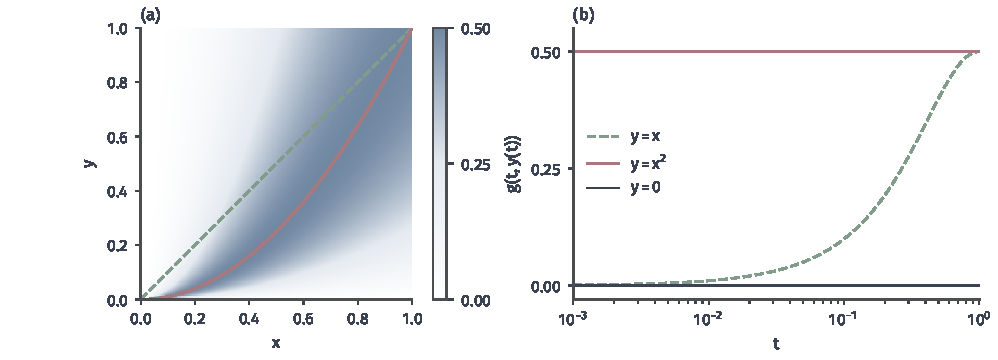
\includegraphics[width=169.0mm]{figures/01-mathematical-preliminaries-upper/00-shared/matplotlib/chapter3-concept-processes/joint-limit-paths.pdf}
 \caption{取前例$g(x,y)=x^2y/(x^4+y^2)$，原点另置零。(a) 第一象限的函数值及三条路径，色阶固定为$0$至$1/2$。(b) 沿$y=0$、$y=x$分别趋零，沿$y=x^2$恒为$1/2$；横轴为正参数$t$的对数刻度，向左趋近原点。不同路径极限足以否定联合极限，有限条路径不能反向证明存在。}
 \label{fig:analysis-process-joint-limit-paths}
\end{figure*}

\paragraph{累次极限与联合极限}
另一种常见做法是逐个坐标取极限，即累次极限。它改变了问题的量词：先令$y\to0$、再令$x\to0$，考察的是
$\lim_{x\to0}\lim_{y\to0}f(x,y)$。内层固定$x\neq0$，让$y$单独趋于$0$；得到一个关于$x$的函数后，外层再让$x$趋于$0$。整个过程没有要求两个坐标同时趋近。
对示例~\ref{ex:multivariable-path-limits}中的$f$，固定$x\neq0$时$f(x,y)\to0$，再令$x\to0$仍为$0$；交换次序同样得到$0$。两个次序的累次极限都为$0$，联合极限却不存在。

累次极限的次序本身也会影响结果。
\begin{example}[两个次序的累次极限不相等]
\label{ex:multivariable-iterated-limits-differ}
在非原点处令$h(x,y)=x^2/(x^2+y^2)$。固定$x\neq0$而令$y\to0$，得到$x^2/x^2=1$；固定$y\neq0$而令$x\to0$，得到$0$。再取外层极限，
\[
 \lim_{x\to0}\lim_{y\to0}h(x,y)=1,
 \qquad
 \lim_{y\to0}\lim_{x\to0}h(x,y)=0.
\]
内层先把一个坐标压到零，相当于先走到某条坐标轴附近，再沿坐标轴靠近原点。$h$在$x$轴上恒为$1$、在$y$轴上恒为$0$，两种次序因而给出不同结果。
\end{example}

所以累次极限相等不是联合极限存在的充分条件，改变次序也可能改变累次极限。

反方向在补充条件下成立：若联合极限$\lim_{(x,y)\to(0,0)}f(x,y)=L$存在，并且对充分接近$0$的每个$x\neq0$，内层极限$\lim_{y\to0}f(x,y)$都存在，则累次极限$\lim_{x\to0}\lim_{y\to0}f(x,y)$也存在且等于$L$。理由是：给定$\varepsilon>0$，取联合极限定义中的$\delta$；当$0<|x|<\delta/2$、$0<|y|<\delta/2$时$|f(x,y)-L|<\varepsilon$，令$y\to0$，内层极限与$L$相差不超过$\varepsilon$。

\paragraph{统一误差估计}
要证明联合极限存在，可以寻找只依赖距离的上界：若$|f(\bm x)-L|$不超过一个只与$\lVert\bm x-\bm a\rVert_2$有关、并随距离趋于零的量，所有路径就同时受到控制。
\begin{example}[用距离上界证明联合极限]
\label{ex:multivariable-distance-bound-limit}
在非原点处考虑$x^2y/(x^2+y^2)$。由$|xy|\leq(x^2+y^2)/2$，有
\[
 \left|\frac{x^2y}{x^2+y^2}\right|
 =|x|\cdot\frac{|xy|}{x^2+y^2}
 \leq \frac{|x|}{2}
 \leq\frac12\sqrt{x^2+y^2}.
\]
给定$\varepsilon>0$，取$\delta=2\varepsilon$，则距离原点小于$\delta$的非原点都满足误差小于$\varepsilon$，因此原点处极限为$0$。

改用极坐标$(x,y)=(r\cos\theta,r\sin\theta)$，同一函数等于$r\cos^2\theta\sin\theta$，绝对值不超过$r$。这个界对所有$\theta$同时成立，给出同样的结论。
\end{example}

极坐标估计有效的关键是界与角度无关。若只固定$\theta$再令$r\to0$，检查的仍然只是直线。
\begin{example}[固定角度的极坐标检验]
\label{ex:multivariable-polar-fixed-angle}
对示例~\ref{ex:multivariable-parabola-path-limit}中的$g$，代入$(x,y)=(r\cos\theta,r\sin\theta)$得到
\[
 g=\frac{r\cos^2\theta\sin\theta}{r^2\cos^4\theta+\sin^2\theta}.
\]
固定$\theta$再令$r\to0$：$\sin\theta\neq0$时分母趋于$\sin^2\theta$而分子趋于$0$，$\sin\theta=0$时函数恒为$0$，结果总是$0$。
但对每个小的$r>0$，可以取满足$\sin\theta=r\cos^2\theta$的角度。此时分子等于$r^2\cos^4\theta$、分母等于$2r^2\cos^4\theta$，函数值恰为$1/2$。这个角度随$r$改变，对应的点$(r\cos\theta,r\sin\theta)$满足$y=r^2\cos^2\theta=x^2$，正好落在抛物线上。
\end{example}

因此用极坐标证明联合极限时，需要一个对全部$\theta$同时成立、并随$r\to0$趋于零的界。

\subsubsection{连续性的定义与运算}
\label{sec:multivariable-continuity}

连续性要求输入联合趋近基点时，输出趋于基点处的函数值。定义形式与一元连续性相同，只是把$|x-a|$换成欧氏距离；给出定义后，再检验和、差、数乘、积、商与复合是否保持连续性。
\begin{definition}[多元标量函数的连续性]
\label{def:multivariable-scalar-continuity}
设$f:D\subseteq\mathbb R^d\to\mathbb R$、$\bm a\in D$。若对每个$\varepsilon>0$都存在$\delta>0$，使
\[
 \bm x\in D,\quad\lVert\bm x-\bm a\rVert_2<\delta
 \Longrightarrow |f(\bm x)-f(\bm a)|<\varepsilon,
\]
则称$f$在$\bm a$处连续；在$D$上每点连续时称$f$为连续函数。
\end{definition}
在聚点处，这等价于联合极限等于$f(\bm a)$；在孤立点处，取足够小的$\delta$使球内只有$\bm a$，定义自动成立。
几何上，连续意味着曲面在$\bm a$上方没有裂缝或跳跃：从任何方向走近，高度都平稳地接近$f(\bm a)$。
固定其他输入坐标后的一元切片连续只是必要条件，示例~\ref{ex:multivariable-path-limits}说明它不足以保证联合连续。

\paragraph{和的连续性}
设$f,g$在$\bm a$处连续。由三角不等式，
\[
 |(f+g)(\bm x)-(f+g)(\bm a)|\leq|f(\bm x)-f(\bm a)|+|g(\bm x)-g(\bm a)|.
\]
给定$\varepsilon>0$，分别取使两个误差都小于$\varepsilon/2$的半径，其中较小的半径就满足$f+g$的连续性要求。

\paragraph{差的连续性}
相减时两项的误差仍按三角不等式相加：$|(f-g)(\bm x)-(f-g)(\bm a)|\leq|f(\bm x)-f(\bm a)|+|g(\bm x)-g(\bm a)|$。取与和相同的半径，即得$f-g$在$\bm a$处连续。

\paragraph{数乘的连续性}
对固定实数$c$，有$|cf(\bm x)-cf(\bm a)|=|c|\,|f(\bm x)-f(\bm a)|$。$c\neq0$时，把$f$的误差控制在$\varepsilon/|c|$以内即可；$c=0$时$cf$是常函数，结论直接成立。

\paragraph{积的连续性}
若$f,g$在$\bm a$处连续，乘积的误差可以拆成两项：
\[
 f(\bm x)g(\bm x)-f(\bm a)g(\bm a)
 =f(\bm x)\bigl(g(\bm x)-g(\bm a)\bigr)+g(\bm a)\bigl(f(\bm x)-f(\bm a)\bigr).
\]
由$f$的连续性，$\bm x$足够靠近$\bm a$时$|f(\bm x)|\leq|f(\bm a)|+1$，第一项的因子$f(\bm x)$有界；两个括号又都趋于零，所以$fg$在$\bm a$处连续。这与一元的乘积极限法则是同一个论证。

坐标函数$\bm x\mapsto x_j$连续，因为$|x_j-a_j|\leq\lVert\bm x-\bm a\rVert_2$。多元多项式由坐标函数和常数经有限次加法与乘法得到，因此连续，例如$x^2+xy+y^2$。

\paragraph{商的连续性}
除法还要防止分母变为零。若再设$g(\bm a)\neq0$，由$g$的连续性，可以取一个小球使其中$|g(\bm x)|>|g(\bm a)|/2$，即$g$在基点附近远离零。于是
\[
 \left|\frac1{g(\bm x)}-\frac1{g(\bm a)}\right|
 =\frac{|g(\bm x)-g(\bm a)|}{|g(\bm x)|\,|g(\bm a)|}
 \leq\frac{2|g(\bm x)-g(\bm a)|}{g(\bm a)^2}\longrightarrow0,
\]
所以$1/g$在$\bm a$处连续，再用积的连续性得到$f/g$连续。分母非零的条件不能省略，否则商在基点没有定义；由此，有理函数在分母非零处连续。

\paragraph{标量复合函数}
若$f:D\to\mathbb R$在$\bm a$处连续，一元函数$\psi$在$f(\bm a)$处连续，且$f$在$\bm a$附近的输出都在$\psi$的定义域内，则$\psi\circ f$在$\bm a$处连续。
证明分两步控制误差。给定$\varepsilon>0$，先由$\psi$的连续性取$\eta>0$，使中间实数与$f(\bm a)$相差小于$\eta$时，$\psi$的输出误差小于$\varepsilon$；再由$f$的连续性取$\delta>0$，使输入距离小于$\delta$时，$f$的输出与$f(\bm a)$相差小于$\eta$。合并两步，$\lVert\bm x-\bm a\rVert_2<\delta$时就有$|\psi(f(\bm x))-\psi(f(\bm a))|<\varepsilon$。
例如$e^{-(x^2+y^2)}$和$\sqrt{1+x^2+y^2}$都是一元连续函数与多项式的复合，因而在整个平面上连续。

\subsubsection{闭有界集上连续函数的性质}

寻找多元函数的最小值之前，先要知道最小值在什么条件下一定存在。机器学习中常在一块参数区域内最小化损失，如果最小值根本取不到，“求最小点”就没有对象。
一元情形中，闭区间上的连续函数一定取到最值，所用的关键事实是：闭区间内任意点列都有收敛于该区间内的子列。本小节先把这一子列性质推广到$\mathbb R^d$的闭有界集，再用它得到多元极值定理。

\paragraph{有限维闭有界集的收敛子列}
实数列的Bolzano--Weierstrass定理可以逐个坐标使用，得到多维输入所需的子列性质：有界性保证收敛子列存在，闭性保证极限点仍在集合内。
\begin{theorem}[有限维有界序列的收敛子列]
\label{thm:multivariable-bolzano-weierstrass}
若$(\bm x_n)$是$\mathbb R^d$中的有界序列，则存在严格递增的正整数序列$(n_k)$及$\bm a\in\mathbb R^d$，使$\bm x_{n_k}\to\bm a$。
若所有$\bm x_n$属于闭集$K$，则$\bm a\in K$。
\end{theorem}
\begin{proof}
序列有界，所以每个坐标组成的实数列也有界。以$d=2$为例：先用实数列定理，从第一坐标中选出收敛子列；在这个子列中，第二坐标仍是有界实数列，再从中选出收敛的子子列。子子列的第一坐标是收敛数列的子列，仍然收敛，因此两个坐标都收敛。一般的$d$重复这一步$d$次，每次都在上一步的子列中继续选取，最后全部坐标都收敛。
设各坐标极限组成$\bm a$，由$\lVert\bm x-\bm a\rVert_2\leq\sqrt d\max_j|x_j-a_j|$可知所得子列在欧氏距离下收敛于$\bm a$。
若所有项都属于闭集$K$，闭集包含其收敛序列的极限，故$\bm a\in K$。
\end{proof}
有限维闭有界集因此具有与闭区间相同的子列性质，极值定理的证明直接使用这一性质；一般度量空间中紧致与序列紧致的等价在第~\ref{chap:metric-spaces}章讨论。

\paragraph{有界性与极值达到}
要保证上、下确界由定义域内的点取得，需要防止“函数值趋近确界的输入序列”逃出定义域：它可能跑向无穷远，也可能趋向一个不属于定义域的边界点。
闭有界集的子列性质同时排除了这两种情况。
\begin{theorem}[闭有界集上的极值定理]
\label{thm:multivariable-extreme-value}
设$K\subseteq\mathbb R^d$非空、闭且有界，$f:K\to\mathbb R$连续，则$f$有界，且存在$\bm x_{\min},\bm x_{\max}\in K$满足
\[
 f(\bm x_{\min})\leq f(\bm x)\leq f(\bm x_{\max})\qquad(\bm x\in K).
\]
\end{theorem}
\begin{proof}
定理~\ref{thm:analysis-extreme-value}的证明只用到两件事：定义域内任意点列有收敛于定义域内的子列，以及函数连续。
这里的$K$由定理~\ref{thm:multivariable-bolzano-weierstrass}满足同一子列条件，输出仍为实数，所以该证明逐字适用。例如对最大值，取$\bm x_n\in K$使$f(\bm x_n)$趋于上确界，选出收敛子列$\bm x_{n_k}\to\bm x_{\max}\in K$，连续性给出$f(\bm x_{\max})$等于上确界。
\end{proof}
定理的条件只是充分条件，但删去其中任何一个，结论都可能失败。与一元的示例~\ref{ex:analysis-extrema-failures}相同，可以逐项构造反例。
\begin{example}[删去闭性、有界性或连续性时最值可能取不到]
\label{ex:multivariable-extreme-value-failures}
在开单位圆盘$\{x^2+y^2<1\}$上，连续函数$f(x,y)=x^2+y^2$的上确界为$1$，但趋近上确界的点跑向不属于圆盘的边界圆，最大值取不到；这说明不能删去闭性。
在闭而无界的整个平面上，$f(x,y)=-(x^2+y^2)$在远处无限变小，没有下界；这说明不能删去有界性。
在闭单位圆盘上，令$f(x,y)=x^2+y^2$（$x^2+y^2<1$），并在边界圆上令$f=0$。定义域闭且有界，但$f$在边界圆上不连续，上确界$1$仍取不到；这说明不能删去连续性。
\end{example}

一元情形中讨论过的一致连续，换用欧氏距离后可以同样定义，闭有界集上的连续函数一致连续的结论也照样成立，本节不再展开。Lipschitz条件则在可微性之后结合中值定理讨论。

\subsection{偏导数和梯度}

本小节仍研究实值函数$f:U\subseteq\mathbb R^d\to\mathbb R$，并要求$U$为开集。开集中每一点都有一个含于$U$的小球，从基点出发向任何方向走足够小的一步仍在定义域内，双侧差商因而都有意义。
本小节先计算各坐标切片的变化率，再把这些数排列为梯度，最后定义沿一般方向的变化率。

\subsubsection{偏导数}

固定除$x_j$以外的全部坐标，$f$就变成只依赖$x_j$的一元函数，可以直接使用一元导数。
\begin{definition}[偏导数]
\label{def:multivariable-partial-derivative}
设$\bm a\in U$，令$\bm e_j$是第$j$个坐标为$1$、其余为$0$的向量。若双侧极限
\[
 \partial_jf(\bm a)=\frac{\partial f}{\partial x_j}(\bm a)
 =\lim_{t\to0}\frac{f(\bm a+t\bm e_j)-f(\bm a)}t
\]
存在且有限，就称它为$f$在$\bm a$处关于$x_j$的\term{偏导数}（partial derivative）。
\end{definition}
偏导数表示只改变第$j$个坐标、其余坐标固定时的变化率。符号$\partial$提醒我们：这里求的是多元函数的一个坐标切片的导数。
几何上，对二元函数，$\partial_xf(a,b)$是用竖直平面$y=b$截曲面所得曲线在$x=a$处的切线斜率；$\partial_yf(a,b)$则来自平面$x=a$的截线。把$f$看成平板上的温度，$\partial_xf$就是向正东方向移动时温度每单位距离的变化。

计算偏导数时，把其余坐标当作常数，按一元函数求导即可。
\begin{example}[二次函数的偏导数]
\label{ex:multivariable-quadratic-partials}
对$f(x,y)=x^2+xy+y^2$，把$y$当作常数对$x$求导，得到$f_x=2x+y$；把$x$当作常数对$y$求导，得到$f_y=x+2y$。
在$(1,2)$处，两者分别为$4$和$5$。直接用定义核对第一个值：
\[
 \frac{f(1+t,2)-f(1,2)}t=\frac{(1+t)^2+2(1+t)+4-7}{t}=4+t\longrightarrow4.
\]
再用数值核对：$f(1.01,2)=7.0401$，比$f(1,2)=7$大约$0.04=4\times0.01$；$f(1,2.01)=7.0501$，大约增加$5\times0.01$。
\end{example}

$f_x(1,2)=4$并不意味着朝任何方向走都以斜率$4$变化，每个偏导数只描述自己那条坐标切片。若同时走$(0.01,0.01)$，则$f(1.01,2.01)=7.0903$，增量约为$0.04+0.05$，像是两个偏导数贡献之和。这种“可以相加”并非总是成立，后面的可微性正是为它提供保证。

\subsubsection{梯度}

各偏导数在同一基点计算，但分别对应不同输入坐标。将这些变化率按坐标顺序排成一列，就能用一个向量记录所有坐标切片的信息。
\begin{definition}[梯度]
\label{def:multivariable-gradient}
若$f:U\to\mathbb R$在$\bm a$处的各一阶偏导数都存在，称列向量
\[
 \nabla f(\bm a)=\bigl(\partial_1f(\bm a),\ldots,\partial_df(\bm a)\bigr)^\top
\]
为$f$在$\bm a$处的\term{梯度}（gradient）。
\end{definition}
由示例~\ref{ex:multivariable-quadratic-partials}，$f(x,y)=x^2+xy+y^2$的梯度为$\nabla f(x,y)=(2x+y,x+2y)^\top$，所以$\nabla f(1,2)=(4,5)^\top$。
梯度与输入属于同一个空间：$(4,5)^\top$可以画成地图平面上从$(1,2)$出发的一支箭头，而不是曲面上的向量。
就定义而言，梯度只是把各坐标的变化率并排放在一起。它能否预测所有坐标同时改变时的函数增量，箭头的方向又有什么含义，要等到第~\ref{sec:multivariable-total-differentiation}节的可微性才能回答。

\subsubsection{方向导数}

沿坐标轴求导只考察了$d$个方向。若让多个坐标按一个固定向量的比例共同移动，就得到另一条直线上的一元切片。
\begin{definition}[方向导数]
\label{def:multivariable-directional-derivative}
给定向量$\bm v\in\mathbb R^d$，若双侧极限
\[
 D_{\bm v}f(\bm a)
 =\lim_{t\to0}\frac{f(\bm a+t\bm v)-f(\bm a)}t
\]
存在且有限，就称它为沿$\bm v$的\term{方向导数}（directional derivative）。
\end{definition}
回到地形的比喻：站在$\bm a$上方，沿地图上的方向$\bm v$前进，方向导数就是脚下的坡度。
本书允许$\bm v$不是单位向量，这时导数按参数$t$的变化计量：$t$增加$1$，水平位置移动$\lVert\bm v\rVert_2$。若要表示每单位水平距离的变化率，应取$\lVert\bm v\rVert_2=1$。
取$\bm v=\bm e_j$便回到偏导数。双侧极限与只令$t\downarrow0$的单侧方向导数要分别判断。

方向向量的长度会改变方向导数的数值，比较同一条直线的两种参数化就能看清这一点。
\begin{example}[沿对角方向的方向导数]
\label{ex:multivariable-diagonal-directional-derivative}
仍取$f(x,y)=x^2+xy+y^2$，从$(1,2)$沿$\bm v=(1,1)^\top$移动，展开得
\[
 f(1+t,2+t)=(1+t)^2+(1+t)(2+t)+(2+t)^2=7+9t+3t^2,
\]
所以$D_{\bm v}f(1,2)=9$。
改用同向单位向量$\bm u=(1,1)^\top/\sqrt2$，参数$t$增加$1$时只走过单位距离，变化率为$D_{\bm u}f(1,2)=9/\sqrt2\approx6.36$。
\end{example}

两个方向向量描述同一条直线，但参数速度不同，比较变化率时不能忽略归一化约定。
还可以注意到$9=4\cdot1+5\cdot1$，恰是梯度$(4,5)^\top$与$\bm v$的内积。这不是巧合，但也并非所有函数都满足；下一小节说明它成立的条件。

\subsection{多元标量函数的可微性}
\label{sec:multivariable-total-differentiation}

偏导数和方向导数分别检查固定的坐标轴或直线。若要同时控制任意小扰动，包括方向不断改变的扰动，就需要一个对所有扰动共同有效的线性近似。

\subsubsection{微分的定义}

一元可微的含义是$f(a+h)=f(a)+f'(a)h+o(h)$：在$a$附近，函数图像可以用一条切线代替，误差比$h$小得多。把图像放大来看，曲线越来越像一条直线。
两个输入时，与切线对应的是切平面。把曲面$z=f(x,y)$在一点附近不断放大，如果它越来越像一张平面，就说$f$在该点可微，这张平面给出函数增量的最佳线性近似。

预测增量的规则应与扰动的叠加和数乘相容，因此使用线性映射$A:\mathbb R^d\to\mathbb R$。
例如$A(\bm h)=\bm c^\top\bm h$把每个坐标的扰动乘以固定系数再相加。可微性还要求遗漏的误差比扰动长度小得多。
\begin{definition}[多元标量函数的可微性与全微分]
\label{def:multivariable-total-differential}
设$U\subseteq\mathbb R^d$开，$f:U\to\mathbb R$，$\bm a\in U$。
若存在一个线性映射$A:\mathbb R^d\to\mathbb R$，使
\begin{equation}
 f(\bm a+\bm h)=f(\bm a)+A(\bm h)+o(\lVert\bm h\rVert_2),
 \qquad\bm h\to\bm0,
\label{eq:analysis-total-differentiability}
\end{equation}
则称$f$在$\bm a$处\term{可微}（differentiable）。线性映射$A$称为该点的\term{全微分}（total differential），记为$\mathrm df_{\bm a}$。
\end{definition}
余项条件是$|f(\bm a+\bm h)-f(\bm a)-A(\bm h)|/\lVert\bm h\rVert_2\to0$，其中$\bm h\to\bm 0$按第~\ref{sec:multivariable-joint-limits}节的联合极限理解。
它要求同一个$A$适用于全部趋零扰动，而不是先固定一个方向、再让误差控制随方向改变。
$d=2$时，$z=f(\bm a)+A(\bm x-\bm a)$是三维空间中经过$(\bm a,f(\bm a))$的一张平面，即切平面；余项条件说的是，曲面与切平面的高度差比到$\bm a$的水平距离小得多。

这个“小得多”可以用数值观察。
\begin{example}[切平面误差随步长缩小]
\label{ex:multivariable-tangent-plane-error}
对$f(x,y)=x^2+xy+y^2$在$(1,2)$处，取线性映射$A(h,k)=4h+5k$（示例~\ref{ex:multivariable-quadratic-differential}将证明它就是全微分）。
取$(h,k)=(0.01,0.02)$，切平面预测$7+0.04+0.10=7.14$，实际值$f(1.01,2.02)=7.1407$，误差为$0.0007$，与步长$\sqrt{0.01^2+0.02^2}\approx0.0224$之比约为$0.031$。
把步长减半为$(0.005,0.01)$，误差变为$0.000175$，与步长$\approx0.0112$之比约为$0.016$，也减半。
\end{example}

误差与步长之比随步长减半而减半；步长继续缩小时，这个比值趋于零，这正是余项条件的要求。

\subsubsection{可微性的要求与判别}
\label{sec:analysis-differentiability-relations}

本小节固定开集$U\subseteq\mathbb R^d$、标量函数$f:U\to\mathbb R$与基点$\bm a\in U$。
先说明统一线性近似必然满足哪些要求，并由此得到梯度的几何意义；再给出可核查的充分判别；最后用蕴含关系与反例区分偏导数存在、全部双侧方向导数存在、可微和连续可微。

\paragraph{可微的必要条件}
若同一个线性近似对全部扰动有效，把扰动限制在一条直线上，它就必须与这条直线上的一元导数相同；函数增量本身也必须趋于零。
这两点把全微分与偏导数、梯度及方向导数联系起来。
\begin{theorem}[可微性与梯度、方向导数]
\label{thm:multivariable-differentiable-necessary}
若$f:U\to\mathbb R$在$\bm a$处可微，则$f$在该点连续，各偏导数存在，并且
\[
 \mathrm df_{\bm a}(\bm h)=\nabla f(\bm a)^\top\bm h,
 \qquad D_{\bm v}f(\bm a)=\nabla f(\bm a)^\top\bm v
 \quad(\bm v\in\mathbb R^d).
\]
\end{theorem}
\begin{proof}
记$A=\mathrm df_{\bm a}$。先证连续。把$\bm h$按标准基写成$\sum_jh_j\bm e_j$，线性性给出$A(\bm h)=\sum_jh_jA(\bm e_j)$。由有限和的Cauchy--Schwarz不等式，
\[
 |A(\bm h)|\leq\left(\sum_j|A(\bm e_j)|^2\right)^{1/2}\lVert\bm h\rVert_2.
\]
因此在式~\eqref{eq:analysis-total-differentiability}中，线性项与余项都随$\bm h\to\bm 0$而趋零，即$f(\bm a+\bm h)\to f(\bm a)$，$f$连续。

再求系数。取$\bm h=t\bm e_j$，式~\eqref{eq:analysis-total-differentiability}变成$f(\bm a+t\bm e_j)-f(\bm a)=tA(\bm e_j)+o(|t|)$；两边除以$t$并令$t\to0$，可知偏导数存在且$\partial_jf(\bm a)=A(\bm e_j)$。代回线性展开，得到$A(\bm h)=\sum_j\partial_jf(\bm a)h_j=\nabla f(\bm a)^\top\bm h$。
最后对固定的$\bm v\neq\bm0$取$\bm h=t\bm v$：差商等于$\nabla f(\bm a)^\top\bm v$加上余项除以$t$，而余项是$o(|t|\lVert\bm v\rVert_2)$，除以$t$后仍趋零，就得到方向导数公式；$\bm v=\bm0$时差商恒为零。
\end{proof}
这个定理说明，一旦可微，全微分没有别的选择，只能是“梯度与扰动的内积”；所有方向导数也都由$d$个偏导数线性地决定。
因此验证可微时，候选线性映射已由梯度确定，只需再估计余项。对本节的二次函数，这一步可以直接完成。
\begin{example}[二元二次函数的全微分]
\label{ex:multivariable-quadratic-differential}
对二次函数$f(x,y)=x^2+xy+y^2$，在$(1,2)$处有$\nabla f=(4,5)^\top$。设扰动为$(h,k)$，直接展开得
\[
 f(1+h,2+k)=7+4h+5k+(h^2+hk+k^2).
\]
由$|hk|\leq(h^2+k^2)/2$，最后一项绝对值不超过$3(h^2+k^2)/2$；除以$\sqrt{h^2+k^2}$后不超过$\tfrac32\sqrt{h^2+k^2}$，随扰动趋于零。所以全微分确为$\mathrm df_{(1,2)}(h,k)=4h+5k$，切平面为$z=7+4(x-1)+5(y-2)$。
\end{example}

这个全微分同时给出了示例~\ref{ex:multivariable-quadratic-partials}中的两个偏导数，以及示例~\ref{ex:multivariable-diagonal-directional-derivative}中沿$(1,1)^\top$的变化率$4+5=9$。
图~\ref{fig:analysis-process-total-differential-remainder}将这个全微分的切平面与统一余项界对应起来。
\begin{figure*}[!htbp]
 \centering
 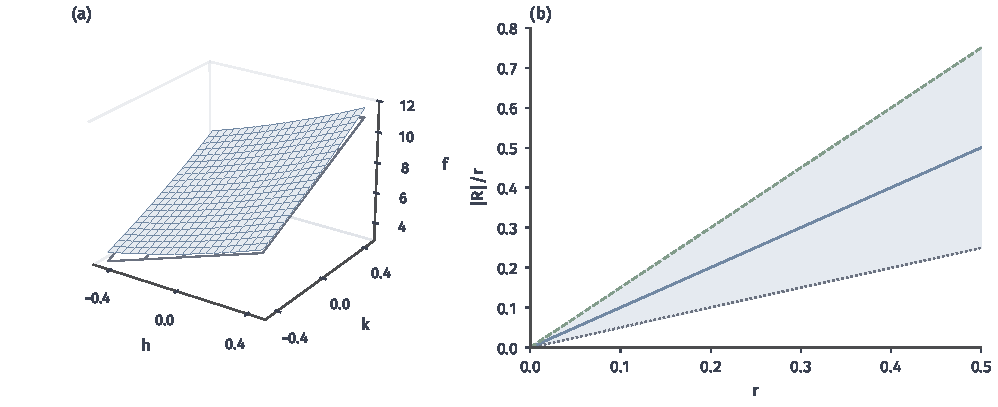
\includegraphics[width=169.0mm]{figures/01-mathematical-preliminaries-upper/00-shared/matplotlib/chapter3-concept-processes/total-differential-remainder.pdf}
 \caption{(a) 二次函数在$(1,2)$附近，灰网格是切平面$P=7+4h+5k$，蓝面是$f(1+h,2+k)$。(b) 令$r=\sqrt{h^2+k^2}$，余项$R=h^2+hk+k^2$满足$r/2\leq R/r\leq3r/2$；阴影给出所有方向的完整范围，三条线是其中的代表值。共同上界随$r\to0$趋零，才保证任意方向都适用同一个线性近似。}
 \label{fig:analysis-process-total-differential-remainder}
\end{figure*}

方向导数公式还说明了梯度指向哪里。设$f$在$\bm a$处可微，对单位方向$\bm u$，由内积不等式，$D_{\bm u}f(\bm a)=\nabla f(\bm a)^\top\bm u\leq\lVert\nabla f(\bm a)\rVert_2$。
梯度非零时，取$\bm u=\nabla f(\bm a)/\lVert\nabla f(\bm a)\rVert_2$即达到等号，所以梯度方向是局部上升最快的单位方向。
这些结论都需要可微性，不能只由梯度向量存在推出。

图~\ref{fig:analysis-process-gradient-level-curves}用同一个二次函数比较梯度方向、等值曲线切向及另一个单位方向。
\begin{figure}[!htbp]
 \centering
 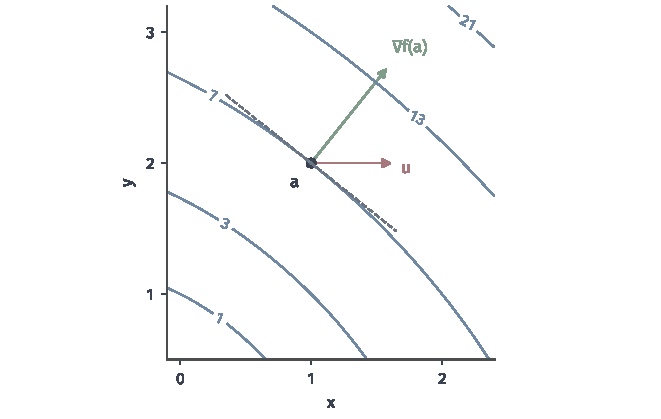
\includegraphics[width=112.0mm]{figures/01-mathematical-preliminaries-upper/00-shared/matplotlib/chapter3-concept-processes/gradient-level-curves.pdf}
 \caption{$f=x^2+xy+y^2$的等值曲线，标注为函数值；基点$a=(1,2)$处$\nabla f=(4,5)^\top$，图中绿箭头按$0.15$倍绘制。灰虚线沿$(5,-4)^\top$，与梯度垂直，因而与经过$a$的等值曲线相切；红箭头为$u=(1,0)^\top$。比较最快上升方向时须先归一化，不能直接比较图中箭头长度。}
 \label{fig:analysis-process-gradient-level-curves}
\end{figure}

\paragraph{偏导数连续给出的充分条件}
按定义验证可微，需要估计余项，通常不方便。另一种判别只检查偏导数：如果各坐标的变化率在基点附近连续变化，就可以沿坐标逐段走，用它们共同控制全部坐标增量。
与定理~\ref{thm:multivariable-differentiable-necessary}的必要条件不同，这项条件直接保证全微分存在。
\begin{theorem}[偏导数连续与可微性]
\label{thm:multivariable-continuous-partials-sufficient}
设$f:U\to\mathbb R$，$U$开，$\bm a\in U$。若各一阶偏导数在$\bm a$的某个邻域内存在，并在$\bm a$处连续，则$f$在$\bm a$处可微。
\end{theorem}
\begin{proof}
先看$d=2$。从$(a_1,a_2)$走到$(a_1+h_1,a_2+h_2)$，可以先竖直走、再水平走：
\[
 \begin{aligned}
 f(a_1+h_1,a_2+h_2)-f(a_1,a_2)
 &=\bigl[f(a_1+h_1,a_2+h_2)-f(a_1,a_2+h_2)\bigr]\\
 &\quad+\bigl[f(a_1,a_2+h_2)-f(a_1,a_2)\bigr].
 \end{aligned}
\]
第一个方括号只改变第一个坐标，对一元函数$s\mapsto f(s,a_2+h_2)$用中值定理，得到它等于$\partial_1f(\bm\xi_1)h_1$，其中$\bm\xi_1$在这段水平线段上；第二个方括号同理等于$\partial_2f(\bm\xi_2)h_2$，$\bm\xi_2$在竖直线段上。这里用到$\bm h$足够小时两段都在偏导数存在的邻域内。

一般的$d$同样把$\bm a$到$\bm a+\bm h$的增量拆成$d$段，每段只改一个坐标，一元中值定理将第$j$段增量写成$\partial_jf(\bm\xi_j)h_j$，$\bm\xi_j$是第$j$段上的中间点。
减去候选线性项后，误差为$\sum_j\bigl(\partial_jf(\bm\xi_j)-\partial_jf(\bm a)\bigr)h_j$，因此
\[
 \begin{aligned}
 &\left|f(\bm a+\bm h)-f(\bm a)-\sum_{j=1}^d\partial_j f(\bm a)h_j\right|\\
 &\qquad\leq \max_j\left|\partial_j f(\bm\xi_j)-\partial_j f(\bm a)\right|
       \sum_{j=1}^d|h_j|
 =o(\lVert\bm h\rVert_2).
 \end{aligned}
\]
最后一步有两个依据：当$\bm h\to\bm0$时，所有中间点到$\bm a$的距离都不超过$\lVert\bm h\rVert_2$，偏导数在$\bm a$处连续，使最大值一项趋于零；另一方面$\sum_j|h_j|\leq\sqrt d\lVert\bm h\rVert_2$。
这样，各坐标方向上的变化就拼成了同一个有效的全微分。
\end{proof}
偏导数连续只是充分条件：可微仅要求函数增量具有统一的一阶近似，不要求这些系数随基点连续变化。实际计算中，若各偏导数在所论开集上由连续的表达式给出，例如多项式、分母非零的有理函数，以及它们与指数、正弦等连续函数的复合，就可以直接断定可微。

\paragraph{连续可微函数}
若还希望各点的一阶系数，即梯度，随基点连续变化，就需在一个范围内同时控制偏导数。
实值函数的各一阶偏导数在开集$U$上存在且连续时，称它在$U$上连续可微，记为$C^1(U)$；$C^k(U)$表示直至$k$阶的各偏导数都存在且连续。
定理~\ref{thm:multivariable-continuous-partials-sufficient}保证$C^1$函数处处可微，逆向并不成立，一元函数已经足以说明这一点。
\begin{example}[处处可微而导数无界]
\label{ex:multivariable-differentiable-not-c1}
在实轴上令$r(0)=0$，$x\neq0$时令$r(x)=x^2\sin(1/x^2)$。
由于$|r(h)/h|=|h\sin(1/h^2)|\leq|h|\to0$，有$r'(0)=0$；非零点按运算法则求导，得到
\[
 r'(x)=2x\sin(1/x^2)-\frac{2}{x}\cos(1/x^2).
\]
取$x_n=(2\pi n)^{-1/2}$，则$1/x_n^2=2\pi n$，$\sin$项为$0$、$\cos$项为$1$，于是$r'(x_n)=-2/x_n\to-\infty$。所以$r$处处可微，$r'$却在$0$附近无界，在$0$处不连续。
直观上，$r$的振幅被$x^2$压到零，图像在原点与横轴相切；但振荡越来越快，切线斜率剧烈摆动。
在多元情形令$f(\bm x)=r(x_1)$，就得到处处可微而非连续可微的标量函数。
\end{example}

这个例子还说明可微不保证局部Lipschitz连续：若$r$在原点的某个邻域内以$L$为Lipschitz常数，该邻域内每个差商的绝对值都不超过$L$，各点导数也就满足$|r'|\leq L$，与$r'(x_n)\to-\infty$矛盾。

\paragraph{条件之间的蕴含关系}
由必要条件与充分判别，可以把这些要求放在一起比较：
\[
 \begin{gathered}
 f\text{在}\bm a\text{的某邻域内连续可微}
 \ \Longrightarrow\ f\text{在}\bm a\text{处可微},\\
 f\text{在}\bm a\text{处可微}
 \ \Longrightarrow\ \text{全部双侧方向导数存在}
 \ \Longrightarrow\ \text{全部偏导数存在}.
 \end{gathered}
\]
第一条由定理~\ref{thm:multivariable-continuous-partials-sufficient}得到，第二条由定理~\ref{thm:multivariable-differentiable-necessary}得到，最后一条只须在全部方向中取坐标方向$\bm e_j$。
同一定理还说明，可微蕴含连续，并使方向导数关于方向成为同一个线性映射$\bm v\mapsto\nabla f(\bm a)^\top\bm v$。
第一行的前提涉及$\bm a$的整个邻域，其余条件只涉及基点$\bm a$本身；示例~\ref{ex:multivariable-differentiable-not-c1}已经说明，即使处处可微，也不能反推连续可微。

一元函数在一点的导数存在就等价于可微，因为实轴上只有一条直线可走。多元函数还须协调无穷多个输入方向以及弯曲的趋近路径，所以第二行的两个逆命题也不成立，以下依次给出反例。

\paragraph{偏导数存在不保证可微}
先看坐标偏导数：它们只约束两条坐标切片，并未控制其余方向或路径。
\begin{example}[偏导数存在但不可微]
\label{ex:analysis-partials-not-differentiable}
定义$f:\mathbb{R}^2\to\mathbb{R}$为
\[
 f(x,y)=
 \begin{cases}
  \dfrac{xy}{\sqrt{x^2+y^2}}, & (x,y)\neq(0,0),\\[6pt]
  0, & (x,y)=(0,0).
 \end{cases}
\]
沿两条坐标轴，函数恒为$0$，所以$\partial f/\partial x(0,0)=\partial f/\partial y(0,0)=0$。若$f$在原点可微，由定理~\ref{thm:multivariable-differentiable-necessary}，候选线性部分只能是零映射。可是沿$\bm{h}=(t,t)$，
\[
 \frac{|f(t,t)-f(0,0)|}{\lVert(t,t)\rVert_2}
 =\frac{|t|/\sqrt{2}}{\sqrt{2}|t|}
 =\frac12,
\]
余项与$\lVert\bm{h}\rVert_2$之比不趋于零，故$f$在原点不可微。

用极坐标可以看清曲面的形状：$f=r\cos\theta\sin\theta=\tfrac r2\sin2\theta$。沿每条从原点出发的射线，函数随$r$线性增长，斜率$\tfrac12\sin2\theta$随方向变化。曲面由这些射线组成，像一个起伏的锥面；把它放大任意倍数后形状不变，永远不会变得像一张平面。

沿每个方向$\bm v=(a,b)$，只令$t\downarrow0$的正向方向导数都存在，等于$ab/\sqrt{a^2+b^2}$（零方向取$0$），但它不是关于$\bm v$的线性函数。$t<0$时差商变号，因此$ab\neq0$时双侧方向导数不存在。
最后，由$|xy|/\sqrt{x^2+y^2}\leq\sqrt{x^2+y^2}/2$，$f$在原点连续。
\end{example}

偏导数只看坐标轴，遗漏了其他接近方向；可微则要求曲面放大后接近平面，本例的锥面做不到。这个例子还说明，偏导数存在、全部正向方向导数存在，再加上连续性，都不足以推出可微。方向极限采用单侧还是双侧，必须与所用定义一致；本节定义采用双侧极限。

\paragraph{全部方向导数存在不保证可微}
从坐标切片扩展到所有固定直线，仍需检查两件事：这些变化率能否组成一个线性映射，以及是否具有统一余项。先看缺少线性性的情形。
\begin{example}[方向导数不构成线性映射]
\label{ex:multivariable-nonlinear-directional-derivatives}
在非原点处令$p(x,y)=x^3/(x^2+y^2)$，并令$p(0,0)=0$。
沿$\bm v=(a,b)\neq\bm0$，差商为$p(ta,tb)/t=a^3/(a^2+b^2)$，不依赖$t$，所以双侧方向导数存在且$D_{\bm v}p(0,0)=a^3/(a^2+b^2)$。
取坐标方向得到候选梯度$(1,0)^\top$。若$p$可微，沿$(1,1)^\top$的方向导数应为$(1,0)(1,1)^\top=1$，实际却是$1/(1+1)=1/2$。这些方向变化率无法拼成一个线性映射，所以$p$在原点不可微。
\end{example}

与示例~\ref{ex:analysis-partials-not-differentiable}只有单侧方向极限不同，这里的双侧方向导数全部存在，失败只来自线性性。
即使方向导数全部存在并组成一个线性映射，仍需检查统一余项。
\begin{example}[所有方向导数为零仍不足以可微]
\label{ex:multivariable-linear-directionals-not-differentiable}
在非原点处令$q(x,y)=x^3y/(x^4+y^2)$，并令$q(0,0)=0$。
由$2|x^2y|\leq x^4+y^2$，有$|q(x,y)|\leq|x|/2$，故$q$在原点连续。
对固定方向$(a,b)^\top$，若$b\neq0$，
\[
 \frac{q(ta,tb)}t=\frac{t a^3b}{t^2a^4+b^2}\longrightarrow0;
\]
若$b=0$，差商恒为零。因此所有双侧方向导数都为零，它们组成零线性映射。
可是沿$\bm h=(t,t^2)^\top$，$q(t,t^2)=t^5/(2t^4)=t/2$，从而
\[
 \frac{|q(t,t^2)|}{\lVert(t,t^2)\rVert_2}
 =\frac1{2\sqrt{1+t^2}}\longrightarrow\frac12.
\]
候选零映射不满足全微分的余项条件，$q$在原点不可微。
\end{example}

这与示例~\ref{ex:multivariable-parabola-path-limit}中$g$的情形相同：函数沿抛物线有一道坡，每条直线进入原点时都避开了它。方向导数先固定方向再取极限，全微分则要求对方向随扰动改变的序列也有同一个误差控制。

\paragraph{连续不保证偏导数存在}
反过来，连续性也推不出微分条件。
例如$f(x,y)=|x|$在整个平面上Lipschitz连续，图像沿$y$轴有一道折痕，原点关于$x$的双侧偏导数不存在，因此在那里不可微。
偏导数存在同样推不出连续：示例~\ref{ex:multivariable-path-limits}中原点置零的$xy/(x^2+y^2)$沿坐标轴恒为零，两个偏导数存在，但它在原点不连续。
因此连续与偏导数存在之间互不蕴含；可微则同时保证二者。

\paragraph{梯度与线性近似的使用条件}
上述反例区分了梯度的两种用途。仅有偏导数时，梯度只是坐标变化率排成的向量；确认可微以后，才可用它统一预测增量，用内积计算任意方向导数，并把它解释为最快上升的方向。
连续偏导数提供方便的充分判别，却不是必要条件；不满足该判别时，应回到全微分的统一余项定义检查。
讨论向量值函数时，同样对各个标量输出分量分别检查，再组成Jacobian矩阵及复合微分。

\subsubsection{微分的运算法则}

本小节的$f,g$都在同一开集内定义，并在基点$\bm a$处可微，$c$为固定实数。
各法则的证明方法相同：把各自的一阶展开代入，整理出关于$\bm h$的线性项，再确认剩下的部分仍是$o(\lVert\bm h\rVert_2)$。这样既得到新函数可微，也读出了它的全微分。

\paragraph{和的微分}
把两个一阶展开相加，
\[
 (f+g)(\bm a+\bm h)=(f+g)(\bm a)+\bigl(\mathrm df_{\bm a}+\mathrm dg_{\bm a}\bigr)(\bm h)+o(\lVert\bm h\rVert_2),
\]
两个线性映射之和仍是线性映射，两个$o(\lVert\bm h\rVert_2)$余项之和仍是$o(\lVert\bm h\rVert_2)$，因此
\[
 \mathrm d(f+g)=\mathrm df+\mathrm dg,\qquad \nabla(f+g)=\nabla f+\nabla g.
\]

\paragraph{差的微分}
把加号换成减号，同样的论证给出
\[
 \mathrm d(f-g)=\mathrm df-\mathrm dg,\qquad \nabla(f-g)=\nabla f-\nabla g.
\]

\paragraph{数乘的微分}
固定系数$c$只会缩放线性项与余项，故
\[
 \mathrm d(cf)=c\,\mathrm df,\qquad \nabla(cf)=c\nabla f,
\]
包括$c=0$的常函数情形。

\paragraph{积的微分}
记$R_f,R_g$为两个一阶展开的余项，都是$o(\lVert\bm h\rVert_2)$。相乘得
\[
 \begin{aligned}
 f(\bm a+\bm h)g(\bm a+\bm h)
 &=\bigl(f(\bm a)+\mathrm df(\bm h)+R_f\bigr)\bigl(g(\bm a)+\mathrm dg(\bm h)+R_g\bigr)\\
 &=f(\bm a)g(\bm a)+g(\bm a)\,\mathrm df(\bm h)+f(\bm a)\,\mathrm dg(\bm h)+(\text{其余各项}).
 \end{aligned}
\]
其余各项要么含有余项$R_f,R_g$乘以有界量，要么是两个线性增量的乘积$\mathrm df(\bm h)\,\mathrm dg(\bm h)=O(\lVert\bm h\rVert_2^2)$，都是$o(\lVert\bm h\rVert_2)$。因此乘积可微，且
\[
 \mathrm d(fg)=g(\bm a)\,\mathrm df+f(\bm a)\,\mathrm dg.
\]
这与一元的$(fg)'=f'g+fg'$形式相同：两个因子各自变化，一阶上贡献可以相加，两个变化同时发生的部分是高阶小量。

\paragraph{商的微分}
设$g(\bm a)\neq0$。可微蕴含连续，所以$g$在$\bm a$附近远离零，$1/g$在$\bm a$附近有定义。记$\delta=g(\bm a+\bm h)-g(\bm a)=\mathrm dg(\bm h)+o(\lVert\bm h\rVert_2)$，它是$O(\lVert\bm h\rVert_2)$。一元函数$1/y$在$g(\bm a)$处的展开给出
\[
 \frac1{g(\bm a)+\delta}=\frac1{g(\bm a)}-\frac{\delta}{g(\bm a)^2}+O(\delta^2).
\]
代入$\delta$的展开，并注意$O(\delta^2)=O(\lVert\bm h\rVert_2^2)$，得到$\mathrm d(1/g)=-\mathrm dg/g(\bm a)^2$。再把$f/g$看成$f\cdot(1/g)$，用积的微分得到
\[
 \mathrm d(f/g)=\frac{g(\bm a)\,\mathrm df-f(\bm a)\,\mathrm dg}{g(\bm a)^2}.
\]
这里分母非零既是定义商函数的条件，也是估计余项的条件。

\paragraph{标量复合函数的微分}
若一元函数$\psi$在$f(\bm a)$处可微，且复合在$\bm a$的邻域内有定义，则$\psi\circ f$在$\bm a$处可微，并且
\[
 \mathrm d(\psi\circ f)=\psi'(f(\bm a))\,\mathrm df,
 \qquad
 \nabla(\psi\circ f)(\bm a)=\psi'(f(\bm a))\nabla f(\bm a).
\]
推导时把内层增量$\delta=f(\bm a+\bm h)-f(\bm a)$代入外层的一元展开$\psi(f(\bm a)+\delta)=\psi(f(\bm a))+\psi'(f(\bm a))\delta+o(|\delta|)$，再把$\delta=\mathrm df(\bm h)+o(\lVert\bm h\rVert_2)$代入。
因为$\delta=O(\lVert\bm h\rVert_2)$，外层余项$o(|\delta|)$仍是$o(\lVert\bm h\rVert_2)$。
例如$\nabla e^{-(x^2+y^2)}=e^{-(x^2+y^2)}(-2x,-2y)^\top$：外层只把内层梯度乘上一个正数，所以复合函数的梯度与$-(x^2+y^2)$的梯度同向，都指向原点。

\paragraph{二次型的微分}
向量自变量的二次型仍是标量函数，机器学习中的平方误差、能量函数等都含有这种结构。考虑$q(\bm{x})=\bm{x}^{\top}\bm{A}\bm{x}=\sum_{i,j}A_{i,j}x_ix_j$，其中$\bm{A}\in\mathbb{R}^{d\times d}$固定。它是有限个乘积的和，乘积法则可以直接使用：把两个$\bm x$看成两个因子，每次只让一个变化，
\begin{align*}
  \mathrm{d}q
  &=
  (\mathrm{d}\bm{x})^{\top}\bm{A}\bm{x}
  +\bm{x}^{\top}\bm{A}\,\mathrm{d}\bm{x}\\
  &=
  \bm{x}^{\top}(\bm{A}^{\top}+\bm{A})\,\mathrm{d}\bm{x}.
\end{align*}
第二步用到$(\mathrm d\bm x)^\top\bm A\bm x$是一个实数，等于自己的转置$\bm x^\top\bm A^\top\mathrm d\bm x$。把$\mathrm dq$写成$\nabla q^\top\mathrm d\bm x$的形式，就读出
\begin{equation}
  \nabla_{\bm{x}}
  \bigl(\bm{x}^{\top}\bm{A}\bm{x}\bigr)
  =
  (\bm{A}+\bm{A}^{\top})\bm{x}.
\label{eq:analysis-quadratic-form-gradient}
\end{equation}
当$\bm{A}$对称时，式~\eqref{eq:analysis-quadratic-form-gradient}化为$2\bm{A}\bm{x}$，与一元的$(ax^2)'=2ax$对应；$\bm A$不对称时直接写成$2\bm{A}\bm{x}$，等于悄悄加入了对称性条件。
例如$\bm A=\begin{bmatrix}0&1\\0&0\end{bmatrix}$时$q=x_1x_2$，直接求偏导得$\nabla q=(x_2,x_1)^\top$，与$(\bm A+\bm A^\top)\bm x$一致；而$2\bm A\bm x=(2x_2,0)^\top$是错的。

\subsubsection{中值定理}

导数控制一点处的变化；要估计两点之间的有限变化，可以沿连接两点的线段把函数限制为一元函数，再使用一元中值定理。前提是整条线段都在定义域内。
记$[\bm x,\bm y]=\{\bm x+t(\bm y-\bm x):0\leq t\leq1\}$为连接两点的线段。
\begin{theorem}[多元标量函数的中值公式]
\label{thm:multivariable-scalar-mean-value}
设$f$在包含$[\bm x,\bm y]$的开集上可微，$\bm x\neq\bm y$。则存在$\theta\in(0,1)$使
\[
 f(\bm y)-f(\bm x)=\nabla f(\bm x+\theta(\bm y-\bm x))^\top(\bm y-\bm x).
\]
\end{theorem}
\begin{proof}
令$\phi(t)=f(\bm x+t(\bm y-\bm x))$，$t\in[0,1]$，它是$f$在线段上的一元切片。$\phi'(t)$就是$f$在点$\bm x+t(\bm y-\bm x)$处沿$\bm y-\bm x$的方向导数，由定理~\ref{thm:multivariable-differentiable-necessary}，$\phi'(t)=\nabla f(\bm x+t(\bm y-\bm x))^\top(\bm y-\bm x)$。
对$\phi$在$[0,1]$上使用一元中值定理，$\phi(1)-\phi(0)=\phi'(\theta)$，这就是所述等式。
\end{proof}
等式说明，两点之间的平均变化率等于线段上某一点沿该方向的瞬时变化率，这是一元“平均斜率等于某点切线斜率”的直接推广。
例如$f(x,y)=x^2+y^2$，$\bm x=(0,0)$、$\bm y=(1,1)$，左侧为$2$；右侧为$\nabla f(\theta,\theta)^\top(1,1)^\top=4\theta$，取$\theta=1/2$即相等，中值点恰为线段中点。

\subsubsection{Lipschitz条件}

中值公式把有限增量写成某点梯度与位移的内积。若梯度的长度有统一上界，就能用输入距离的常数倍控制输出变化，这就是多元情形的Lipschitz条件。优化中常用它由步长控制函数值的变化。
\begin{definition}[多元函数的Lipschitz条件]
\label{def:multivariable-lipschitz}
设$D\subseteq\mathbb R^d$，$f:D\to\mathbb R$。若存在有限常数$L\geq0$，使
\[
 |f(\bm x)-f(\bm y)|\leq L\lVert\bm x-\bm y\rVert_2\qquad(\bm x,\bm y\in D),
\]
称$f$在$D$上Lipschitz连续，$L$称为Lipschitz常数。若每点都有一个邻域使$f$在其中Lipschitz连续（常数可随邻域改变），称$f$局部Lipschitz连续。
\end{definition}
这与一元定义只差把$|x-y|$换成欧氏距离。例如线性函数$f(\bm x)=\bm a^\top\bm x$满足$|f(\bm x)-f(\bm y)|=|\bm a^\top(\bm x-\bm y)|\leq\lVert\bm a\rVert_2\lVert\bm x-\bm y\rVert_2$，Lipschitz常数可取$\lVert\bm a\rVert_2$。欧氏范数$f(\bm x)=\lVert\bm x\rVert_2$由三角不等式满足$|\lVert\bm x\rVert_2-\lVert\bm y\rVert_2|\leq\lVert\bm x-\bm y\rVert_2$，常数为$1$，尽管它在原点不可微。

梯度界要转化为Lipschitz常数，还需要两点之间的线段留在定义域内。集合$D$称为凸集，是指其中任意两点之间的线段都含于$D$。在凸开集上，梯度长度的统一上界恰好就是Lipschitz常数。
\begin{theorem}[梯度有界与Lipschitz条件]
\label{thm:multivariable-gradient-lipschitz}
设$U\subseteq\mathbb R^d$为凸开集，$f:U\to\mathbb R$可微。则$f$在$U$上以$L$为Lipschitz常数，当且仅当$\lVert\nabla f(\bm x)\rVert_2\leq L$对所有$\bm x\in U$成立。
\end{theorem}
\begin{proof}
若梯度长度不超过$L$，任取$\bm x\neq\bm y$，凸性保证线段$[\bm x,\bm y]\subseteq U$。由中值公式与内积不等式，
\[
 |f(\bm y)-f(\bm x)|=\bigl|\nabla f(\bm\xi)^\top(\bm y-\bm x)\bigr|\leq\lVert\nabla f(\bm\xi)\rVert_2\lVert\bm y-\bm x\rVert_2\leq L\lVert\bm y-\bm x\rVert_2.
\]
反过来，设$f$以$L$为Lipschitz常数。固定$\bm x$，若$\nabla f(\bm x)\neq\bm0$，取单位方向$\bm u=\nabla f(\bm x)/\lVert\nabla f(\bm x)\rVert_2$，则
\[
 \lVert\nabla f(\bm x)\rVert_2=D_{\bm u}f(\bm x)=\lim_{t\downarrow0}\frac{f(\bm x+t\bm u)-f(\bm x)}t\leq\lim_{t\downarrow0}\frac{Lt}t=L.
\]
梯度为零时不等式自然成立。
\end{proof}
几何上，若坡度处处不超过$L$，沿直线走过距离$\rho$，高度最多改变$L\rho$；反过来，Lipschitz常数也限制了每一点最陡方向的坡度。
例如$f(x,y)=\sin x+\cos y$满足$\lVert\nabla f\rVert_2=\sqrt{\cos^2x+\sin^2y}\leq\sqrt2$，所以它在整个平面上以$\sqrt2$为Lipschitz常数。

定理中的凸性不能省略。在不凸的区域上，梯度可以处处很小，函数值却在两个很近的点之间相差很大。
\begin{example}[非凸区域上梯度有界而不Lipschitz]
\label{ex:multivariable-nonconvex-lipschitz-failure}
取去掉负$x$轴的环形区域$D=\{1<\lVert\bm x\rVert_2<2\}\setminus\{(x,0):x<0\}$，令$f(\bm x)$为点$\bm x$的极角，取值于$(-\pi,\pi)$。$f$在$D$上可微，$\lVert\nabla f\rVert_2=1/r<1$，坡度处处小于$1$。
但取负$x$轴两侧的点$(-1.5,\pm\varepsilon)$，两点距离为$2\varepsilon$，极角却分别接近$\pi$与$-\pi$，相差接近$2\pi$。令$\varepsilon\to0$，函数值之差与距离之比无界，所以$f$在$D$上不是Lipschitz函数。
\end{example}

连接这两点的直线段穿过被去掉的负$x$轴，不在$D$内，中值公式无法使用；$D$内连接两点的路径必须绕过原点，长度远大于$2\varepsilon$。梯度界只能沿含于定义域的线段转化为函数值之差的界。

局部情形同理。若$f\in C^1(U)$，在每个基点附近取一个包含在$U$内的闭球。连续函数$\lVert\nabla f\rVert_2$在这个闭有界集上有界（定理~\ref{thm:multivariable-extreme-value}），因而在同心的开球上也有界；开球是凸开集，故由定理~\ref{thm:multivariable-gradient-lipschitz}，$f$在这个开球上Lipschitz连续，从而局部Lipschitz连续。
局部常数不自动给出全域共同常数：$f(x,y)=x^2$连续可微，但$\lVert\nabla f\rVert_2=2|x|$在全平面无界，因而它不是全域Lipschitz函数。

\subsection{多元标量函数的高阶微分}
\label{sec:multivariable-curvature-error}

一阶微分用切平面描述局部变化，却看不出曲面向哪边弯：碗底、山顶和马鞍点处的切平面都是水平的。高阶微分记录一阶系数本身怎样变化，从而描述弯曲。
本小节先把二阶偏导数集中为Hessian矩阵，再用Taylor公式建立二阶近似，最后据此判断驻点的局部极值类型。

\subsubsection{二阶偏导数与Hessian矩阵}

一阶偏导数本身仍是多元标量函数，可以再次求偏导。这里记$f_{x_i x_j}=\partial_j(\partial_i f)$，即先对$x_i$、再对$x_j$求导。
$f_{xx}$描述$x$方向切片的斜率沿$x$方向怎样变化，即该切片的弯曲；混合偏导数$f_{xy}$描述$x$方向的斜率在沿$y$方向移动时怎样变化，即曲面的扭转。

对$f(x,y)=x^2+xy+y^2$，有$f_{xx}=2$、$f_{xy}=f_{yx}=1$、$f_{yy}=2$。又如$f(x,y)=xy$，$x$方向切片的斜率是$y$，向北每走一单位，这个斜率就增加$1$，故$f_{xy}=1$，而$f_{xx}=f_{yy}=0$：每条坐标切片都是直线，曲面却是扭曲的。
这两个例子中$f_{xy}=f_{yx}$，但一般函数的混合偏导数能否交换次序，需要额外条件。

\paragraph{混合偏导数的交换}
分别沿两个坐标求导时，先后次序未必无关。
\begin{example}[混合偏导数与求导次序有关]
\label{ex:multivariable-mixed-partials-differ}
令$f(0,0)=0$，非原点处令
\[
 f(x,y)=\frac{xy(x^2-y^2)}{x^2+y^2}.
\]
对$y\neq0$，因为$f(0,y)=0$，
\[
 f_x(0,y)=\lim_{h\to0}\frac{f(h,y)}h=\lim_{h\to0}\frac{y(h^2-y^2)}{h^2+y^2}=-y;
\]
又$f$在$x$轴上恒为$0$，故$f_x(0,0)=0$，公式$f_x(0,y)=-y$在$y=0$时也成立。同样算得$f_y(x,0)=x$对所有$x$成立。于是
\[
 f_{xy}(0,0)=\frac{\mathrm d}{\mathrm dy}(-y)\Big|_{y=0}=-1,
 \qquad
 f_{yx}(0,0)=\frac{\mathrm d}{\mathrm dx}x\Big|_{x=0}=1,
\]
两个次序给出不同结果。
\end{example}

定理~\ref{thm:multivariable-mixed-partials}将说明，混合偏导数在基点连续时两种次序一定相同；因此本例的混合偏导数不可能都在原点连续。
\begin{theorem}[混合偏导数的交换]
\label{thm:multivariable-mixed-partials}
设$f$在$\bm a$的某个开邻域内有一阶偏导数$\partial_i f,\partial_j f$，混合偏导数$\partial_j\partial_i f,\partial_i\partial_j f$在该邻域存在并在$\bm a$处连续，则
\[
 \partial_j\partial_i f(\bm a)=\partial_i\partial_j f(\bm a).
\]
特别地，$C^2$函数的混合偏导数处处可以交换。
\end{theorem}
\begin{proof}
固定其他坐标，只需讨论二元函数在$(a,b)$处的情形。对小的非零$h,k$考察小矩形四个顶点上的二阶差分
\[
 \Delta(h,k)=f(a+h,b+k)-f(a+h,b)-f(a,b+k)+f(a,b).
\]
它可以按两种方式分组：先比较上下两边的差，或先比较左右两边的差，两种分组各给出一个混合偏导数。

令$\phi(x)=f(x,b+k)-f(x,b)$，则$\Delta=\phi(a+h)-\phi(a)$。先对$\phi$用一元中值定理，得到$\Delta=h\phi'(\xi)=h[f_x(\xi,b+k)-f_x(\xi,b)]$；再对$y\mapsto f_x(\xi,y)$使用一次中值定理，得到
\[
 \Delta=h[f_x(\xi,b+k)-f_x(\xi,b)]=hk f_{xy}(\xi,\eta),
\]
其中$\xi$在$a,a+h$之间、$\eta$在$b,b+k$之间。改用$\psi(y)=f(a+h,y)-f(a,y)$先沿$y$方向拆分，同样得到$\Delta=hk f_{yx}(\xi',\eta')$。
于是$f_{xy}(\xi,\eta)=f_{yx}(\xi',\eta')$。令$h,k\to0$，两个中间点都趋于$(a,b)$，连续性使两种混合偏导数在该点相等。
\end{proof}
示例~\ref{ex:multivariable-mixed-partials-differ}说明，只有混合偏导数存在而没有这些连续性条件时，结论可能失败。

\paragraph{Hessian矩阵}
把全部二阶偏导数排成一个方阵，就得到记录二阶信息的矩阵，它的行、列分别对应先后两次求导的输入坐标。
\begin{definition}[Hessian矩阵]
\label{def:multivariable-hessian}
若$f:U\to\mathbb R$在$\bm x$附近有一阶偏导数，且各$\partial_j\partial_i f(\bm x)$存在，则称
\[
 \nabla^2f(\bm x)=\bigl[\partial_j\partial_i f(\bm x)\bigr]_{i,j=1}^d
\]
为$f$在该点的\term{Hessian矩阵}（Hessian matrix）。
\end{definition}
第$i$行是第$i$个偏导数$\partial_if$的梯度（转置后），所以Hessian也可以理解为“梯度的梯度”：它说明当基点移动时，梯度向量怎样变化。
二阶偏导数存在本身尚不保证梯度映射$\nabla f$具有统一的线性近似；二阶可微要求$\nabla f$本身可微。
$C^2$是保证二阶可微的充分条件，且由定理~\ref{thm:multivariable-mixed-partials}，此时Hessian对称。对$x^2+xy+y^2$，Hessian就是$\begin{bmatrix}2&1\\1&2\end{bmatrix}$。

一元函数的二阶导数描述曲线向上还是向下弯；多元函数可以沿每个方向分别看。若$f\in C^2$，沿直线$t\mapsto f(\bm x+t\bm v)$求两次导数，在$t=0$处得到
\[
 \bm v^\top\nabla^2f(\bm x)\bm v
 =\sum_{i=1}^d\sum_{j=1}^d \partial_j\partial_i f(\bm x)v_i v_j.
\]
这一计算的依据在定理~\ref{thm:multivariable-second-order-taylor}的证明中给出。这个实数二次型衡量一阶斜率沿给定方向的变化，即沿方向$\bm v$截出的切片曲线的弯曲：为正时向上弯，为负时向下弯。

二次函数的Hessian可以直接读出。对
\[
 f(\bm{x})=\frac12\bm{x}^{\top}\bm{A}\bm{x}+\bm{b}^{\top}\bm{x}+c,
\]
只有$\bm{A}$的对称部分影响函数值，因为$\bm x^\top\bm A\bm x$与其转置$\bm x^\top\bm A^\top\bm x$相等。令$\bm{H}=(\bm{A}+\bm{A}^{\top})/2$，由式~\eqref{eq:analysis-quadratic-form-gradient}，$\nabla f(\bm{x})=\bm{H}\bm{x}+\bm{b}$，再求一次导得$\nabla^2f(\bm{x})=\bm{H}$。二次函数的Hessian是常数矩阵，各处弯曲相同。

例如$\bm H=\operatorname{diag}(2,100)$时，方向二次型为$2v_1^2+100v_2^2$：沿两个坐标方向都向上弯，但第二个方向的二阶变化率是第一个的$50$倍。函数图像是一个狭长的山谷：等值曲线是椭圆，沿$x_1$方向的半轴是沿$x_2$方向的$\sqrt{50}\approx7.1$倍。优化中这种形状会让梯度方法在陡峭方向来回摆动。
若改为$\operatorname{diag}(2,-100)$，两个坐标方向的弯曲方向便相反，图像是马鞍形。

这些情形按二次型的符号分类。第~\ref{sec:prelim-common-matrices}节已定义正定与半正定矩阵，这里把这些概念用于Hessian，并补充不定的情形：对实对称矩阵$\bm H$，若每个非零$\bm v$都有$\bm v^\top\bm H\bm v>0$，称$\bm H$正定；
若只要求$\bm v^\top\bm H\bm v\geq0$，则称半正定。
把不等号反向得到负定与半负定；若既存在使二次型为正的方向，又存在使它为负的方向，则称矩阵不定。
这些名称说明全部方向或某些方向上的曲率符号：正定对应各方向都向上弯的碗形，负定对应倒扣的碗，不定对应马鞍。

判断定性需要检查整个二次型，不能只看对角元素。
\begin{example}[用二次型判断Hessian的定性]
\label{ex:multivariable-hessian-definiteness}
对$\bm H=\begin{bmatrix}2&1\\1&2\end{bmatrix}$，配方得
\[
 \bm v^\top\bm H\bm v=2v_1^2+2v_1v_2+2v_2^2=(v_1+v_2)^2+v_1^2+v_2^2,
\]
非零$\bm v$时为正，所以$\bm H$正定。
对$\begin{bmatrix}1&2\\2&1\end{bmatrix}$，两个对角元都为正，但取$\bm v=(1,-1)^\top$得$1-4+1=-2<0$，取$\bm v=(1,1)^\top$得$6>0$，所以矩阵不定。
\end{example}

第二个矩阵的对角元只说明沿坐标轴向上弯；沿对角线$y=-x$，曲面却向下弯。

\subsubsection{Taylor公式与局部近似}

一元Taylor公式用导数构造多项式近似。把多个坐标同时改变的位移看成一条线段上的参数变化，就能沿这条线段使用一元Taylor公式。
所得公式针对标量输出：一次项给出切平面，二次项是一个实数二次型，补上曲面的弯曲。沿整条线段使用带Lagrange余项的一元公式，得到中间点形式的余项；再利用二阶偏导数在基点的连续性，得到小量形式的余项。
\begin{theorem}[多元标量函数的二阶Taylor公式]
\label{thm:multivariable-second-order-taylor}
设$f\in C^2(U)$，$U\subseteq\mathbb R^d$开，线段$[\bm x,\bm x+\bm h]\subset U$。若$\bm h\neq\bm 0$，则存在$\theta\in(0,1)$使
\begin{equation}
 f(\bm x+\bm h)=f(\bm x)+\nabla f(\bm x)^\top\bm h
 +\frac12\bm h^\top\nabla^2f(\bm x+\theta\bm h)\bm h.
\label{eq:analysis-second-order-taylor}
\end{equation}
对固定$\bm x\in U$，当$\bm h\to\bm 0$时还有
\begin{equation}
 f(\bm x+\bm h)=f(\bm x)+\nabla f(\bm x)^\top\bm h
 +\frac12\bm h^\top\nabla^2f(\bm x)\bm h+o(\lVert\bm h\rVert_2^2).
\label{eq:analysis-second-order-local-model}
\end{equation}
\end{theorem}
\begin{proof}
令$\phi(t)=f(\bm x+t\bm h)$。由定理~\ref{thm:multivariable-differentiable-necessary}的方向导数公式，$\phi'(t)=\nabla f(\bm x+t\bm h)^\top\bm h=\sum_i\partial_if(\bm x+t\bm h)h_i$。
每个$\partial_if$属于$C^1$，因而可微；对它再用一次方向导数公式，$\frac{\mathrm d}{\mathrm dt}\partial_if(\bm x+t\bm h)=\sum_j\partial_j\partial_if(\bm x+t\bm h)h_j$。相加得$\phi''(t)=\sum_{i,j}\partial_j\partial_if(\bm x+t\bm h)h_ih_j=\bm h^\top\nabla^2f(\bm x+t\bm h)\bm h$。
对$\phi$在$[0,1]$上使用带Lagrange余项的一元Taylor定理，$\phi(1)=\phi(0)+\phi'(0)+\tfrac12\phi''(\theta)$，即得第一式。

第二式要把中间点处的Hessian换成基点处的Hessian，并估计替换误差。$\theta\in(0,1)$可以随$\bm h$变化，但中间点$\bm x+\theta\bm h$到$\bm x$的距离不超过$\lVert\bm h\rVert_2$；Hessian各元素又在$\bm x$处连续，所以$\bm h\to\bm 0$时
$\lVert\nabla^2f(\bm x+\theta\bm h)-\nabla^2f(\bm x)\rVert_F\to0$。
对任意方阵$\bm B$，对$\sum_{i,j}B_{i,j}h_i h_j$使用有限和的Cauchy--Schwarz不等式，得到$|\bm h^\top\bm B\bm h|\leq\lVert\bm B\rVert_F\lVert\bm h\rVert_2^2$。取$\bm B$为两个Hessian之差，替换产生的误差不超过$\tfrac12\lVert\bm B\rVert_F\lVert\bm h\rVert_2^2=o(\lVert\bm h\rVert_2^2)$，得到第二式。
\end{proof}
用一个具体函数可以比较一阶近似与二阶近似的误差。
\begin{example}[指数函数的二阶Taylor近似]
\label{ex:multivariable-exponential-taylor}
令$f(x,y)=e^{x+y}$。在原点，函数值为$1$，梯度为$(1,1)^\top$，Hessian的各元素均为$1$，对应的二次型为$h^2+2hk+k^2=(h+k)^2$。由式~\eqref{eq:analysis-second-order-local-model}，
\[
 e^{h+k}=1+h+k+\frac12(h+k)^2+o(h^2+k^2).
\]
取$h=k=0.1$，实际值$e^{0.2}\approx1.22140$。切平面给出$1.2$，误差约$0.021$；加上二次项给出$1.22$，误差降到约$0.0014$。
\end{example}

一次项描述切平面，二次项补上沿位移方向的弯曲，所以加入二次项后误差明显减小。
式~\eqref{eq:analysis-second-order-local-model}则是局部结论。若要在一个区域内给出统一的余项界，还需在整个区域上控制Hessian的变化，例如假设Hessian满足Lipschitz条件；仅凭一点处的二阶导数不能得到这样的界。

若希望保留整条位移线段上的曲率，可以直接使用一元Taylor积分余项式~\eqref{eq:analysis-taylor-integral-remainder}。
在同一$C^2$条件下，令$\phi(t)=f(\bm x+t\bm h)$，取该式的$r=1$；把定理证明中算出的$\phi'$与$\phi''$代入，得到不挑选中间点的Taylor积分余项：
\[
 f(\bm{x}+\bm{h})
 =f(\bm{x})+\nabla f(\bm{x})^{\top}\bm{h}
 +\int_0^1(1-t)\,\bm{h}^{\top}\nabla^2f(\bm{x}+t\bm{h})\bm{h}\,\mathrm{d}t.
\]
权重$1-t$在起点$t=0$处最大、在终点处为零，所以越靠近位移起点的曲率对有限增量贡献越多。该表达式与式~\eqref{eq:analysis-second-order-taylor}描述同一有限变化，但不挑选中间点，而是保留整条线段上的曲率信息。

\subsubsection{局部极值的判别}

Taylor公式把函数增量写成梯度项、Hessian二次型与高阶余项之和，因此梯度与Hessian的条件可以转化为原函数的极值结论。
先回顾极值的定义。若存在$\bm x^\star$的一个邻域，使其中定义域内的点的函数值都不小于$f(\bm x^\star)$，就称$\bm x^\star$为局部极小点；若邻域中其他点的函数值均严格更大，则称为严格局部极小点；局部极大点与严格局部极大点用反向不等式定义。
本小节只考察开集内部的点，不涉及约束。

\paragraph{局部极值的一阶必要条件}
一元函数在内部极值点处导数为零（Fermat条件）。把多元函数限制在任意一条过极值点的直线上，该点仍是所得一元函数的极值点，所以每个方向上的导数都必须为零。
几何上，这表示极值点处的切平面是水平的。
\begin{theorem}[局部极值的一阶必要条件]
\label{thm:multivariable-extremum-first-order}
设$f:U\to\mathbb R$在开集$U$内的点$\bm x^\star$处可微，且该点为局部极小点或局部极大点，则
\begin{equation}
 \nabla f(\bm x^\star)=\bm0.
\label{eq:analysis-first-order-necessary}
\end{equation}
\end{theorem}
\begin{proof}
对每个方向$\bm v$，一元函数$t\mapsto f(\bm x^\star+t\bm v)$在$0$处有局部极值，由Fermat条件和方向导数公式，导数$\nabla f(\bm x^\star)^\top\bm v=0$。
取各坐标方向$\bm v=\bm e_j$，即得全部偏导数为零。
\end{proof}
梯度为零的点称为驻点。驻点未必是极值点：$x^2-y^2$在原点梯度为零，但沿$x$轴原点是最低点，沿$y$轴却是最高点。要区分这些情形，需要二阶信息。

\paragraph{局部极值的二阶必要条件}
在极小点处，函数不能沿任何方向向下弯，否则沿该方向稍走一步，函数值就会变小。如果邻域内还具有连续二阶偏导数，这一要求就写成Hessian二次型的符号条件。
\begin{theorem}[局部极值的二阶必要条件]
\label{thm:multivariable-extremum-second-order}
设$f$在$\bm x^\star$附近属于$C^2$。若$\bm x^\star$为内部局部极小点，则
\begin{equation}
 \bm v^\top\nabla^2f(\bm x^\star)\bm v\geq0
 \qquad(\bm v\in\mathbb R^d),
\label{eq:analysis-second-order-necessary}
\end{equation}
即Hessian半正定；内部局部极大点对应Hessian半负定。
\end{theorem}
\begin{proof}
对每个$\bm v$，$\phi(t)=f(\bm x^\star+t\bm v)$在$0$处有局部极小，由一元极值的二阶必要条件，$\phi''(0)\geq0$；而定理~\ref{thm:multivariable-second-order-taylor}的证明已算出$\phi''(0)$正是所述二次型。
\end{proof}
必要条件不能单独决定驻点类型。一元函数$x^4$、$-x^4$及$x^3$在$0$处一阶、二阶导数都为零，却分别为极小、极大和非极值；多元函数在二次型为零的方向上同样要检查更高阶项。

\paragraph{驻点的二阶充分条件}
反过来，若各非零方向的二次型都严格为正，函数在驻点处沿所有方向都向上弯。Taylor余项是更高阶的小量，不会改变充分小扰动下函数增量的符号，于是驻点是严格极小点。正定比半正定更强：它要求每个方向都有正曲率，而不只是没有负曲率。
\begin{theorem}[驻点的Hessian判别]
\label{thm:multivariable-hessian-classification}
设$f$在$\bm x^\star$附近属于$C^2$，且$\nabla f(\bm x^\star)=\bm 0$。
若Hessian正定，则$\bm x^\star$是严格局部极小点；若负定，则为严格局部极大点；若不定，则任意小邻域都存在函数值大于及小于$f(\bm x^\star)$的点。
\end{theorem}
\begin{proof}
记$\bm H_\star=\nabla^2f(\bm{x}^{\star})$，先设它正定。
难点在于：每个方向的二次型为正，并不直接给出一个对所有方向共同的正下界，而余项估计需要这样的下界。
为此在闭有界的单位球面上考察连续函数$\bm v\mapsto\bm v^\top\bm H_\star\bm v$。
由定理~\ref{thm:multivariable-extreme-value}，它取到最小值
\[
 \lambda=\min_{\lVert\bm v\rVert_2=1}\bm v^\top\bm H_\star\bm v>0;
\]
最小值在某个单位向量处取得，正定性保证这个值为正。把任意非零$\bm h$写成$\lVert\bm h\rVert_2\bm v$，$\bm v$为单位向量，就得到
$\bm h^\top\bm H_\star\bm h\geq\lambda\lVert\bm h\rVert_2^2$。

再处理中间点处的Hessian。由Hessian矩阵的连续性，存在一个小球，使球内每点$\bm x$满足
$\lVert\nabla^2f(\bm x)-\bm H_\star\rVert_F\leq\lambda/2$。
对球内的非零$\bm h$，式~\eqref{eq:analysis-second-order-taylor}给出某个中间点$\bm\xi=\bm x^\star+\theta\bm h$，利用$\nabla f(\bm x^\star)=\bm 0$与Taylor公式证明中的不等式$|\bm h^\top\bm B\bm h|\leq\lVert\bm B\rVert_F\lVert\bm h\rVert_2^2$，
\[
 \begin{aligned}
 f(\bm{x}^{\star}+\bm{h})-f(\bm{x}^{\star})
 &=\frac12\bm h^\top\bm H_\star\bm h+\frac12\bm h^\top\bigl(\nabla^2f(\bm\xi)-\bm H_\star\bigr)\bm h\\
 &\geq\frac12\lambda\lVert\bm h\rVert_2^2-\frac12\cdot\frac{\lambda}{2}\lVert\bm h\rVert_2^2
 =\frac{\lambda}{4}\lVert\bm{h}\rVert_2^2>0,
 \end{aligned}
\]
故$\bm{x}^{\star}$是严格局部极小点。负定情形对$-f$使用同一论证，给出严格局部极大点。

若Hessian不定，分别选取使二次型为正和为负的方向$\bm v_+,\bm v_-$。
沿固定方向$\bm v$把扰动写成$t\bm v$，由式~\eqref{eq:analysis-second-order-local-model}，
\[
 f(\bm x^\star+t\bm v)-f(\bm x^\star)=\frac{t^2}{2}\bm v^\top\bm H_\star\bm v+o(t^2).
\]
充分小的非零$t$不会改变非零二次项的符号，因此沿$\bm v_+$函数值增加，沿$\bm v_-$函数值减小，任意小邻域内两种点都存在。
\end{proof}
不定情形中的驻点称为\term{鞍点}（saddle point），因为它像马鞍的中心：沿一个方向是最低点，沿另一个方向是最高点。
例如$f(x,y)=x^2-y^2$的Hessian为$\operatorname{diag}(2,-2)$，原点就是鞍点。

若Hessian矩阵仅半正定或半负定，且在某些非零方向上二次型为零，二阶判据可能没有结论，必须查看更高阶项或函数的其他结构。
上述必要条件还假定点位于开集内部。边界极小点的梯度可以不为零，例如$f(x)=x$在$[0,1]$上的最小点$0$；受约束问题需要第~\ref{chap:constrained-optimization}章的可行方向与乘子条件。

综合一阶与二阶条件，判别驻点分两步：先解$\nabla f=\bm 0$找出驻点，再在每个驻点检查Hessian的定性。
\begin{example}[驻点的分类]
\label{ex:multivariable-stationary-point-classification}
令$f(x,y)=x^3-3x+y^2$。梯度$\nabla f=(3x^2-3,\,2y)^\top$为零当且仅当$x=\pm1$、$y=0$，所以驻点是$(1,0)$与$(-1,0)$。
Hessian为$\operatorname{diag}(6x,2)$。在$(1,0)$处它是$\operatorname{diag}(6,2)$，正定，故$(1,0)$是严格局部极小点，$f(1,0)=-2$。在$(-1,0)$处它是$\operatorname{diag}(-6,2)$，不定，故$(-1,0)$是鞍点：沿$x$方向，$x^3-3x$在$-1$处取局部极大；沿$y$方向，$y^2$在$0$处取极小。
\end{example}

这个例子也说明局部极小不等于全局最小：沿负$x$轴$f\to-\infty$，该函数在整个平面上没有最小值。

图~\ref{fig:analysis-process-hessian-local-shapes}对照二阶判别可以决定的形状，以及Hessian退化时仍需继续检查的情形。
\begin{figure*}[!htbp]
 \centering
 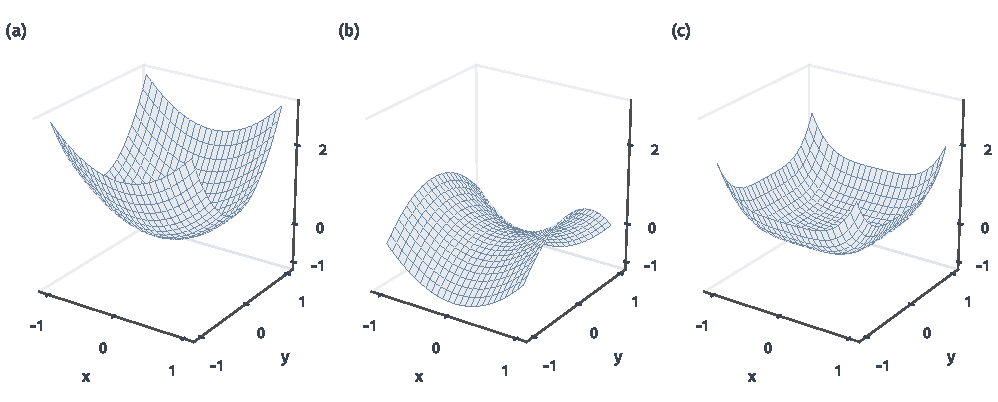
\includegraphics[width=169.0mm]{figures/01-mathematical-preliminaries-upper/00-shared/matplotlib/chapter3-concept-processes/hessian-local-shapes.pdf}
 \caption{同一$[-1,1]^2$范围和纵轴尺度下，三面分别为$x^2+2y^2$、$x^2-y^2$、$x^4+y^4$。原点的Hessian依次为正定、不定、零矩阵；前两者给严格极小与鞍点，第三者虽严格极小却不能由正定判据推出。零Hessian也可能没有极值，例如前述$x^3$，故退化不是一种确定分类。}
 \label{fig:analysis-process-hessian-local-shapes}
\end{figure*}

\FloatBarrier

\subsection{多元向量值函数的微分}

前面每个输入只产生一个实数。现在固定$F:U\subseteq\mathbb R^d\to\mathbb R^m$，同一输入同时产生$m$个输出分量。例如极坐标映射$(r,\theta)\mapsto(r\cos\theta,r\sin\theta)$把两个参数变成平面上的点；神经网络的一层把输入向量变成另一个向量；参数曲线（$d=1$）与参数曲面（$d=2$、$m=3$）也是这种映射的特殊情况。
此时要问的是：输入稍作改变，输出点整体怎样移动。有限个输出可以逐分量检查，但每个分量的输入仍要整体扰动，不能以坐标切片代替各分量的全微分。

\subsubsection{向量值函数及其极限与连续性}

向量值函数由它的全部输出分量确定，因此按分量书写。
\begin{definition}[多元向量值函数]
\label{def:multivariable-vector-function}
映射$F:U\subseteq\mathbb R^d\to\mathbb R^m$称为多元向量值函数，写作$F=(F_1,\ldots,F_m)^\top$，其中每个$F_i:U\to\mathbb R$为多元标量函数。
\end{definition}
向量值函数的极限与连续性使用输出欧氏距离$\lVert F(\bm x)-\bm b\rVert_2$，即要求输出点整体接近$\bm b$。
对有限个输出，$F(\bm x)\to\bm b$等价于每个分量$F_i(\bm x)\to b_i$，$F$在一点连续也等价于每个$F_i$在该点连续，因为
\[
 \max_i|F_i(\bm x)-b_i|\leq\lVert F(\bm x)-\bm b\rVert_2
 \leq\sqrt m\max_i|F_i(\bm x)-b_i|.
\]
左侧不等式说明整体接近时每个分量都接近；右侧说明每个分量都接近到$\varepsilon/\sqrt m$以内时，整体误差小于$\varepsilon$。
这里分解的是输出分量，区别于只沿某些输入坐标检查的切片：每个分量$F_i$仍须在全部输入方向上联合趋近。

\subsubsection{微分与Jacobian矩阵}

标量输出的全微分是到实数的线性映射，也称线性泛函；向量输出的全微分则要把输入扰动映射为$m$维输出扰动。
有限维线性映射由矩阵表示，矩阵的每一行记录一个输出分量的系数。
\begin{definition}[向量值函数的微分]
\label{def:multivariable-vector-differential}
设$U$开，$F:U\to\mathbb R^m$，$\bm a\in U$。若存在矩阵$\bm J_F(\bm a)\in\mathbb R^{m\times d}$，使
\begin{equation}
 F(\bm a+\bm h)=F(\bm a)+\bm J_F(\bm a)\bm h+o(\lVert\bm h\rVert_2),
\label{eq:analysis-jacobian-linearization}
\end{equation}
则称$F$在$\bm a$处可微，余项按输出欧氏范数理解。
其微分为$\mathrm dF_{\bm a}(\bm h)=\bm J_F(\bm a)\bm h$，其中$\bm J_F$称为\term{Jacobian矩阵}（Jacobian matrix），第$i,j$个元素为$\partial_jF_i$。
\end{definition}
向量值函数可微当且仅当每个输出分量$F_i$可微：正向可从向量余项取第$i$个分量，得到$F_i$的标量展开；反向则将有限个分量的$o(\lVert\bm h\rVert_2)$余项用欧氏范数合并，合并后仍是$o(\lVert\bm h\rVert_2)$。
因此Jacobian的第$i$行是标量分量梯度$\nabla F_i^\top$；$m=1$时Jacobian是梯度的转置，而不是梯度列向量本身。
$C^k$向量值函数指所有输出分量都属于$C^k$。

\paragraph{Jacobian矩阵的几何意义}
按列看Jacobian，第$j$列
\[
 \bm J_F(\bm a)\bm e_j=(\partial_jF_1,\ldots,\partial_jF_m)^\top
\]
表示：只把第$j$个输入增加一个很小的量$t$时，输出点大约沿这个向量移动$t$倍。一般扰动$\bm h=\sum_jh_j\bm e_j$的一阶效果就是这些列按$h_j$加权求和。
对$d=m=2$，这给出局部伸缩的图像：以$\bm a$为角、边长为$\varepsilon$的小正方形，由$\varepsilon\bm e_1,\varepsilon\bm e_2$张成，它的像近似是由$\varepsilon\bm J_F\bm e_1,\varepsilon\bm J_F\bm e_2$张成的平行四边形。行列式的绝对值是线性映射对面积的缩放倍数（第~\ref{sec:prelim-determinants}节），所以像的面积约为$|\det\bm J_F(\bm a)|\varepsilon^2$；行列式的符号说明局部是否翻转了定向。

极坐标映射给出这种局部伸缩的一个具体例子。
\begin{example}[极坐标映射的Jacobian矩阵]
\label{ex:multivariable-polar-jacobian}
考虑极坐标映射
\[
 P(r,\theta)=(r\cos\theta,r\sin\theta)^\top.
\]
逐个输出分量求偏导，得到
\[
 \bm J_P(r,\theta)=\begin{bmatrix}\cos\theta&-r\sin\theta\\ \sin\theta&r\cos\theta\end{bmatrix},
 \qquad \det\bm J_P=r\cos^2\theta+r\sin^2\theta=r.
\]
第一列是单位径向向量：$r$增加$\mathrm dr$，点沿射线向外移动$\mathrm dr$。第二列长度为$r$、沿圆周切向：$\theta$增加$\mathrm d\theta$，点沿半径为$r$的圆移动约$r\,\mathrm d\theta$。因此参数平面中面积为$\mathrm dr\,\mathrm d\theta$的小矩形，变成面积约为$r\,\mathrm dr\,\mathrm d\theta$的小扇形块。
\end{example}

离原点越远，同样的角度增量扫过的弧越长，面积放大越多；第~\ref{sec:multivariable-change-variables}节的区域积分换元正是用这个倍数校正面积。

图~\ref{fig:analysis-process-jacobian-grid-cell}把一个非线性映射的线性近似画成小网格块的变化。图中$\det J_T(a)=1\times0.6-0.25\times0.3=0.525$，绿色小方块的像面积约为原面积的一半。
\begin{figure*}[!htbp]
 \centering
 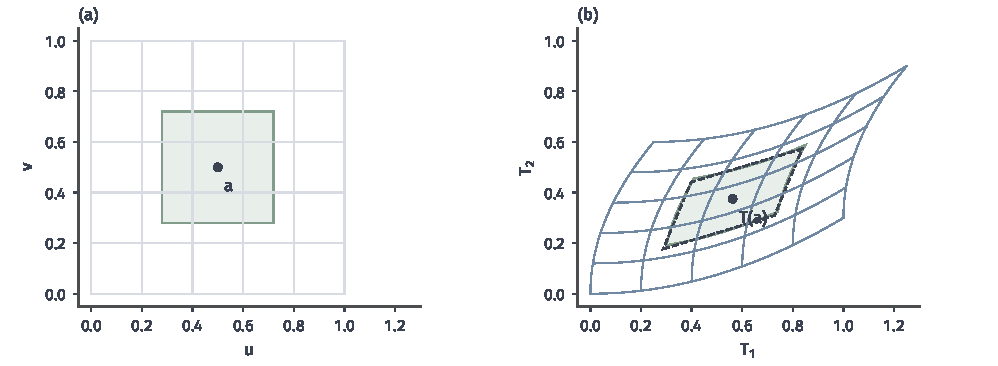
\includegraphics[width=169.0mm]{figures/01-mathematical-preliminaries-upper/00-shared/matplotlib/chapter3-concept-processes/jacobian-grid-cell.pdf}
 \caption{取$T(u,v)=(u+v^2/4,\,0.6v+0.3u^2)$，$a=(0.5,0.5)$。(a) 输入网格及绿色小方块。(b) 非线性像为弯边块，黑虚线为$T(a)+J_T(a)(h,k)^\top$给出的平行四边形；$J_T(a)=\bigl[\begin{smallmatrix}1&0.25\\0.3&0.6\end{smallmatrix}\bigr]$。有限块不与线性像完全重合，缩小扰动后才由可微余项控制差异。}
 \label{fig:analysis-process-jacobian-grid-cell}
\end{figure*}

\paragraph{Jacobian矩阵的计算}
计算Jacobian矩阵时，每个输出先按标量函数求偏导，再按行排列；排好后可以核对输入、输出与矩阵形状是否一致。
例如$F(x,y)=(x^2+xy,y^2)^\top$的Jacobian为
\[
 \bm J_F(x,y)=\begin{bmatrix}2x+y&x\\0&2y\end{bmatrix}.
\]
在$(1,2)$处，它把扰动$(h,k)^\top$的一阶影响写成$(4h+k,4k)^\top$。两个输出分别占一行，两个输入分别占一列。

机器学习中一个常用的向量值映射，是把任意一组实数变成正数且总和为$1$的权重：先取指数，再除以共同的总和。
这就是$n$维\term{归一化指数映射}（softmax），分类模型常用它把各类别的得分变成概率。对正整数$n$和
$\bm{z}\in\mathbb{R}^n$，令
\[
  s_i(\bm{z})
  =
  \frac{e^{z_i}}{\sum_{k=1}^n e^{z_k}},
  \qquad i=1,\ldots,n.
\]
记分母为$Z=\sum_k e^{z_k}$，它对$z_j$的偏导数为$e^{z_j}$。对分子$e^{z_i}$求偏导，$i=j$时得$e^{z_i}$，$i\neq j$时得$0$，记为$\mathbb{I}\{i=j\}e^{z_i}$。商法则给出
\[
  \frac{\partial s_i}{\partial z_j}
  =
  \frac{\mathbb{I}\{i=j\}e^{z_i}Z-e^{z_i}e^{z_j}}{Z^2}
  =
  s_i\bigl(\mathbb{I}\{i=j\}-s_j\bigr).
\]
因此整个Jacobian矩阵为
\begin{equation}
  \bm{J}_{\bm{s}}(\bm{z})
  =
  \operatorname{diag}(\bm{s})-\bm{s}\bm{s}^{\top}.
\label{eq:analysis-softmax-jacobian}
\end{equation}
这里$\operatorname{diag}(\bm s)$表示以$s_1,\ldots,s_n$为对角元、其他元素为零的对角矩阵。

对角项$s_i(1-s_i)$为正，描述提高$z_i$对自身分量的影响；非对角项$-s_is_j$为负，来自共同分母：提高一个得分会压低其余归一化分量。每行元素之和为$s_i-s_i\sum_js_j=0$，这与给所有$z_i$同时加同一常数不改变输出相符：沿方向$(1,\ldots,1)^\top$的一阶变化为零。

在最简单的情形中，可以用数值核对式~\eqref{eq:analysis-softmax-jacobian}给出的线性近似。
\begin{example}[二维softmax的Jacobian矩阵]
\label{ex:multivariable-softmax-jacobian-check}
取$n=2$、$\bm z=\bm 0$，则$\bm s=(1/2,1/2)^\top$，由式~\eqref{eq:analysis-softmax-jacobian}，
\[
 \bm J_{\bm s}(\bm 0)
 =\begin{bmatrix}1/2&0\\0&1/2\end{bmatrix}-\begin{bmatrix}1/4&1/4\\1/4&1/4\end{bmatrix}
 =\begin{bmatrix}1/4&-1/4\\-1/4&1/4\end{bmatrix}.
\]
把$z_1$提高$0.1$，线性近似给出$\bm s$的增量约为
\[
 \bm J_{\bm s}(\bm 0)(0.1,0)^\top=(0.025,-0.025)^\top,
\]
即$s_1\approx0.525$、$s_2\approx0.475$。实际值为$s_1=e^{0.1}/(e^{0.1}+1)\approx0.52498$、$s_2\approx0.47502$。
\end{example}

线性近似与实际值只差约$2\times10^{-5}$，远小于输入改变量$0.1$；两个分量的增量一正一负、总和为零，与$s_1+s_2$恒为$1$相符。

\subsubsection{向量值函数的微分运算}
\label{sec:analysis-vector-chain-matrix-calculus}

运算法则以运算有定义为前提。输出形状相同的向量值函数可以相加、相减，任何向量值函数都可以数乘；复合则要求前一映射的输出落在后一映射的定义域内。
两个向量之间的乘法需要先指定含义（例如内积），本小节不讨论乘积法则。

\paragraph{和的微分}
若$F,H:U\to\mathbb R^m$在$\bm a$处可微，对每个输出分量分别使用标量的和法则，再把各分量的结果按行排回矩阵，得到
\[
 \bm J_{F+H}(\bm a)=\bm J_F(\bm a)+\bm J_H(\bm a).
\]
相加的输出形状以及两个Jacobian的形状必须分别一致。

\paragraph{差的微分}
在相同条件下，逐分量使用差法则，得到
\[
 \bm J_{F-H}(\bm a)=\bm J_F(\bm a)-\bm J_H(\bm a).
\]

\paragraph{数乘的微分}
对固定实数$c$，逐分量使用数乘法则，得到
\[
 \bm J_{cF}(\bm a)=c\bm J_F(\bm a).
\]

\paragraph{复合函数的链式法则}
复合映射$G\circ F$先用$F$把输入变成中间量，再用$G$把中间量变成输出。输入的小扰动$\bm h$先被$F$变成中间量的扰动，一阶上约为$\bm J_F\bm h$；这个扰动再被$G$变成输出扰动，一阶上约为$\bm J_G(\bm J_F\bm h)$。
因此复合微分按实际计算顺序组合，Jacobian的乘法次序由输入与输出维度决定。与一元情形一样，这项复合规则称为\term{链式法则}（chain rule）。
\begin{theorem}[向量值函数的链式法则]
\label{thm:multivariable-vector-chain-rule}
设$U\subseteq\mathbb R^d$、$V\subseteq\mathbb R^m$开，$F:U\to V$在$\bm a$处可微，$G:V\to\mathbb R^p$在$F(\bm a)$处可微，则$G\circ F$在$\bm a$处可微，且
\begin{equation}
 \bm J_{G\circ F}(\bm a)=\bm J_G(F(\bm a))\bm J_F(\bm a).
\label{eq:analysis-vector-chain-rule}
\end{equation}
\end{theorem}
\begin{proof}
记$\bm A=\bm J_F(\bm a)$、$\bm B=\bm J_G(F(\bm a))$。由$F$可微，中间量的增量为
\[
 \bm k=F(\bm a+\bm h)-F(\bm a)=\bm A\bm h+o(\lVert\bm h\rVert_2),
\]
故$\lVert\bm k\rVert_2\leq\lVert\bm A\bm h\rVert_2+o(\lVert\bm h\rVert_2)=O(\lVert\bm h\rVert_2)$：中间量的扰动与原扰动同阶。
代入$G$的一阶展开，
\[
 G(F(\bm a)+\bm k)-G(F(\bm a))=\bm B\bm k+o(\lVert\bm k\rVert_2)
 =\bm B\bm A\bm h+\bm B\,o(\lVert\bm h\rVert_2)+o(\lVert\bm k\rVert_2).
\]
右侧第二项中，矩阵$\bm B$至多把长度放大固定倍数，所以仍是$o(\lVert\bm h\rVert_2)$；第三项因$\lVert\bm k\rVert_2=O(\lVert\bm h\rVert_2)$也是$o(\lVert\bm h\rVert_2)$（$\bm k=\bm0$时外层余项为零）。
于是复合增量等于$\bm B\bm A\bm h$加上$o(\lVert\bm h\rVert_2)$，这正是复合函数的可微定义。
\end{proof}
式~\eqref{eq:analysis-vector-chain-rule}中的矩阵形状为$(p\times m)(m\times d)=p\times d$，反向相乘往往没有定义。
即使两个次序都有定义，矩阵乘法一般也不交换，不能按标量经验调换因子。
用局部伸缩的语言说：复合映射在一点附近的伸缩，等于两步伸缩依次作用；方阵情形下，行列式的乘法公式还给出面积缩放倍数相乘。

链式法则常用于这样的情形：先用向量值映射得到中间量，再把中间量变成一个标量，最后求这个标量对原输入的梯度。
\begin{example}[从中间向量求回复合目标的梯度]
\label{ex:analysis-chain-rule-calculation}
令
\[
  F(x_1,x_2)=(x_1^2,x_1x_2,x_2)^\top,
  \qquad \ell(\bm y)=\frac12(y_1^2+y_2^2+y_3^2).
\]
$F$从二维输入产生三维中间量，$\ell$再把三维中间量变成一个数，复合得到$L=\ell\circ F:\mathbb R^2\to\mathbb R$。
$\ell$的Jacobian是$1\times3$行向量$\nabla\ell(\bm y)^\top$，由链式法则，$L$的Jacobian为$\nabla\ell(F(\bm x))^\top\bm J_F(\bm x)$；转置后得到列向量梯度
\[
  \nabla L(\bm x)=\bm J_F(\bm x)^\top\nabla\ell\bigl(F(\bm x)\bigr).
\]
这里出现转置，是因为梯度按列向量书写，而链式法则中的$\ell$导数是行向量。本例中
\[
  \bm J_F=\begin{bmatrix}2x_1&0\\x_2&x_1\\0&1\end{bmatrix},
  \qquad \nabla\ell(\bm y)=\bm y.
\]
在$\bm x=(1,2)^\top$处，$\bm y=(1,2,2)^\top$，链式法则给出
\[
  \nabla L(1,2)
  =\begin{bmatrix}2&2&0\\0&1&1\end{bmatrix}
    \begin{bmatrix}1\\2\\2\end{bmatrix}
  =\begin{bmatrix}6\\4\end{bmatrix}.
\]
也可以把复合函数直接展开为
$L(x_1,x_2)=\tfrac12(x_1^4+x_1^2x_2^2+x_2^2)$，求偏导得到
$\nabla L=(2x_1^3+x_1x_2^2,\,x_1^2x_2+x_2)^\top$，在同一点仍为$(6,4)^\top$。
矩阵形状$(2\times3)(3\times1)=2\times1$也核对了梯度传递的次序。
\end{example}

两种计算处理同一个目标；链式形式保留了中间映射，可以分别复用各层的导数。

\subsubsection{向量增量的中值估计}

标量函数的中值公式在线段上找到一个点，用那里的梯度精确表示增量。向量值函数不能照搬：各输出分量的一元中值点可能不同，没有一个共同位置代表整个向量增量。
例如$F(t)=(\cos t,\sin t)^\top$在$[0,2\pi]$上走完一整圈，$F(2\pi)-F(0)=\bm 0$，但速度$F'(t)=(-\sin t,\cos t)^\top$长度恒为$1$，不存在$\tau$使$F(2\pi)-F(0)=2\pi F'(\tau)$。
因此改为只控制增量的长度：用线性映射的最大放大倍数估计有限变化。

\paragraph{算子范数}

对标量函数，导数的绝对值说明输入的小变化被放大多少倍。对向量输出，同一矩阵在不同方向上放大的倍数可能不同，取其中最大的一个代替绝对值。
\begin{definition}[欧氏诱导算子范数]
\label{def:analysis-induced-operator-norm}
对矩阵
$\bm{A}\in\mathbb{R}^{s\times r}$，由欧氏范数\term{诱导的算子范数}
（induced operator norm）定义为
\[
  \lVert\bm{A}\rVert_{\mathrm{op}}
  =
  \sup_{\bm{h}\neq\bm{0}}
  \frac{\lVert\bm{A}\bm{h}\rVert_2}{\lVert\bm{h}\rVert_2}
  =
  \sup_{\lVert\bm{h}\rVert_2=1}\lVert\bm{A}\bm{h}\rVert_2.
\]
\end{definition}
算子范数是线性映射对向量长度的最大放大倍数，定义立即给出
$\lVert\bm{A}\bm{h}\rVert_2
\leq\lVert\bm{A}\rVert_{\mathrm{op}}\lVert\bm{h}\rVert_2$。
计算算子范数时，先给出对全部单位向量成立的上界，再找出达到上界的方向。
\begin{example}[对角矩阵的算子范数]
\label{ex:multivariable-diagonal-operator-norm}
令$\bm A=\operatorname{diag}(2,1)$，它把第一坐标放大两倍、第二坐标保持不变。对单位向量$\bm h$，
\[
 \lVert\bm A\bm h\rVert_2^2=4h_1^2+h_2^2\leq4(h_1^2+h_2^2)=4,
\]
且$\bm h=\bm e_1$时取等号，故$\lVert\bm A\rVert_{\mathrm{op}}=2$。
\end{example}

示例~\ref{ex:multivariable-diagonal-operator-norm}的最大放大由第一坐标方向达到。旋转矩阵不改变任何向量的长度，算子范数为$1$。

用算子范数控制增量长度后，就不再需要各分量共用一个中值点；所需条件是$G$在含整条线段的开集上连续可微。
\begin{theorem}[向量值函数的中值估计]
\label{thm:multivariable-vector-mean-value}
设$U\subseteq\mathbb R^r$开，$G:U\to\mathbb R^s$连续可微，且$[\bm y',\bm y]\subset U$，则
\begin{equation}
  \begin{aligned}
  \lVert G(\bm{y})-G(\bm{y}')\rVert_2
  &\leq
  \sup_{0\leq t\leq1}
  \left\lVert
    \bm{D}G\bigl(\bm{y}'+t(\bm{y}-\bm{y}')\bigr)
  \right\rVert_{\mathrm{op}}
  \lVert\bm{y}-\bm{y}'\rVert_2.
  \end{aligned}
\label{eq:analysis-operator-mean-value-bound}
\end{equation}
其中$\bm DG=\bm J_G$，即$G$的Jacobian矩阵。
\end{theorem}
\begin{proof}
思路是把向量增量投影到它自己的方向上，变成一个标量函数的增量，再对标量函数用中值定理。若$\bm u=G(\bm y)-G(\bm y')\neq\bm0$，
取单位向量$\bm v=\bm u/\lVert\bm u\rVert_2$，并沿线段定义标量函数
$\phi(t)=\bm v^\top G(\bm y'+t(\bm y-\bm y'))$。
由链式法则，$\phi'(t)=\bm v^\top\bm DG(\bm y'+t(\bm y-\bm y'))(\bm y-\bm y')$；中值定理给出某个$\tau\in(0,1)$，使
\[
 \lVert\bm u\rVert_2
 =\bm v^\top\bm u
 =\phi(1)-\phi(0)
 =\bm v^\top\bm DG(\bm y'+\tau(\bm y-\bm y'))(\bm y-\bm y').
\]
对右侧先用内积不等式并注意$\lVert\bm v\rVert_2=1$，再用算子范数的上界，便得到式~\eqref{eq:analysis-operator-mean-value-bound}；
$\bm u=\bm0$时该界直接成立。
\end{proof}
若定义域为凸开集，且Jacobian的算子范数在全域不超过同一个有限常数$L$，则由式~\eqref{eq:analysis-operator-mean-value-bound}，$G$以$L$为Lipschitz常数：任意两点的像之间的距离至多是原距离的$L$倍。在局部球上使用同样的界，就得到局部版本。
特别地，若Jacobian的算子范数在某个球内不超过一个常数$L<1$，映射就在球内严格缩小任意两点间的距离，称为压缩。第~\ref{sec:analysis-implicit-parameter-integral}节证明隐函数定理时，将用这一条件和几何级数的尾和控制迭代。

\subsection{矩阵自变量函数的微分}

本小节的定义域$\mathcal U$均为全矩阵空间$\mathbb R^{m\times n}$中的开集，基点$\bm X\in\mathcal U$；因此全部充分小的同形扰动都允许使用。
机器学习中的参数常排成矩阵，例如线性层的权重或协方差矩阵，损失是它们的标量函数，求逆、相乘等运算又产生矩阵输出。原则上可以把矩阵拉直成长向量，再用前面的结论；但保留矩阵形状，能让乘法次序与迹的结构更清楚，结果也能直接写成矩阵表达式。

$m\times n$矩阵输入可以看成$mn$个实数坐标，$r\times s$矩阵输出可以看成$rs$个实数分量，因此可微性仍是“扰动的一阶变化由线性映射给出”；只是扰动用Frobenius范数度量，线性映射的输入与输出都保留矩阵形状。
第~\ref{sec:prelim-matrix-trace}节已定义Frobenius内积与范数，满足$\langle\bm A,\bm B\rangle_F=\operatorname{tr}(\bm A^\top\bm B)=\sum_{i,j}A_{i,j}B_{i,j}$，即把两个矩阵对应元素相乘再求和，也就是拉直后的向量内积。

\paragraph{微分的定义}
设$\Phi:\mathcal U\to\mathbb R^{r\times s}$。若存在矩阵空间之间的线性映射$\mathrm d\Phi_{\bm X}:\mathbb R^{m\times n}\to\mathbb R^{r\times s}$，使
\[
 \Phi(\bm X+\bm H)=\Phi(\bm X)+\mathrm d\Phi_{\bm X}(\bm H)+o(\lVert\bm H\rVert_F),
\]
余项按输出的Frobenius范数度量，则称$\Phi$在$\bm X$处可微，$\mathrm d\Phi_{\bm X}$为其微分。这就是向量值可微性按矩阵形状重排后的写法：Frobenius范数正是拉直后向量的欧氏范数。

计算时常写$\mathrm d\Phi=\mathrm d\Phi_{\bm X}(\mathrm d\bm X)$，用乘积法则展开后保留乘法次序。例如$\mathrm d(\bm A\bm X\bm B)=\bm A(\mathrm d\bm X)\bm B$，扰动夹在中间的位置不能移动。
又如$\Phi(\bm X)=\bm X^2=\bm X\bm X$，展开得$(\bm X+\bm H)(\bm X+\bm H)=\bm X^2+\bm H\bm X+\bm X\bm H+\bm H^2$。其中$\lVert\bm H^2\rVert_F\leq\lVert\bm H\rVert_F^2$是高阶项，故$\mathrm d(\bm X^2)=(\mathrm d\bm X)\bm X+\bm X(\mathrm d\bm X)$；只有$\bm X$与扰动交换时，才能写成$2\bm X\,\mathrm d\bm X$。

\paragraph{标量输出与矩阵梯度}
输出为标量（$r=s=1$）时，线性映射$\mathrm df_{\bm X}$可以用一个同形矩阵与扰动的Frobenius内积表示，这个矩阵就是梯度。这与向量情形$\mathrm df=\nabla f^\top\mathrm d\bm x$完全对应。
\begin{definition}[矩阵标量函数的梯度]
\label{def:multivariable-matrix-scalar-gradient}
设$f:\mathcal U\to\mathbb R$在$\bm X$处可微。唯一满足
\begin{equation}
 \mathrm df_{\bm X}(\bm H)=\langle\nabla_{\bm X}f,\bm H\rangle_F
 =\operatorname{tr}\bigl((\nabla_{\bm X}f)^\top\bm H\bigr)
\label{eq:analysis-matrix-gradient-definition}
\end{equation}
的同形矩阵$\nabla_{\bm X}f\in\mathbb R^{m\times n}$称为矩阵梯度。
\end{definition}
取只有第$(i,j)$个元素为$1$的扰动$\bm H$，右侧内积只剩$\nabla_{\bm X}f$的第$(i,j)$个元素，左侧是对$X_{i,j}$的偏导数。所以矩阵梯度的各元素就是对相应矩阵坐标的偏导数，唯一性也由此得到。与向量梯度一样，$\nabla_{\bm X}f$指出使$f$增加最快的扰动方向。

求梯度时，先用乘积法则展开微分，再利用迹的循环移位把扰动移到末端，写成$\operatorname{tr}(\bm G^\top\mathrm d\bm X)$的形式，便读出$\nabla_{\bm X}f=\bm G$。乘积形状相容时，
\[
 \operatorname{tr}(\bm A\bm B)=\operatorname{tr}(\bm B\bm A),\qquad
 \operatorname{tr}(\bm A\bm B\bm C)=\operatorname{tr}(\bm B\bm C\bm A).
\]
这里循环移动的是整个因子，不能任意交换相邻矩阵。标量等于自己的迹，所以任何标量表达式都可以放进迹中再移位。
\begin{example}[双线性函数的矩阵梯度]
\label{ex:multivariable-bilinear-matrix-gradient}
对固定向量$\bm a\in\mathbb R^m$、$\bm b\in\mathbb R^n$，令$f(\bm W)=\bm a^\top\bm W\bm b$。它对$\bm W$线性，微分为$\mathrm df=\bm a^\top(\mathrm d\bm W)\bm b$。把这个标量写成迹并循环移位，
\[
 \mathrm df=\operatorname{tr}\bigl(\bm a^\top(\mathrm d\bm W)\bm b\bigr)=\operatorname{tr}\bigl(\bm b\bm a^\top\mathrm d\bm W\bigr)
 =\operatorname{tr}\bigl((\bm a\bm b^\top)^\top\mathrm d\bm W\bigr),
\]
于是$\nabla_{\bm W}f=\bm a\bm b^\top$。逐元素核对：$f=\sum_{k,l}a_kW_{k,l}b_l$，对$W_{i,j}$的偏导数是$a_ib_j$，正是$\bm a\bm b^\top$的第$(i,j)$个元素。
\end{example}

矩阵梯度的唯一性使用了全部矩阵方向。若把定义域限制在对称矩阵等子空间上，允许的扰动变少，满足式~\eqref{eq:analysis-matrix-gradient-definition}的矩阵不再唯一，还需另行说明所用的内积与允许方向。
矩阵输出时没有这样的单个梯度矩阵，只能保留线性映射$\mathrm d\Phi_{\bm X}$本身。以下依次计算迹、行列式与对数行列式这三个标量输出函数的微分，最后计算矩阵输出的逆矩阵。

\paragraph{迹函数的微分}
线性迹函数已经符合定义，可以直接读出梯度。对固定的$\bm{A}\in\mathbb{R}^{m\times n}$，令$f(\bm{X})=\operatorname{tr}(\bm{A}^{\top}\bm{X})=\sum_{i,j}A_{i,j}X_{i,j}$。由于$f$线性，$f(\bm X+\bm H)-f(\bm X)=\operatorname{tr}(\bm A^\top\bm H)$，没有余项，微分已经是式~\eqref{eq:analysis-matrix-gradient-definition}的形式，所以
\begin{equation}
  \nabla_{\bm{X}}\operatorname{tr}(\bm{A}^{\top}\bm{X})
  =\bm{A}.
\label{eq:analysis-trace-linear-gradient}
\end{equation}
这与向量情形$\nabla_{\bm x}(\bm a^\top\bm x)=\bm a$对应，常用于从迹表达式中读出梯度。

\paragraph{行列式的微分}
行列式把方阵映为一个实数，它是线性映射对体积的缩放倍数（第~\ref{sec:prelim-determinants}节）。这里要问：矩阵稍作扰动，体积缩放倍数怎样变化。先在最简单的基点$\bm X=\bm I$处计算。
\begin{example}[单位矩阵附近行列式的一阶变化]
\label{ex:multivariable-determinant-near-identity}
取$\bm H=\operatorname{diag}(\varepsilon_1,\varepsilon_2)$，则
\[
 \det(\bm I+\bm H)=(1+\varepsilon_1)(1+\varepsilon_2)=1+\varepsilon_1+\varepsilon_2+\varepsilon_1\varepsilon_2,
\]
一阶变化是$\varepsilon_1+\varepsilon_2=\operatorname{tr}\bm H$。若扰动只在非对角位置，例如$\bm H=\begin{bmatrix}0&\varepsilon\\0&0\end{bmatrix}$，则$\det(\bm I+\bm H)=1$，面积不变，而$\operatorname{tr}\bm H=0$。
\end{example}

两个方向各拉长一点时，面积的相对增量一阶上是两个伸长率之和；剪切扰动不改变面积，迹也为零。两种情形中，一阶变化都等于扰动的迹。

一般情形设$\bm X\in\mathbb R^{d\times d}$可逆，以便用行列式的乘法公式把扰动从行列式中分离出来：
\[
 \det(\bm X+\bm H)=\det(\bm X)\det(\bm I+\bm X^{-1}\bm H).
\]
记$\bm B=\bm X^{-1}\bm H$。按第~\ref{sec:prelim-determinants}节的排列展开，$\det(\bm I+\bm B)$是$\bm B$的元素的多项式。恒等排列给出$\prod_i(1+B_{i,i})=1+\operatorname{tr}\bm B+(\text{二次及以上项})$；非恒等排列至少改变两个位置，每个改变的位置只能选到$\bm B$的非对角元，因而只贡献二次及以上项。于是
\[
 \det(\bm I+\bm B)=1+\operatorname{tr}\bm B+O(\lVert\bm B\rVert_F^2).
\]
又$\lVert\bm B\rVert_F\leq\lVert\bm X^{-1}\rVert_F\lVert\bm H\rVert_F$，所以余项对一切小扰动$\bm H$统一为$O(\lVert\bm H\rVert_F^2)$；这保证得到的是全微分，而不只是固定方向上的导数。代回$\bm B=\bm X^{-1}\bm H$，便得到Jacobi行列式公式的一阶形式
\[
 \mathrm{d}\det\bm{X}=\det(\bm{X})\operatorname{tr}(\bm{X}^{-1}\mathrm{d}\bm{X}).
\]
它说明体积缩放倍数的相对变化$\mathrm d\det\bm X/\det\bm X$等于$\operatorname{tr}(\bm X^{-1}\mathrm d\bm X)$；$\bm X=\bm I$时回到示例~\ref{ex:multivariable-determinant-near-identity}中的$\operatorname{tr}\bm H$。

\paragraph{对数行列式的微分}
实数对数还要求$\det\bm X>0$，满足这一条件的矩阵组成开集，对数在其上与行列式复合。对上面的微分应用标量对数的链式法则，$\mathrm d\log u=\mathrm du/u$，得到
\begin{equation}
  \mathrm{d}\log\det\bm{X}
  =
  \operatorname{tr}(\bm{X}^{-1}\mathrm{d}\bm{X}),
  \qquad
  \nabla_{\bm{X}}\log\det\bm{X}
  =
  \bm{X}^{-\top}.
\label{eq:analysis-logdet-gradient}
\end{equation}
第二式由$\operatorname{tr}(\bm X^{-1}\mathrm d\bm X)=\operatorname{tr}\bigl((\bm X^{-\top})^\top\mathrm d\bm X\bigr)$对照式~\eqref{eq:analysis-matrix-gradient-definition}读出。
若$\bm X$还对称，则$\bm{X}^{-\top}=\bm{X}^{-1}$；一般情形应保留转置。$1\times1$时它回到$(\log x)'=1/x$。
这些计算都先找出扰动的一阶项，再用迹内积读出梯度；乘积次序与行列式展开决定了哪些变形成立。

\paragraph{逆矩阵的微分}
求逆映射的输入与输出都是方阵，属于矩阵输出的情形。逆矩阵与行列式非零的关系已在第~\ref{sec:prelim-inverse-matrices}节及第~\ref{sec:prelim-determinants}节建立。
计算分两步：先确认可微，再对乘法恒等式取微分。
第~\ref{sec:prelim-determinants}节的代数余子式公式把逆矩阵的各元素写成多项式与$\det\bm X$之比。
因此在$\det\bm X\neq0$的开集内，每个元素都是分母非零的有理函数，连续可微，逆映射也连续可微。
确认可微性后，对恒等式$\bm{X}\bm{X}^{-1}=\bm{I}$两侧取微分，左侧用乘积法则，右侧是常矩阵，得到
\[
 (\mathrm{d}\bm{X})\bm{X}^{-1}+\bm{X}\,\mathrm{d}(\bm{X}^{-1})=\bm{0}.
\]
左乘$\bm{X}^{-1}$后得到
\begin{equation}
  \mathrm{d}(\bm{X}^{-1})
  =
  -\bm{X}^{-1}(\mathrm{d}\bm{X})\bm{X}^{-1}.
\label{eq:analysis-inverse-differential}
\end{equation}
$1\times1$时这就是$(1/x)'=-1/x^2$。两个$\bm{X}^{-1}$位于扰动两侧，不能合并成$-\bm{X}^{-2}\mathrm{d}\bm{X}$，因为$\mathrm{d}\bm{X}$未必与$\bm{X}^{-1}$交换。
取一个对角矩阵和一个非对角扰动，就能看出两种写法的差别。
\begin{example}[逆矩阵微分中的乘法次序]
\label{ex:analysis-noncommuting-inverse-differential}
取$\bm X=\operatorname{diag}(2,1)$，扰动方向
$\bm E=\begin{bmatrix}0&1\\1&0\end{bmatrix}$。由式~\eqref{eq:analysis-inverse-differential}，沿$\bm X+t\bm E$求逆矩阵在$t=0$处的导数为
\[
 -\bm X^{-1}\bm E\bm X^{-1}
 =\begin{bmatrix}0&-1/2\\-1/2&0\end{bmatrix}.
\]
若照搬标量规则而写成$-\bm X^{-2}\bm E$，会得到
$\begin{bmatrix}0&-1/4\\-1&0\end{bmatrix}$。
直接核对：$(\bm X+t\bm E)^{-1}=\frac1{2-t^2}\begin{bmatrix}1&-t\\-t&2\end{bmatrix}$，在$t=0$处对$t$求导，非对角元为$-1/2$，对角元导数为$0$，与第一种结果一致。
\end{example}

错误写法连对称性都丢失了。路径$\bm X+t\bm E$在$t=0$附近由对称可逆矩阵组成，它们的逆也对称，所以导数必须对称；这一结构检查能直接发现错误。矩阵变量沿给定方向微分时，夹在扰动两侧的逆矩阵不能随意移到同一侧。

\subsection{隐函数与反函数}
\label{sec:analysis-implicit-parameter-integral}

前面对已给定的映射求微分；这里改变问题，先给定一组方程，再判断它是否在基点附近确定唯一的函数。
实际问题中，变量之间常由约束联系，而不是由显式公式给出：单位圆上的点满足$x^2+y^2=1$，物理系统的平衡状态满足力的平衡方程，模型训练的最优参数满足梯度为零。我们想知道，当一部分变量（参数）稍作改变时，其余变量（未知量）是否随之唯一地、光滑地改变，以及变化率是多少。
一般方程组用向量值映射表示。方程个数与待解变量个数相同时，关于待解变量的方阵Jacobian是否可逆，决定了能否在局部解出这些变量。

\subsubsection{隐函数的定义}

显式函数直接给出输出，例如$y=\sqrt x$。关系$F(x,y)=0$则没有直接告诉我们给定$x$时$y$取什么值：可能有多个$y$满足方程，也可能一个都没有。
设$(a,b)$满足$F(a,b)=0$。若存在$a$附近的区间$I$、$b$附近的区间$J$和函数$\varphi:I\to J$，使得对$I\times J$中的点，$F(x,y)=0$成立恰好当$y=\varphi(x)$，就称方程在$(a,b)$附近确定了一个\term{隐函数}（implicit function）$y=\varphi(x)$。换句话说，只看$(a,b)$附近的小矩形，方程的解集恰是一个函数的图像。
隐函数研究的第一步是说明局部解分支存在且唯一，然后才对这条分支求导。

同一个方程在不同的点附近，可能确定隐函数，也可能不确定。
\begin{example}[单位圆附近的隐函数]
\label{ex:multivariable-implicit-circle}
考虑单位圆$x^2+y^2-1=0$。在$(0,1)$附近，解集是上半圆$y=\sqrt{1-x^2}$的一段；在$(0,-1)$附近则是下半圆$y=-\sqrt{1-x^2}$的一段，两处都确定了隐函数。
但在$(1,0)$附近，每个略小于$1$的$x$对应上下两个解，略大于$1$的$x$没有解；无论矩形多小，解集都不是关于$x$的函数图像。此处圆的切线是竖直的。
\end{example}

解集分成几支时，还要指定从哪一个解出发。
\begin{example}[方程$y^2=x$的两支解]
\label{ex:multivariable-implicit-parabola-branches}
方程$y^2-x=0$在$x>0$时有正、负两支解$y=\pm\sqrt x$。固定其中一个非零解，例如$(1,1)$，可以在它附近选出唯一的正支。
但在$(0,0)$处两支相交，负$x$侧又没有实数解，因此不存在定义在含$0$的开区间上的解函数。
\end{example}

两个例子中不能局部解出$y$的点，都满足$\partial F/\partial y=2y=0$：单位圆在$(1,0)$处如此，$y^2-x$在$(0,0)$处也如此。这正是定理~\ref{thm:analysis-implicit-function}所要求的可逆性失效的地方。因此，局部选解既要指定起始解，也要核对关于待解变量的导数。

图~\ref{fig:vol1-add-implicit-branches}说明“局部唯一”怎样排除另一支解。在$(1,1)$附近只保留正支即可；在原点处，两支相交且负$x$没有实数解，不能用同样的方式局部选出可微的解。
\begin{figure}[!htb]
  \centering
  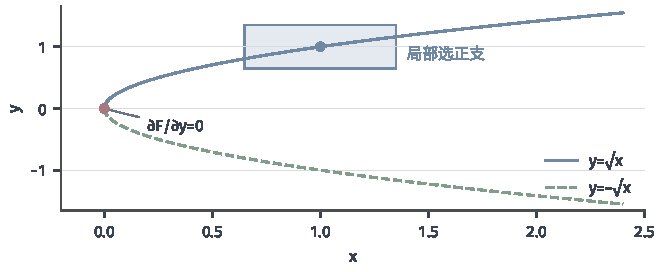
\includegraphics[width=112mm]{figures/01-mathematical-preliminaries-upper/00-shared/matplotlib/mathematical-language-combinatorics-analysis-optimization-comprehension-additions/implicit-branches.pdf}
  \caption{方程$F(x,y)=y^2-x=0$的两支实数解。浅蓝矩形围住$(1,1)$，在该矩形内每个允许的$x$只有正支解，且$F_y=2y\neq0$；红点处$F_y=0$，两支相交。两支解满足同一方程，选定起始解与邻域才确定隐函数分支。}
  \label{fig:vol1-add-implicit-branches}
\end{figure}
\FloatBarrier


\subsubsection{隐函数的存在、唯一性与微分}

为什么条件是关于待解变量的导数可逆？先看线性方程。设$\bm x\in\mathbb R^p$为参数、$\bm y\in\mathbb R^m$为未知量，$\bm P\in\mathbb R^{m\times p}$、$\bm Q\in\mathbb R^{m\times m}$固定，方程$\bm P\bm x+\bm Q\bm y=\bm 0$有$m$个方程、$m$个未知量。当$\bm Q$可逆时，对每个$\bm x$都有唯一解$\bm y=-\bm Q^{-1}\bm P\bm x$；$\bm Q$不可逆时，解要么不存在，要么不唯一。

对非线性方程$F(\bm x,\bm y)=\bm 0$，可微性说明它在基点附近近似于线性方程
\[
 \bm D_{\bm x}F(\bm a,\bm b)(\bm x-\bm a)+\bm D_{\bm y}F(\bm a,\bm b)(\bm y-\bm b)\approx\bm 0,
\]
其中$\bm D_{\bm x}F$、$\bm D_{\bm y}F$分别是只对$\bm x$、只对$\bm y$的坐标求偏导排成的Jacobian块。隐函数定理断言：只要线性近似中$\bm Q=\bm D_{\bm y}F$可逆，非线性方程在局部也像线性方程一样有唯一解，而且解的导数就是线性解的系数$-\bm Q^{-1}\bm P$。

隐函数定理给出的是充分条件：先保证局部解存在且唯一，再保证解随参数连续可微。
可逆性只要求待解变量对应的方阵Jacobian可逆，并不要求整个带参数映射的Jacobian是方阵。
\begin{theorem}[隐函数定理]
\label{thm:analysis-implicit-function}
设$F:\mathbb{R}^p\times\mathbb{R}^m\to\mathbb{R}^m$在$(\bm{a},\bm{b})$的某个开邻域内连续可微，$F(\bm{a},\bm{b})=\bm{0}$，并且关于待解变量的Jacobian矩阵
\[
 \bm{D}_{\bm{y}}F(\bm{a},\bm{b})\in\mathbb{R}^{m\times m}
\]
可逆。则存在$\bm{a}$与$\bm{b}$的邻域$U,V$，以及唯一的连续可微函数
$\varphi:U\to V$，使$\varphi(\bm{a})=\bm{b}$，并且对所有
$(\bm{x},\bm{y})\in U\times V$都有
\[
  F(\bm{x},\bm{y})=\bm{0}
  \quad\Longleftrightarrow\quad
  \bm{y}=\varphi(\bm{x}).
\]
其Jacobian矩阵满足
\begin{equation}
  \bm{D}\varphi(\bm{x})
  =
  -
  \bigl[\bm{D}_{\bm{y}}F(\bm{x},\varphi(\bm{x}))\bigr]^{-1}
  \bm{D}_{\bm{x}}F(\bm{x},\varphi(\bm{x})).
\label{eq:analysis-implicit-derivative}
\end{equation}
\end{theorem}
若已知$\varphi$存在且可微，导数公式可以直接由链式法则得到：对恒等式$F(\bm x,\varphi(\bm x))=\bm 0$求导，得$\bm D_{\bm x}F+\bm D_{\bm y}F\,\bm D\varphi=\bm 0$，再左乘$(\bm D_{\bm y}F)^{-1}$。定理真正困难的部分是$\varphi$的存在、唯一与可微，形式求导不能替代这些步骤。

证明的思路是把解方程改写为反复修正的迭代。一元时，固定$x$，从$y_0=b$出发，用$y_{n+1}=y_n-F(x,y_n)/F_y(a,b)$不断修正：若$F(x,y_n)>0$且$F_y(a,b)>0$，就把$y$调小一点。这类似Newton法，只是斜率固定用基点处的值。若每次修正都使误差按固定比例缩小，迭代就收敛到唯一解。
证明分别检查三件事：修正映射是压缩；它不把点送出所考察的球；所得解随参数可微。
\begin{proof}
为证明定理~\ref{thm:analysis-implicit-function}的存在性，先把方程改写为局部压缩迭代。记
\[
 \bm{A}=\bm{D}_{\bm{y}}F(\bm{a},\bm{b}),
 \qquad
 T_{\bm{x}}(\bm{y})=\bm{y}-\bm{A}^{-1}F(\bm{x},\bm{y}).
\]
因为$\bm A^{-1}$可逆，$F(\bm{x},\bm{y})=\bm{0}$当且仅当$T_{\bm{x}}(\bm{y})=\bm{y}$，即$\bm y$是更新后保持不变的点，称为不动点。并且
\[
 \bm{D}_{\bm{y}}T_{\bm{x}}(\bm{y})=\bm{I}-\bm{A}^{-1}\bm{D}_{\bm{y}}F(\bm{x},\bm{y}),
\]
它在$(\bm{a},\bm{b})$处为零。由$F$的导数连续，这个矩阵的元素在基点附近都很小；又由Cauchy--Schwarz不等式，算子范数不超过Frobenius范数。因而可以选择闭球$B=\{\bm{y}:\lVert\bm{y}-\bm{b}\rVert_2\leq r\}$和$\bm{a}$的邻域$U$，使
\begin{equation}
  \sup_{\bm{x}\in U,\,\bm{y}\in B}
  \left\lVert
    \bm{D}_{\bm{y}}T_{\bm{x}}(\bm{y})
  \right\rVert_{\mathrm{op}}
  \leq q<1.
\label{eq:analysis-ift-uniform-contraction}
\end{equation}
沿$\bm{y}$方向使用式~\eqref{eq:analysis-operator-mean-value-bound}（球是凸集，球内线段不离开球）可知，每个
$T_{\bm{x}}$都把$B$内任意两点之间的距离缩小到原来的至多$q$倍。

还必须核对自映射，即$T_{\bm x}$不把$B$中的点送出$B$；否则迭代可能离开压缩成立的范围。因为$T_{\bm{a}}(\bm{b})=\bm{b}$且$T_{\bm{x}}(\bm{b})$关于$\bm{x}$连续，可进一步缩小$U$，使
\[
 \lVert T_{\bm{x}}(\bm{b})-\bm{b}\rVert_2\leq\frac{1-q}{2}r.
\]
于是对$\bm{y}\in B$，先用三角不等式拆开，再用压缩性，
\[
 \begin{aligned}
  \lVert T_{\bm{x}}(\bm{y})-\bm{b}\rVert_2
  &\leq
  \lVert T_{\bm{x}}(\bm{y})-T_{\bm{x}}(\bm{b})\rVert_2+\lVert T_{\bm{x}}(\bm{b})-\bm{b}\rVert_2\\
  &\leq
  q\lVert\bm{y}-\bm{b}\rVert_2+\frac{1-q}{2}r
  \leq
  \frac{1+q}{2}r
  <r.
 \end{aligned}
\]
所以$T_{\bm{x}}(B)$包含在$B$的内部$V$中。
固定$\bm x\in U$，从$\bm y_0=\bm b$出发，令$\bm y_{n+1}=T_{\bm x}(\bm y_n)$。
所有迭代项都留在$B$内，每一步的压缩使相邻差满足
$\lVert\bm y_{n+1}-\bm y_n\rVert_2\leq q\lVert\bm y_n-\bm y_{n-1}\rVert_2\leq\cdots\leq q^n\lVert\bm y_1-\bm y_0\rVert_2$。
增大$q$仍保留这个上界，因而可设$0<q<1$。对$m>n$，几何和给出
\[
 \lVert\bm y_m-\bm y_n\rVert_2
 \leq\sum_{j=n}^{m-1}\lVert\bm y_{j+1}-\bm y_j\rVert_2
 \leq\frac{q^n}{1-q}\lVert\bm y_1-\bm y_0\rVert_2\longrightarrow0.
\]
每个坐标都是实柯西列，所以该序列在有限维欧氏空间中收敛；闭性使极限仍在$B$内。
$T_{\bm x}$连续，在$\bm y_{n+1}=T_{\bm x}(\bm y_n)$中令$n\to\infty$，可得极限$\varphi(\bm x)$满足
$T_{\bm x}(\varphi(\bm x))=\varphi(\bm x)$，而$T_{\bm x}(B)\subset V$使它属于$V$。
若另有不动点$\bm z\in B$，则
$\lVert\bm z-\varphi(\bm x)\rVert_2=\lVert T_{\bm x}(\bm z)-T_{\bm x}(\varphi(\bm x))\rVert_2\leq q\lVert\bm z-\varphi(\bm x)\rVert_2$，
由$q<1$只能有$\bm z=\varphi(\bm x)$，所以这个不动点唯一。若
$(\bm{x},\bm{y})\in U\times V$且$F(\bm{x},\bm{y})=\bm{0}$，则$\bm{y}\in B$也是
$T_{\bm{x}}$的不动点，唯一性迫使$\bm{y}=\varphi(\bm{x})$。这证明了定理所述的局部
存在与零点集合的逐点唯一性。

还需说明所得解随参数连续可微。先证$\varphi$局部Lipschitz连续，即它不会随参数剧烈变化。把$U$进一步缩小为开球，并使
$\overline U\times B$包含在原定义域内；这个集合闭且有界，$T_{\bm x}(\bm y)$关于$\bm x$的导数$-\bm A^{-1}\bm D_{\bm x}F$各分量连续，
故有统一范数上界$L$。对$\bm x,\bm x'\in U$，
两点间的线段仍在$U$内，式~\eqref{eq:analysis-operator-mean-value-bound}
可用于$T_{\bm x}(\bm y)$的参数变化。利用两个不动点关系$\varphi(\bm x)=T_{\bm x}(\varphi(\bm x))$、$\varphi(\bm x')=T_{\bm x'}(\varphi(\bm x'))$，把差拆成“改变$\bm y$”与“改变$\bm x$”两步：
\[
 \begin{aligned}
 \lVert\varphi(\bm{x})-\varphi(\bm{x}')\rVert_2
 &\leq\lVert T_{\bm x}(\varphi(\bm x))-T_{\bm x}(\varphi(\bm x'))\rVert_2\\
 &\quad+\lVert T_{\bm x}(\varphi(\bm x'))-T_{\bm x'}(\varphi(\bm x'))\rVert_2\\
 &\leq q\lVert\varphi(\bm{x})-\varphi(\bm{x}')\rVert_2+L\lVert\bm{x}-\bm{x}'\rVert_2,
 \end{aligned}
\]
移项得到$\lVert\varphi(\bm x)-\varphi(\bm x')\rVert_2
\leq L\lVert\bm x-\bm x'\rVert_2/(1-q)$，
故$\varphi$局部Lipschitz连续。

再证可微。令$\bm{h}\to\bm{0}$并记$\bm{k}=\varphi(\bm{x}+\bm{h})-\varphi(\bm{x})$，前述界给出$\lVert\bm{k}\rVert_2=O(\lVert\bm{h}\rVert_2)$。两点都在解集上，所以
\[
 F(\bm{x}+\bm{h},\varphi(\bm{x})+\bm{k})-F(\bm{x},\varphi(\bm{x}))=\bm{0}.
\]
对左侧作联合扰动$(\bm h,\bm k)$的一阶展开，得到
\[
 \bm{D}_{\bm{x}}F\,\bm{h}+\bm{D}_{\bm{y}}F\,\bm{k}+o(\lVert\bm{h}\rVert_2)=\bm{0}.
\]
展开中的Jacobian均在$(\bm x,\varphi(\bm x))$处取值，联合扰动的余项
$o(\lVert(\bm h,\bm k)\rVert_2)$因$\lVert\bm k\rVert_2=O(\lVert\bm h\rVert_2)$
成为$o(\lVert\bm h\rVert_2)$。
基点的$\det\bm A\neq0$，行列式又是矩阵元素的连续函数，
所以邻域足够小时$\bm D_{\bm y}F$仍可逆。左乘它的逆，得到
\[
 \bm{k}=-(\bm{D}_{\bm{y}}F)^{-1}\bm{D}_{\bm{x}}F\,\bm{h}+o(\lVert\bm{h}\rVert_2).
\]
这证明$\varphi$可微并给出式~\eqref{eq:analysis-implicit-derivative}；右侧各Jacobian矩阵及矩阵求逆都连续，又保证$\bm{D}\varphi$连续。至此，隐函数定理中的存在、局部唯一与导数公式都已得到证明。
\end{proof}

\paragraph{隐函数的导数}

定理的证明已同时建立解分支的存在、唯一性、可微性及式~\eqref{eq:analysis-implicit-derivative}。计算时只需在选定分支上代入两个Jacobian。用示例~\ref{ex:multivariable-implicit-parabola-branches}和示例~\ref{ex:multivariable-implicit-circle}的方程，可以核对不同分支各自的变化率。

\begin{example}[隐函数分支的导数]
设$F(x,y)=y^2-x$，在$(1,1)$处有$F=0$、$F_y=2\neq0$。
隐函数定理保证$(1,1)$附近的解可以唯一写成$y=\varphi(x)$，且
\[
 \varphi'(x)=-\frac{F_x(x,\varphi(x))}{F_y(x,\varphi(x))}
 =\frac1{2\varphi(x)},\qquad \varphi'(1)=\frac12.
\]
直接选正支$\varphi(x)=\sqrt x$，求导同样得到$1/(2\sqrt x)$。
若在$(1,-1)$附近选负支，导数则为$-1/2$。

对单位圆$x^2+y^2=1$上半圆的一点$(x_0,y_0)$（$y_0>0$），同一公式给出$\varphi'(x_0)=-x_0/y_0$，不必先解出$y=\sqrt{1-x^2}$。
\end{example}

起始解不同，所追踪的函数也不同，导数公式要在选定分支上取值。单位圆的导数$-x_0/y_0$在$y_0\to0$时趋于无穷，与$(1,0)$处的竖直切线相符，也与示例~\ref{ex:multivariable-implicit-circle}中$(1,0)$附近不能把$y$解成$x$的函数相一致。

\subsubsection{反函数的存在与微分}

另一个常见问题是反求输入：已知映射$G$的输出$\bm y$，能否唯一确定产生它的输入$\bm x$，并且$\bm x$随$\bm y$光滑变化。例如由直角坐标$(x,y)$反求极坐标$(r,\theta)$。
线性映射$\bm y=\bm M\bm x$可逆当且仅当方阵$\bm M$可逆；非线性映射在一点附近近似于它的Jacobian，所以可以期待：Jacobian可逆时，映射在局部可逆。
把$G(\bm x)-\bm y=\bm 0$看成以输出为参数、输入为待解变量的一组方程，就能使用隐函数定理。
定理只给出两个邻域之间的逆映射，不断言$G$在整个定义域上单射。
\begin{theorem}[局部反函数定理]
\label{thm:multivariable-inverse-function}
设$U\subseteq\mathbb R^d$开，$G:U\to\mathbb R^d$连续可微，$\bm a\in U$，且$\bm J_G(\bm a)$可逆。
则存在$\bm a$的开邻域$U_0$与$G(\bm a)$的开邻域$V_0$，使$G:U_0\to V_0$为双射，逆映射连续可微，并满足
\[
 \bm J_{G^{-1}}(G(\bm x))=[\bm J_G(\bm x)]^{-1}
 \qquad(\bm x\in U_0).
\]
\end{theorem}
\begin{proof}
以输出$\bm y$为参数、原输入$\bm x$为待解变量，令$H(\bm y,\bm x)=G(\bm x)-\bm y$。
在$(G(\bm a),\bm a)$处，关于$\bm x$的Jacobian就是可逆的$\bm J_G(\bm a)$。隐函数定理给出开邻域$V_0$、$W$以及$C^1$映射$\varphi:V_0\to W$，使
\[
 G(\bm x)=\bm y\quad\Longleftrightarrow\quad\bm x=\varphi(\bm y)
 \qquad(\bm y\in V_0,\ \bm x\in W).
\]
将$W$缩小并重新选取$V_0$，可使$W\subset U$且$\bm J_G$在$W$内均可逆。
令$U_0=W\cap G^{-1}(V_0)$，它因$G$连续而为包含$\bm a$的开集。
每个$\bm y\in V_0$都有$G(\varphi(\bm y))=\bm y$，故$\varphi(\bm y)\in U_0$；反之，每个$\bm x\in U_0$都由上述唯一性满足$\varphi(G(\bm x))=\bm x$。
因此$G:U_0\to V_0$为双射，逆就是$C^1$映射$\varphi$。
对$G(\varphi(\bm y))=\bm y$使用链式法则，得到$\bm J_G(\varphi(\bm y))\bm J_\varphi(\bm y)=\bm I$，左乘逆矩阵便得到所述公式。
\end{proof}
公式说明，逆映射的局部伸缩恰好抵消原映射的局部伸缩。极坐标映射可以具体说明这一点。
\begin{example}[极坐标的局部反函数]
\label{ex:multivariable-polar-local-inverse}
对$P(r,\theta)=(r\cos\theta,r\sin\theta)^\top$，示例~\ref{ex:multivariable-polar-jacobian}算得$\det\bm J_P=r$，所以在$r>0$的每一点附近，都可以从$(x,y)$唯一、光滑地反求$(r,\theta)$。在$(r,\theta)=(2,\pi/2)$，即平面上的点$(0,2)$处，
\[
 \bm J_P=\begin{bmatrix}0&-2\\1&0\end{bmatrix},
 \qquad
 \bm J_{P^{-1}}(0,2)=\bm J_P^{-1}=\begin{bmatrix}0&1\\-1/2&0\end{bmatrix}.
\]
第一行说明$\mathrm dr=\mathrm dy$：在正上方的点，向上移动直接增大半径。第二行说明$\mathrm d\theta=-\mathrm dx/2$：向左移动使角度增大，且因为半径为$2$，角度变化只有水平位移的一半。
\end{example}

在原点$r=0$处，Jacobian行列式为零，所有$\theta$都映到同一点，确实无法反求$\theta$；这正是定理条件不满足的地方。

\paragraph{局部可逆与整体单射}

Jacobian处处可逆仍不保证映射在整个定义域上单射。
\begin{example}[Jacobian处处可逆而不单射]
\label{ex:multivariable-local-not-global-inverse}
考虑映射
\[
 g(u,v)=(e^u\cos v,e^u\sin v)^\top,\qquad (u,v)\in\mathbb R^2.
\]
它的Jacobian矩阵为
\[
 \bm J_g(u,v)=\begin{bmatrix}e^u\cos v&-e^u\sin v\\ e^u\sin v&e^u\cos v\end{bmatrix},
 \qquad \det\bm J_g=e^{2u}>0,
\]
处处可逆。但$(u,v)$与$(u,v+2\pi)$给出同一输出，$g$不是单射。
\end{example}

这个$g$就是半径取$e^u$的极坐标映射：在每一点附近可以反求，整个平面上的输入却绕着原点重复覆盖输出。

另一方面，存在连续逆也不保证逆可微：一元函数$x\mapsto x^3$全局单射，其逆$y\mapsto y^{1/3}$在$0$处没有有限导数；这正对应$x^3$在$0$处导数为零，定理条件不满足。使用局部反函数定理时，需要逐项检查邻域、可微性和Jacobian的可逆性。

\FloatBarrier

\section{区域积分}
\label{sec:multivariable-region-integration}

一块不均匀的金属薄片占据平面区域$D$，在点$(x,y)$附近每单位面积的质量为$\rho(x,y)$。
把$D$切成许多小块，每块的质量约等于块内某一点的密度乘这块的面积；把所有小块的质量相加，就得到总质量的近似值，小块切得越细，近似越准确。
空间物体的质量、带电体的总电荷也按同样方式累计，只是面积换成体积，面密度换成体密度或电荷密度。
这类问题中的被积函数都是多元标量函数$f:D\subseteq\mathbb R^d\to\mathbb R$：输入是一个位置的$d$个坐标，输出是该位置上一个待累计的数。

同一个积分还有两种常用读法。
若$f\geq0$定义在平面区域$D$上，积分等于以$D$为底、以$f$的图像为顶的立体的体积，这是一元积分“曲线下方面积”在高一维的对应。
把积分除以$D$的面积，所得的数是$f$在$D$上的平均值，例如一个地区的平均降雨量或一块薄板的平均温度。

第~\ref{sec:analysis-measurability-integration}节在实轴上用长度给小块赋权，再由简单函数逼近和绝对可积要求建立了勒贝格积分。
推广到$\mathbb R^d$时只需更换两样东西：小块的大小改用$d$维体积来度量，函数的输入改为$\mathbb R^d$中的点。
简单函数逼近、单调收敛和支配收敛的论证只用到“分层、相加、取极限”，不依赖输入有几个坐标，可以原样沿用。

定义建立以后，还要回答计算上的三个问题。
第一，能否先算每一条切片上的累计，再把各切片的结果累加，也就是把区域积分拆成逐个坐标的一元积分？答案取决于非负性或绝对可积性，它们保证两种累计次序给出同一个区域积分。
第二，圆盘、球体等区域在直角坐标下边界复杂，能否改用极坐标、球坐标描述？换坐标会放大或缩小每个小块的体积，需要用Jacobian行列式校正。
第三，被积函数依赖一个参数时，积分值怎样随参数变化，能否在积分号下求导？
本节先建立多维测度与区域积分，再依次讨论这三个问题。切片与坐标计算的更多例题可参考\scite{math-openstax-calculus3}。

\subsection{多维测度与乘积测度}
\label{sec:comb-multidimensional-product-measure}

区域积分首先要回答“一块区域有多大”。
实轴上的长度已经由勒贝格测度给出；平面上的面积、空间中的体积也需要同样精确的定义，否则无法给边界弯曲、带有无穷多个小洞或形状不规则的区域赋予大小。
本小节先把第~\ref{sec:comb-set-measurement}节的区间覆盖构造搬到$\mathbb R^d$，再说明把$\mathbb R^d$拆成$\mathbb R^p\times\mathbb R^q$（$d=p+q$）时，$d$维体积怎样由$p$维与$q$维的体积相乘得到。
后一点是第~\ref{sec:multivariable-iterated-integrals}节累次积分成立的测度基础。

\subsubsection{多维勒贝格测度}

\paragraph{坐标盒}

实轴上的构造从区间出发，因为区间的长度不需要另行定义。
$\mathbb R^d$中与区间对应的对象是各坐标方向上区间的笛卡尔积，称为坐标盒，例如
\[
 Q=\prod_{i=1}^d(a_i,b_i),\qquad a_i<b_i.
\]
平面上的坐标盒是各边平行于坐标轴的长方形，空间中的坐标盒是长方体。
坐标盒的体积规定为各边长之积$\operatorname{vol}(Q)=\prod_i(b_i-a_i)$，例如$(0,2)\times(0,3)$的面积为$6$。
这条规定推广了长方形面积公式，也与有限集合的计数规则$|A\times B|=|A||B|$一致：一个方向排$m$个单位格、另一个方向排$n$个单位格时，共有$mn$个单位格。
闭盒、半开盒与同端点开盒的体积相同；某一边长为零的退化盒，例如平面上的一条线段，体积为零。

\paragraph{多维勒贝格测度}

一维外测度用可数个区间覆盖集合，再取覆盖总长度的下确界。
把区间换成开坐标盒、把长度换成体积，就得到$\mathbb R^d$上的外测度
\[
 m_d^*(E)=\inf_{\substack{E\subseteq\bigcup_{n=1}^{\infty}Q_n\\
 Q_n\text{为开坐标盒}}}\sum_{n=1}^{\infty}\operatorname{vol}(Q_n),
\]
其中下确界取遍$E$的所有可数开盒覆盖。
直观上，这是用盒子从外侧包住$E$，看至少需要多少总体积。

按这个定义，线段和可数点集的面积都是零。
线段$[0,1]\times\{0\}$能被一个开盒$(-\varepsilon,1+\varepsilon)\times(-\varepsilon,\varepsilon)$覆盖，这个盒的面积$2\varepsilon(1+2\varepsilon)$可以任意小，所以线段的二维外测度为零：线段有长度，却没有面积。
把$\mathbb Q^2$的点排成一列，第$k$个点放进面积为$\varepsilon2^{-k}$的小盒，这些小盒的总面积不超过$\varepsilon$，因此$\mathbb Q^2$的二维外测度也为零，论证与实轴上可数集零测相同。

可测集仍沿用定义~\ref{def:analysis-lebesgue-measurable-set}的分割要求：若集合$A\subseteq\mathbb R^d$对每个测试集合$E\subseteq\mathbb R^d$满足
$m_d^*(E)=m_d^*(E\cap A)+m_d^*(E\setminus A)$，就称$A$为$d$维勒贝格可测集。
一维情形中关于外测度的可数次可加性、可测集族构成$\sigma$代数、测度的可数可加性以及零测集子集可测的论证，只用到覆盖、取下确界和分割这几种操作，没有用到区间只有一个方向，所以把区间换成盒以后可以逐步照搬。
于是$d$维勒贝格可测集组成$\sigma$代数$\mathcal L(\mathbb R^d)$；把$m_d^*$限制在$\mathcal L(\mathbb R^d)$上，得到$d$维勒贝格测度$m_d$，其中$m_1$就是第~\ref{sec:comb-set-measurement}节的$m$。
$m_d$是完备的，即零测集的子集都可测。
需要另作核对的只有$m_d(Q)=\operatorname{vol}(Q)$，即可数个盒的覆盖不会把一个盒的体积算小；它对应一维中“区间的外测度等于其长度”的论证，这里不再重复。

常用的集合都在这个可测范围内。
坐标半空间$\{\bm x:x_i\leq t\}$的可测性与一维半直线相同：把每个覆盖盒沿超平面$x_i=t$切成两块，两块的体积之和仍是原盒的体积；坐标盒由这类半空间经取补集和可数次交、并得到，因而也可测。
每个欧氏开集又都是其中有理端点开盒的可数并：对开集中的每一点，先取一个包含该点且完全落在开集内的开盒，再把端点向内调整为有理数，使盒仍包含该点；有理端点的盒只有可数个。
因此$\mathcal L(\mathbb R^d)$包含全部开集，从而包含由全部开集（等价地，由全部开盒）生成的Borel $\sigma$代数$\mathcal B(\mathbb R^d)$；由于$m_d$完备，勒贝格范围还包含Borel零测集的全部子集。

\paragraph{平移与伸缩}

把集合$E$平移一个向量$\bm a$，每个覆盖盒也随之平移，盒的边长不变，所以$m_d(E+\bm a)=m_d(E)$。
把集合按比例$c>0$伸缩为$cE=\{c\bm x:\bm x\in E\}$时，每个覆盖盒的每条边都乘$c$，体积乘$c^d$，而$E$的覆盖与$cE$的覆盖一一对应，因此
\[
 m_d(cE)=c^dm_d(E).
\]
这正是“长度按$c$倍、面积按$c^2$倍、体积按$c^3$倍变化”的精确形式。
例如平面圆环$\{1\leq\lVert\bm x\rVert_2<2\}$放大$2^k$倍后得到$\{2^k\leq\lVert\bm x\rVert_2<2^{k+1}\}$，面积变为原来的$4^k$倍；示例~\ref{ex:region-power-function-threshold}判别幂函数的可积性时会用到这个事实。
一般线性映射对体积的放大倍数是行列式的绝对值，留到第~\ref{sec:multivariable-change-variables}节讨论。

\subsubsection{乘积测度}

累次积分要把$\mathbb R^d$看成$\mathbb R^p\times\mathbb R^q$，先在$\mathbb R^q$方向累计，再在$\mathbb R^p$方向累计。
为此需要知道$d$维体积与$p$维、$q$维体积之间的关系。
对坐标盒，答案已经包含在定义里：$d$条边长之积等于前$p$条边长之积乘后$q$条边长之积。
还需要确认两件事：对一般的Borel集合$A\subseteq\mathbb R^p$与$B\subseteq\mathbb R^q$，乘积集合$A\times B$（下文称为矩形）的体积是否仍为$m_p(A)m_q(B)$；只规定矩形的体积，能否唯一确定其余集合的$d$维体积。

\paragraph{矩形赋值的乘法规则}

矩形上的乘法规则可以先在只有有限个格子的情形中看清。
\begin{example}[有限网格上的乘积权重]
\label{ex:region-finite-product-weights}
横向分为两列，权重（可以理解为两段的长度或两组点的总质量）分别为$1,2$；纵向分为两行，权重分别为$3,4$。
规定每个格子的联合权重等于所在列、行权重之积，四个格子的权重就是$1\cdot3=3$、$2\cdot3=6$、$1\cdot4=4$、$2\cdot4=8$。
逐格相加得到总量
\[
 3+6+4+8=21=(1+2)(3+4),
\]
右侧先把两侧权重各自相加再相乘，两侧相等正是有限分配律。
先求每一行的总量$3+6=9$、$4+8=12$再相加，或先求每一列的总量$3+4=7$、$6+8=14$再相加，也都得到$21$。
\end{example}

逐格、逐行、逐列三种求和次序给出同一个总量，这就是累次积分在有限情形中的样子。
图~\ref{fig:analysis-process-product-measure-grid}把列宽和行高分别按两侧权重画成比例，格子面积因而等于乘积权重。
乘法规则只描述一种特定的联合赋权方式，一般的二元分布不必由两侧权重相乘得到。

\begin{figure}[!htbp]
 \centering
 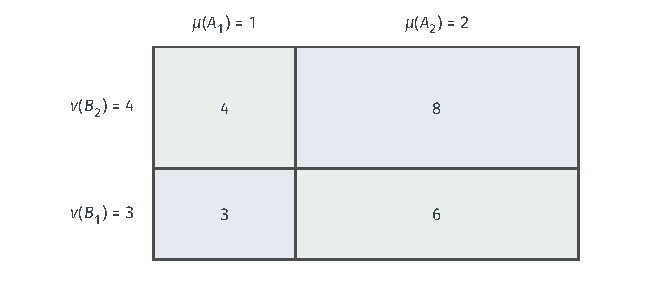
\includegraphics[width=112mm]{figures/01-mathematical-preliminaries-upper/00-shared/tikz/chapter3-concept-processes/product-measure-grid.pdf}
 \caption{两列的权重分别为$1,2$（图中记为$\mu(A_1),\mu(A_2)$），两行的权重分别为$3,4$（记为$\nu(B_1),\nu(B_2)$）。四个格子的乘积权重为$3,6,4,8$，总量$21=(1+2)(3+4)$。列宽与行高按各自权重成比例，因此格子面积也按乘积成比例。这只是乘积赋权的有限示例，并非任意二维分布都满足的关系。}
 \label{fig:analysis-process-product-measure-grid}
\end{figure}

\paragraph{乘积$\sigma$代数}

矩形适合规定基本赋值，但矩形的并或补一般不再是矩形，例如两个长方形拼成的L形区域就不是矩形，因此不能只把矩形本身当作全部可测集合。
设$A\in\mathcal B(\mathbb R^p)$、$B\in\mathcal B(\mathbb R^q)$，称$A\times B$为Borel矩形。
包含全部Borel矩形的最小$\sigma$代数称为乘积$\sigma$代数，记为$\mathcal B(\mathbb R^p)\otimes\mathcal B(\mathbb R^q)$。
它和直接在$\mathbb R^{p+q}$中由开盒生成的Borel范围是同一个集合族：
\begin{equation}
 \mathcal B(\mathbb R^p)\otimes\mathcal B(\mathbb R^q)=\mathcal B(\mathbb R^{p+q}).
 \label{eq:comb-borel-product-structure}
\end{equation}

先证右侧包含于左侧。$\mathbb R^{p+q}$中的每个开盒都是$\mathbb R^p$中一个开盒与$\mathbb R^q$中一个开盒的乘积，因而是Borel矩形；每个开集又是可数个开盒的并，所以全部开集都在左侧，左侧作为$\sigma$代数就包含它们生成的$\mathcal B(\mathbb R^{p+q})$。

再证左侧包含于右侧，只需说明每个Borel矩形都是$\mathbb R^{p+q}$中的Borel集合。
考虑所有满足$A\times\mathbb R^q\in\mathcal B(\mathbb R^{p+q})$的集合$A\subseteq\mathbb R^p$。
开盒$A$使$A\times\mathbb R^q$成为开集，所以开盒都满足要求；又因为$(\mathbb R^p\setminus A)\times\mathbb R^q$是$A\times\mathbb R^q$的补集、$\bigl(\bigcup_nA_n\bigr)\times\mathbb R^q=\bigcup_n(A_n\times\mathbb R^q)$，满足要求的集合对补集和可数并封闭。
这些集合因而构成一个包含开盒的$\sigma$代数，从而包含全部$\mathcal B(\mathbb R^p)$。
同理$\mathbb R^p\times B$对每个$B\in\mathcal B(\mathbb R^q)$都是Borel集合，于是
$A\times B=(A\times\mathbb R^q)\cap(\mathbb R^p\times B)$属于$\mathcal B(\mathbb R^{p+q})$。
左侧的生成集合都在右侧，所以左侧包含于右侧。

\paragraph{乘积测度}

有了可测范围，还要为其中每个集合赋予联合的大小。对Borel矩形，所需规则就是把两个方向的测度相乘。

\begin{definition}[乘积测度]
\label{def:analysis-product-measure}
设$p,q\geq1$。在$\mathcal B(\mathbb R^p)\otimes\mathcal B(\mathbb R^q)$上，若一个测度对所有$A\in\mathcal B(\mathbb R^p)$、$B\in\mathcal B(\mathbb R^q)$满足
\begin{equation}
 (m_p\otimes m_q)(A\times B)=m_p(A)m_q(B),
 \label{eq:comb-product-measure-rectangle}
\end{equation}
就称它为$m_p$与$m_q$的\term{乘积测度}（product measure），记为$m_p\otimes m_q$，其中约定$0\cdot\infty=0$。
\end{definition}

约定$0\cdot\infty=0$有直观依据：平面上的直线$\mathbb R\times\{0\}$在横向长度无穷、纵向长度为零，它应当没有面积。
定义只规定了矩形应有的测度，还要确认这个规定能够一致地扩展到整个乘积$\sigma$代数，并且扩展只有一种。

\begin{theorem}[乘积测度的存在唯一性]
在$\mathcal B(\mathbb R^p)\otimes\mathcal B(\mathbb R^q)$上恰有一个测度满足式~\eqref{eq:comb-product-measure-rectangle}，它就是$m_{p+q}$在$\mathcal B(\mathbb R^{p+q})$上的限制。
\end{theorem}

存在性由$m_{p+q}$本身提供：对坐标盒，矩形规则就是体积的定义；从盒推进到一般Borel矩形，要利用两侧Borel集合都能被可数个盒从外侧逼近，这一步引用测度论教材\scite{math-folland1999real}。
唯一性的论证依赖两点：两个矩形的交仍是矩形；$\mathbb R^{p+q}$能被可数个有限体积的盒$(-n,n)^{p+q}$逐步填满。
两个测度若在全部矩形上取值相同，先在每个有限体积的盒内比较，再令$n\to\infty$，就能推出它们在整个乘积$\sigma$代数上相同，完整论证见同一教材。
两个一般测度空间也可以按同样的矩形规则作乘积，那时“能被可数个有限测度部分填满”成为必须单独检查的条件；一般的构造与条件见第~\ref{chap:measure-spaces}章。

\paragraph{欧氏乘积与完备化}

上面的乘积测度只定义在Borel范围上，而区域积分使用的是更大的勒贝格范围$\mathcal L(\mathbb R^{p+q})$。
两者之间相差的只是零测集的子集：每个勒贝格可测集都能写成一个Borel集合与某个Borel零测集的子集之并\scite{math-folland1999real}。
把这些零测集的子集也补进可测范围，称为完备化；$m_{p+q}$在$\mathcal L(\mathbb R^{p+q})$上正是$m_p\otimes m_q$的完备化。

完备化不能靠先把两个因子完备化来代替：即使两个因子都取完备的勒贝格测度，它们的乘积$\sigma$代数也未必完备。
\begin{example}[勒贝格因子的乘积$\sigma$代数不完备]
\label{ex:region-product-sigma-algebra-incomplete}
取$p=q=1$，考虑由全部乘积$A\times B$（$A,B\in\mathcal L(\mathbb R)$）生成的乘积$\sigma$代数$\mathcal L(\mathbb R)\otimes\mathcal L(\mathbb R)$。

先说明其中每个集合$E$在每个$x$处的截面$E_x=\{y:(x,y)\in E\}$都勒贝格可测。
截面都可测的集合组成的族包含全部乘积$A\times B$，因为$(A\times B)_x$是$B$或$\varnothing$。取截面与取补集、可数并可以交换次序：$(\mathbb R^2\setminus E)_x=\mathbb R\setminus E_x$，$\bigl(\bigcup_nE_n\bigr)_x=\bigcup_n(E_n)_x$；所以这个族是$\sigma$代数，从而包含整个乘积$\sigma$代数。

再取一个勒贝格不可测集$S\subseteq\mathbb R$（第~\ref{sec:comb-set-measurement}节指出这类集合存在），令$E=\{0\}\times S$。
$E$包含在直线$\{0\}\times\mathbb R$中。这条直线是乘积$\{0\}\times\mathbb R$，乘积测度给它的值为$m(\{0\})m(\mathbb R)=0\cdot\infty=0$，所以$E$是乘积测度下零测集的子集；在完备的勒贝格范围$\mathcal L(\mathbb R^2)$中，$E$可测且零测。
但$E$在$x=0$处的截面是不可测集$S$，所以$E$不属于乘积$\sigma$代数。
\end{example}

因此下面陈述累次积分时，要分清函数对Borel范围可测，还是只对勒贝格范围可测；后者的结论需要附加“几乎处处”。

\subsection{区域积分的定义与可积性}
\label{sec:multivariable-riemann-lebesgue}

测度确定区域有多大，被积函数确定各位置贡献多少。
现在把一元可测函数与勒贝格积分的定义搬到$\mathbb R^d$上：改变的是输入空间和所用的测度，积分的构造步骤不变。

\subsubsection{多元可测函数}

累计函数值时，要把输入按函数值分层，例如取值在$[u,v)$之间的位置组成一层，这一层的贡献约为函数值乘该层的体积。
只有每一层都能测量，这种累计才有意义。
与一元情形一样，只需检查所有阈值集合$\{f>a\}$，因为$\{f\geq u\}=\bigcap_n\{f>u-1/n\}$、$\{u\leq f<v\}=\{f\geq u\}\setminus\{f\geq v\}$等集合都能由阈值集合经可数次集合运算得到。
\begin{definition}[多元可测函数]
设$D\in\mathcal L(\mathbb R^d)$。函数$f:D\to\overline{\mathbb R}$称为勒贝格可测函数，是指对每个$a\in\mathbb R$，集合
\[
 \{\bm x\in D:f(\bm x)>a\}
\]
都属于$\mathcal L(\mathbb R^d)$。若这些集合都属于$\mathcal B(\mathbb R^d)$，则称$f$为Borel可测函数。
\end{definition}

连续函数都可测：若$f$在$D$上连续，阈值集合$\{f>a\}$是开区间$(a,\infty)$的原像，因而相对于$D$开，可写为$D$与某个欧氏开集之交；$D$与开集都可测，所以阈值集合可测。
连续性只是可测性的充分条件：$\mathbb I_{\mathbb Q^d}$处处不连续，却是可测函数，因为它的阈值集合在$a<0$、$0\leq a<1$、$a\geq1$时分别是全空间、$\mathbb Q^d$和$\varnothing$，而可数集$\mathbb Q^d$零测，因而可测。

第~\ref{sec:analysis-measurable-functions}节关于和、积、绝对值、最大最小值以及逐点极限保持可测性的论证只用到阈值集合的可数运算，在$\mathbb R^d$上照样成立。
例如分段给出的函数$f=g\mathbb I_{D_1}+h\mathbb I_{D_2}$，只要$g,h$在$\mathbb R^d$上连续、$D_1,D_2$可测，就是可测函数。
向量值函数的积分按分量进行，每个分量都是本节讨论的标量函数；例如质心的每个坐标都是一个标量区域积分与总质量之比。

\subsubsection{区域积分的定义}

\paragraph{非负标量函数的积分}

先累计非负贡献，就不会遇到正负无穷相消。
可测简单函数在每个可测小块上取常值，其积分等于各块的常值乘该块测度再求和；一般非负函数仍由下方的简单函数逼近。
\begin{definition}[区域上非负可测函数的积分]
设$D\in\mathcal L(\mathbb R^d)$，$f:D\to[0,\infty]$可测。定义
\[
 \int_D f\,\mathrm dm_d
 =\sup_{\substack{0\leq s\leq f\\s\text{为可测简单函数}}}
 \int_D s\,\mathrm dm_d.
\]
若$s=\sum_{j=1}^n c_j\mathbb I_{E_j}$，其中$E_j\subseteq D$可测、两两不交且$c_j\geq0$，则$\int_Ds\,\mathrm dm_d=\sum_jc_jm_d(E_j)$，约定$0\cdot\infty=0$。
\end{definition}

把$f$看成薄片的面密度，就能读出这个定义的含义。
满足$0\leq s\leq f$的简单函数把区域分成有限块，并在每块上用一个不超过真实密度的常数代替密度，所以$\int_Ds$是总质量的一个偏小估计；对所有这样的估计取上确界，就得到总质量。

也可以从体积来读：$c_j\mathbb I_{E_j}$对应以$E_j$为底、高为$c_j$的柱体$E_j\times[0,c_j)$，由乘积测度的矩形规则，它的$(d+1)$维体积就是$c_jm_d(E_j)$。
于是$\int_Ds$是排在$f$的图像下方的一组柱体的总体积，上确界则是图像下方整个区域的体积；第~\ref{sec:multivariable-iterated-integrals}节会用Tonelli定理把这个读法写成等式。

这个积分可以取$+\infty$，例如$f\equiv1$在整个平面上的积分是平面的面积$+\infty$。
在全空间上把$f$作零延拓，就有
$\int_Df\,\mathrm dm_d=\int_{\mathbb R^d}f\mathbb I_D\,\mathrm dm_d$，其中$f\mathbb I_D$在$D$内等于$f$、在$D$外取零；以后在区域上积分，都可以看成对零延拓后的函数在全空间上积分。
区域不必是矩形，定义也不要求它的边界零测；这与黎曼积分先用矩形网格逼近区域的做法不同。

\paragraph{有符号标量函数的积分}

函数可以取正负值时，例如带电薄片上既有正电荷也有负电荷，应先分别累计正负贡献：$f^+=\max\{f,0\}$给出正电荷的密度，$f^-=\max\{-f,0\}$给出负电荷的密度，净电荷是两者总量之差。
与一元情形相同，为了让这个差是一个普通的有限数，要求绝对值的总贡献有限。
\begin{definition}[区域上可测函数的积分]
设$D\in\mathcal L(\mathbb R^d)$，$f:D\to\overline{\mathbb R}$可测。若
\begin{equation}
 \int_D|f|\,\mathrm dm_d<\infty,
 \label{eq:multivariable-lebesgue-integrability}
\end{equation}
称$f$在$D$上勒贝格可积，并定义
\[
 \int_Df\,\mathrm dm_d=\int_Df^+\,\mathrm dm_d-\int_Df^-\,\mathrm dm_d.
\]
\end{definition}

由于$|f|=f^++f^-$，条件~\eqref{eq:multivariable-lebesgue-integrability}同时保证正负两部分的积分都有限，相减不会出现$\infty-\infty$。
这个条件不成立时，至少有一部分积分为无穷；若两部分都为无穷，两者之差没有意义，也就不能用相减定义勒贝格积分。

条件~\eqref{eq:multivariable-lebesgue-integrability}还保证$f$几乎处处取有限值。
集合$N=\{|f|=\infty\}$对每个$M>0$满足$M\mathbb I_N\leq|f|$，所以$Mm_d(N)\leq\int_D|f|$对所有$M$成立，只能$m_d(N)=0$；在$N$上把无穷值改成零，不改变积分。

与黎曼积分相比，这一定义不要求函数在细小的网格块上接近常数。
例如$\mathbb I_{\mathbb Q^d}$在单位立方体上不黎曼可积：每个小盒中都既有有理点又有无理点，上和恒为$1$而下和恒为$0$；但它的勒贝格积分为零，因为可数集的$d$维测度为零。

\paragraph{二重积分与多重积分}

二维时把上述积分写为
\[
 \iint_Df(x,y)\,\mathrm dx\,\mathrm dy=\int_Df\,\mathrm dm_2;
\]
三维中常记为$\iiint_Df\,\mathrm dV$；$d$维时统一写作
\[
 \int_Df(\bm x)\,\mathrm d\bm x=\int_Df\,\mathrm dm_d.
\]
“二重”或“多重”表示输入维数，并不表示已经选择了逐坐标的计算次序。
例如$f\equiv3$、$D=[0,1]\times[0,2]$时，积分为$3m_2(D)=6$：密度处处为$3$、面积为$2$的薄片，总质量为$6$。

当$0<m_d(D)<\infty$且$f$可积时，
\[
 \frac{1}{m_d(D)}\int_Df\,\mathrm dm_d
\]
称为$f$在$D$上的平均值。
它是一个常数，用它代替$f$铺满整个$D$，总累计不变。上例的平均值为$3$。

\subsubsection{可积性的判别}

按定义，可测函数$f$在$D$上可积，意思是非负积分$\int_D|f|\,\mathrm dm_d$有限。
这个非负积分总有定义，只是可能等于$+\infty$；判别可积性因此只需回答一个问题：$|f|$在$D$上的总累计是有限还是无穷。
直接从上确界定义计算这个量往往不现实，下面三种做法都用更容易得到的量来估计它：用函数的上界乘区域的测度；用一列测度有限的递增子区域逼近$D$，看这些子区域上的累计是否有共同上界；与一个已知是否可积的函数逐点比较。

若$f$有界且$D$的测度有限，第一种做法立即给出有限上界。
由此可见，累计变为无穷只能是因为$f$无界（例如在某些位置附近无界），或者$D$的测度无穷；后两种做法正是为这两种情形准备的。

\paragraph{有界函数且有界区域}

设区域$D$有界，从而$m_d(D)<\infty$（更一般地，只要$m_d(D)<\infty$即可），$f$可测且$|f|\leq M<\infty$几乎处处成立。
这时$|f|\leq M\mathbb I_D$几乎处处成立，由非负积分的单调性，
\[
 \int_D|f|\,\mathrm dm_d\leq M m_d(D)<\infty.
\]
物理上，总质量不超过最大密度乘面积。
由定理~\ref{thm:multivariable-extreme-value}，闭有界集上的连续函数有界，所以闭有界区域上的连续函数可积。

这一判别只用到有界性，不要求函数能连续地延伸到区域的边界。
\begin{example}[开正方形上剧烈振荡的有界函数可积]
\label{ex:region-bounded-oscillation}
在开正方形$(0,1)^2$上令$f(x,y)=\sin\bigl(1/(xy)\bigr)$。
$f$在开正方形上连续，因而可测。
它不能连续延拓到闭正方形：固定$x=t\in(0,1)$，令$y\downarrow0$，则$1/(ty)\to+\infty$，$f(t,y)$在$-1$与$1$之间无穷次振荡，没有极限。
所以闭有界集上的极值定理不能直接使用。
但$|f|\leq1$且$m_2\bigl((0,1)^2\bigr)=1$，由上面的估计，
\[
 \int_{(0,1)^2}|f|\,\mathrm dm_2\leq1,
\]
所以$f$在$(0,1)^2$上可积。
\end{example}

这个判别不适用于两类情形：函数无界，或区域的测度无穷。
在这两类情形中，可积与不可积都可能发生。
无界函数仍可能可积，示例~\ref{ex:region-power-function-threshold}将说明$\lVert\bm x\rVert_2^{-1}$在平面单位圆盘上可积；无限测度区域上的有界函数则未必可积，例如$f\equiv1$在整个平面上积分为无穷。
判断这两类情形需要更细的估计。

\paragraph{无界函数或无限区域}

处理无界函数或无限区域时，可以先避开麻烦的位置。
取一列递增的可测集合$D_1\subseteq D_2\subseteq\cdots$，使$\bigcup_nD_n=D$，并让每个$D_n$避开函数无界的位置、只占有限测度；例如函数只在原点附近无界时，可取$D_n=D\cap\{1/n\leq\lVert\bm x\rVert_2\leq n\}$。
这时每个$\int_{D_n}|f|$通常可以用有界函数在有限测度区域上的估计确认有限。
由于$0\leq|f|\mathbb I_{D_n}\uparrow|f|\mathbb I_D$，单调收敛定理（定理~\ref{thm:analysis-monotone-convergence}）给出
\[
 \int_D|f|\,\mathrm dm_d
 =\lim_{n\to\infty}\int_{D_n}|f|\,\mathrm dm_d
 =\sup_n\int_{D_n}|f|\,\mathrm dm_d.
\]
因此$f$在$D$上可积，当且仅当截断累计$\int_{D_n}|f|$有一个与$n$无关的有限上界。
这就是定理~\ref{thm:analysis-improper-nonnegative-criterion}在$\mathbb R^d$中的形式，证明只用单调收敛，不依赖维数。
只知道每个截断累计分别有限还不够，必须检查它们是否共同有界。

截断累计也可以改写成级数。
把区域拆成两两不交的“壳层”$A_k=D_k\setminus D_{k-1}$（$D_0=\varnothing$），由积分的区域可加性（定理~\ref{thm:analysis-integral-set-additivity}），
$\int_D|f|=\sum_k\int_{A_k}|f|$，可积性就化为一个非负级数是否收敛。

只依赖半径的函数适合用壳层估计。
下面按半径成倍增长划分壳层，判别平面幂函数在原点附近和远处的可积性。
\begin{example}[平面幂函数$\lVert\bm x\rVert_2^{-p}$的可积阈值]
\label{ex:region-power-function-threshold}
设$p>0$，$f(\bm x)=\lVert\bm x\rVert_2^{-p}$，$\bm x\in\mathbb R^2\setminus\{\bm 0\}$。按半径成倍增长的圆环
\[
 A_k=\{\bm x\in\mathbb R^2:2^k\leq\lVert\bm x\rVert_2<2^{k+1}\},\qquad k\in\mathbb Z
\]
把$\mathbb R^2\setminus\{\bm 0\}$分成两两不交的壳层。

记$\alpha=m_2(A_0)$。它是一个有限正数：$A_0$含有小盒，又含于盒$(-2,2)^2$。
由伸缩性质，$A_k=2^kA_0$，所以$m_2(A_k)=4^k\alpha$。
在$A_k$上$2^{-(k+1)p}<\lVert\bm x\rVert_2^{-p}\leq2^{-kp}$，乘以$m_2(A_k)$得到
\[
 2^{-p}\alpha\,2^{k(2-p)}\leq\int_{A_k}\lVert\bm x\rVert_2^{-p}\,\mathrm d\bm x\leq\alpha\,2^{k(2-p)}.
\]

单位圆外由$k=0,1,2,\ldots$的壳层组成，各壳层的贡献与公比为$2^{2-p}$的几何级数同阶，累计有限当且仅当$p>2$。
单位圆内（去掉原点）由$k=-1,-2,\ldots$的壳层组成；令$j=-k$，各壳层的贡献与$2^{j(p-2)}$同阶，累计有限当且仅当$p<2$。
因此$\lVert\bm x\rVert_2^{-p}$在单位圆盘上可积当且仅当$p<2$，在单位圆外可积当且仅当$p>2$；$p=2$时两侧都不可积，在整个平面上则对任何$p>0$都不可积。
\end{example}

在$\mathbb R^d$中把面积因子$4^k$换成$2^{kd}$，同样的计算给出阈值$d$；$d=1$就是第~\ref{sec:analysis-improper-integrals}节的阈值$1$。
这个阈值比较的是两种速度：靠近原点时，函数按$r^{-p}$增大，而半径约为$r$的壳层的体积按$r^d$缩小；远离原点时，函数按$r^{-p}$减小，壳层的体积按$r^d$增大。
第~\ref{sec:multivariable-change-variables}节将用极坐标直接计算圆环上的积分，验证这里的结论（示例~\ref{ex:region-polar-power-check}）。

确认可积以后，截断积分还能用来计算有符号积分。
由$|f\mathbb I_{D_n}|\leq|f|$，支配收敛定理（定理~\ref{thm:analysis-dominated-convergence}）给出$\int_{D_n}f\to\int_Df$，误差不超过$\int_{D\setminus D_n}|f|$，所以无论选哪一列递增区域，都得到同一个值。

缺少绝对可积性时，截断极限可能依赖区域的选法。
\begin{example}[截断极限依赖截断方式]
\label{ex:region-truncation-dependence}
在平面上令$f(x,y)=1$（$x>0$），$f(x,y)=-1$（$x\leq0$）。
取正方形$D_n=(-n,n)^2$时，右半部分与左半部分的面积都是$2n^2$，正负贡献恰好抵消，每个$\int_{D_n}f=0$。
取偏向右侧的长方形$D_n'=(-n,2n)\times(-n,n)$时，右侧部分面积为$4n^2$，左侧部分面积为$2n^2$，所以$\int_{D_n'}f=2n^2\to+\infty$。
两列截断都递增地填满整个平面，极限却分别是$0$和$+\infty$。
\end{example}

例中$\int|f|=+\infty$，两种截断的不同极限都不能当作$f$的积分。
截断只能用来计算已经确认绝对可积的函数的积分。

\paragraph{比较判别：可积上界与不可积下界}

有了一族可积性已知的函数，就可以把新函数与它们逐点比较，而不必每次重新做壳层计算。
比较有两个方向，都来自非负积分的单调性：
\begin{itemize}
 \item 若存在非负可积函数$H$，使$|f|\leq H$在$D$上几乎处处成立，则$\int_D|f|\leq\int_DH<\infty$，$f$可积；
 \item 若存在非负可测函数$g$，使$|f|\geq g$在$D$上几乎处处成立且$\int_Dg=+\infty$，则$\int_D|f|=+\infty$，$f$不可积。
\end{itemize}
比较只需在可能出问题的位置进行：先用区域可加性把$D$拆成函数有界且测度有限的部分和“原点附近”“远处”等部分，前者用有界判别，其余部分再与幂函数比较。

远处的比较看函数衰减得有多快。
\begin{example}[远处与$r^{-3}$和$r^{-2}$比较]
\label{ex:region-comparison-at-infinity}
记$r=\lVert\bm x\rVert_2$，其中$\bm x=(x,y)$。

函数$f(x,y)=\cos(xy)/(1+x^2+y^2)^{3/2}$在整个平面上可积。
在单位圆盘内$|f|\leq1$，用有界判别；在单位圆外$|f|\leq(1+r^2)^{-3/2}\leq r^{-3}$，而由示例~\ref{ex:region-power-function-threshold}，$p=3>2$的幂函数在圆外可积。

函数$g(x,y)=1/(1+x^2+y^2)$在整个平面上不可积。
在单位圆外$1+r^2\leq2r^2$，所以$g\geq r^{-2}/2$，而$p=2$的幂函数在圆外累计无穷。
\end{example}

一元的$1/(1+x^2)$在实轴上可积，二元的类似函数却不可积。
原因在于远处可用的范围增长得更快：半径为$R$的圆盘面积按$R^2$增长，而区间$[-R,R]$的长度只按$R$增长。

原点附近的比较同样只看奇点处的增长速度。
\begin{example}[原点附近的对数奇点与平方倒数奇点]
\label{ex:region-comparison-near-origin}
仍记$r=\lVert\bm x\rVert_2$，在单位圆盘$\{r\leq1\}$上考察两个在原点附近无界的函数。

$\log(x^2+y^2)=2\log r$在$r\downarrow0$时趋于$-\infty$。
函数$t\mapsto t|\log t|$在$(0,1)$上的最大值为$1/e$，在$t=1/e$处取到，所以$0<r<1$时
\[
 |\log r^2|=2|\log r|\leq\frac2e\,r^{-1}.
\]
与$p=1<2$的幂函数比较，可知$\log(x^2+y^2)$在单位圆盘上可积。

$(x^2+2y^2)^{-1}$满足$x^2+2y^2\leq2(x^2+y^2)=2r^2$，所以$(x^2+2y^2)^{-1}\geq r^{-2}/2$。
与$p=2$的幂函数比较，可知它在单位圆盘上不可积。
\end{example}

找不到合适的比较函数时，还可以用第~\ref{sec:multivariable-iterated-integrals}节的Tonelli定理把$\int_D|f|$化为累次积分直接计算，再判断它是否有限。

\subsection{区域积分的基本性质}

多维区域积分仍是按第~\ref{sec:analysis-measurability-integration}节方式构造的勒贝格积分，只是测度换成了$m_d$。
那里的单调收敛定理、Fatou引理、支配收敛定理以及下面各条积分性质，证明都只用到简单函数逼近、测度的可数可加性和这些结论之间的推导，不依赖输入只有一个坐标，因此在$\mathbb R^d$上可以直接使用。
下面固定可测区域$D$，各有符号公式均要求所列函数在相应区域上绝对可积，微元统一写为$\mathrm dm_d$。

\paragraph{加法}

若$f,g$在$D$上可积，则$f+g$也可积，且
\[
 \int_D(f+g)\,\mathrm dm_d=\int_Df\,\mathrm dm_d+\int_Dg\,\mathrm dm_d.
\]
绝对可积性由$|f+g|\leq|f|+|g|$保证，相加公式由一般勒贝格积分的线性给出。
物理上，两种物质叠放在同一块薄片上时，总质量等于两种物质的质量之和。

\paragraph{减法}

若$f,g$在$D$上可积，则
\[
 \int_D(f-g)\,\mathrm dm_d=\int_Df\,\mathrm dm_d-\int_Dg\,\mathrm dm_d.
\]
这里两项都是有限数，因此不会出现无穷减无穷。

\paragraph{数乘}

若$c\in\mathbb R$且$f$在$D$上可积，则$cf$可积，并满足
\[
 \int_Dcf\,\mathrm dm_d=c\int_Df\,\mathrm dm_d.
\]
系数只改变各位置的标量贡献，不改变积分区域及其测度；例如把密度的单位从千克换成克，总质量的数值同样乘$1000$。

\paragraph{区域可加性}

若$f$在有限个或可数个两两不交的可测集合$D_j$之并上可积，则
\[
 \int_{\bigcup_jD_j}f\,\mathrm dm_d=\sum_j\int_{D_j}f\,\mathrm dm_d.
\]
也就是说，把一块区域分成若干块分别累计再相加，与整体累计相同。
有限并直接来自指示函数的分解，可数并使用一般积分的区域可加性；绝对可积性保证右侧级数绝对收敛。

两块区域允许重叠时，只需扣除被重复计入的交集：
\[
 \int_{A\cup B}f\,\mathrm dm_d
 =\int_Af\,\mathrm dm_d+\int_Bf\,\mathrm dm_d-\int_{A\cap B}f\,\mathrm dm_d.
\]
这由$\mathbb I_{A\cup B}=\mathbb I_A+\mathbb I_B-\mathbb I_{A\cap B}$得到。
若沿连续函数的图像这类曲线或曲面把区域切成几块，公共边界是零测集（第~\ref{sec:multivariable-iterated-integrals}节用Tonelli定理证明这一点），重叠部分不影响积分，因此可以直接把各块的积分相加。

\paragraph{单调性}

若$f,g$在$D$上可积且$f\leq g$几乎处处成立，则
\[
 \int_Df\,\mathrm dm_d\leq\int_Dg\,\mathrm dm_d.
\]
特别地，$a\leq f\leq b$几乎处处成立且$0<m_d(D)<\infty$时，有$a\,m_d(D)\leq\int_Df\leq b\,m_d(D)$，即平均值落在$[a,b]$内。
同一估计也给出忽略一小块区域$E$时的误差上界：若在$E$上$|f|\leq M$，则舍去$E$造成的误差$\bigl|\int_Ef\bigr|$不超过$Mm_d(E)$。

\paragraph{绝对值不等式}

可积函数满足
\[
 \left|\int_Df\,\mathrm dm_d\right|\leq\int_D|f|\,\mathrm dm_d.
\]
它来自$-|f|\leq f\leq|f|$和积分单调性。左侧允许正负贡献相消，右侧不允许，因此净量的大小不超过总量。

由于零测集贡献为零，上述所有性质都允许在零测集上修改有限函数值；测度的完备性保证这种修改保持可测。

\subsection{累次积分}
\label{sec:multivariable-iterated-integrals}

直接从定义计算区域积分往往不现实。
求一块面包的体积时，可以先把它切成平行的薄片，每片的体积约为截面面积乘片厚，再把所有薄片的体积相加。
同样，求薄片的总质量时，可以先沿每一条竖线累计质量，得到这条竖线上的“线密度”，再沿横向累计各条竖线的贡献。
这种“先在每个截面上累计，再累计截面”的计算称为累次积分，它把一次$d$维累计化成几次低维累计。
累次积分是否等于区域积分，要检查非负性或绝对可积性；交换累计次序也不只是调换微分记号的位置。

\subsubsection{截面与累次积分}

把$\mathbb R^d$写成$\mathbb R^p\times\mathbb R^q$，点写成$(\bm x,\bm y)$，其中$\bm x\in\mathbb R^p$、$\bm y\in\mathbb R^q$；最常见的是$p=q=1$。
对$f:\mathbb R^p\times\mathbb R^q\to\overline{\mathbb R}$，固定$\bm x$所得的函数$f_{\bm x}(\bm y)=f(\bm x,\bm y)$称为关于$\bm y$的截面。
区域$D$上的函数先作零延拓，截面就在$D$的截面$D_{\bm x}=\{\bm y:(\bm x,\bm y)\in D\}$以外取零；例如单位圆盘在$x\in[-1,1]$处的截面是区间$[-\sqrt{1-x^2},\sqrt{1-x^2}]$。

若各截面的积分有意义，所得关于$\bm x$的函数的积分也有意义，则
\[
 \int_{\mathbb R^p}\left(\int_{\mathbb R^q}f(\bm x,\bm y)\,\mathrm d\bm y\right)\mathrm d\bm x
\]
称为先对$\bm y$、再对$\bm x$的累次积分。
内层积分把$\bm x$视为固定的数，算出截面$D_{\bm x}$上的总量；外层积分再把这些截面总量按$\bm x$累计。
交换两组变量的角色，就得到先对$\bm x$、再对$\bm y$的累次积分。
两种次序是否相等，以及它们是否等于区域积分，不能由记号推出，要由下面的定理判断。

有限网格上的这种计算就是先求每行的加权和，再把各行的结果相加；示例~\ref{ex:region-finite-product-weights}和图~\ref{fig:analysis-process-product-measure-grid}中两种次序都得到$21$。
那里的联合权重是两侧权重之积；二元概率分布何时能写成两个边缘分布的乘积，即独立性问题，可参考\BookChapterRef{chap:probability-theory}{卷2《数学准备：概率、因果与决策》的“随机变量与概率基础”章}。

\subsubsection{累次积分的成立条件}

下面先对Borel可测函数陈述结论，这时每个截面都Borel可测。
若函数只对勒贝格范围$\mathcal L(\mathbb R^{p+q})$可测，就可能出现示例~\ref{ex:region-product-sigma-algebra-incomplete}中的现象：该例中集合$E$的指示函数勒贝格可测，却在零面积的直线$x=0$上取不可测的截面。
因此对勒贝格可测函数，截面的可测性和内层积分都只对几乎每个坐标成立。

\paragraph{非负可测函数的累次积分}

非负贡献不会因相消而改变总量，因此允许总积分为无穷。
Tonelli定理说明，对非负函数，两种次序的累次积分都等于区域积分。
\begin{theorem}[Tonelli定理]
\label{thm:analysis-tonelli-fubini}
设$p,q\geq1$，$f:\mathbb R^p\times\mathbb R^q\to[0,\infty]$为Borel可测函数。则每个截面$\bm y\mapsto f(\bm x,\bm y)$与$\bm x\mapsto f(\bm x,\bm y)$都Borel可测，两个内层积分函数
\[
 \bm x\longmapsto\int_{\mathbb R^q}f(\bm x,\bm y)\,\mathrm d\bm y,\qquad
 \bm y\longmapsto\int_{\mathbb R^p}f(\bm x,\bm y)\,\mathrm d\bm x
\]
也分别Borel可测，且
\[
 \begin{aligned}
 \int_{\mathbb R^{p+q}}f\,\mathrm dm_{p+q}
 &=\int_{\mathbb R^p}\left(\int_{\mathbb R^q}f(\bm x,\bm y)\,\mathrm d\bm y\right)\mathrm d\bm x\\
 &=\int_{\mathbb R^q}\left(\int_{\mathbb R^p}f(\bm x,\bm y)\,\mathrm d\bm x\right)\mathrm d\bm y.
 \end{aligned}
\]
三个积分允许共同取$+\infty$。若$f$只是勒贝格可测，上述等式仍成立，但截面只对几乎每个$\bm x$（相应地，几乎每个$\bm y$）勒贝格可测，内层积分函数只在几乎处处有定义，且是勒贝格可测函数。
\end{theorem}

\paragraph{绝对可积函数的累次积分}

有符号函数不能只依靠逐行或逐列的有限值来保证换序。
先对$|f|$应用非负版本，确认整个区域上的绝对贡献有限，就能排除正负无穷相消。
\begin{theorem}[Fubini定理]
\label{thm:analysis-fubini-integrable}
设$f:\mathbb R^p\times\mathbb R^q\to\overline{\mathbb R}$勒贝格可测，并满足
$\int_{\mathbb R^{p+q}}|f|\,\mathrm dm_{p+q}<\infty$。
则截面$f_{\bm x}$对几乎每个$\bm x$可积，另一方向的截面也对几乎每个$\bm y$可积。
把内层积分函数在相应例外集上置为零后，它们分别可积，并且
\[
 \begin{aligned}
 \int_{\mathbb R^{p+q}}f\,\mathrm dm_{p+q}
 &=\int_{\mathbb R^p}\left(\int_{\mathbb R^q}f(\bm x,\bm y)\,\mathrm d\bm y\right)\mathrm d\bm x\\
 &=\int_{\mathbb R^q}\left(\int_{\mathbb R^p}f(\bm x,\bm y)\,\mathrm d\bm x\right)\mathrm d\bm y.
 \end{aligned}
\]
三个积分都是有限值。若$f$是Borel可测函数，例外集以外的截面也都是Borel可测函数。
\end{theorem}

若$f$在零测集上取无穷值，可先把那些值改成零再处理有符号积分；定义有符号积分时已经说明，绝对积分有限时这个集合零测，改值不影响积分。

两个定理的证明可分为集合与函数两层，这里只给出依赖路线，不把矩形上的核对当作完整证明。
集合层从矩形出发。
对矩形指示函数$\mathbb I_{A\times B}$，固定$\bm x$后的内层积分是$\mathbb I_A(\bm x)m_q(B)$，外层积分是$m_p(A)m_q(B)$，由乘积测度的矩形规则，它也等于$m_{p+q}(A\times B)$；有限可加性把这个结论推广到有限个不交矩形之并。
从这些集合推进到乘积$\sigma$代数中的任意Borel集合，需要测度论的扩张论证，不是仅靠每个矩形上的等式便能完成，完整论证见\scite{math-folland1999real}。

函数层沿用积分的构造步骤。
集合层的结论就是指示函数的结论，经线性组合推广到非负简单函数，再取简单函数列$s_n\uparrow f$，由单调收敛推广到任意非负Borel可测函数，得到Tonelli定理。
对勒贝格可测函数，先找一个与它几乎处处相等的Borel可测函数，二者的差异包含在一个Borel零测集$N$中；对$\mathbb I_N$用Tonelli定理得$\int m_q(N_{\bm x})\,\mathrm d\bm x=m_{p+q}(N)=0$，所以几乎每个截面$N_{\bm x}$零测，修改不影响内层积分。
若$f$绝对可积，则对$f^+$和$f^-$分别应用Tonelli定理；绝对积分有限保证两部分不会出现无穷减无穷，相减即得Fubini定理。
对两个更一般的测度作乘积时，Tonelli与Fubini定理在相应的有限覆盖条件下同样成立，见第~\ref{chap:measure-spaces}章。

两个定理合起来给出一个实用的判别。
先对$|f|$应用Tonelli定理：只要任意一种次序的非负累次积分$\int\left(\int|f|\,\mathrm d\bm y\right)\mathrm d\bm x$有限，区域绝对积分就有限；随后才能对$f$使用Fubini定理，在两种次序之间自由切换。

Tonelli定理也把“积分等于图像下方的体积”写成了等式。
设$f:\mathbb R^d\to[0,\infty]$为Borel可测函数，令$\Gamma=\{(\bm x,t)\in\mathbb R^d\times\mathbb R:0\leq t<f(\bm x)\}$为图像下方的区域。
若$0\leq t<f(\bm x)$，就能取有理数$r$使$t<r<f(\bm x)$，所以
$\Gamma=\bigcup_{r\in\mathbb Q,\,r>0}\bigl(\{f>r\}\times[0,r)\bigr)$是可数个Borel矩形之并，是Borel集合。
对$\mathbb I_\Gamma$先沿$t$方向积分，固定$\bm x$时的截面是区间$[0,f(\bm x))$，长度为$f(\bm x)$，于是
\[
 m_{d+1}(\Gamma)=\int_{\mathbb R^d}\left(\int_{\mathbb R}\mathbb I_\Gamma(\bm x,t)\,\mathrm dt\right)\mathrm d\bm x=\int_{\mathbb R^d}f\,\mathrm dm_d.
\]

同样的截面论证说明图像本身没有体积。
设$f$是有限值Borel函数，它的图像$\{(\bm x,f(\bm x))\}$是Borel函数$(\bm x,t)\mapsto t-f(\bm x)$的零点集，因而是Borel集合；图像在每个$\bm x$处的截面只有一个点，长度为零，由Tonelli定理，图像是$(d+1)$维零测集。
例如圆周由上下两个半圆的图像组成，因此面积为零；把区域沿这类曲线切开时，边界确实不影响积分。

\subsubsection{累次积分的计算}

设$R=[a,b]\times[c,d]$，其中$a<b$、$c<d$，且$f$在$R$上连续。
连续函数在闭有界矩形上有界，因而在$R$上绝对可积，Fubini定理保证可以先按一个坐标累计、再按另一个坐标累计，且两种次序给出同一结果：
\[
 \begin{aligned}
 \int_R f(x,y)\,\mathrm d(x,y)
 &=\int_a^b\left(\int_c^d f(x,y)\,\mathrm dy\right)\mathrm dx\\
 &=\int_c^d\left(\int_a^b f(x,y)\,\mathrm dx\right)\mathrm dy.
 \end{aligned}
\]
左侧是一次区域累计，右侧两个累次积分是具体的逐次计算；三者相等依赖Fubini定理的条件。

计算内层积分时，另一个坐标当作常数。
\begin{example}[矩形上$x+y$的两种累次积分]
\label{ex:region-rectangle-iterated}
令$f(x,y)=x+y$，$R=[0,1]\times[0,2]$，$f$在$R$上连续。先对$y$积分，
\[
 \int_0^1\left[xy+\frac{y^2}{2}\right]_{y=0}^{y=2}\,\mathrm dx
 =\int_0^1(2x+2)\,\mathrm dx=3.
\]
内层运算把$x$视为固定数，结果$2x+2$是竖线$\{x\}\times[0,2]$上的累计，再交给外层积分。
先对$x$积分，则
\[
 \int_0^2\left[\frac{x^2}{2}+xy\right]_{x=0}^{x=1}\,\mathrm dy
 =\int_0^2\left(\frac12+y\right)\mathrm dy=3,
\]
两种次序给出同一结果。区域面积为$2$，所以$f$在$R$上的平均值为$3/2$。
\end{example}

一般区域先作零延拓。
若区域写为$D=\{(x,y):a\leq x\leq b,\ \alpha(x)\leq y\leq\beta(x)\}$，其中上下边界$\alpha\leq\beta$在$[a,b]$上连续，则$D$是闭集，固定$x$的截面是区间$[\alpha(x),\beta(x)]$。
因此对$D$上非负可测或可积的$f$，有
\[
 \iint_Df\,\mathrm dx\,\mathrm dy=\int_a^b\left(\int_{\alpha(x)}^{\beta(x)}f(x,y)\,\mathrm dy\right)\mathrm dx.
\]
内积分的上下限$\alpha(x),\beta(x)$正是截面的两个端点。改变积分次序时，应改为固定$y$、重新描述同一个区域的横截面。

同一个区域可以有两种截面描述，换序时两套上下限都要从区域本身读出。
\begin{example}[三角形区域上交换积分次序]
\label{ex:region-triangle-order-swap}
令$D=\{(x,y):0\leq y\leq x\leq1\}$，在$D$上累计常数$1$。
固定$x\in[0,1]$时，纵截面是$0\leq y\leq x$，先对$y$积分得到
\[
 \int_0^1\left(\int_0^x1\,\mathrm dy\right)\mathrm dx=\int_0^1x\,\mathrm dx=\frac12.
\]
固定$y\in[0,1]$时，同一区域的横截面是$y\leq x\leq1$，先对$x$积分得到
\[
 \int_0^1\left(\int_y^11\,\mathrm dx\right)\mathrm dy=\int_0^1(1-y)\,\mathrm dy=\frac12.
\]
两种次序都给出三角形的面积$1/2$。
\end{example}

若只交换微分记号而保留原来的上下限，所描述的就不再是同一个区域。
图~\ref{fig:analysis-process-region-slicing-orders}把这两种切片画在同一个区域上，突出换序时内层上下限也要改变。
\begin{figure*}[!htbp]
 \centering
 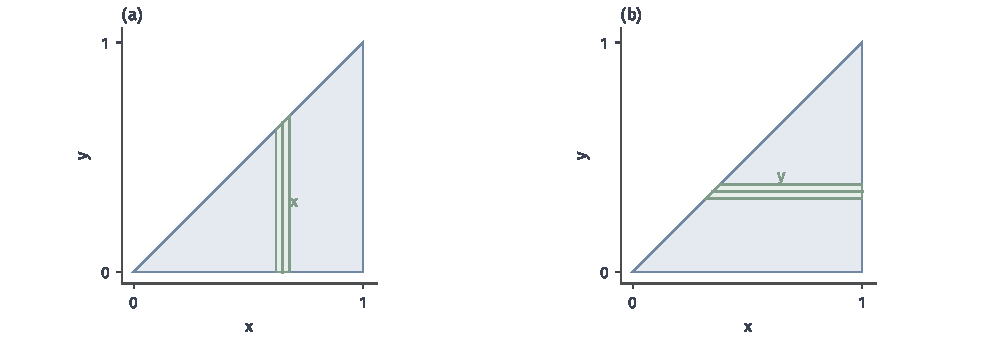
\includegraphics[width=169.0mm]{figures/01-mathematical-preliminaries-upper/00-shared/matplotlib/chapter3-concept-processes/region-slicing-orders.pdf}
 \caption{$D=\{0\leq y\leq x\leq1\}$在两图完全相同。(a) 固定$x$，纵截面为$0\leq y\leq x$；(b) 固定$y$，横截面为$y\leq x\leq1$。绿色窄条仅示意一次切片，图中的条宽不充当实际微元。两种累计$1$都得面积$1/2$；换序依据非负性或绝对可积性，而非图形本身。}
 \label{fig:analysis-process-region-slicing-orders}
\end{figure*}

换序有时决定一个积分能否算出来。
\begin{example}[换序计算含$e^{y^2}$的累次积分]
\label{ex:region-exp-square-order-swap}
考虑
\[
 \int_0^1\left(\int_x^1e^{y^2}\,\mathrm dy\right)\mathrm dx.
\]
内层的$e^{y^2}$没有初等原函数，按原次序无法用原函数直接计算。
积分区域是闭三角形$\{(x,y):0\leq x\leq y\leq1\}$，被积函数在其上连续，因而绝对可积，可以交换次序。
固定$y\in[0,1]$时，横截面是$0\leq x\leq y$，于是
\[
 \int_0^1\left(\int_0^ye^{y^2}\,\mathrm dx\right)\mathrm dy
 =\int_0^1ye^{y^2}\,\mathrm dy
 =\frac{e-1}{2}.
\]
\end{example}

内层对$x$积分时$e^{y^2}$是常数，只产生截面长度$y$，而这个因子$y$恰好使外层积分有原函数$\frac12e^{y^2}$。

\subsubsection{积分换序的适用边界}

非负函数没有正负相消，累计可以为无穷；绝对可积函数允许取正负值，但正负两部分的累计各自有限。
两者都缺失时，两种累计次序可能以不同方式配对正负贡献，交换次序就可能改变结果，甚至一个次序收敛而另一个次序发散。

最直观的例子来自双重级数。
设$a_{i,j}$（$i,j\geq1$）是一个无穷矩阵，在第一象限上令
$f(x,y)=a_{i,j}$于$(x,y)\in[i-1,i)\times[j-1,j)$，即每个边长为$1$的方格上取对应的矩阵元素。
对$x\in[i-1,i)$，截面积分$\int_0^\infty f(x,y)\,\mathrm dy=\sum_ja_{i,j}$是第$i$行的和（在各项非负或该行绝对收敛时）；再对$x$积分，就得到“先行后列”的累次和$\sum_i\sum_ja_{i,j}$。
另一种次序同理给出$\sum_j\sum_ia_{i,j}$，而$\int|f|\,\mathrm dm_2=\sum_{i,j}|a_{i,j}|$。

因此，Tonelli定理说明非负双重级数可以任意交换求和次序，Fubini定理说明绝对收敛的双重级数也可以这样做。
缺少绝对收敛时，即使每一行、每一列的和都有限，两种次序也可能给出不同的结果。

\begin{example}[行列各自可加仍不足以换序]
\label{ex:analysis-iterated-sum-failure}
令$a_{i,j}=\mathbb I\{j=i\}-\mathbb I\{j=i+1\}$（$i,j\geq1$），并按上面的方格构造第一象限上的阶梯函数$f$。
每一行只有一个$1$和一个$-1$，故$\sum_j a_{i,j}=0$；
第一列只有$a_{1,1}=1$，和为$1$；第$j\geq2$列有$a_{j,j}=1$与$a_{j-1,j}=-1$，和为$0$。于是
\[
 \sum_{i=1}^{\infty}\left(\sum_{j=1}^{\infty}a_{i,j}\right)=0,
 \qquad
 \sum_{j=1}^{\infty}\left(\sum_{i=1}^{\infty}a_{i,j}\right)=1,
\]
即$f$的两种累次积分分别为$0$和$1$。
两种累次积分都有有限值，却不相等。每行的绝对值和为$2$，所以$\int|f|\,\mathrm dm_2=+\infty$，
正负部分也各为无穷。失效的是Fubini定理的绝对可积条件，而非某一行的计算规则。
\end{example}

图~\ref{fig:vol1-add-fubini-cancellation-grid}显示这个例子的两条对角线。
逐行求和时，每个$+1$与同一行右侧的$-1$配对；逐列求和时，每个$-1$与同一列下方的$+1$配对，第一列的$+1$则没有配对对象。
由于绝对和无穷，Fubini定理不能保证这两种配对给出同一结果。
\begin{figure}[!htb]
  \centering
  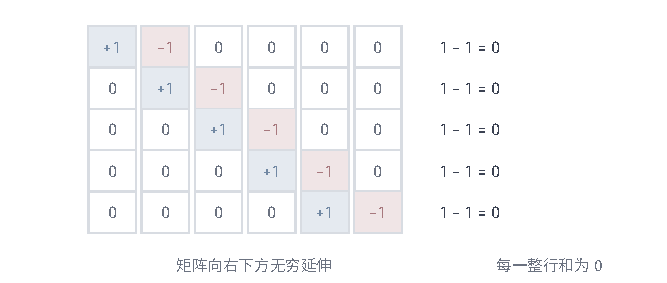
\includegraphics[width=112mm]{figures/01-mathematical-preliminaries-upper/00-shared/tikz/mathematical-language-combinatorics-analysis-optimization-comprehension-additions/fubini-cancellation-grid.pdf}
  \caption{无穷矩阵$a_{i,j}=\mathbb I\{j=i\}-\mathbb I\{j=i+1\}$的左上角，展示前五行、前六列，矩阵向右下方继续；每个单元格也可看成第一象限中边长为$1$的方格。每一整行的和为$0$；第一整列的和为$1$，其他整列的和为$0$。蓝、红单元分别为$+1,-1$，每行绝对和为$2$，因而无穷矩阵不绝对可加。}
  \label{fig:vol1-add-fubini-cancellation-grid}
\end{figure}

连续函数也会出现同样的现象。
\begin{example}[$(x^2-y^2)/(x^2+y^2)^2$的两种累次积分不同]
\label{ex:region-rational-non-fubini}
在$(0,1)^2$上取
\[
 f(x,y)=\frac{x^2-y^2}{(x^2+y^2)^2}.
\]
直接求导可得$\partial_y\bigl(y/(x^2+y^2)\bigr)=f(x,y)$，所以固定$x>0$时
\[
 \int_0^1f(x,y)\,\mathrm dy=\left[\frac{y}{x^2+y^2}\right]_{y=0}^{y=1}=\frac{1}{1+x^2},
\]
再对$x$积分得到$\pi/4$。
由于$f(y,x)=-f(x,y)$，先对$x$积分时内层结果是$-1/(1+y^2)$，这一次序得到$-\pi/4$。

两个结果不同，原因仍是绝对可积性失效。
在$0<y<x$处$f>0$，所以
\[
 \int_0^1|f(x,y)|\,\mathrm dy\geq\int_0^xf(x,y)\,\mathrm dy=\left[\frac{y}{x^2+y^2}\right]_{y=0}^{y=x}=\frac{1}{2x},
\]
而$\int_0^11/(2x)\,\mathrm dx=+\infty$，由Tonelli定理，$\int_{(0,1)^2}|f|\,\mathrm dm_2=+\infty$。
\end{example}

在极坐标下$|f|=|\cos2\theta|/r^2$，这正是示例~\ref{ex:region-power-function-threshold}中$p=2$的临界幂次：原点附近正负两部分各自累计无穷。

\subsection{区域积分的换元}
\label{sec:multivariable-change-variables}

累次积分保留原坐标，只改变累计次序。
换元则用一个向量值映射$T$改变位置的坐标表示，例如用半径与角度描述圆盘中的点。
换坐标以后，函数要按新坐标重写，每个小块的体积也要重新计算：参数空间中大小相同的小块，映到原空间后可能大小不同。

\subsubsection{换元公式与适用条件}

\paragraph{体积的局部缩放}

一元换元$x=T(t)$中，参数的小区间$[t,t+\Delta t]$被映成长约$|T'(t)|\Delta t$的小区间，因子$|T'(t)|$记录长度的缩放（定理~\ref{thm:analysis-lebesgue-change-variables}）。
多元换元要把参数空间中的小块换成体积，先看线性映射。
方阵$\bm A$把单位正方体映成由$\bm A$的各列张成的平行多面体，其体积为$|\det\bm A|$；更一般地，对任意可测集合$E$都有$m_d(\bm AE)=|\det\bm A|\,m_d(E)$\scite{math-folland1999real}。

几个特例可以直接核对。
对角矩阵$\operatorname{diag}(a_1,\ldots,a_d)$分别伸缩各坐标，体积比例为$\prod_j|a_j|$，这正是坐标盒的体积规则。
正交矩阵（旋转与反射）保持距离，不改变图形的形状和大小，行列式为$\pm1$。
剪切矩阵$\begin{bmatrix}1&s\\0&1\end{bmatrix}$把正方形推成等底等高的平行四边形，面积不变，行列式也等于$1$。
公式取行列式的绝对值，是因为反射这类改变定向的映射行列式为负，而体积必须非负。

对可微的非线性映射$T$，由式~\eqref{eq:analysis-jacobian-linearization}，在一点$\bm x$附近有$T(\bm x+\bm h)\approx T(\bm x)+\bm J_T(\bm x)\bm h$。
于是以$\bm x$为角、边长为$\varepsilon$的小方块$Q$，被$T$映成一个近似的平行多面体，其体积约为$|\det\bm J_T(\bm x)|\varepsilon^d$；图~\ref{fig:analysis-process-jacobian-grid-cell}画出了这种小块的变化。

设$g$是原空间中的密度。用小方块$Q_k$铺满参数区域，记$\bm x_k$为$Q_k$的一个角，每块映成的小块$T(Q_k)$中的质量约为
\[
 g(T(\bm x_k))\,m_d(T(Q_k))\approx g(T(\bm x_k))|\det\bm J_T(\bm x_k)|\varepsilon^d.
\]
对$k$求和后，左侧的和近似原空间中的总质量，右侧的和近似参数空间中函数$g(T(\bm x))|\det\bm J_T(\bm x)|$的积分。
因此$g\circ T\,|\det\bm J_T|$是“每单位参数体积所含的质量”：它把原空间中按单位体积计的密度，换算成按参数小块计的密度。

这个局部说明还不是整个积分公式的证明。
整体上还必须控制每块的近似误差在加总以后趋于零，并且确保$T$把每个点只覆盖一次：若两个参数小块映到同一块正体积区域，那里的质量就会被计算两次。

\paragraph{勒贝格积分的换元}

开集之间的$C^1$微分同胚同时满足这两项要求：连续可微保证局部的体积规则，双射保证全局只覆盖一次。
定理直接对勒贝格可测函数陈述，连续被积函数是其特例。
\begin{theorem}[区域积分的换元公式]
设$U,V\subseteq\mathbb R^d$为开集，$T:U\to V$为$C^1$双射，逆映射也为$C^1$，且$\det\bm J_T$处处非零。
对任意非负勒贝格可测函数$g:V\to[0,\infty]$，有
\begin{equation}
 \int_Vg(\bm y)\,\mathrm d\bm y
 =\int_Ug(T(\bm x))|\det\bm J_T(\bm x)|\,\mathrm d\bm x,
 \label{eq:measurable-change-variables}
\end{equation}
允许共同值为$+\infty$。若$g$有符号且在$V$上绝对可积，则变换后的函数也绝对可积，等式仍成立并取有限值。
\end{theorem}

这类变换及其逆在定义域的每个闭有界子集上满足Lipschitz条件，因而把零测集映为零测集。
所以勒贝格可测函数$g$与$T$复合后仍勒贝格可测：Borel集合的原像仍是Borel集合，零测集的原像仍是零测集，而每个勒贝格可测集都是Borel集合与零测集子集之并。

一般定理先建立可测集合的体积变换$m_d(T(E))=\int_E|\det\bm J_T|$，再从指示函数进入简单函数，最后以单调逼近得到非负函数的公式；有符号情形对$|g|$、$g^+$和$g^-$分别应用非负结论即可。
这里说明的是证明的依赖关系，集合层的体积变换定理引用测度论教材\scite{math-folland1999real}，不把逐点线性化当作完整证明。

若只在可测子区域$D\subseteq U$上积分，对$V$中的函数$g\mathbb I_{T(D)}$应用同一公式，即得
\begin{equation}
 \int_{T(D)}g(\bm y)\,\mathrm d\bm y
 =\int_Dg(T(\bm x))|\det\bm J_T(\bm x)|\,\mathrm d\bm x.
 \label{eq:analysis-multivariate-change-variables}
\end{equation}
这里不另加有界或边界零测的要求；所需条件仍是非负可测，或者有符号且绝对可积。

常用坐标在原点、坐标轴或角度的接缝处不是微分同胚，例如极坐标在原点处所有角度都对应同一点。
若在参数区域和原区域中各去掉一个零测集以后，参数化成为开集之间的$C^1$微分同胚，就可以先在剩下的范围内换元，再补回零测集，因为零测集对积分没有贡献。
若参数化在正测度区域上重复覆盖，则不能直接使用这个单次覆盖版本。

\subsubsection{常用坐标变换}

\paragraph{极坐标}

圆盘的边界用直角坐标描述时，积分上下限会含平方根。
以半径$r$和角度$\theta$作为坐标，圆盘变成参数矩形$[0,1]\times[0,2\pi]$，但面积权重必须增加半径因子。
在平面上画出同心圆$r=$常数与射线$\theta=$常数组成的网格：介于$r$与$r+\Delta r$、$\theta$与$\theta+\Delta\theta$之间的小块，径向边长为$\Delta r$，弧向边长约为$r\Delta\theta$，所以面积约为$r\Delta r\Delta\theta$。
同样大小的参数块，离原点越远，对应的面积越大；靠近原点时则被压缩得很小。
这一面积权重正是极坐标映射的Jacobian行列式：示例~\ref{ex:multivariable-polar-jacobian}已算出$\det\bm J=r$。下面用它计算单位圆盘的面积，并检查换元公式的条件。
\begin{example}[用极坐标计算单位圆盘的面积]
\label{ex:analysis-polar-coordinate-jacobian}
令$D=\{\bm x\in\mathbb R^2:\lVert\bm x\rVert_2\leq1\}$，并令$T(r,\theta)=(r\cos\theta,r\sin\theta)$。
在开集$U=(0,1)\times(0,2\pi)$上，$T$是到$V$的$C^1$双射，逆映射也是$C^1$，其中$V$是开圆盘去掉线段$[0,1)\times\{0\}$（含原点）后的区域。
由示例~\ref{ex:multivariable-polar-jacobian}，$|\det\bm J_T(r,\theta)|=r$，在$U$上处处非零。
$D$与$V$只相差边界圆周和线段$[0,1)\times\{0\}$，它们都是零测集，因此
\[
 \int_D1\,\mathrm d\bm x
 =\int_V1\,\mathrm d\bm x
 =\int_0^{2\pi}\int_0^1r\,\mathrm dr\,\mathrm d\theta
 =\pi.
\]
最后一步在参数矩形上使用Tonelli定理，积分上下限包含端点不改变积分值。
若让$\theta$取遍$(0,4\pi)$，圆盘就会被覆盖两次，按公式算出的$2\pi$不再是面积，这正是单次覆盖条件排除的情形。
\end{example}

图~\ref{fig:vol1-add-polar-area-weight}说明半径因子来自哪里。同样的角度变化在较大半径处扫过更长的弧，故同样大小的参数块对应更大的面积，积分权重必须随半径变化。
\begin{figure}[!htb]
  \centering
  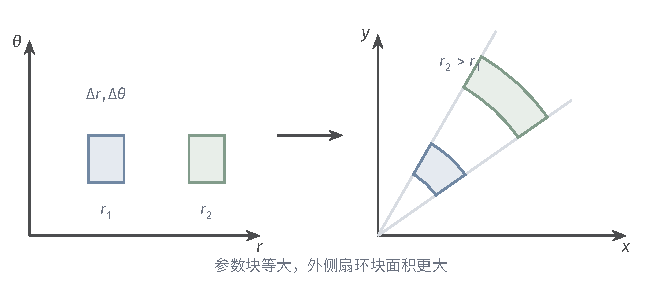
\includegraphics[width=112mm]{figures/01-mathematical-preliminaries-upper/00-shared/tikz/mathematical-language-combinatorics-analysis-optimization-comprehension-additions/polar-area-weight.pdf}
  \caption{极坐标映射中的两个等大参数块，具有相同的$\Delta r,\Delta\theta$，但外侧半径$r_2$较大。对应扇环块的精确面积为$(r\Delta r+(\Delta r)^2/2)\Delta\theta$，一阶项为$r\Delta r\Delta\theta$，因此面积元为$r\,\mathrm dr\,\mathrm d\theta$。图只比较局部块，坐标原点与接缝的处理见正文。}
  \label{fig:vol1-add-polar-area-weight}
\end{figure}

用极坐标可以直接核对示例~\ref{ex:region-power-function-threshold}得到的阈值。
\begin{example}[用极坐标核对幂函数的可积阈值]
\label{ex:region-polar-power-check}
设$0<a<b$，在圆环$\{a\leq\lVert\bm x\rVert_2\leq b\}$上积分$\lVert\bm x\rVert_2^{-p}$。
在开集$(a,b)\times(0,2\pi)$上使用极坐标，被去掉的两条圆周和一条线段都是零测集；被积函数只依赖半径，于是
\[
 \int_{a\leq\lVert\bm x\rVert_2\leq b}\lVert\bm x\rVert_2^{-p}\,\mathrm d\bm x
 =\int_0^{2\pi}\int_a^br^{-p}\cdot r\,\mathrm dr\,\mathrm d\theta
 =2\pi\int_a^br^{1-p}\,\mathrm dr.
\]
令$a\downarrow0$，它有界当且仅当$1-p>-1$，即$p<2$；令$b\to\infty$，它有界当且仅当$1-p<-1$，即$p>2$，与壳层估计一致。
取$p=0$、$a=1$、$b=2$，得到$2\pi\int_1^2r\,\mathrm dr=3\pi$，这就是示例~\ref{ex:region-power-function-threshold}中的$\alpha=m_2(A_0)$。
\end{example}

面积因子$r$正是壳层估计中“面积随半径增长”的来源：半径约为$r$、厚度为$\Delta r$的细圆环，面积约为$2\pi r\Delta r$。

极坐标与累次积分结合，还能计算一个没有初等原函数的一元积分。
\begin{example}[用极坐标计算Gauss积分]
\label{ex:region-gauss-integral}
函数$e^{-x^2}$没有初等原函数，但平面函数$e^{-(x^2+y^2)}$非负，在极坐标下只依赖半径。
对开集$(0,\infty)\times(0,2\pi)$使用换元公式，被去掉的原点和正$x$轴是零测集，于是
\[
 \int_{\mathbb R^2}e^{-(x^2+y^2)}\,\mathrm d(x,y)
 =\int_0^{2\pi}\int_0^\infty e^{-r^2}r\,\mathrm dr\,\mathrm d\theta
 =2\pi\cdot\frac12=\pi.
\]
另一方面，由Tonelli定理，左侧等于
\[
 \begin{aligned}
 \int_{\mathbb R}\left(\int_{\mathbb R}e^{-x^2}e^{-y^2}\,\mathrm dy\right)\mathrm dx
 &=\int_{\mathbb R}e^{-x^2}\,\mathrm dx\cdot\int_{\mathbb R}e^{-y^2}\,\mathrm dy\\
 &=\left(\int_{\mathbb R}e^{-x^2}\,\mathrm dx\right)^2.
 \end{aligned}
\]
这个积分为正，因此$\int_{\mathbb R}e^{-x^2}\,\mathrm dx=\sqrt\pi$。
\end{example}

这个结果给出正态分布密度的归一化常数。
计算同时用到了换元和累次积分：换元把平面积分变成可算的径向积分，累次积分把同一个平面积分拆成两个相同的一元积分。

\paragraph{柱坐标}

在三维中，柱坐标在极坐标之外保留高度$z$：
\[
 (x,y,z)=(r\cos\theta,r\sin\theta,z).
\]
参数小块对应的是一块极坐标小块再沿竖直方向拉高$\Delta z$，体积约为$r\Delta r\Delta\theta\Delta z$。
Jacobian矩阵左上角是极坐标的$2\times2$块，右下角为$1$，其余元素为零，行列式仍为$r$，故体积元是$r\,\mathrm dr\,\mathrm d\theta\,\mathrm dz$。
用这个体积元可以直接算出圆柱体的体积。
\begin{example}[圆柱体的体积]
\label{ex:region-cylinder-volume}
半径$R$、高度$H$的圆柱体由$0\leq r\leq R$、$0\leq\theta\leq2\pi$、$0\leq z\leq H$描述。
与极坐标相同，在开参数长方体$(0,R)\times(0,2\pi)\times(0,H)$上换元，去掉的竖直半平面片和圆柱表面都是零测集。于是
\[
 \int_0^H\int_0^{2\pi}\int_0^R r\,\mathrm dr\,\mathrm d\theta\,\mathrm dz
 =H\cdot2\pi\cdot\frac{R^2}{2}=\pi R^2H.
\]
\end{example}

关于竖直轴对称的物体，如圆柱、圆锥、旋转抛物面所围的区域，用柱坐标描述时上下限最简单。

\paragraph{球坐标}

球坐标用到原点的距离$\rho$、从正$z$轴量起的夹角$\varphi$和绕$z$轴的角$\theta$：
\[
 (x,y,z)=(\rho\sin\varphi\cos\theta,\rho\sin\varphi\sin\theta,\rho\cos\varphi).
\]
在球面上，$\varphi$相当于纬度（从北极量起），$\theta$相当于经度。
参数小块对应的近似长方体有三条边：沿径向长$\Delta\rho$；沿经线长$\rho\Delta\varphi$；沿纬线圆长$\rho\sin\varphi\Delta\theta$，因为纬线圆的半径是$\rho\sin\varphi$。
三边相乘得到体积约为$\rho^2\sin\varphi\,\Delta\rho\Delta\varphi\Delta\theta$；靠近两极时纬线圆变小，参数小块对应的体积也随之变小。

按$(\rho,\varphi,\theta)$的次序写出Jacobian矩阵，沿第三行展开行列式，
\[
 \det\begin{bmatrix}
 \sin\varphi\cos\theta&\rho\cos\varphi\cos\theta&-\rho\sin\varphi\sin\theta\\
 \sin\varphi\sin\theta&\rho\cos\varphi\sin\theta&\rho\sin\varphi\cos\theta\\
 \cos\varphi&-\rho\sin\varphi&0
 \end{bmatrix}
\]
等于
\[
 \cos\varphi\cdot\rho^2\sin\varphi\cos\varphi+\rho\sin\varphi\cdot\rho\sin^2\varphi
 =\rho^2\sin\varphi,
\]
与几何估计一致；在$0<\varphi<\pi$上它为正，故体积元为$\rho^2\sin\varphi\,\mathrm d\rho\,\mathrm d\varphi\,\mathrm d\theta$。
用这个体积元可以算出球的体积。
\begin{example}[球的体积]
\label{ex:region-ball-volume}
半径$R$的球由$0\leq\rho\leq R$、$0\leq\varphi\leq\pi$、$0\leq\theta\leq2\pi$描述。
和极坐标一样，在开参数长方体$(0,R)\times(0,\pi)\times(0,2\pi)$上换元，它覆盖的是球内部去掉半平面片$\{y=0,\ x\geq0\}$后的区域；被去掉的半平面片（其中包含$z$轴上的一段）与球面都是零测集，补回后不改变积分。于是
\[
 \int_0^{2\pi}\int_0^\pi\int_0^R\rho^2\sin\varphi\,\mathrm d\rho\,\mathrm d\varphi\,\mathrm d\theta
 =2\pi\cdot2\cdot\frac{R^3}{3}
 =\frac{4\pi R^3}{3},
\]
其中$\int_0^\pi\sin\varphi\,\mathrm d\varphi=2$，$\int_0^R\rho^2\,\mathrm d\rho=R^3/3$。
\end{example}

球在球坐标下变成参数长方体，三组上下限都是常数；以原点为中心对称的区域，或只依赖$\rho$的被积函数，用球坐标计算最简单。

\subsection{参数积分}
\label{sec:multivariable-parameter-integrals}

换元改变的是空间坐标。
参数积分则固定积分区域，让被积函数依赖一个实参数$\theta$，研究积分所得的总量怎样随参数变化。
例如$\theta$是时间，$g(\bm x,\theta)$是时刻$\theta$的质量密度，积分就是该时刻的总质量；或者$\theta$是模型中的参数，积分是依赖该参数的平均损失。
这里要回答三个问题：总量是否随参数连续变化，总量的变化率能否由密度的变化率累计得到，以及积分区间的端点也随参数移动时怎样求导。

\subsubsection{参数积分的定义}

设$D\in\mathcal L(\mathbb R^d)$，$I$为实参数区间，且对每个$\theta\in I$，$g(\cdot,\theta)$都是$D$上可积的标量函数。定义
\[
 G(\theta)=\int_Dg(\bm x,\theta)\,\mathrm d\bm x.
\]
固定参数后，$\bm x$是被积变量；积分完成以后，$G$是参数$\theta$的一元函数。
例如$D=[0,\infty)$、$g(x,\theta)=e^{-\theta x}$（$\theta>0$）时，$G(\theta)=1/\theta$。

点态连续或点态可微只描述每个固定位置$\bm x$处的变化。
总量$G$还可能因为“质量”在参数变化时移向无穷远，或集中到越来越小的区域而突变，这些现象在任何固定位置都看不出来。
下面的例子中，密度在每一点都趋于零，总质量却保持不变。
\begin{example}[$\theta e^{-\theta x}$的质量逃向无穷远]
\label{ex:region-escaping-mass}
在$[0,\infty)$上令$g(x,\theta)=\theta e^{-\theta x}$（$\theta>0$）。对每个$\theta>0$，
\[
 G(\theta)=\int_0^\infty\theta e^{-\theta x}\,\mathrm dx=1.
\]
另一方面，$\theta\downarrow0$时，对每个固定的$x$都有$g(x,\theta)\to0$。
质量被摊薄并推向远处：由$\int_c^\infty\theta e^{-\theta x}\,\mathrm dx=e^{-\theta c}$，总质量的一半位于$x\geq(\log2)/\theta$的位置，而这个位置随$\theta\downarrow0$趋于无穷远。
若在$\theta=0$处按点态极限令$g(x,0)=0$，则$G(0)=0\neq1=\lim_{\theta\downarrow0}G(\theta)$。
\end{example}

可见点态极限本身不能决定总量的极限；要把点态性质传递给$G$，还需要控制整族函数，防止质量逃逸。

\subsubsection{参数积分的连续性}

所需的控制由支配收敛定理提供：用同一个可积函数控制附近全部参数的密度，贡献就不能集中到越来越小的区域，也不能移向无穷远。
\begin{theorem}[可积控制下参数积分的连续性]
设$\theta_0\in I$，每个$g(\cdot,\theta)$可测。假设存在$\theta_0$在$I$中的一个相对邻域$J$、同一个可测零测集$N$及非负可积函数$h$，使对每个$\bm x\in D\setminus N$，$g(\bm x,\cdot)$在$\theta_0$连续，且
$|g(\bm x,\theta)|\leq h(\bm x)$对所有$\theta\in J$成立。
则$G(\theta)$在$J$上有有限值，并在$\theta_0$连续。
\end{theorem}
\begin{proof}
任取$\theta_n\to\theta_0$，充分大时$\theta_n\in J$。在$D\setminus N$上，$g(\bm x,\theta_n)\to g(\bm x,\theta_0)$，且绝对值都不超过$h(\bm x)$。
支配收敛给出$G(\theta_n)\to G(\theta_0)$，由序列判据得到连续性。
\end{proof}

控制函数$h$的作用是给所有邻近参数的密度一个共同的、总量有限的上方包络，质量就无法逃到包络以外。
示例~\ref{ex:region-escaping-mass}中不存在这样的包络：对任意$\delta>0$，当$x>1/\delta$时，
\[
 \sup_{0<\theta<\delta}\theta e^{-\theta x}=\frac{1}{ex},
\]
上确界在$\theta=1/x$处取到，而$1/(ex)$在$(1/\delta,\infty)$上不可积。

相反，对$g(x,\theta)=e^{-\theta x}$，固定$\theta_0>0$，在邻域$\theta>\theta_0/2$内有$e^{-\theta x}\leq e^{-\theta_0x/2}$，后者在$[0,\infty)$上可积，故$G$在$\theta_0$连续。
控制函数只需覆盖所考察参数点的邻域，不要求同一上界适用于全部参数；这里每个$\theta_0>0$各用一个包络，就得到$G$在整个$(0,\infty)$上连续。

\subsubsection{积分号下求导}

若$g(\bm x,\theta)$是时刻$\theta$的密度，自然希望总质量的变化率等于各处密度变化率的累计，即$G'(\theta)=\int_D\partial_\theta g(\bm x,\theta)\,\mathrm d\bm x$。
这实际是交换参数差商的极限与积分。
各点偏导数存在只确定差商的点态极限；用同一个可积函数控制全部差商，才足以将这个极限移入积分号。
\begin{theorem}[可积导数界下的积分号内求导]
设$I$是包含$\theta_0$的开区间，对每个$\theta\in I$，$\bm x\mapsto g(\bm x,\theta)$可测，并且$g(\cdot,\theta_0)$可积。
假设存在一个可测零测集$N$，使每个$\bm x\in D\setminus N$处的$\theta\mapsto g(\bm x,\theta)$在整个$I$内可微；对每个$\theta$，偏导数作为$\bm x$的函数可测，并且存在非负可积函数$h$使
\begin{equation}
 \left|\frac{\partial g}{\partial\theta}(\bm x,\theta)\right|\leq h(\bm x)
 \quad\text{对所有$\bm x\in D\setminus N$及所有$\theta\in I$成立},
 \label{eq:analysis-parameter-derivative-domination}
\end{equation}
则对每个$\theta\in I$，$g(\cdot,\theta)$在$D$上可积，且
\begin{equation}
 G'(\theta_0)=\int_D\frac{\partial g}{\partial\theta}(\bm x,\theta_0)\,\mathrm d\bm x.
 \label{eq:analysis-differentiate-under-integral}
\end{equation}
\end{theorem}
\begin{proof}
对$\bm x\notin N$，一元中值定理给出
$|g(\bm x,\theta)-g(\bm x,\theta_0)|\leq|\theta-\theta_0|h(\bm x)$，
所以$I$中每个$g(\cdot,\theta)$都被可积函数$|g(\cdot,\theta_0)|+|\theta-\theta_0|h$控制，因而可积，$G$在$I$内有有限值。
对非零$t$且$\theta_0+t\in I$，令
\[
 q_t(\bm x)=\frac{g(\bm x,\theta_0+t)-g(\bm x,\theta_0)}{t}.
\]
中值定理又给出
\[
 |q_t(\bm x)|\leq h(\bm x)\qquad(\bm x\notin N),
\]
并且$t\to0$时，$q_t(\bm x)$在$D\setminus N$上趋于$\partial g/\partial\theta(\bm x,\theta_0)$。
对任意非零序列$t_n\to0$应用支配收敛，都得到同一个积分极限$\int_D\partial_\theta g(\bm x,\theta_0)\,\mathrm d\bm x$；
由实数极限的序列判据，它就是差商$\bigl(G(\theta_0+t)-G(\theta_0)\bigr)/t$在$t\to0$时的极限，即式~\eqref{eq:analysis-differentiate-under-integral}。
\end{proof}

这里的零测集$N$和控制函数$h$都不能随参数改变：参数范围不可数，不能靠取全部参数例外集的并自动获得一个零测集。
条件~\eqref{eq:analysis-parameter-derivative-domination}是一组便于核对的充分条件；更一般的版本也可以直接控制参数差商。

控制函数通常只在所考察参数点的一个邻域内取得。
\begin{example}[对$e^{-\theta x}$在积分号下求导]
\label{ex:region-differentiate-exponential}
令$g(x,\theta)=e^{-\theta x}$，$x\in[0,\infty)$、$\theta>0$，则$G(\theta)=1/\theta$。
固定$\theta_0>0$，取$I=(\theta_0/2,3\theta_0/2)$，则对$\theta\in I$，
\[
 |\partial_\theta g(x,\theta)|=xe^{-\theta x}\leq xe^{-\theta_0x/2}=:h(x).
\]
分部积分给出$\int_0^\infty h(x)\,\mathrm dx=4/\theta_0^2<\infty$；不等式对每个$x$都成立，可取$N=\varnothing$。
由积分号下求导的定理，
\[
 G'(\theta_0)=-\int_0^\infty xe^{-\theta_0x}\,\mathrm dx=-\frac{1}{\theta_0^2},
\]
与$G(\theta)=1/\theta$的直接求导一致。
\end{example}

例中的控制函数依赖于$\theta_0$：若参数范围包含任意接近零的正数，$xe^{-\theta_0x/2}$就不再控制全部导数。
交换求导与积分所需的，只是所考察参数点附近的统一控制。

若所考察参数点附近找不到可积的导数界，交换求导与积分可能失败。
下面的反例发生在参数区间的端点$\theta=0$，考察的是右导数。
\begin{example}[参数积分中的控制函数失效]
\label{ex:analysis-parameter-integral-failure}
对$\theta\geq0$与$x\in(0,1)$，定义
\[
 g(x,\theta)=
 \begin{cases}
 \dfrac{\theta x}{x^2+\theta^2}, & \theta>0,\\[5pt]
 0, & \theta=0.
 \end{cases}
\]
在$\theta=0$处，对每个固定$x>0$，差商$g(x,\theta)/\theta=x/(x^2+\theta^2)\to1/x$，所以关于$\theta$的右偏导数都等于$1/x$，但$1/x$在$(0,1)$上不可积。
直接积分（令$u=x^2+\theta^2$）得到
\[
 G(\theta)=\frac{\theta}{2}\log\left(\frac{1+\theta^2}{\theta^2}\right)\quad(\theta>0),
 \qquad G(0)=0.
\]
于是$G(\theta)/\theta=\frac12\log(1+\theta^{-2})$在$\theta\downarrow0$时发散，$G$在$0$处没有有限右导数。
积分内的逐点右导数虽然存在，却缺少统一可积控制，因此这里不能交换右求导与积分。
\end{example}

从密度的角度看，$g(\cdot,\theta)$在$x=\theta$处取峰值$1/2$；$\theta$变小时峰值向原点移动，差商$g(\cdot,\theta)/\theta$在峰值处等于$1/(2\theta)$，它的累计随之变得无界。

\subsubsection{变限积分的求导}

积分号下求导的定理固定了积分区域。
端点也变化时，即使被积函数不依赖参数，积分仍然会变化：例如$G(\theta)=\int_0^\theta1\,\mathrm dx=\theta$的导数为$1$，而被积函数对参数的偏导数为零，只累计偏导数会遗漏端点移动的贡献。

用质量来理解：区间$[a(\theta),b(\theta)]$上的总质量有两种变化来源，一是区间内部各处的密度在变，二是端点移动时把新的位置划入或划出区间。
右端点在参数增加$\Delta\theta$时向右移动约$b'(\theta)\Delta\theta$，新划入的一小段上密度约为$g(b(\theta),\theta)$，带来质量约$g(b(\theta),\theta)b'(\theta)\Delta\theta$；左端点向右移动则划出一小段，减少质量约$g(a(\theta),\theta)a'(\theta)\Delta\theta$。
要用端点处的函数值估计这一小段的质量，被积函数需要在端点附近连续。
\begin{theorem}[变限参数积分的求导]
设$a(\theta),b(\theta)$在$\theta_0$附近可微，且$a(\theta)<b(\theta)$。
若$g(x,\theta)$和$\partial_\theta g(x,\theta)$在包含这些邻近积分区间的一个紧矩形上连续，则
\begin{equation}
 \begin{aligned}
 \frac{\mathrm d}{\mathrm d\theta}\int_{a(\theta)}^{b(\theta)}g(x,\theta)\,\mathrm dx
 &=\int_{a(\theta)}^{b(\theta)}\partial_\theta g(x,\theta)\,\mathrm dx\\
 &\quad+g(b(\theta),\theta)b'(\theta)
 -g(a(\theta),\theta)a'(\theta).
 \end{aligned}
\label{eq:measurable-moving-boundary-integral}
\end{equation}
\end{theorem}
\begin{proof}
记$a_0=a(\theta_0)$、$b_0=b(\theta_0)$。积分差可分解为
\[
 \begin{aligned}
 G(\theta)-G(\theta_0)
 &=\int_{a_0}^{b_0}\bigl[g(x,\theta)-g(x,\theta_0)\bigr]\,\mathrm dx\\
 &\quad+\int_{b_0}^{b(\theta)}g(x,\theta)\,\mathrm dx
 -\int_{a_0}^{a(\theta)}g(x,\theta)\,\mathrm dx.
 \end{aligned}
\]
短区间积分按端点次序采用有向约定。
第一项是固定区间上的参数积分：$\partial_\theta g$在紧矩形上连续，因而有界，常数界在有界区间$[a_0,b_0]$上可积，满足条件~\eqref{eq:analysis-parameter-derivative-domination}，所以第一项除以$\theta-\theta_0$后趋于$\int_{a_0}^{b_0}\partial_\theta g(x,\theta_0)\,\mathrm dx$。
$g$在紧矩形上一致连续，当$\theta\to\theta_0$时，短区间$[b_0,b(\theta)]$上的$g(x,\theta)$一致地接近$g(b_0,\theta_0)$，所以第二项等于
$g(b_0,\theta_0)[b(\theta)-b_0]+o(|b(\theta)-b_0|)$。端点的可微性保证$|b(\theta)-b_0|=O(|\theta-\theta_0|)$，所以它的差商趋于$g(b_0,\theta_0)b'(\theta_0)$。
第三项同理，并保留前面的负号，得到下端点贡献。三项相加即得公式。
\end{proof}

紧矩形上的连续性是一组便于核对的充分条件。
对一般可测函数，公式中的端点值$g(b(\theta),\theta)$需要另外赋予意义：几乎处处相等的两个函数可以在端点上取不同的值，不能从几乎处处的等价类中直接读出边界上的值。

\FloatBarrier

\par\Needspace{10\baselineskip}
\section{路径积分}
\label{sec:multivariable-path-integration}

区域积分累计的是铺满一块区域的量，许多问题却只沿一条曲线累计。一根弯曲细铁丝的质量由各处的线密度和铁丝长度决定；把物体沿一条路线推过去，推力做的功不仅取决于力的大小和路线长度，还取决于力与前进方向的夹角。
两类问题都沿曲线累计，被积对象却不同：线密度在每一点只给出一个数，是标量函数；力在每一点给出一个带方向的量，是向量场。

相应地有两种路径积分。第一类路径积分把曲线切成小段，用每段上的函数值乘这段的实际长度再相加，铁丝质量就是这样算出的；它不关心沿哪个方向走过曲线。
第二类路径积分在每一小段上先取力与这段有向位移的内积，只保留力沿前进方向的分量，再把这些数相加；反向行走时每段位移都反号，积分也随之变号。

两种积分都要先用参数描述曲线，因此本节先说明路径与弧长，再分别讨论两类积分的定义、性质和计算。
最后研究力沿路径做的功什么时候只取决于起点和终点、而与中间的路线无关，这对应物理中保守力与势能的关系。
本节的参数积分都是一元勒贝格积分\scite{math-openstax-calculus3}。

\subsection{参数路径与弧长}
\label{sec:multivariable-line-integrals}

描述一次行进，需要知道每个时刻所在的位置。位置随时间连续变化，就得到一条路径；位置对时间的导数是速度，速度的大小称为速率。速率恒定时，速率乘经过的时间就是走过的路程。
本小节先给出路径的定义，再用折线逼近说明：速率随时间变化时，路程等于速率对时间的积分。

\subsubsection{路径的定义}

\paragraph{参数化路径}

不妨把参数$t$看成时间，把$\gamma(t)$看成一个质点在时刻$t$所在的位置。同一组位置可以走得快或慢，可以从任一端出发，也可以来回走好几遍；只记下经过了哪些点，就会丢失这些信息。用区间到空间的连续映射描述行进过程，位置和先后次序就一起保留了下来。
\begin{definition}[路径]
设$a<b$。连续映射$\gamma:[a,b]\to\mathbb R^d$称为一条\term{路径}（path），$\gamma(a)$和$\gamma(b)$分别为起点和终点；若两者相等，称为闭路径。
集合$C=\gamma([a,b])$称为路径的像。
\end{definition}

像集$C$只记录质点经过的位置，参数$t$还规定了经过的先后次序，所以同一个像集可以对应行进方式完全不同的路径。
\begin{example}[同一条对角线段上的三条路径]
\label{ex:analysis-diagonal-segment-paths}
以下三条平面路径的像都是连接$(0,0)$与$(1,1)$的对角线段：
\begin{itemize}
 \item $\gamma(t)=(t,t)^\top$，$0\leq t\leq1$，从$(0,0)$走到$(1,1)$，速度为$(1,1)^\top$；
 \item $\eta(u)=(u/2,u/2)^\top$，$0\leq u\leq2$，同样从$(0,0)$走到$(1,1)$，速度减半为$(1/2,1/2)^\top$，用时加倍；
 \item $\rho(t)=(t,t)^\top$（$0\leq t\leq1$）、$\rho(t)=(2-t,2-t)^\top$（$1\leq t\leq2$），先走到$(1,1)$再原路返回。
\end{itemize}
$\gamma$与$\eta$只是快慢不同，线段上每个点都恰好经过一次。$\rho$的像仍是这条线段，但每个内点被经过两次：去程一次，回程一次。
\end{example}

后面会看到，两种路径积分对$\gamma$与$\eta$都给出相同结果；沿$\rho$按长度累计时，结果是沿$\gamma$的两倍，按有向位移累计时，去程与回程恰好抵消。
可见路径积分是沿“一次行进”定义的，只知道像集还不能确定它。要计算一根铁丝的质量，应选一条把铁丝恰好走一遍的路径。

\paragraph{分段光滑路径}

示例~\ref{ex:analysis-diagonal-segment-paths}中的往返路径$\rho$在$t=1$处突然掉头，正方形边界在四个角处突然转向。这些位置没有唯一的切线方向，但在每一段直线上速度都存在且连续。为了把折线、多边形边界这类常见路径纳入计算，允许路径在有限个参数点处分段。
\begin{definition}[分段光滑路径]
若存在分割$a=t_0<t_1<\cdots<t_n=b$，使$\gamma$在每个$[t_{j-1},t_j]$上为$C^1$映射，称$\gamma$为分段$C^1$路径，也称分段光滑路径。
若每段内部还满足$\gamma'(t)\neq\bm0$，称该路径分段正则。
\end{definition}

这里“在闭区间$[t_{j-1},t_j]$上为$C^1$”是指该段内部的导数连续，并能连续延拓到该段的两个端点；相邻两段在公共端点处的导数不必相同。
例如$\rho$在$[0,1]$上的速度为$(1,1)^\top$，在$[1,2]$上的速度为$(-1,-1)^\top$。两段在$t=1$处的速度不同，但各自连续，所以$\rho$是分段$C^1$路径。

本节的路径积分都在分段$C^1$路径上定义。折点只有有限个，而参数区间中的有限点集测度为零，所以折点处的速度取什么值不影响参数积分。
分段正则要求每段内部速度不为零，排除了质点在某段中途停住的情形。本节的积分并不要求路径正则；后面用到单位切向量时，只在速度非零处使用它。

\subsubsection{路径的长度}

\paragraph{弧长}

测量一条弯曲道路的长度时，可以在路上依次插几根标杆，量出相邻标杆之间的直线距离再相加。每段直线距离都不超过对应那段路的实际长度，所以这样得到的折线长度不会超过道路长度；在两根标杆之间再插一根，由三角不等式，新折线的长度不会变短。标杆越密，折线越贴近道路，因此把实际长度定义为所有内接折线长度的上确界。
\begin{definition}[路径的弧长]
路径$\gamma:[a,b]\to\mathbb R^d$的弧长定义为
\[
 \ell(\gamma)=\sup_{a=t_0<\cdots<t_n=b}
 \sum_{j=1}^n\lVert\gamma(t_j)-\gamma(t_{j-1})\rVert_2.
\]
上确界取遍$[a,b]$的全部有限分割；若此值有限，称路径可求长。
\end{definition}

这个定义只用到路径上点的位置，不需要导数，所以任何连续路径都可以讨论它是否可求长。对分段光滑路径，弧长还可以用速度直接计算。在一小段参数区间$[t_{j-1},t_j]$上，质点的位移近似为速度乘时间：
$\gamma(t_j)-\gamma(t_{j-1})\approx\gamma'(t_{j-1})(t_j-t_{j-1})$，
所以这一小段的长度近似为速率$\lVert\gamma'(t_{j-1})\rVert_2$乘时间，汽车里程表正是这样累计路程的。把这些乘积相加并令分割变细，就得到下面的公式。
\begin{theorem}[分段光滑路径的弧长]
若$\gamma:[a,b]\to\mathbb R^d$分段$C^1$，则它可求长，且
\[
 \ell(\gamma)=\int_a^b\lVert\gamma'(t)\rVert_2\,\mathrm dt.
\]
\end{theorem}
\begin{proof}
加入分点不会使折线变短，所以计算上确界时只需考虑包含全部折点的分割；这样的折线长度按光滑段相加，弧长也按段相加。因此只需在一段$C^1$区间上证明，再把各段的等式相加。证明分两步：先说明任何折线都不比速度积分长，再说明足够细的折线与速度积分相差任意小。

第一步。对该段中的$\alpha<\beta$，由各坐标分量的一元基本定理，
$\gamma(\beta)-\gamma(\alpha)=\int_\alpha^\beta\gamma'(t)\,\mathrm dt$，这里向量的积分表示对各分量分别积分。
若弦$\gamma(\beta)-\gamma(\alpha)$非零，取它方向上的单位向量$\bm u$，则由Cauchy--Schwarz不等式
\[
 \lVert\gamma(\beta)-\gamma(\alpha)\rVert_2
 =\bm u^\top\bigl(\gamma(\beta)-\gamma(\alpha)\bigr)
 =\int_\alpha^\beta\bm u^\top\gamma'(t)\,\mathrm dt
 \leq\int_\alpha^\beta\lVert\gamma'(t)\rVert_2\,\mathrm dt;
\]
弦为零时这个不等式直接成立。同样的推理说明，任何连续向量值函数$\bm v$都满足$\lVert\int_\alpha^\beta\bm v\,\mathrm dt\rVert_2\leq\int_\alpha^\beta\lVert\bm v\rVert_2\,\mathrm dt$。
对任意分割把各段弦长相加，可知任意内接折线的长度都不超过$\int_a^b\lVert\gamma'\rVert_2\,\mathrm dt$，所以上确界也不超过它。

第二步。$\gamma'$在紧区间上一致连续。给定$\varepsilon>0$，取足够细的分割，使每个小区间上任意两点的$\gamma'$相距小于$\varepsilon$，并记$\Delta t_j=t_j-t_{j-1}$。
在第$j$个小区间上，
\[
 \gamma(t_j)-\gamma(t_{j-1})-\gamma'(t_{j-1})\Delta t_j
 =\int_{t_{j-1}}^{t_j}\bigl(\gamma'(t)-\gamma'(t_{j-1})\bigr)\,\mathrm dt,
\]
由第一步的范数不等式，它的范数不超过$\varepsilon\Delta t_j$；于是这一段的弦长与$\lVert\gamma'(t_{j-1})\rVert_2\Delta t_j$之差不超过$\varepsilon\Delta t_j$。
同一小区间上，$\int\lVert\gamma'\rVert_2\,\mathrm dt$与$\lVert\gamma'(t_{j-1})\rVert_2\Delta t_j$的差也不超过$\varepsilon\Delta t_j$。
两项相加后对$j$求和，速度积分与这条折线长度的差不超过$2\varepsilon(b-a)$，所以上确界不小于速度积分减$2\varepsilon(b-a)$。令$\varepsilon\downarrow0$，得到反向不等式。
\end{proof}

用这个公式可以计算示例~\ref{ex:analysis-diagonal-segment-paths}中三条路径的长度，并检验圆周长公式。
\begin{example}[对角线段与圆周的弧长]
对角线段$\gamma(t)=(t,t)^\top$，$0\leq t\leq1$，速度为$(1,1)^\top$，速率为$\sqrt2$，所以$\ell(\gamma)=\int_0^1\sqrt2\,\mathrm dt=\sqrt2$。两个坐标各变化$1$，走过的距离却不是$1+1=2$，而是斜边的长度。

慢速路径$\eta$的速率为$\sqrt2/2$，用时为$2$，长度为$\int_0^2(\sqrt2/2)\,\mathrm du=\sqrt2$。往返路径$\rho$在两段上的速率都是$\sqrt2$，总用时为$2$，长度为$2\sqrt2$。

半径为$r$的圆周可以参数化为$t\mapsto(r\cos t,r\sin t)^\top$，$0\leq t\leq2\pi$。速度为$(-r\sin t,r\cos t)^\top$，速率恒为$r$，长度为$\int_0^{2\pi}r\,\mathrm dt=2\pi r$，与圆周长公式一致。
\end{example}

$\gamma$与$\eta$的长度相同，因为速率减半恰好被用时加倍抵消；$\rho$的长度是$\gamma$的两倍，因为弧长把经过的次数也计算在内。

记$s(t)=\int_a^t\lVert\gamma'(u)\rVert_2\,\mathrm du$为截至时刻$t$累计走过的路程，它就是里程表在时刻$t$的读数。在每个光滑段内部，$s$对$t$的导数是速率$\lVert\gamma'(t)\rVert_2$，因此常把长度权重简写为
$\mathrm ds=\lVert\gamma'(t)\rVert_2\,\mathrm dt$，读作“一小段时间$\mathrm dt$内走过的一小段路程”。

\subsection{第一类路径积分}

第一类路径积分的被积对象是定义在曲线上的标量函数，例如铁丝各处的线密度或一条道路沿线各处的温度。每一小段的贡献是函数值乘这一小段的实际长度，因此它只需要路程这一个权重，不涉及方向。

\subsubsection{定义与可积性}

\paragraph{按弧长的积分}

设一根铁丝沿路径$\gamma$放置，$h(\bm x)$是它在点$\bm x$处的线密度，即单位长度的质量。线密度为常数时，质量等于密度乘长度；密度随位置变化时，把铁丝切成许多小段，每段上的密度近似为常数。
在参数小区间$[t_{j-1},t_j]$对应的一段上取一个时刻$\xi_j$，这段的质量约为
\[
 h(\gamma(\xi_j))\,\lVert\gamma'(\xi_j)\rVert_2\,(t_j-t_{j-1}),
\]
即“该处密度”乘“该段长度”。把各段相加，就得到参数区间上函数$h(\gamma(t))\lVert\gamma'(t)\rVert_2$的积分和，所以用这个函数的一元积分定义沿路径的累计。采用勒贝格积分，还能处理沿路径可测而不连续的标量函数。
\begin{definition}[第一类路径积分]
设$\gamma:[a,b]\to\mathbb R^d$分段$C^1$，$h:C\to\mathbb R$，其中$C=\gamma([a,b])$，且$h\circ\gamma$在参数区间上勒贝格可测。
若$h\geq0$，定义\term{第一类路径积分}（scalar line integral）为
\begin{equation}
 \int_\gamma h\,\mathrm ds
 =\int_a^b h(\gamma(t))\lVert\gamma'(t)\rVert_2\,\mathrm dt,
 \label{eq:analysis-scalar-line-integral}
\end{equation}
允许取$+\infty$。对一般有符号$h$，本节称它沿$\gamma$可积，是指
\[
 \int_a^b |h(\gamma(t))|\lVert\gamma'(t)\rVert_2\,\mathrm dt<\infty;
\]
此时由正负部分之差定义积分，式~\eqref{eq:analysis-scalar-line-integral}仍成立并取有限值。
\end{definition}

这个积分有几种常见读法。取$h=1$，积分就是弧长$\ell(\gamma)$；$h$是非负线密度时，积分是铁丝的总质量。

若$\ell(\gamma)>0$，比值
\[
 \bar h=\frac1{\ell(\gamma)}\int_\gamma h\,\mathrm ds
\]
是$h$沿曲线按长度的平均值：沿一条道路每隔相同路程记录一次温度再求平均，记录越密，结果越接近$\bar h$。
这里的平均按路程加权，而不按参数时间加权。若一辆车在某段路上开得很慢，按时间平均会让这段路的温度占更大比重，按路程平均则不受车速影响。

用一根密度不均匀的半圆铁丝可以说明质量和平均线密度的计算。
\begin{example}[上半圆铁丝的质量与平均线密度]
\label{ex:analysis-semicircle-wire}
沿上半单位圆$\gamma(t)=(\cos t,\sin t)^\top$，$0\leq t\leq\pi$，放一根铁丝，线密度为$h(x,y)=y$，即越高的地方越重。速度为$(-\sin t,\cos t)^\top$，速率恒为$1$，所以总质量为
\[
 \int_\gamma y\,\mathrm ds=\int_0^\pi\sin t\,\mathrm dt=2.
\]
铁丝长度为$\pi$，平均线密度为$\bar h=2/\pi\approx0.64$。两端$(\pm1,0)$处密度为零，顶点$(0,1)$处密度为$1$，平均值落在两者之间。
\end{example}
这条参数化的速率恒为$1$，参数时间与路程同步增长，所以按时间平均也得到$2/\pi$；速率不恒定时，两种平均一般不同。

若$h$在像集$C$上连续，由于$C$是紧区间在连续映射下的像，也是紧集，$h$在$C$上有界，绝对积分不超过$\sup_C|h|\,\ell(\gamma)<\infty$，因而$h$沿$\gamma$可积。连续性是方便的充分条件，并非定义本身的要求。

定义要求的是$h$在曲线上的实际取值，以及它与参数复合后的可测性。仅知道$h$作为平面函数勒贝格可积，并不能确定这个积分：平面上几乎处处相等的两个函数，沿同一条曲线的积分可以不同。
\begin{example}[平面积分为零而沿线段的积分为一]
令$h(x,y)=\mathbb I\{y=0\}$，它只在$x$轴上取$1$，在其余位置取$0$。$x$轴的平面测度为零，所以$h$与零函数在平面上几乎处处相等，$h$在平面上的积分为$0$。
沿$\gamma(t)=(t,0)^\top$，$0\leq t\leq1$，有$h(\gamma(t))=1$且速率为$1$，所以$\int_\gamma h\,\mathrm ds=1$；零函数沿同一路径的积分却是$0$。
\end{example}
原因是曲线本身的面积为零：改变平面函数在一个零面积集合上的值，不影响区域积分，却可能完全改变沿这个集合的路径积分。

\subsubsection{积分的基本性质}

下面各条性质中的有符号函数都假设沿所讨论的路径可积。把定义式~\eqref{eq:analysis-scalar-line-integral}代入一元勒贝格积分的相应性质，就逐项得到这些结论；用铁丝质量来读，每条性质都有直接的含义。

\paragraph{加法}

若$h,k$沿$\gamma$可积，则$h+k$也沿$\gamma$可积，且
\[
 \int_\gamma(h+k)\,\mathrm ds=\int_\gamma h\,\mathrm ds+\int_\gamma k\,\mathrm ds.
\]
绝对可积性由$|h+k|\leq|h|+|k|$保证，等式来自一元积分的加法。若铁丝由两种材料叠合而成，总质量等于两种材料各自的质量之和。

\paragraph{减法}

把$k$换成$-k$，它同样沿$\gamma$可积，由加法得到
\[
 \int_\gamma(h-k)\,\mathrm ds=\int_\gamma h\,\mathrm ds-\int_\gamma k\,\mathrm ds.
\]
两个积分都是有限数，所以相减时不会出现$\infty-\infty$。

\paragraph{数乘}

若$c\in\mathbb R$且$h$沿$\gamma$可积，则
\[
 \int_\gamma ch\,\mathrm ds=c\int_\gamma h\,\mathrm ds.
\]
把每一小段上的密度同时放大$c$倍，总质量也放大$c$倍。

\paragraph{路径拼接}

若$\gamma_1$的终点是$\gamma_2$的起点，记先走$\gamma_1$、再走$\gamma_2$的拼接路径为$\gamma_1*\gamma_2$。$h$沿两条路径分别可积时，
\[
 \int_{\gamma_1*\gamma_2}h\,\mathrm ds
 =\int_{\gamma_1}h\,\mathrm ds+\int_{\gamma_2}h\,\mathrm ds.
\]
拼接路径的参数区间由两段参数区间首尾相接而成，等式来自一元积分对区间的可加性。逐段计算折线和多边形边界上的积分，依据的正是这个等式。

两段路径有重叠部分时，重叠部分的贡献会计入两次。示例~\ref{ex:analysis-diagonal-segment-paths}中的往返路径$\rho$由去程$\gamma$与原路返回的一段拼成；返回段$(2-t,2-t)^\top$，$1\leq t\leq2$，经换元$u=2-t$化为$\gamma$上的同一个积分，所以沿$\rho$的积分是沿$\gamma$的两倍。

\paragraph{重参数化与方向无关}

同一根铁丝无论从哪一端开始称量、量得快还是慢，质量都不变。数学上，改变快慢和方向都可以用换参数表示：设$t=\sigma(u)$是两个参数区间之间单调、端点相配的分段$C^1$微分同胚，新路径$\gamma\circ\sigma$在“时刻”$u$位于$\gamma(\sigma(u))$。
链式法则给出新速度$(\gamma\circ\sigma)'(u)=\gamma'(\sigma(u))\sigma'(u)$，所以新速率为
$\lVert\gamma'(\sigma(u))\rVert_2|\sigma'(u)|$。代入定义并用一元换元公式$t=\sigma(u)$，得到
\[
 \int_{\gamma\circ\sigma}h\,\mathrm ds=\int_\gamma h\,\mathrm ds.
\]

走得慢时速率变小，但用时按同一比例变长，乘积不变。$\sigma$递减时路径反向，绝对值$|\sigma'|$仍给出非负的长度权重，所以反向行进也不改变第一类积分。
在示例~\ref{ex:analysis-diagonal-segment-paths}中，$\eta=\gamma\circ\sigma$，其中$\sigma(u)=u/2$，$0\leq u\leq2$，所以沿$\eta$与沿$\gamma$的第一类积分相同，弧长都是$\sqrt2$。换参数只改变快慢和方向，不改变经过的次数，所以往返路径$\rho$不是$\gamma$的重参数化。

\paragraph{单调性}

若在路径上处处有$h\leq k$，则
\[
 \int_\gamma h\,\mathrm ds\leq\int_\gamma k\,\mathrm ds.
\]
这是因为长度权重$\lVert\gamma'\rVert_2$非负，被积函数的大小关系乘以权重后保持不变。密度处处较小的铁丝，总质量也较小。

\paragraph{绝对值不等式}

由一元积分的绝对值不等式可得
\[
 \left|\int_\gamma h\,\mathrm ds\right|
 \leq\int_\gamma|h|\,\mathrm ds
 \leq\sup_C|h|\,\ell(\gamma).
\]
$h$有界时，最后一个不等式给出有限的上界：累计量的绝对值不超过函数绝对值的上确界乘路径长度。例如在示例~\ref{ex:analysis-semicircle-wire}中，密度$y$不超过$1$，质量$2$确实不超过$1\cdot\pi$。

\subsubsection{积分的计算}

计算第一类路径积分分三步：给曲线选一条把它恰好走一遍的参数化；把$h(\gamma(t))$乘速率$\lVert\gamma'(t)\rVert_2$；在参数区间上做一元积分，有折点时在折点两侧分别计算再相加。
先在示例~\ref{ex:analysis-diagonal-segment-paths}的对角线段上积分一个线性函数。
\begin{example}[沿对角线段积分$x+y$]
取$\gamma(t)=(t,t)^\top$，$0\leq t\leq1$，$h(x,y)=x+y$。沿路径有$h(\gamma(t))=2t$，速率为$\sqrt2$，所以
\[
 \int_\gamma h\,\mathrm ds=\int_0^1 2t\cdot\sqrt2\,\mathrm dt=\sqrt2.
\]
线段长为$\sqrt2$，平均值为$\sqrt2/\sqrt2=1$，恰是$h$在线段中点$(1/2,1/2)$的值，因为$h$沿这条线段随路程线性变化。
\end{example}
若漏掉速率而只计算$\int_0^12t\,\mathrm dt=1$，得到的是按参数时间的累计，比按长度的累计少了速率因子$\sqrt2$。第一类路径积分也不是线段下方某块平面区域的面积：区域积分按面积加权，这里的权重是沿线段的长度。

许多平面曲线写成函数图像$y=\psi(x)$。设$\psi$在$[a,b]$上为$C^1$，沿$x$递增的图像路径$\gamma(x)=(x,\psi(x))^\top$，$a\leq x\leq b$，以$x$本身作参数，速度为$(1,\psi'(x))^\top$，于是
\[
 \int_\gamma h\,\mathrm ds
 =\int_a^b h(x,\psi(x))\sqrt{1+\psi'(x)^2}\,\mathrm dx.
\]
根号是图像路径的速率：自变量前进$\mathrm dx$时，曲线同时升高约$\psi'(x)\,\mathrm dx$，斜边长约为$\sqrt{1+\psi'(x)^2}\,\mathrm dx$。曲线越陡，同一个$\mathrm dx$对应的路程越长，因此不能只写$\mathrm dx$。

用这个公式可以计算一段抛物线铁丝的质量。
\begin{example}[抛物线铁丝的质量]
沿抛物线段$y=x^2$，$0\leq x\leq1$，放一根铁丝，线密度为$h(x,y)=x$。这里$\psi(x)=x^2$，$\psi'(x)=2x$，速率为$\sqrt{1+4x^2}$。令$w=1+4x^2$，则$\mathrm dw=8x\,\mathrm dx$，$w$从$1$变到$5$，所以
\[
 \int_\gamma x\,\mathrm ds=\int_0^1x\sqrt{1+4x^2}\,\mathrm dx
 =\frac18\int_1^5\sqrt w\,\mathrm dw=\frac{5\sqrt5-1}{12}\approx0.85.
\]
\end{example}
若漏写根号，只会得到$\int_0^1x\,\mathrm dx=1/2$，丢掉了曲线变陡后多出的长度。

\subsection{第二类路径积分}

第一类积分只问“每段有多长”，做功问题还要问“这段朝哪个方向走”。推一辆车时，力与前进方向一致才完全用于推动，力与前进方向垂直时不做功，力与前进方向相反时做负功。描述这种累计，需要先说明“每一点有一个力”是什么意思。

\subsubsection{定义与可积性}

\paragraph{向量场}

力在空间中随位置变化：地面附近的重力处处竖直向下，太阳对行星的引力指向太阳且随距离减弱。河流中的水在每一点有一个流速，流速同样带有大小和方向。这类对象在每个位置给出一个与位置同维的向量。
\begin{definition}[向量场]
设$U\subseteq\mathbb R^d$。映射$\bm F:U\to\mathbb R^d$称为$U$上的\term{向量场}（vector field）。
\end{definition}

向量场的输入是位置，输出是放在该位置的一个向量，常画成从该点出发的箭头。下面是三个平面例子：
\begin{itemize}
 \item 常向量场$\bm F(x,y)=(0,-mg)^\top$描述地面附近质量为$m$的物体所受重力，其中$g$是重力加速度，箭头处处竖直向下、长度相同；
 \item $\bm F(x,y)=(x,y)^\top$的箭头从原点向外，离原点越远越长；
 \item $\bm F(x,y)=(-y,x)^\top$的箭头与以原点为圆心的圆相切，按逆时针方向，长度等于到原点的距离。它是绕原点以角速度$1$旋转的圆盘上各点的速度，本节称它为旋转场。
\end{itemize}
旋转场与位置向量处处垂直，因为$(-y)\cdot x+x\cdot y=0$。

\paragraph{有向线积分}

先看最简单的情形：常力$\bm F$把物体沿直线移动了位移$\Delta\bm r$。中学物理中的功是$\lVert\bm F\rVert_2\lVert\Delta\bm r\rVert_2\cos\theta$，其中$\theta$是力与位移的夹角，它正是内积$\bm F^\top\Delta\bm r$。把力分解为沿位移方向和垂直于位移方向的两部分，只有前一部分做功：$\theta<\pi/2$时功为正，$\theta=\pi/2$时为零，$\theta>\pi/2$时为负。

路线弯曲、力随位置变化时，把路径切成许多小段。参数小区间$[t_{j-1},t_j]$上的位移近似为$\gamma'(\xi_j)(t_j-t_{j-1})$，力近似为常力$\bm F(\gamma(\xi_j))$，这段的功约为
\[
 \bm F(\gamma(\xi_j))^\top\gamma'(\xi_j)\,(t_j-t_{j-1}).
\]
各段相加就是参数区间上函数$\bm F(\gamma(t))^\top\gamma'(t)$的积分和。这里乘的是速度向量本身，不是速率，所以位移的方向保留在被积函数中。
\begin{definition}[第二类路径积分]
设$\gamma:[a,b]\to U$分段$C^1$，$\bm F:U\to\mathbb R^d$为向量场。
若$\bm F\circ\gamma$的每个分量勒贝格可测，且$t\mapsto\bm F(\gamma(t))^\top\gamma'(t)$绝对可积，定义\term{第二类路径积分}（vector line integral）为
\begin{equation}
 \int_\gamma\bm F\mathbin{\cdot}\mathrm d\bm r
 =\int_a^b\bm F(\gamma(t))^\top\gamma'(t)\,\mathrm dt.
 \label{eq:analysis-vector-line-integral}
\end{equation}
\end{definition}

记号$\mathrm d\bm r$表示一小段有向位移$\gamma'(t)\,\mathrm dt$，$\bm F\cdot\mathrm d\bm r$是这一小段上的功。
在平面中，若$\bm F=(P,Q)^\top$，路径为$\gamma(t)=(x(t),y(t))^\top$，则被积函数是$P\,x'(t)+Q\,y'(t)$，因此积分也写成$\int_\gamma P\,\mathrm dx+Q\,\mathrm dy$：$P\,\mathrm dx$是力的水平分量在水平位移上做的功，$Q\,\mathrm dy$是竖直分量在竖直位移上做的功。三维中再加上第三个分量$R$对应的$R\,\mathrm dz$。

若$\bm F$在路径像集上连续，复合函数$\bm F\circ\gamma$在各光滑段上连续，被积函数在紧参数区间上有界，所以参数积分绝对可积。
更一般地，只要$\bm F\circ\gamma$可测且$\int_a^b\lVert\bm F(\gamma(t))\rVert_2\lVert\gamma'(t)\rVert_2\,\mathrm dt<\infty$，积分就存在，因为内积的绝对值不超过两个范数之积。

两类路径积分可以用单位切向量联系起来。在速度非零处，单位切向量$\bm\tau=\gamma'/\lVert\gamma'\rVert_2$指向前进方向，于是
\[
 \bm F^\top\gamma'\,\mathrm dt=(\bm F^\top\bm\tau)\,\lVert\gamma'\rVert_2\,\mathrm dt=(\bm F^\top\bm\tau)\,\mathrm ds.
\]
$\bm F^\top\bm\tau$是力在前进方向上的分量，称为切向分量。速度为零处，左侧的被积函数为零，右侧的长度权重$\lVert\gamma'\rVert_2$也为零，不必定义$\bm\tau$。所以第二类积分等于切向分量的第一类积分：功等于“沿前进方向的力”乘“走过的路程”再累计。
区别在于，切向分量依赖于行进方向：反向行走时$\bm\tau$变为$-\bm\tau$，切向分量变号，积分也变号；而第一类积分的被积函数与方向无关。

若$\bm F$是流体的速度场，沿闭路径的积分累计的是流速沿这条闭路径的切向分量，称为\term{环流}（circulation）。环流为正，表示流体总体上倾向于沿所选方向绕这条闭路径流动。
例如沿单位圆逆时针行进时，旋转场$(-y,x)^\top$的切向分量处处为$1$，一周的环流是$1\times2\pi=2\pi$。

图~\ref{fig:analysis-process-line-density-work}用同一条线段对照两类积分：左图按长度累计常数密度，右图只累计位移的水平分量。
\begin{figure}[!htbp]
 \centering
 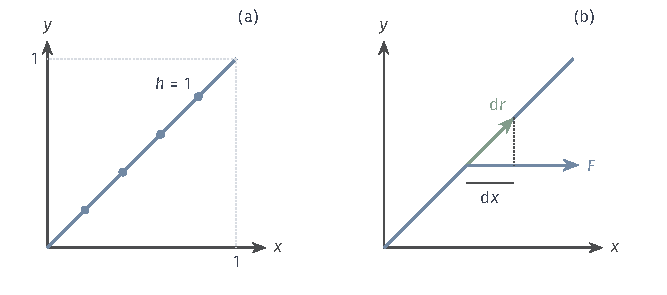
\includegraphics[width=112mm]{figures/01-mathematical-preliminaries-upper/00-shared/tikz/chapter3-concept-processes/line-density-work.pdf}
 \caption{路径均为$\gamma(t)=(t,t)^\top$，$0\leq t\leq1$。(a) 常数线密度$h=1$按弧长累计，得到$\sqrt2$。(b) 常向量场$\bm F=(1,0)^\top$只取位移的水平分量，做功为$1$；图中$\mathrm dx$是$\mathrm d\bm r$的水平投影。相同路径、不同被积对象和权重给出不同积分。}
 \label{fig:analysis-process-line-density-work}
\end{figure}

\subsubsection{积分的基本性质}

下列公式均由内积的线性和一元勒贝格积分的相应性质得到。以下说$\bm F$沿$\gamma$可积，是指定义中的可测性与绝对可积条件成立，因而相应的有向积分有限。前三条说明功对力是线性的，接下来三条说明功怎样随路径的拼接、方向和参数化变化，最后一条估计功的大小。

\paragraph{加法}

若$\bm F$和$\bm G$沿$\gamma$可积，则$\bm F+\bm G$也沿$\gamma$可积，且
\[
 \int_\gamma(\bm F+\bm G)\cdot\mathrm d\bm r
 =\int_\gamma\bm F\cdot\mathrm d\bm r+\int_\gamma\bm G\cdot\mathrm d\bm r.
\]
这里先把两个向量场相加，再与位移取内积。两个力同时作用时，合力做的功等于两个力各自做功之和。

\paragraph{减法}

把$\bm G$换成相反场$-\bm G$，由加法得到
\[
 \int_\gamma(\bm F-\bm G)\cdot\mathrm d\bm r
 =\int_\gamma\bm F\cdot\mathrm d\bm r-\int_\gamma\bm G\cdot\mathrm d\bm r.
\]
可积性保证两个积分都有限，所以可以相减。

\paragraph{数乘}

对实数$c$，有
\[
 \int_\gamma c\bm F\cdot\mathrm d\bm r
 =c\int_\gamma\bm F\cdot\mathrm d\bm r.
\]
力放大$c$倍，功也放大$c$倍；$c<0$时力反向，功变号。路径本身没有改变。

\paragraph{路径拼接}

若$\gamma_1$和$\gamma_2$首尾相接，则
\[
 \int_{\gamma_1*\gamma_2}\bm F\cdot\mathrm d\bm r
 =\int_{\gamma_1}\bm F\cdot\mathrm d\bm r
 +\int_{\gamma_2}\bm F\cdot\mathrm d\bm r.
\]
先走一段再走一段，总功是两段的功之和。因此分段光滑路径可以逐段计算，但每段都必须按这次行进的实际方向参数化。

\paragraph{方向反转}

记反向路径为$\gamma^{-}(u)=\gamma(a+b-u)$，$a\leq u\leq b$，它从$\gamma(b)$出发、沿原路走回$\gamma(a)$。由链式法则，它的速度是$-\gamma'(a+b-u)$，与原速度相反；再用一元换元$t=a+b-u$，得到
\[
 \int_{\gamma^{-}}\bm F\cdot\mathrm d\bm r
 =-\int_\gamma\bm F\cdot\mathrm d\bm r.
\]
顺风骑车时风做正功，沿原路逆风骑回来，风在每一段都做等量的负功。第一类积分反向后不变，因为长度始终非负；有向位移反向则改变符号。
特别地，往返路径$\gamma*\gamma^{-}$上的第二类积分为零，而它的长度是$\gamma$的两倍；示例~\ref{ex:analysis-diagonal-segment-paths}中的$\rho$就是对角线段上的这种往返路径。

\paragraph{重参数化}

若$t=\sigma(u)$为端点相配、严格递增的分段$C^1$微分同胚，则
$(\gamma\circ\sigma)'(u)=\gamma'(\sigma(u))\sigma'(u)$。在参数公式中应用换元$t=\sigma(u)$，得到
\[
 \int_{\gamma\circ\sigma}\bm F\cdot\mathrm d\bm r
 =\int_\gamma\bm F\cdot\mathrm d\bm r.
\]
也就是说，功只取决于经过哪些位置、朝哪个方向经过，与走得快慢无关。
与第一类积分不同，这里乘的是$\sigma'$本身而不是$|\sigma'|$。严格递减的重参数化把路径变成反向路径，换元后积分上下限交换，积分因此变号。重参数化也不改变经过的次数，同一段路重复走两次时，两次的功都会计入。

\paragraph{绝对值不等式}

由积分的三角不等式和Cauchy--Schwarz不等式$|\bm F^\top\bm\tau|\leq\lVert\bm F\rVert_2$可得
\[
 \left|\int_\gamma\bm F\cdot\mathrm d\bm r\right|
 \leq\int_\gamma\lVert\bm F\rVert_2\,\mathrm ds.
\]
功的绝对值不超过力的大小沿路程的累计；当力处处沿前进方向时取等号。若力的大小不超过$M$，路径长为$\ell$，功的绝对值便不超过$M\ell$。
右侧为$+\infty$时，不等式仍成立，但不能用来证明左侧有限。

\subsubsection{积分的计算}

计算第二类路径积分时，按行进方向参数化路径，把场值与速度向量取内积，再做一元积分。与第一类积分相比，这里乘的是速度向量而不是速率。
先用图~\ref{fig:analysis-process-line-density-work}右图中的常力检验这一步骤。
\begin{example}[常力沿对角线段做功]
取常向量场$\bm F=(1,0)^\top$与对角线段$\gamma(t)=(t,t)^\top$，$0\leq t\leq1$。速度为$(1,1)^\top$，被积函数为$1\cdot1+0\cdot1=1$，所以
\[
 \int_\gamma\bm F\cdot\mathrm d\bm r=\int_0^1 1\,\mathrm dt=1.
\]
\end{example}
同一路径的长度为$\sqrt2$。功为$1$而不是$\sqrt2$，是因为水平方向的力只对位移的水平分量做功，而线段的水平跨度是$1$。

再看地面附近的重力。它同样是常向量场，这次让路径任意弯曲。
\begin{example}[重力做功只取决于高度差]
\label{ex:analysis-gravity-work}
设质量为$m$的物体沿分段$C^1$平面路径$\gamma(t)=(x(t),y(t))^\top$，$a\leq t\leq b$，从高度$y(a)$移动到高度$y(b)$，所受重力为$\bm F=(0,-mg)^\top$。被积函数为$\bm F(\gamma(t))^\top\gamma'(t)=-mg\,y'(t)$。在每个光滑段上用一元基本定理，再把各段相加，得到
\[
 \int_\gamma\bm F\cdot\mathrm d\bm r
 =\int_a^b(-mg)\,y'(t)\,\mathrm dt=-mg\bigl(y(b)-y(a)\bigr).
\]
例如质量为$1$千克的物体下降$2$米，即$y(b)-y(a)=-2$，取$g\approx9.8$米每二次方秒，无论沿斜坡还是沿弯曲的滑梯，重力都做功约$9.8\times2=19.6$焦。
\end{example}
被积函数中不含$x'(t)$，水平移动不受重力影响，只有高度变化起作用。这个结果只依赖起点和终点的高度，第~\ref{sec:multivariable-potential-path-independence}节将说明这并非偶然。

对平面图像路径$\gamma(x)=(x,\psi(x))^\top$、$a\leq x\leq b$，其中$\psi$为$C^1$，速度为$(1,\psi'(x))^\top$。$\bm F=(P,Q)^\top$时有
\[
 \int_\gamma\bm F\cdot\mathrm d\bm r
 =\int_a^b\bigl[P(x,\psi(x))+Q(x,\psi(x))\psi'(x)\bigr]\,\mathrm dx.
\]

重力的功与路线无关。下面固定起点和终点，比较两条路线上的功，观察一般向量场是否也如此。
\begin{example}[半圆和直径]
\label{ex:analysis-path-integral-comparison}
取上半圆$\gamma(t)=(\cos t,\sin t)^\top$，$0\leq t\leq\pi$，它从$(1,0)$逆时针走到$(-1,0)$，速度为$(-\sin t,\cos t)^\top$，速率为$1$，故长度$\int_\gamma1\,\mathrm ds=\pi$。另取起点和终点相同的直径$\lambda(t)=(1-2t,0)^\top$，$0\leq t\leq1$，速度为$(-2,0)^\top$。

对常场$(1,0)^\top$，沿上半圆的功为$\int_0^\pi(-\sin t)\,\mathrm dt=-2$，沿直径的功为$\int_0^1(-2)\,\mathrm dt=-2$。两条路线都向左净移动了$2$，水平向右的力在两条路线上做功都是$-2$，恰等于函数$\phi(x,y)=x$在终点与起点的差$-1-1$。

对旋转场$\bm F=(-y,x)^\top$，沿上半圆有$\bm F(\gamma(t))=(-\sin t,\cos t)^\top$，与速度相同，内积为$\sin^2t+\cos^2t=1$，故功为$\pi$：质点一直顺着旋转方向走。
沿直径，$\bm F(\lambda(t))=(0,1-2t)^\top$竖直，而位移水平，内积恒为零，功为$0$。
两条路线端点相同，旋转场做的功却不同。
\end{example}

对常场，功与路线无关；对旋转场，功依赖于路线。沿完整单位圆逆时针一周，质点回到起点，旋转场做功$2\pi$而不是零。图~\ref{fig:analysis-process-rotation-field-paths}画出了旋转场与这两条路线。
\begin{figure}[!htbp]
 \centering
 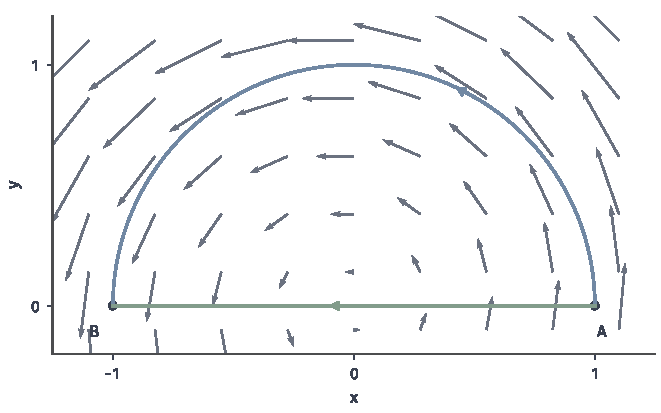
\includegraphics[width=112.0mm]{figures/01-mathematical-preliminaries-upper/00-shared/matplotlib/chapter3-concept-processes/rotation-field-paths.pdf}
 \caption{灰箭头为旋转场$\bm F=(-y,x)^\top$，箭头长度统一缩放为实际场值的$1/4$。两条路径都从$A=(1,0)$到$B=(-1,0)$：蓝色上半圆与场同向，积分为$\pi$；绿色直径上场与位移垂直，积分为零。旋转场处处光滑，端点相同的两条路径上积分仍可不同；下一小节说明势函数给出的路径无关条件。}
 \label{fig:analysis-process-rotation-field-paths}
\end{figure}

\subsection{路径无关与势函数}
\label{sec:multivariable-potential-path-independence}

重力的功只依赖起点和终点的高度，旋转场的功却依赖路线。区别在于：重力的功可以写成某个只依赖位置的量在两端的差，这个量是$-mgy$；旋转场则没有这样的量。
本小节先说明这样的量，即势函数，如何把沿途累计化为端点差；再证明“功与路线无关”反过来也能构造出势函数；最后给出可以直接检查的微分条件，并说明定义域中有洞时，这个条件为什么不再足以保证势函数存在。

\subsubsection{势函数与路径积分}

\paragraph{势函数}

物理中，地面附近质量为$m$的物体在高度$y$处的重力势能为$E_{\mathrm p}(x,y)=mgy$。重力等于势能梯度的相反向量：$-\nabla E_{\mathrm p}=(0,-mg)^\top$。物体下降时势能减少，减少的势能等于重力做的功。
数学中习惯省去负号，取$\phi=-E_{\mathrm p}$，直接要求向量场等于某个标量函数的梯度。
\begin{definition}[势函数]
设$U\subseteq\mathbb R^d$为非空开集，$\bm F:U\to\mathbb R^d$连续。
若存在$\phi\in C^1(U)$使$\bm F=\nabla\phi$，称$\phi$为$\bm F$的\term{势函数}（potential function），称$\bm F$为梯度场，也称保守场。
\end{definition}

梯度指向函数增长最快的方向，所以在梯度非零处，梯度场的箭头指向$\phi$增大的方向，也就是势能$-\phi$减小的方向：重力把物体拉向低处。
例如$\phi(x,y)=x^2+y^2$给出$\bm F(x,y)=(2x,2y)^\top$，箭头从原点向外，因为离原点越远$\phi$越大；常场$(1,0)^\top$的一个势函数是$\phi(x,y)=x$。

给势函数加一个常数，梯度不变，所以势函数不唯一。若$U$还是路径连通的，两个势函数也只能相差一个常数：它们之差的梯度处处为零，路径连通的开集中任意两点都能用域内折线连接，沿折线逐段使用中值公式（定理~\ref{thm:multivariable-scalar-mean-value}），可知这个差在任意两点取值相同。
这与物理中势能的零点可以任选是同一件事：把地面还是桌面取作高度零点，算出的势能差都一样。

“保守”这个名称来自能量守恒。设质量为$m$的质点在力场$\bm F=\nabla\phi$中按牛顿第二定律$m\gamma''(t)=\bm F(\gamma(t))$运动，其中$\gamma$为$C^2$路径。依次用乘积法则、运动方程和链式法则，得到
\[
 \frac{\mathrm d}{\mathrm dt}\Bigl(\tfrac12m\lVert\gamma'(t)\rVert_2^2\Bigr)
 =m\gamma''(t)^\top\gamma'(t)=\nabla\phi(\gamma(t))^\top\gamma'(t)
 =\frac{\mathrm d}{\mathrm dt}\phi(\gamma(t)),
\]
所以动能与势能$-\phi$之和$\frac12m\lVert\gamma'\rVert_2^2-\phi(\gamma)$的导数为零，不随时间变化。最后一个等号已经显示了下面定理的核心：沿路径的功率$\nabla\phi^\top\gamma'$恰是$\phi\circ\gamma$的导数。

\paragraph{路径积分基本定理}

一元基本定理说，导数在区间上的积分等于原函数在两端的差。把势函数与路径复合，得到一元函数$t\mapsto\phi(\gamma(t))$，它的导数恰是第二类路径积分的被积函数，因此一元基本定理直接给出端点差。
直观上，每一小段的功$\nabla\phi^\top\Delta\bm r$近似等于$\phi$在这一小段上的增量，这些增量相加时中间各项逐一抵消，只剩终点值减起点值。
\begin{theorem}[路径积分基本定理]
设$U\subseteq\mathbb R^d$为开集，$\phi\in C^1(U)$，$\gamma:[a,b]\to U$分段$C^1$。则
\begin{equation}
  \int_{\gamma}\nabla\phi\mathbin{\cdot}\mathrm{d}\bm{r}
  =\phi(\gamma(b))-\phi(\gamma(a)).
\label{eq:analysis-line-integral-gradient}
\end{equation}
\end{theorem}
\begin{proof}
在每个光滑参数段$[t_{j-1},t_j]$上，链式法则给出
\[
 (\phi\circ\gamma)'(t)=\nabla\phi(\gamma(t))^\top\gamma'(t).
\]
右侧是连续函数的复合与乘积，在该段上连续，所以对该段使用一元基本定理，得到
$\int_{t_{j-1}}^{t_j}\nabla\phi(\gamma(t))^\top\gamma'(t)\,\mathrm dt=\phi(\gamma(t_j))-\phi(\gamma(t_{j-1}))$。
对$j=1,\dots,n$相加，中间端点的值一正一负逐一抵消，只剩$\phi(\gamma(b))-\phi(\gamma(a))$。
\end{proof}

用势能$E_{\mathrm p}=-\phi$来读，式~\eqref{eq:analysis-line-integral-gradient}说：保守力沿任何路线做的功都等于起点势能减终点势能，即势能的下降量。示例~\ref{ex:analysis-gravity-work}的重力做功就是$\phi(x,y)=-mgy$的情形。

这个定理有两个直接推论。第一，梯度场的积分只依赖端点：两条端点相同的路线，功相同。第二，闭路径的起点与终点重合，所以梯度场沿任意闭路径的积分为零：把书从地上拿到桌上再放回地上，重力在全过程中做的总功为零。
方向反转时端点交换，端点差变号，这与第二类积分的方向反转性质一致。

知道势函数后，计算路径积分不必代入参数。
\begin{example}[用势函数计算沿半圆的积分]
取$\bm F=(2x,2y)^\top$，它的势函数为$\phi(x,y)=x^2+y^2$。路径取示例~\ref{ex:analysis-path-integral-comparison}中的上半圆$\gamma(t)=(\cos t,\sin t)^\top$，$0\leq t\leq\pi$，从$(1,0)$走到$(-1,0)$。由式~\eqref{eq:analysis-line-integral-gradient}，
\[
 \int_\gamma\bm F\cdot\mathrm d\bm r=\phi(-1,0)-\phi(1,0)=1-1=0.
\]
直接代入参数也得到同样结果：$\bm F(\gamma(t))^\top\gamma'(t)=2\cos t\,(-\sin t)+2\sin t\cos t=0$。这个场在圆周上处处沿半径方向，与切线垂直。
\end{example}

第二个推论还可以用来否定势函数的存在。旋转场沿单位圆逆时针一周做功$2\pi\neq0$，所以它在$\mathbb R^2$上没有势函数。

\subsubsection{路径无关的等价判别}

\paragraph{路径无关}

路径积分基本定理说明，有势函数就能推出功与路线无关。要讨论反方向，先把“与路线无关”说准确。比较同一对端点间的不同路线，需要域内任意两点都能用路径连接；对欧氏开集，路径连通时任意两点之间还能选到域内的折线，因而能选到分段光滑路径。
\begin{definition}[路径无关]
设$U\subseteq\mathbb R^d$为非空、开且路径连通的集合，$\bm F:U\to\mathbb R^d$连续。
若对任意$\bm a,\bm b\in U$及域内从$\bm a$到$\bm b$的任意两条分段$C^1$路径，第二类路径积分都相等，称$\bm F$的路径积分与路径无关。
\end{definition}

反方向的想法来自物理中定义势能的办法：选定一个参考点作为势能零点，把力从参考点到某点所做的功取负号，作为该点的势能。只有当这个功与所选路线无关时，这样定义的势能才是一个确定的数。下面的定理说明，路径无关、闭路径积分为零与势函数存在三者等价。
\begin{theorem}[路径无关的等价条件]
设$U\subseteq\mathbb R^d$非空、开且路径连通，$\bm F:U\to\mathbb R^d$连续。下列条件等价：
\begin{enumerate}
 \item 存在$\phi\in C^1(U)$使$\nabla\phi=\bm F$；
 \item $\bm F$的路径积分与路径无关；
 \item 域内每条分段$C^1$闭路径的积分都为零。
\end{enumerate}
\end{theorem}
\begin{proof}
条件1推出条件2，是路径积分基本定理的第一个推论。
条件2推出条件3：设$\gamma$是从$\bm a$出发回到$\bm a$的闭路径。停在$\bm a$不动的常值路径也从$\bm a$到$\bm a$，它的速度为零，积分为零；由路径无关，$\gamma$上的积分也为零。
条件3推出条件2：设$\gamma_1,\gamma_2$都从$\bm a$到$\bm b$。先沿$\gamma_1$走到$\bm b$，再沿$\gamma_2$的反向路径$\gamma_2^-$走回$\bm a$，拼成闭路径$\gamma_1*\gamma_2^-$。由拼接和方向反转性质，
\[
 0=\int_{\gamma_1*\gamma_2^-}\bm F\cdot\mathrm d\bm r
 =\int_{\gamma_1}\bm F\cdot\mathrm d\bm r-\int_{\gamma_2}\bm F\cdot\mathrm d\bm r.
\]

最后由条件2构造势函数。固定参考点$\bm a\in U$，对每个$\bm x\in U$，取域内任意一条从$\bm a$到$\bm x$的分段$C^1$路径，令$\phi(\bm x)$为沿它的积分。路径无关保证这个数不依赖所选路线。
下面计算偏导数。因为$U$开，存在$r>0$使以$\bm x$为中心、半径$r$的球在$U$内。对$0<|h|<r$，到$\bm x+h\bm e_j$的一条路径可以这样选：先沿原来的路径走到$\bm x$，再沿第$j$个坐标方向走线段$t\mapsto\bm x+t\bm e_j$，$t$从$0$到$h$。线段的速度为$\bm e_j$，场与速度的内积是第$j$个分量$F_j$，于是
\[
 \phi(\bm x+h\bm e_j)-\phi(\bm x)
 =\int_0^h F_j(\bm x+t\bm e_j)\,\mathrm dt.
\]
（$h<0$时按有向积分理解。）右侧除以$h$，是$F_j$在这条短线段上的平均值。$F_j$连续，$h\to0$时这个平均值趋于$F_j(\bm x)$，所以$\partial_j\phi(\bm x)=F_j(\bm x)$。
所有偏导数都等于$\bm F$的连续分量，故$\phi\in C^1(U)$且$\nabla\phi=\bm F$，得到条件1。
\end{proof}

证明中的$\phi$正是“从参考点出发做的功”。换一个参考点$\bm a'$，$\phi$只改变一个常数，即从$\bm a'$到$\bm a$的功，这与势能零点可以任选一致。

\subsubsection{势函数存在的微分判别}

\paragraph{交叉偏导相等的必要条件}

路径无关的等价条件把势函数的存在归结为检查所有路径或所有闭路径，实际上无法逐条验证。我们希望找到只需对$\bm F$求导就能检查的条件。
若$\bm F=\nabla\phi$，则$F_j=\partial_j\phi$。当$\bm F$本身是$C^1$时，$\phi$具有连续的二阶偏导数，由定理~\ref{thm:multivariable-mixed-partials}，混合偏导可以交换次序，于是$\bm F$的分量之间必须满足一组关系。
\begin{theorem}[保守场的必要条件]
设$U\subseteq\mathbb R^d$为开集，$\bm F\in C^1(U;\mathbb R^d)$。
若$\bm F=\nabla\phi$，其中$\phi\in C^1(U)$，则对所有$i,j$和$\bm x\in U$，有
\[
 \partial_iF_j(\bm x)=\partial_jF_i(\bm x).
\]
\end{theorem}
\begin{proof}
由$\partial_j\phi=F_j\in C^1(U)$可知$\phi\in C^2(U)$，因此
$\partial_iF_j=\partial_i\partial_j\phi=\partial_j\partial_i\phi=\partial_jF_i$。
\end{proof}

在平面中，记$\bm F=(P,Q)^\top$，条件只有一个：$\partial_xQ=\partial_yP$。差$\partial_xQ-\partial_yP$有清楚的几何含义：它度量向量场在一点附近的旋转程度。

为看出这一点，计算沿一个小正方形边界的环流。设正方形为$[x_0,x_0+\delta]\times[y_0,y_0+\delta]$，按逆时针方向行走。下边向右，贡献$\int_{x_0}^{x_0+\delta}P(x,y_0)\,\mathrm dx$；上边向左，贡献$-\int_{x_0}^{x_0+\delta}P(x,y_0+\delta)\,\mathrm dx$。$P$在上下两边相差约$\partial_yP\,\delta$，所以这两项之和约为$-\partial_yP\cdot\delta\cdot\delta$。同理，右边向上、左边向下，两者的贡献之和约为$\partial_xQ\cdot\delta^2$。
因此小正方形的环流约为$(\partial_xQ-\partial_yP)\,\delta^2$，即单位面积上的环流约为$\partial_xQ-\partial_yP$，下面称它为旋转率。

保守场沿每条闭路径做功为零，小正方形也不例外，所以旋转率必须处处为零，这与上面的必要条件一致。这里只是近似推理；沿区域边界的环流与区域内旋转率的精确关系是Green公式，见定理~\ref{thm:multivariable-green}。

两个例子可以对照。场$(2x,2y)^\top$满足$\partial_xQ=0=\partial_yP$，它确实有势函数$x^2+y^2$。旋转场$(-y,x)^\top$有$\partial_xQ-\partial_yP=1-(-1)=2\neq0$，它在每一点附近都在旋转，由上面的必要条件，它在任何非空开集上都没有势函数。这与单位圆上环流为$2\pi$的计算一致：$2\pi$恰是旋转率$2$乘单位圆盘的面积$\pi$。

\paragraph{星形域上的充分条件}

交叉偏导相等只说明每个小区域内没有旋转，它是局部条件；势函数却要在整个定义域上用一个函数表示。要从局部条件得到全局结论，还需要对定义域本身加条件。

一个便于直接构造的条件是星形：若存在$\bm a\in U$，使从$\bm a$到每个$\bm x\in U$的整条线段都在$U$内，称$U$关于$\bm a$星形。凸开集满足这一条件，整个$\mathbb R^d$也满足。
在星形域上，可以沿用路径无关等价条件证明中“从参考点出发做功”的办法定义势函数，并且总沿直线段从$\bm a$走到$\bm x$。
\begin{theorem}[星形域上势函数的构造]
设$U\subseteq\mathbb R^d$为关于$\bm a$星形的开集，$\bm F\in C^1(U;\mathbb R^d)$，且对所有$i,j$有$\partial_iF_j=\partial_jF_i$。则
\[
 \phi(\bm x)=\int_0^1\bm F(\bm a+t(\bm x-\bm a))^\top(\bm x-\bm a)\,\mathrm dt
\]
属于$C^1(U)$且满足$\nabla\phi=\bm F$。因此$\bm F$的路径积分与路径无关。
\end{theorem}
\begin{proof}
记$\bm z=\bm x-\bm a$。$\phi(\bm x)$是$\bm F$沿线段$t\mapsto\bm a+t\bm z$，$0\leq t\leq1$，的第二类路径积分，因为这条线段的速度恒为$\bm z$。
固定$\bm x$时，这条线段是$U$内的紧集，因而它的一个足够小的紧邻域仍在$U$内；当$\bm x$在一个小范围内变动时，相应线段都留在这个紧邻域中。
$\bm F$及其一阶偏导在紧邻域上连续因而有界，所以被积函数对$x_j$的偏导数有不依赖$t$的上界，可以用式~\eqref{eq:analysis-differentiate-under-integral}在积分号下对$x_j$求导。

被积函数为$\sum_iF_i(\bm a+t\bm z)z_i$。对$x_j$求导时，$z_j$对$x_j$的导数为$1$，$F_i(\bm a+t\bm z)$对$x_j$的导数由链式法则为$t\,\partial_jF_i(\bm a+t\bm z)$，所以偏导数为
\[
 F_j(\bm a+t\bm z)+t\sum_i z_i\partial_jF_i(\bm a+t\bm z).
\]
交叉偏导条件把$\partial_jF_i$换成$\partial_iF_j$，而$\sum_iz_i\partial_iF_j(\bm a+t\bm z)$正是$t\mapsto F_j(\bm a+t\bm z)$的导数，于是
\[
 \begin{aligned}
 F_j(\bm a+t\bm z)+t\sum_i z_i\partial_jF_i(\bm a+t\bm z)
 &=F_j(\bm a+t\bm z)+t\sum_i z_i\partial_iF_j(\bm a+t\bm z)\\
 &=\frac{\mathrm d}{\mathrm dt}\bigl[tF_j(\bm a+t\bm z)\bigr].
 \end{aligned}
\]
对$t$从$0$积分到$1$，由一元基本定理得$\partial_j\phi(\bm x)=1\cdot F_j(\bm a+\bm z)-0=F_j(\bm x)$。
这些偏导连续，所以$\phi\in C^1(U)$；路径无关由前一定理得到。
\end{proof}

用这个构造可以求出一个具体平面场的势函数。
\begin{example}[沿线段构造势函数$x^2y$]
取$\bm F(x,y)=(2xy,x^2)^\top$，即$P=2xy$，$Q=x^2$。它定义在整个平面上，分量都是多项式，属于$C^1$，并且$\partial_yP=2x=\partial_xQ$。整个平面关于$\bm a=\bm0$星形，代入构造公式，
\[
 \phi(x,y)=\int_0^1\bigl[2(tx)(ty)\,x+(tx)^2\,y\bigr]\,\mathrm dt
 =\int_0^13t^2x^2y\,\mathrm dt=x^2y.
\]
直接求导可验证$\nabla\phi=(2xy,x^2)^\top$。于是这个场沿任何从$(0,0)$到$(1,2)$的分段$C^1$路径做功都等于$\phi(1,2)-\phi(0,0)=2$。
\end{example}
星形域上的构造不依赖猜测：交叉偏导相等时，沿线段积分就给出势函数，任意路径上的功随之化为端点差。

\paragraph{穿孔平面上的反例}

星形域的条件不能省略。下面的向量场在原点以外处处满足交叉偏导条件，在穿孔平面上却没有势函数。
\begin{example}[穿孔平面上的涡旋场]
\label{ex:analysis-punctured-plane-vortex}
在穿孔平面$\mathbb R^2\setminus\{\bm0\}$上考虑
\[
 \bm F(x,y)=\left(-\frac{y}{x^2+y^2},\frac{x}{x^2+y^2}\right)^\top ,
\]
记它的两个分量为$P,Q$。它与旋转场$(-y,x)^\top$方向相同，都沿逆时针方向与以原点为圆心的圆相切，但大小改为到原点距离的倒数：离原点越近转得越快，类似于绕一根细涡管旋转的水流。原点处它没有定义。

先检查交叉偏导。由商的求导法则，
\[
 \begin{aligned}
 \partial_yP&=-\frac{(x^2+y^2)-y\cdot2y}{(x^2+y^2)^2}=\frac{y^2-x^2}{(x^2+y^2)^2},\\
 \partial_xQ&=\frac{(x^2+y^2)-x\cdot2x}{(x^2+y^2)^2}=\frac{y^2-x^2}{(x^2+y^2)^2},
 \end{aligned}
\]
两者在穿孔平面上处处相等，所以这个场在原点以外的每一点附近都没有旋转。

再沿单位圆$\gamma(t)=(\cos t,\sin t)^\top$，$0\leq t\leq2\pi$，逆时针走一周。在单位圆上$x^2+y^2=1$，$\bm F(\gamma(t))=(-\sin t,\cos t)^\top$与速度相同，内积为$1$，积分为$2\pi$。
闭路径积分不为零，由路径无关的等价条件，$\bm F$在穿孔平面上没有势函数。
\end{example}

交叉偏导相等这个局部条件，在这里没能给出全局的势函数。这与星形域上的定理并不矛盾：穿孔平面不是星形域，对任一点$\bm a\neq\bm0$，从$\bm a$到$-\bm a$的线段都经过原点。问题出在原点这个洞上，可以从两个角度理解。

第一，局部的势函数是极角。在不含原点的区域上，若能连续地选取点$(x,y)$的极角$\theta$，使$x=r\cos\theta$、$y=r\sin\theta$，其中$r=\sqrt{x^2+y^2}$，则直接求导可得$\nabla\theta=\bm F$。例如在右半平面$x>0$上取$\theta=\arctan(y/x)$，有$\partial_x\theta=-y/(x^2+y^2)$，$\partial_y\theta=x/(x^2+y^2)$。
在更大的区域，即去掉负半轴的平面$\mathbb R^2\setminus\{(x,0)^\top:x\leq0\}$上，取$\theta\in(-\pi,\pi)$，它连续且仍满足$\nabla\theta=\bm F$；这个区域关于$(1,0)$星形，与星形域上的定理一致。

但在整个穿孔平面上无法连续地选取极角：从$(1,0)$出发绕原点逆时针一周回到$(1,0)$，极角连续地增加了$2\pi$，起点和终点处的“势函数值”对不上。单位圆上的积分$2\pi$正是极角的这个增量。
具体地，从$(1,0)$到$(-1,0)$，沿上半圆极角从$0$增加到$\pi$，积分为$\pi$；沿下半圆$(\cos t,-\sin t)^\top$，$0\leq t\leq\pi$，极角从$0$减少到$-\pi$，积分为$-\pi$。两条路线的功相差$2\pi$，恰是绕原点一圈的积分。
不绕原点的闭路径则没有这个问题。例如以$(3,0)$为圆心、半径为$1$的圆整个落在右半平面中，那里$\theta$是势函数，沿它的积分为零。

第二，从小正方形的环流看。交叉偏导相等说明每个小正方形的环流近似为零。若一条闭路径围住的区域整个在定义域内，可以把这个区域划分成许多小正方形；相邻正方形的公共边被沿相反方向各走一次，贡献相互抵消，只剩外边界，于是外边界的环流也为零。这一推理的精确形式就是Green公式（定理~\ref{thm:multivariable-green}），它要求向量场在整个被围区域附近都有定义且连续可微。

单位圆围住的圆盘却包含原点，那里$\bm F$没有定义，无法这样填满。全部旋转都集中在原点这一个洞里。对夹在两条绕原点闭路径之间、不含原点的环形区域作同样的划分，可知两条路径上的环流相等；所以绕原点逆时针一周的简单闭路径，积分都是$2\pi$，而围住的区域不含原点的闭路径，积分为零。

相比之下，星形域上不会出现这样的洞：任何闭路径都可以沿线段向中心点$\bm a$连续收缩而不离开定义域。这从几何上解释了，为什么在星形域上交叉偏导条件已经足以保证势函数存在。

\FloatBarrier

\par\Needspace{10\baselineskip}
\section{曲面积分}
\label{sec:analysis-surface-integration}

路径积分沿一条细线累计：线密度乘弧长得到质量，力与位移的内积累加得到做功。
曲面积分把累计的范围从细线换成薄片，典型问题有两个。
第一个问题是求一张金属薄壳的质量：已知壳上每点每平方米有多少千克，把各小片的“面密度乘面积”加起来即可。
第二个问题是求单位时间内有多少水穿过一张渔网：水在各点有速度，只有垂直于网面的速度分量才把水送到网的另一侧。

两个问题的被积对象不同。
在第一个问题中，被积对象是曲面$S$上的标量函数$h:S\to\mathbb R$，它给出每单位面积的密度，乘面积后相加得到质量、电荷等总量。
在第二个问题中，被积对象是向量场$\bm F:S\to\mathbb R^3$，它在每点给出一个有大小和方向的量；要先取它垂直于曲面的分量，再乘面积相加，得到穿过曲面的\emph{通量}。

两类积分都需要知道曲面上一小片有多大，所以本节先用参数化求出面积元。
通量还需要规定“从哪一侧穿到哪一侧算正”，因此在定义第二类积分之前，还要讨论曲面的定向。
本节的积分都按勒贝格积分理解；参数曲面、面积元和通量的标准构造可参考\scite{math-openstax-calculus3}。

\subsection{参数曲面与面积}

平面区域的面积就是它的二维勒贝格测度。
空间中的曲面一般是弯曲的，不能不经伸缩地摊平成平面区域，所以不能直接用二维测度计算它的面积。
处理地球表面时，人们用经度和纬度两个数确定地面上的一点，这就是一种参数化：用两个参数标记曲面上的点，把曲面上的累计转回二维参数域上计算。
代价是参数域中的面积一般不等于曲面上的实际面积。
经纬度网格上同样大小的格子，在赤道附近和两极附近对应的实际地面面积并不相同，因此每一点都要乘一个面积放大倍数来校正。
本小节先说明怎样的参数化才能描述一张面，再求出这个放大倍数，并证明由此得到的面积不依赖参数的选取。

\subsubsection{曲面的参数化}

\paragraph{正则曲面片}

曲面的参数化是一个向量值映射：输入两个实数$(u,v)$，输出空间中一点的三个坐标。
并不是每个这样的映射都描述一张面。
若改变两个参数时点只沿同一个方向移动，像集可能只是一条曲线；
若不同参数在一块正面积的范围内对应同一些点，按参数累计就会把这块面计算两次。
下面的定义用正则性和单次覆盖两个条件分别排除这两种情况。

\begin{definition}[正则参数曲面片]
\label{def:analysis-regular-surface-patch}
设$E\subseteq\mathbb R^2$是有界闭区域，$E=\overline{E^\circ}$且二维勒贝格测度$m_2(\partial E)=0$。
设$\bm r$在$E$的一个开邻域内是$C^1$映射，写成
\[
 \bm r(u,v)=(x(u,v),y(u,v),z(u,v))^\top\in\mathbb R^3.
\]
若不同参数只有在都属于$\partial E$时才允许表示同一点，
且两个偏导向量$\bm r_u,\bm r_v$在$E^\circ$上处处线性无关，则称$\bm r$为一个正则曲面片的参数化，曲面片记为$S=\bm r(E)$。
参数边界允许产生接缝或退化点；这些边界部分按零曲面面积处理。
\end{definition}

定义中的两个偏导向量有直接的几何含义。
固定$v$而只改变$u$，点$\bm r(u,v)$在曲面上画出一条参数曲线，它的速度向量是$\bm r_u$；
固定$u$而改变$v$得到另一条参数曲线，速度向量是$\bm r_v$。
这里$\bm r_u,\bm r_v$都是三维向量，分别由三个坐标函数对同一个参数求偏导得到，并非某个标量函数的两个偏导数。

两个向量线性无关，是指对任意实数$\alpha,\beta$，
$\alpha\bm r_u+\beta\bm r_v=\bm0$只有在$\alpha=\beta=0$时才成立。
几何上，这表示两个向量不共线，它们张成过该点的一个平面，即曲面的切平面。
若这个条件不成立，像集可能根本不是一张面。

\begin{example}[像集退化为线段的参数映射]
取$E=[0,1]^2$和$\bm r(u,v)=(u+v,0,0)^\top$。
两个偏导向量都等于$(1,0,0)^\top$，因而线性相关。
当$(u,v)$取遍$E$时，$u+v$取遍$[0,2]$，所以像集是$x$轴上的线段$\{(x,0,0)^\top:0\leq x\leq2\}$。
整个正方形被压到这条线段上，像集上没有两个不共线的切方向，也没有面积可言；这个映射不满足正则性条件。
\end{example}

正则性条件排除了这种压扁的映射。
单次覆盖条件处理另一种情况：像集确实是一张面，但被参数重复计数。

\begin{example}[圆柱面的单次覆盖与二重覆盖]
\label{ex:analysis-cylinder-double-cover}
高为$1$的单位圆柱面可以写成
\[
 \bm r(\theta,z)=(\cos\theta,\sin\theta,z)^\top,\qquad z\in[0,1].
\]
偏导向量$\bm r_\theta=(-\sin\theta,\cos\theta,0)^\top$与$\bm r_z=(0,0,1)^\top$处处线性无关，正则性没有问题，需要检查的只有覆盖次数。
若$\theta\in[0,2\pi]$，只有$\theta=0$与$\theta=2\pi$两条边界线表示同一条接缝，这是定义允许的。
若$\theta\in[0,4\pi]$，则对$0<\theta_0<2\pi$和$0<z<1$，点$\bm r(\theta_0,z)$同时由参数域内部的$(\theta_0,z)$和$(\theta_0+2\pi,z)$表示；
按参数累计会把整张柱面计入两次，因此这一参数域不符合定义。
\end{example}

所以不同参数表示同一点的情形只允许出现在参数边界上，形成接缝；参数域内部的点不能与任何其他参数点表示同一点。

本小节反复使用的例子是$\bm r(u,v)=(u,v,u+v)^\top$、$E=[0,1]^2$，下文称它为斜平面片。
它描述平面$z=x+y$上位于单位正方形上方的一块平行四边形，
两个切向量分别为$\bm r_u=(1,0,1)^\top$和$\bm r_v=(0,1,1)^\top$。
前两个坐标就是参数本身，所以不同参数给出不同点；两个切向量不共线，所以它满足正则曲面片的定义。

\paragraph{叉积}

要求曲面的面积，先看参数域中的一个小矩形$[u,u+\Delta u]\times[v,v+\Delta v]$被映成什么形状。
由$\bm r$的可微性，在$\Delta u,\Delta v$很小时有线性近似
\[
 \bm r(u+\Delta u,v+\Delta v)\approx\bm r(u,v)+\bm r_u\Delta u+\bm r_v\Delta v,
\]
其中$\bm r,\bm r_u,\bm r_v$都在$(u,v)$处取值。
于是小矩形的四个顶点近似映为
$\bm r$、$\bm r+\bm r_u\Delta u$、$\bm r+\bm r_v\Delta v$和$\bm r+\bm r_u\Delta u+\bm r_v\Delta v$，
它们正是以$\bm r_u\Delta u$和$\bm r_v\Delta v$为两边的平行四边形的顶点。
所以曲面上的小片近似是切平面内的一个小平行四边形，问题归结为：怎样由两条边向量求平行四边形的面积。

在平面上，两个边向量排成$2\times2$矩阵，其行列式的绝对值就是这个面积。
现在两条边是三维向量，排成的是$3\times2$矩阵，没有行列式可取。
三维空间中常用叉积同时记录这个面积和平行四边形所在平面的垂直方向。
对$\bm a,\bm b\in\mathbb R^3$，定义叉积
\[
 \bm a\times\bm b
 =(a_2b_3-a_3b_2,\ a_3b_1-a_1b_3,\ a_1b_2-a_2b_1)^\top.
\]
例如$(1,0,0)^\top\times(0,1,0)^\top=(0,0,1)^\top$：
$x$轴方向与$y$轴方向的单位向量张成面积为$1$的正方形，叉积是长度为$1$、沿$z$轴的向量。

后面的面积和法向计算要用到叉积的三条性质，下面逐一核对。
第一，叉积垂直于$\bm a$和$\bm b$。直接展开
\[
 \bm a^\top(\bm a\times\bm b)
 =a_1(a_2b_3-a_3b_2)+a_2(a_3b_1-a_1b_3)+a_3(a_1b_2-a_2b_1),
\]
右端六项两两抵消，结果为$0$；对$\bm b$同理。
垂直于同一平面的方向有相反的两个，叉积按右手规则选取其中之一：右手四指从$\bm a$弯向$\bm b$时，拇指指向$\bm a\times\bm b$。

第二，叉积的长度等于$\bm a,\bm b$张成的平行四边形的面积。
把两边按分量展开，可以验证Lagrange恒等式
\[
 \lVert\bm a\times\bm b\rVert_2^2
 =\lVert\bm a\rVert_2^2\lVert\bm b\rVert_2^2-(\bm a^\top\bm b)^2.
\]
记$\theta\in[0,\pi]$为两向量的夹角，则$\bm a^\top\bm b=\lVert\bm a\rVert_2\lVert\bm b\rVert_2\cos\theta$，
代入得$\lVert\bm a\times\bm b\rVert_2=\lVert\bm a\rVert_2\lVert\bm b\rVert_2\sin\theta$。
以$\bm a$为底边时，平行四边形的高是$\lVert\bm b\rVert_2\sin\theta$，所以叉积长度正是“底乘高”。
特别地，叉积为零当且仅当两向量共线，即平行四边形退化为线段或一点。

第三，叉积对每个因子都是线性的，交换两个因子的次序会变号：从定义式直接看出$\bm b\times\bm a=-\bm a\times\bm b$，特别地$\bm a\times\bm a=\bm0$。
这与右手规则一致：交换次序后四指的弯曲方向相反，拇指也随之反向。

把这些性质用到小平行四边形上。由线性，
$(\bm r_u\Delta u)\times(\bm r_v\Delta v)=(\bm r_u\times\bm r_v)\Delta u\Delta v$；
再由第二条性质，小曲面片的面积近似为
\[
 \lVert\bm r_u\times\bm r_v\rVert_2\,\Delta u\,\Delta v.
\]
因此$\lVert\bm r_u\times\bm r_v\rVert_2$就是参数化在该点的面积放大倍数：参数域中面积为$\Delta u\Delta v$的小块，
在曲面上变成面积约为这个倍数乘$\Delta u\Delta v$的小片。
同样由第二条性质，正则性条件“两个切向量线性无关”可以等价地写成$\bm r_u\times\bm r_v\ne\bm0$，即放大倍数处处为正。

平面情形可以用来核对这个倍数。若曲面就在平面$z=0$内，即$\bm r(u,v)=(x(u,v),y(u,v),0)^\top$，
则$\bm r_u\times\bm r_v=(0,0,x_uy_v-x_vy_u)^\top$，其长度正是映射$(u,v)\mapsto(x,y)$的Jacobian行列式的绝对值。
这与第~\ref{sec:multivariable-change-variables}节换元公式中的面积权重$|\det\bm J_T|$一致；叉积长度是这个权重在三维空间中的推广。

\subsubsection{曲面面积的表示}

\paragraph{面积元与面积测度}

把参数域分成许多小矩形，由小平行四边形的面积近似，每块在曲面上的像的面积约为放大倍数乘参数面积，曲面的总面积约为这些乘积之和。
小矩形越细，线性近似越准确，求和的极限就是放大倍数在参数域上的积分。

这里直接把这个积分取作曲面面积的定义，而不像弧长那样用内接折线长度的上确界来定义，因为曲面上的类似做法会失败。
在一段有限高的圆柱面上，可以构造顶点都在柱面上的三角形网格（称为Schwarz灯笼），
使网格越来越细，三角形与柱面的夹角却不趋于零，三角形总面积可以趋于无穷。
用切平面上的平行四边形近似则不会出现这种问题，因为每个小平行四边形都贴着切平面。

\begin{definition}[曲面面积测度]
\label{def:analysis-surface-area-measure}
在上述曲面片上，记$J_S(u,v)=\lVert\bm r_u\times\bm r_v\rVert_2$。
若$A\subseteq S$的原像$\bm r^{-1}(A)\cap E$勒贝格可测，则称$A$为曲面可测集，定义
\[
 \sigma_S(A)=\iint_E\bm1_A(\bm r(u,v))J_S(u,v)\,\mathrm du\,\mathrm dv.
\]
曲面面积元记为$\mathrm dS$，参数表示为
\[
 \mathrm dS=J_S(u,v)\,\mathrm du\,\mathrm dv,
 \qquad \operatorname{area}(S)=\sigma_S(S).
\]
\end{definition}

$\sigma_S(A)$先找出$A$在参数域中的原像，再把原像上每一点的放大倍数积起来。
这样得到的确实是一个测度。原像运算保持集合的补、交和可数并，所以曲面可测集构成$\sigma$代数。
对两两不交的曲面可测集，并集的指示函数等于各指示函数之和；$\sigma_S$由非负函数的勒贝格积分给出，由单调收敛定理（定理~\ref{thm:analysis-monotone-convergence}）可以逐项积分，所以$\sigma_S$可数可加。

$J_S$在紧集$E$上连续，因而有界；又$m_2(E)<\infty$，故曲面片的面积有限。
参数边界的二维测度为零，在定义式中不贡献面积；边界接缝上的点即使被两个参数表示，也只位于零测集上，不会造成正面积的重复累计。

用这一定义计算斜平面片的面积，并用初等几何核对结果。

\begin{example}[斜平面片的面积]
\label{ex:analysis-tilted-plane-area}
对斜平面片$\bm r(u,v)=(u,v,u+v)^\top$、$E=[0,1]^2$，按叉积的定义计算
\[
 \begin{aligned}
 \bm r_u\times\bm r_v
 &=(1,0,1)^\top\times(0,1,1)^\top\\
 &=(0\cdot1-1\cdot1,\ 1\cdot0-1\cdot1,\ 1\cdot1-0\cdot0)^\top
 =(-1,-1,1)^\top,
 \end{aligned}
\]
故$J_S=\lVert(-1,-1,1)^\top\rVert_2=\sqrt3$处处成立，曲面面积为
\[
 \operatorname{area}(S)=\int_0^1\int_0^1\sqrt3\,\mathrm du\,\mathrm dv=\sqrt3.
\]
用初等几何核对：两条边$\bm r_u,\bm r_v$的长度都是$\sqrt2$，内积为$1$，夹角余弦为$1/2$，即夹角为$60^\circ$；
平行四边形面积为$\sqrt2\cdot\sqrt2\cdot\sin60^\circ=\sqrt3$，与积分结果相同。
\end{example}

参数正方形的面积只有$1$，曲面片的面积却是$\sqrt3$：每个参数小块都被放大$\sqrt3$倍。
图~\ref{fig:analysis-process-surface-area-stretch}将参数小块与实际斜面小块对应起来，显示叉积长度校正的是哪一个面积。
\begin{figure*}[!htbp]
 \centering
 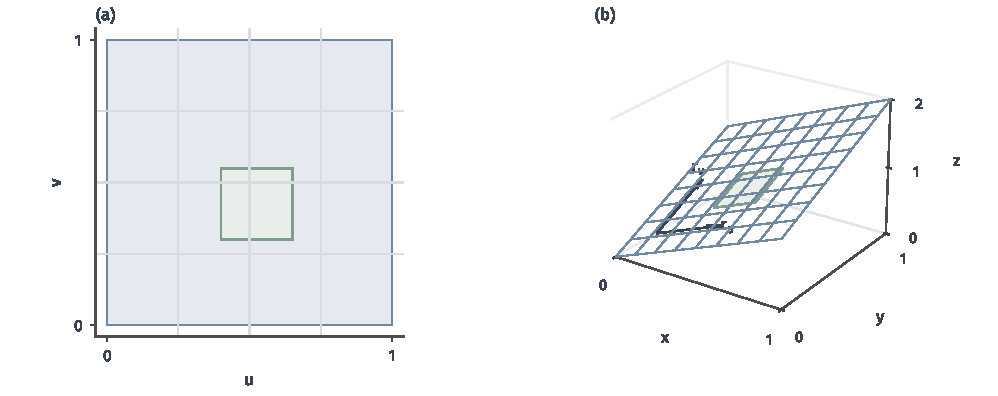
\includegraphics[width=169.0mm]{figures/01-mathematical-preliminaries-upper/00-shared/matplotlib/chapter3-concept-processes/surface-area-stretch.pdf}
 \caption{参数化$r(u,v)=(u,v,u+v)^\top$把单位正方形映为斜平面片，绿色块为同一参数子区间及其像。两切向量$r_u=(1,0,1)^\top$、$r_v=(0,1,1)^\top$在右侧按$0.4$倍画出，叉积长度为$\sqrt3$。每个参数面积都放大$\sqrt3$倍，故不能把$\mathrm du\,\mathrm dv$直接当成$\mathrm dS$。}
 \label{fig:analysis-process-surface-area-stretch}
\end{figure*}

\paragraph{重参数化}

同一张面可以用不同参数标记。
面积是曲面本身的属性，不应随标记方式改变；先在斜平面片上核对一次具体的换参数。

\begin{example}[拉伸一个参数不改变面积]
\label{ex:analysis-stretched-parameter-area}
在斜平面片中令$u=2\xi$，则
\[
 \widetilde{\bm r}(\xi,v)=(2\xi,v,2\xi+v)^\top,\qquad (\xi,v)\in[0,1/2]\times[0,1]
\]
描述同一块平行四边形，新参数域的面积只有$1/2$。
另一方面，$\widetilde{\bm r}_\xi=(2,0,2)^\top=2\bm r_u$，$\widetilde{\bm r}_v=\bm r_v$，由叉积的线性，
$\widetilde{\bm r}_\xi\times\widetilde{\bm r}_v=2(\bm r_u\times\bm r_v)=2(-1,-1,1)^\top$，放大倍数为$2\sqrt3$。
因此
\[
 \int_0^1\int_0^{1/2}2\sqrt3\,\mathrm d\xi\,\mathrm dv=\sqrt3,
\]
与示例~\ref{ex:analysis-tilted-plane-area}的结果相同。
\end{example}

参数域缩小一半，每点的放大倍数恰好加倍，两者相互抵消。
下面的定理说明，这种抵消对一般的单次覆盖换参数都成立。

\begin{theorem}[重参数化下的面积元]
\label{thm:analysis-surface-reparameterization}
设$\bm r:E\to S$是正则曲面片的参数化，$T:\widetilde E\to E$是参数域之间的双射，
在$\widetilde E$的一个开邻域内为$C^1$映射，并且限制在$\widetilde E^\circ$上是到$E^\circ$的$C^1$微分同胚。
若$\widetilde{\bm r}=\bm r\circ T$仍满足曲面片条件，则
\[
 \begin{aligned}
 \widetilde{\bm r}_\xi\times\widetilde{\bm r}_\eta
 &=\det\bm J_T\,(\bm r_u\times\bm r_v)\circ T,\\
 \widetilde J_S&=(J_S\circ T)|\det\bm J_T|.
 \end{aligned}
\]
两组参数由此给出同一面积测度。
\end{theorem}

\begin{proof}
记$T(\xi,\eta)=(u(\xi,\eta),v(\xi,\eta))$。
链式法则给出$\widetilde{\bm r}_\xi=\bm r_u u_\xi+\bm r_v v_\xi$和
$\widetilde{\bm r}_\eta=\bm r_u u_\eta+\bm r_v v_\eta$，其中右端各量在$T(\xi,\eta)$处取值。
用叉积对每个因子的线性展开，得到四项：
\[
 \begin{aligned}
 \widetilde{\bm r}_\xi\times\widetilde{\bm r}_\eta
 &=u_\xi u_\eta(\bm r_u\times\bm r_u)+u_\xi v_\eta(\bm r_u\times\bm r_v)\\
 &\quad{}+v_\xi u_\eta(\bm r_v\times\bm r_u)\\
 &\quad{}+v_\xi v_\eta(\bm r_v\times\bm r_v).
 \end{aligned}
\]
由$\bm a\times\bm a=\bm0$，第一、四项为零；交换叉积次序会变号，即$\bm r_v\times\bm r_u=-\bm r_u\times\bm r_v$，于是第三项可与第二项合并。因此
\[
 \widetilde{\bm r}_\xi\times\widetilde{\bm r}_\eta
 =(u_\xi v_\eta-v_\xi u_\eta)(\bm r_u\times\bm r_v)\circ T,
\]
括号内正是$\det\bm J_T$，这就是第一式；两边取长度得到第二式。
对任一可测集$A\subseteq S$，新参数下的面积为
\[
 \iint_{\widetilde E}\bm1_A(\bm r(T(\xi,\eta)))\,J_S(T(\xi,\eta))\,|\det\bm J_T(\xi,\eta)|\,\mathrm d\xi\,\mathrm d\eta.
\]
在$\widetilde E^\circ$上应用二维换元公式~\eqref{eq:measurable-change-variables}，并注意参数边界为零测集，
它等于$\iint_E\bm1_A(\bm r(u,v))J_S(u,v)\,\mathrm du\,\mathrm dv$，即原参数下的面积。
\end{proof}

几何上，这个证明把两步面积放大接在一起：新参数的小方块先由$T$映成原参数域中面积约为$|\det\bm J_T|$倍的小块，
这个小块再由$\bm r$映到曲面，面积又乘$J_S$。
二维换元公式恰好把第一步的倍数吸收掉，所以只剩下曲面本身的面积。
在示例~\ref{ex:analysis-stretched-parameter-area}中，$T(\xi,v)=(2\xi,v)$，$\det\bm J_T=2$，这正是放大倍数加倍的来源。

行列式的绝对值保证面积非负；行列式本身的符号则记录参数次序是否翻转。
例如在斜平面片上交换两个参数，令$T(\xi,\eta)=(\eta,\xi)$，即$\widetilde{\bm r}(\xi,\eta)=\bm r(\eta,\xi)=(\eta,\xi,\xi+\eta)^\top$，则$\det\bm J_T=-1$，
叉积由$(-1,-1,1)^\top$变为$(1,1,-1)^\top$，长度不变而方向相反。
面积不使用这个方向，后面选取通量的法向时则要用到它。

定理还要求$T$是双射。若参数在正面积的范围内重复覆盖，参数积分就会重复累计。
示例~\ref{ex:analysis-cylinder-double-cover}中，$\bm r_\theta\times\bm r_z=(\cos\theta,\sin\theta,0)^\top$，$J_S=1$；
$\theta\in[0,2\pi]$时参数积分给出柱面面积$2\pi$，$\theta\in[0,4\pi]$时却给出$4\pi$，不能当作单次覆盖的曲面面积。

\paragraph{分片曲面}

有些曲面不能用一张正则曲面片描述。单位立方体的表面由六个正方形组成，棱上没有切平面。
球面虽然可以用一张球坐标参数片覆盖（两极位于参数边界上，切向量在那里退化），也常分成上下两个半球分别处理。
本节只处理有限分片的情形：把曲面写成有限张正则曲面片的并，各片内部不重叠，交接部分在相邻曲面片中面积均为零，
整个曲面的面积测度由各片的面积测度相加。

例如立方体表面的面积就是六个单位正方形的面积之和$6$，十二条棱的面积为零，不需要在接缝上另加一项。
后面的两类曲面积分同样可以逐片计算再相加。
无界曲面，或不能这样由有限张正则曲面片覆盖的曲面，还需另外处理覆盖和可积性条件。

\subsection{第一类曲面积分}

有了面积测度，就可以回到本节开头的第一个问题：在曲面上累计一个标量密度。
这类积分只用到小片的面积，不涉及方向。

\subsubsection{积分的定义和可积性}

\paragraph{按面积的积分}

设一张薄金属壳占据曲面$S$，在点$\bm x$附近每单位面积的质量为$h(\bm x)$（单位如千克每平方米）。
把壳分成许多小片$S_j$，在每片内取一点$\bm x_j$。
若每片很小，片内面密度近似为常数$h(\bm x_j)$，这一片的质量约为$h(\bm x_j)\,\sigma_S(S_j)$。
把各片质量相加，再让分割越来越细，就得到面密度对面积测度的积分。
带电薄壳上的电荷量、涂层表面的涂料用量都是同一种累计。
下面的定义直接使用面积测度上的勒贝格积分，因此不仅适用于连续密度，也适用于有跳跃或仅可测的密度。

\begin{definition}[第一类曲面积分]
\label{def:analysis-scalar-surface-integral}
设$h$是$S$上的可测标量函数。
当$h\geq0$时，定义它的\term{第一类曲面积分}（scalar surface integral）为
\begin{equation}
 \int_Sh\,\mathrm dS
 =\iint_Eh(\bm r(u,v))J_S(u,v)\,\mathrm du\,\mathrm dv.
 \label{eq:analysis-scalar-surface-integral}
\end{equation}
该值允许为$+\infty$。一般实值$h$在$\int_S|h|\,\mathrm dS<\infty$时称为曲面可积，
其积分按正、负部分之差定义，仍满足上式。
\end{definition}

式~\eqref{eq:analysis-scalar-surface-integral}右端的计算顺序是：用参数找到曲面上的点，读出该点的密度，乘该点的面积放大倍数，再在参数域上积分。
定理~\ref{thm:analysis-surface-reparameterization}表明两组单次覆盖的正则参数给出同一面积测度，所以换用另一组参数不会改变积分值。
取$h=1$得到面积，取非负面密度得到质量。
例如在斜平面片上，常数密度$h=2$给出
\[
 \int_S2\,\mathrm dS=\int_0^1\int_0^1 2\sqrt3\,\mathrm du\,\mathrm dv=2\sqrt3,
\]
即面积为$\sqrt3$、每单位面积重$2$的薄片，总质量为$2\sqrt3$。

除了总量，第一类积分还给出曲面上的平均值。设$0<\operatorname{area}(S)<\infty$且$h$曲面可积，则
\[
 \frac1{\operatorname{area}(S)}\int_Sh\,\mathrm dS
\]
是$h$按面积加权的平均。若$h$表示地球表面各点的气温，这个量就是全球表面平均气温：
每块地面按其实际面积参与平均，而不是按经纬度网格的格子数参与平均。

质量和平均值都只依赖每小片的大小，不依赖从哪一侧看曲面，所以把曲面的朝向反过来，第一类积分不变。

\paragraph{可积性的要求}

对一般实值函数，第一类积分要求绝对积分有限。
由定义，$h$曲面可积当且仅当$h\circ\bm r$在$E$上可测，且
\[
 \iint_E|h(\bm r(u,v))|J_S(u,v)\,\mathrm du\,\mathrm dv<\infty,
\]
也就是函数大小乘面积权重后在参数域上的累计有限。
连续函数是一个便于验证的充分情形：$S=\bm r(E)$紧致，连续的$h$在其上有界，
因而$\int_S|h|\,\mathrm dS\leq \sup_S|h|\,\sigma_S(S)<\infty$。

可测性本身并不保证绝对积分有限。
函数在某点附近无界时，要比较它增大的速度与该点附近面积缩小的速度。
下面以球面上到北极点距离的负幂为例，先用环带面积估计可积的阈值。

\begin{example}[球面上距离负幂的可积阈值]
\label{ex:analysis-sphere-distance-power}
设$S$是以原点为中心、半径为$R$的球面，$\bm N=(0,0,R)^\top$为北极点，$\alpha>0$，
令$h(\bm x)=\lVert\bm x-\bm N\rVert_2^{-\alpha}$（$\bm N$处任取一值，单点的面积为零）。
在到北极点的距离不小于某个正数的部分，$h$有界，所以问题只在北极点附近。
到北极点距离为$\rho$的点组成一个圆，$\rho$很小时它的周长约为$2\pi\rho$；所以距离介于$\rho$与$\rho+\Delta\rho$之间的环带面积约为$2\pi\rho\,\Delta\rho$，而$h$在环带上约为$\rho^{-\alpha}$。
因此北极附近的累计与
\[
 \int_0^\delta\rho^{-\alpha}\cdot2\pi\rho\,\mathrm d\rho
 =2\pi\int_0^\delta\rho^{1-\alpha}\,\mathrm d\rho
\]
同时有限或同时发散，其中$\delta>0$是某个小数。
右端在$\alpha<2$时有限、在$\alpha\geq2$时发散，所以按这一估计，$h$曲面可积当且仅当$\alpha<2$。
示例~\ref{ex:analysis-sphere-distance-power-exact}将用球坐标精确计算这个积分，验证这里的估计。
\end{example}

这一阈值与平面上$\lVert\bm x\rVert_2^{-p}$在单位圆盘上可积当且仅当$p<2$的结论（第~\ref{sec:multivariable-riemann-lebesgue}节）相同。
原因是曲面在小范围内近似于切平面，环带面积与平面圆环面积按同样的方式随半径变化。
取$\alpha=1$：电学中点电荷的电势与距离成反比，若点电荷位于北极点，电势在球面上的积分有限。

这些条件都相对于曲面面积而言，而非三维体积测度。
曲面在三维空间中的体积为零，若对三维勒贝格测度积分，任何函数在曲面上的积分都是零；面积测度正是为了给这种零体积集合赋予有意义的大小。

\subsubsection{积分的性质}

第一类曲面积分是面积测度上的勒贝格积分，因此勒贝格积分的线性、可加性和单调性都直接适用。
以下各条均以相应函数曲面可积为前提，并分别说明它们在薄壳质量或电荷上的含义。

\paragraph{加法}

对曲面可积的$h,k$，$h+k$也可积，而且
\[
 \int_S(h+k)\,\mathrm dS=\int_Sh\,\mathrm dS+\int_Sk\,\mathrm dS.
\]
可积性由$|h+k|\leq|h|+|k|$得到，等式来自标量勒贝格积分的加法性质。
若薄壳由两层材料叠成，面密度分别为$h$和$k$，这个等式表示总质量等于两层质量之和。

\paragraph{减法}

对曲面可积的$h,k$，$h-k$也可积，而且
\[
 \int_S(h-k)\,\mathrm dS=\int_Sh\,\mathrm dS-\int_Sk\,\mathrm dS.
\]
这里$|h-k|\leq|h|+|k|$保证绝对可积，等式来自标量勒贝格积分的减法性质。

\paragraph{数乘}

对实数$c$和曲面可积的$h$，$ch$曲面可积，且
\[
 \int_Sch\,\mathrm dS=c\int_Sh\,\mathrm dS.
\]
因为$|ch|=|c||h|$，绝对积分仍有限；等式来自标量勒贝格积分的数乘性质。
例如把面密度的单位从千克每平方米换成克每平方米，相当于$c=1000$，总质量的数值也乘$1000$。

\paragraph{曲面分割的可加性}

若可测子集$A_j\subseteq S$（$j=1,2,\ldots$）两两不交，且$h$在$S$上曲面可积，则
\[
 \int_{\bigcup_{j=1}^\infty A_j}h\,\mathrm dS
 =\sum_{j=1}^\infty\int_{A_j}h\,\mathrm dS.
\]
右侧级数绝对收敛，因为其各项绝对值之和不超过$\int_S|h|\,\mathrm dS$；等式来自勒贝格积分对积分区域的可数可加性。
它表示把薄壳切成若干块分别称重，再把重量相加，与整块称重的结果相同。
有限分片曲面的逐片求和是这一性质的特例；各片仅在零面积接缝上相交，也不影响等式。

\paragraph{单调性}

若曲面可积的$h,k$满足$h\leq k$在曲面面积意义下几乎处处成立，则
\[
 \int_Sh\,\mathrm dS\leq\int_Sk\,\mathrm dS.
\]
因为$k-h$几乎处处非负，其积分非负，应用减法公式即可得到这一不等式。
这里的“几乎处处”允许忽略零曲面面积的集合，例如有限条曲线；它不以三维体积衡量例外集合，否则整张曲面都会被忽略。

\paragraph{绝对值不等式}

对任一曲面可积的$h$，将单调性应用于$-|h|\leq h\leq|h|$得到
\[
 \left|\int_Sh\,\mathrm dS\right|\leq\int_S|h|\,\mathrm dS.
\]
当$h$有正有负时，例如表示正负电荷的面密度，左端是净电荷的大小，右端是不计符号的电荷总量；
正负部分会相互抵消，所以净量不超过总量。

\subsubsection{积分的计算}

计算第一类曲面积分分三步：选一个单次覆盖的正则参数化，把$h$与参数化复合，再乘叉积的长度后在参数域上积分。
最常见的两种参数化是函数图像和球坐标。

若曲面是函数$z=\psi(x,y)$在区域$D$上的图像，其中$D$满足定义~\ref{def:analysis-regular-surface-patch}对参数域的要求，$\psi$在$D$的开邻域内为$C^1$，就可以取
$\bm r(x,y)=(x,y,\psi(x,y))^\top$。此时$\bm r_x=(1,0,\psi_x)^\top$、$\bm r_y=(0,1,\psi_y)^\top$，按叉积公式计算得
\[
 \begin{aligned}
 \bm r_x\times\bm r_y
 &=(0\cdot\psi_y-\psi_x\cdot1,\ \psi_x\cdot0-1\cdot\psi_y,\ 1\cdot1-0\cdot0)^\top\\
 &=(-\psi_x,-\psi_y,1)^\top.
 \end{aligned}
\]
叉积的第三分量恒为$1$，所以图像参数化处处正则；前两个坐标就是参数本身，所以单次覆盖也自动成立。
于是对曲面可积的$h$有
\[
 \int_Sh\,\mathrm dS
 =\iint_Dh(x,y,\psi(x,y))\sqrt{1+\psi_x^2+\psi_y^2}\,\mathrm dx\,\mathrm dy.
\]

根号的几何意义如下。记$\gamma$为法向$(-\psi_x,-\psi_y,1)^\top$与$z$轴的夹角，
则$\cos\gamma=1/\sqrt{1+\psi_x^2+\psi_y^2}$。
一块与水平面成角$\gamma$的小平面片，竖直投影到$xy$平面上时面积缩小为原来的$\cos\gamma$倍；
反过来，由投影面积$\mathrm dx\,\mathrm dy$恢复实际面积，就要除以$\cos\gamma$，即乘上这个根号。
曲面越陡，根号越大。例如$z=ax+by+c$在单位圆盘上方的部分，根号处处等于$\sqrt{1+a^2+b^2}$，面积为
$\pi\sqrt{1+a^2+b^2}$；$a=b=0$时它就是水平圆盘的面积$\pi$。
若曲面不能单值地投影到同一坐标平面，例如整张球面在每个$(x,y)$上方有两点，则需换参数化或分片。

半径$R>0$的球面可以取参数
\[
 \begin{gathered}
 \bm r(\varphi,\theta)
 =(R\sin\varphi\cos\theta,R\sin\varphi\sin\theta,R\cos\varphi)^\top,\\
 0\leq\varphi\leq\pi,\quad 0\leq\theta\leq2\pi,
 \end{gathered}
\]
其中$\varphi$是与北极方向的夹角，$\theta$是绕$z$轴转过的角度。求偏导得
\[
 \begin{aligned}
 \bm r_\varphi&=(R\cos\varphi\cos\theta,R\cos\varphi\sin\theta,-R\sin\varphi)^\top,\\
 \bm r_\theta&=(-R\sin\varphi\sin\theta,R\sin\varphi\cos\theta,0)^\top.
 \end{aligned}
\]
这两个向量的内积为零，长度分别为$R$和$R\sin\varphi$；由叉积长度公式（夹角为$\pi/2$），叉积长度为$R^2\sin\varphi$。
这个结果也可以直接看出：$\varphi$增加$\Delta\varphi$时，点沿经线走过约$R\Delta\varphi$；
$\theta$增加$\Delta\theta$时，点沿半径为$R\sin\varphi$的纬线圈走过约$R\sin\varphi\,\Delta\theta$。
小片近似为以这两个长度为边的矩形。靠近两极时纬线圈变小，同样的$\Delta\theta$对应的面积也变小。

在参数域内部$0<\varphi<\pi$、$0<\theta<2\pi$上$\sin\varphi>0$，参数化正则且单次覆盖；
两极与经线接缝来自参数边界，面积为零，不需要单独处理。
先用这个参数化求球面面积。

\begin{example}[球面的面积]
\label{ex:analysis-sphere-area}
对半径为$R$的球面，球坐标参数的面积放大倍数为$J_S=R^2\sin\varphi$，被积函数非负，可以逐次积分：
\[
 \operatorname{area}(S)
 =\int_0^{2\pi}\int_0^\pi R^2\sin\varphi\,\mathrm d\varphi\,\mathrm d\theta
 =2\pi R^2\bigl[-\cos\varphi\bigr]_0^\pi
 =4\pi R^2.
\]
\end{example}

球坐标也能把示例~\ref{ex:analysis-sphere-distance-power}中的环带估计变成精确计算。

\begin{example}[球面上距离负幂积分的精确值]
\label{ex:analysis-sphere-distance-power-exact}
沿用示例~\ref{ex:analysis-sphere-distance-power}的记号，$\bm N=(0,0,R)^\top$。在球坐标下
\[
 \lVert\bm r(\varphi,\theta)-\bm N\rVert_2^2
 =R^2\sin^2\varphi+R^2(1-\cos\varphi)^2
 =2R^2(1-\cos\varphi)
 =4R^2\sin^2\tfrac\varphi2,
\]
所以到北极点的距离为$s=2R\sin(\varphi/2)$。
它是$\varphi\in[0,\pi]$上递增的$C^1$函数，把$[0,\pi]$映为$[0,2R]$，且$\mathrm ds=R\cos(\varphi/2)\,\mathrm d\varphi$，从而
\[
 R^2\sin\varphi\,\mathrm d\varphi
 =2R^2\sin\tfrac\varphi2\cos\tfrac\varphi2\,\mathrm d\varphi
 =s\,\mathrm ds.
\]
被积函数非负，先对$\theta$积分得到因子$2\pi$，再换元：
\[
 \int_S\lVert\bm x-\bm N\rVert_2^{-\alpha}\,\mathrm dS
 =2\pi\int_0^\pi\Bigl(2R\sin\tfrac\varphi2\Bigr)^{-\alpha}R^2\sin\varphi\,\mathrm d\varphi
 =2\pi\int_0^{2R}s^{1-\alpha}\,\mathrm ds.
\]
当$0<\alpha<2$时，积分值为$2\pi(2R)^{2-\alpha}/(2-\alpha)$；当$\alpha\geq2$时，积分为$+\infty$。
\end{example}

精确结果与环带估计给出同一个阈值。
对$\theta$积分后，面积元成为$2\pi s\,\mathrm ds$，所以到北极点距离介于$s$与$s+\Delta s$之间的环带面积约为$2\pi s\,\Delta s$；这一规律不只在北极附近成立，在整张球面上都成立。

面积权重在求平均时同样不可缺少，下面以上半球面上的平均高度为例。

\begin{example}[上半球面的平均高度]
\label{ex:analysis-hemisphere-average-height}
取上半球面$0\leq\varphi\leq\pi/2$，高度函数$h(\bm x)=z$。
由$J_S=R^2\sin\varphi$，上半球面面积为$2\pi R^2\int_0^{\pi/2}\sin\varphi\,\mathrm d\varphi=2\pi R^2$，而
\[
 \int_Sz\,\mathrm dS
 =\int_0^{2\pi}\int_0^{\pi/2}R\cos\varphi\cdot R^2\sin\varphi\,\mathrm d\varphi\,\mathrm d\theta
 =2\pi R^3\cdot\frac12=\pi R^3,
\]
所以按面积加权的平均高度为$\pi R^3/(2\pi R^2)=R/2$。
若改为在参数矩形$[0,\pi/2]\times[0,2\pi]$上按参数面积平均，则得到
\[
 \frac1{(\pi/2)\cdot2\pi}\int_0^{2\pi}\int_0^{\pi/2}R\cos\varphi\,\mathrm d\varphi\,\mathrm d\theta
 =\frac{2R}{\pi}\approx0.64R.
\]
\end{example}

两种平均不同，是因为同样大小的参数格子在北极附近只对应很小的面积：按参数平均会过多计入北极附近的高点，因而高估平均高度。
面积权重$R^2\sin\varphi$正是为了按实际面积而不是按参数格子求平均。

\subsection{第二类曲面积分}

现在回到本节开头的第二个问题：向量场穿过曲面的总量。
面积测度只给出小片的大小；要说“穿过”，还必须先规定曲面的哪一侧算出发侧、哪一侧算到达侧。
因此本小节先讨论曲面的定向，再定义通量。

\subsubsection{曲面的定向}

\paragraph{单位法向量}

在正则点，切平面有两个互相相反的单位法向量，分别指向曲面的两侧。
选定其中一个，就约定：从曲面上背向它的一侧穿到它所指的一侧，算作正向穿越。
参数化的叉积给出一个自然的局部选择：在$E^\circ$上令
\[
 \bm n(\bm r(u,v))
 =\frac{\bm r_u\times\bm r_v}{\lVert\bm r_u\times\bm r_v\rVert_2}.
\]
由叉积的性质，这个向量长度为$1$，并且垂直于两个参数方向，即垂直于切平面；交换$u,v$的次序会把它反转。

在斜平面片上，这个公式给出$(-1,-1,1)^\top/\sqrt3$，它的第三分量为正，指向平面的上方。
在球坐标参数下，直接计算可得
\[
 \bm r_\varphi\times\bm r_\theta
 =R^2\sin\varphi\,(\sin\varphi\cos\theta,\sin\varphi\sin\theta,\cos\varphi)^\top
 =R\sin\varphi\,\bm r(\varphi,\theta).
\]
在参数域内部，叉积是位置向量的正数倍，所以单位法向为$\bm r/R$，指向球的外侧。
参数边界上若叉积退化，例如球面的两极，就不用这个商定义法向；该部分面积为零，不影响通量积分。

\paragraph{定向与可定向性}

只在每一点分别选一个法向还不够。若相邻两点选的法向分别指向曲面的两侧，“正向穿越”就没有一致的含义。
直观地说，给曲面定向就是给它的一侧涂上颜色，并约定法向总是从未涂色的一侧指向涂了色的一侧；
沿曲面连续移动时，法向箭头不能突然跳到另一侧。

\begin{definition}[曲面的定向]
\label{def:analysis-surface-orientation}
在光滑曲面$S$上连续选取一个单位法向量场$\bm n$，称为给曲面\term{定向}（orientation）。
存在这种选择的曲面称为可定向曲面；$\bm n$和$-\bm n$给出相反的定向。
分片光滑曲面要求各片的选择相容：光滑接合处选择同一侧法向，
折角处按整个曲面的同一侧约定，但不要求接缝上存在唯一法向。
\end{definition}

常见曲面都可以定向。函数图像可以选第三分量为正的向上法向；
球面可以选外法向$\bm x/R$，此时涂色的一侧是外表面。
闭曲面把空间分成内外两部分；当它围成一个规则区域时，通常选取指向区域外侧的外法向，第~\ref{sec:multivariable-boundary-relations}节的散度定理也采用这一约定。
立方体表面是分片曲面，六个面各自选指向立方体外的法向，这些选择在棱处都属于外侧，因而相容。

并非所有曲面都能定向，典型例子是Möbius带。把一条长纸带扭转半圈后，两端粘在一起，就得到这种曲面。
设想一只蚂蚁从某点出发，沿纸带中线爬一圈，始终不跨过纸带边缘；回到出发位置时，它却站在出发时的背面。
若想只涂纸带的一面，沿中线一直涂下去，最后整条纸带的两面都会被涂上颜色。
用参数可以把这一现象写成具体计算。

\begin{example}[Möbius带上的法向绕行一圈后反向]
\label{ex:analysis-mobius-normal-reversal}
取
\[
 \begin{gathered}
 \bm r(u,v)=\bigl(\lambda\cos u,\ \lambda\sin u,\ \tfrac v2\sin\tfrac u2\bigr)^\top,
 \qquad \lambda=1+\tfrac v2\cos\tfrac u2,\\
 0\leq u\leq2\pi,\quad -1\leq v\leq1.
 \end{gathered}
\]
$u$绕中心圆走一圈，$v$在纸带的宽度方向变化；绕行一圈时宽度方向只转过半圈，所以$\bm r(2\pi,v)=\bm r(0,-v)$，参数边界$u=0$与$u=2\pi$被反向粘在一起。
在中线$v=0$上，$\bm r_u=(-\sin u,\cos u,0)^\top$，$\bm r_v=\tfrac12\bigl(\cos\tfrac u2\cos u,\ \cos\tfrac u2\sin u,\ \sin\tfrac u2\bigr)^\top$，于是
\[
 \bm N(u)=\bm r_u\times\bm r_v=\tfrac12\bigl(\cos u\sin\tfrac u2,\ \sin u\sin\tfrac u2,\ -\cos\tfrac u2\bigr)^\top,
\]
它的长度恒为$1/2$。
$u=0$时它是$\frac12(0,0,-1)^\top$，$u=2\pi$时它是$\frac12(0,0,1)^\top$，而两者对应同一点$\bm r(0,0)=\bm r(2\pi,0)=(1,0,0)^\top$。

假设$\bm n$是Möbius带上连续的单位法向场。
在中线上的点$\bm r(u,0)$处，$\bm n$与$2\bm N(u)$都是单位法向，只能相等或相反。记
\[
 \varepsilon(u)=2\bm n(\bm r(u,0))^\top\bm N(u)\in\{1,-1\}.
\]
$\varepsilon$在$[0,2\pi]$上连续且只取$\pm1$，所以是常数。
但$\bm n(\bm r(0,0))=\bm n(\bm r(2\pi,0))$而$\bm N(2\pi)=-\bm N(0)$，从而$\varepsilon(2\pi)=-\varepsilon(0)$，矛盾。
因此Möbius带上不存在连续的单位法向场。
\end{example}

Möbius带的面积仍可按面积测度计算，第一类积分也有定义，因为它们不使用法向。
但“水从哪一侧流到哪一侧”在Möbius带上没有全局一致的含义，所以这里按全局定向定义的通量不适用于它。

\subsubsection{积分的定义和可积性}

\paragraph{通量积分}

先看最简单的情形。设水以恒定速度$\bm v$流动，一块面积为$A$的平面网放在水中，选定单位法向$\bm n$。
在时间$\Delta t$内，恰好贴在网面上的水滴各自移动$\bm v\Delta t$，这段时间内穿过网的水因此充满一个斜柱体：
底面就是这块网，侧棱是向量$\bm v\Delta t$。
斜柱体的体积等于底面积乘高，高是侧棱在$\bm n$方向上投影的长度$|\bm v^\top\bm n|\Delta t$。
给这个体积加上符号，沿$\bm n$方向穿过记为正，就得到单位时间内沿$\bm n$方向穿过网的水量
\[
 \frac{A\,(\bm v^\top\bm n)\Delta t}{\Delta t}=(\bm v^\top\bm n)\,A.
\]

这个公式区分了三种情形。
若水流平行于网面，$\bm v^\top\bm n=0$，斜柱体被压扁成没有体积的薄片：水沿着网面滑过，没有水穿过网。
若水流沿$\bm n$方向垂直于网面，$\bm v^\top\bm n=\lVert\bm v\rVert_2$，同样流速下穿过的水最多。
若水逆着$\bm n$流动，$\bm v^\top\bm n<0$，结果为负，表示水沿$-\bm n$方向穿过；把法向换成$-\bm n$，同一股水流的结果就变号。
总之只有速度的法向分量$\bm v^\top\bm n$起作用，切向分量对穿过的水量没有贡献。

下面用一块倾斜的正方形核对这个公式，并比较竖直流与沿着正方形的流。

\begin{example}[竖直流与切向流穿过倾斜正方形]
\label{ex:analysis-tilted-square-flux}
设$0\leq\alpha\leq\pi/2$，倾斜的单位正方形为
\[
 \bm r(u,v)=(u\cos\alpha,\ v,\ u\sin\alpha)^\top,\qquad (u,v)\in[0,1]^2,
\]
它与水平面的夹角为$\alpha$。
由$\bm r_u=(\cos\alpha,0,\sin\alpha)^\top$和$\bm r_v=(0,1,0)^\top$，计算得$\bm r_u\times\bm r_v=(-\sin\alpha,0,\cos\alpha)^\top$。
它的长度为$1$，所以这块面的面积为$1$，单位法向为$\bm n=(-\sin\alpha,0,\cos\alpha)^\top$，其第三分量非负。
对竖直向上的恒定流$\bm F=(0,0,c)^\top$，$\bm F^\top\bm n=c\cos\alpha$，按平面网的公式，通量为$(\bm F^\top\bm n)\cdot1=c\cos\alpha$。
取$c=2$、$\alpha=60^\circ$，通量为$1$，只有水平放置（$\alpha=0$）时通量$2$的一半。
若改取沿正方形本身方向的流$\bm F=(\cos\alpha,0,\sin\alpha)^\top=\bm r_u$，
则$\bm F^\top\bm n=-\sin\alpha\cos\alpha+\sin\alpha\cos\alpha=0$，通量为零。
\end{example}

竖直流的通量$c\cos\alpha$也等于流速$c$乘这块面在水平面上的投影面积：正方形投影为矩形$[0,\cos\alpha]\times[0,1]$，面积为$\cos\alpha$。
这就是说，竖直落下的雨水，倾斜屋顶接到的雨量只取决于屋顶的水平投影。
切向流的结果则说明，沿曲面流动的场不穿过曲面。

对弯曲的曲面和随位置变化的场，把曲面分成小片$S_j$，在片内取点$\bm x_j$。
每片近似为平面，场在片内近似为常向量$\bm F(\bm x_j)$，所以由平面网的公式，这一片的通量约为$\bm F(\bm x_j)^\top\bm n(\bm x_j)\,\sigma_S(S_j)$。
各片相加并让分割变细，得到标量函数$\bm F^\top\bm n$对面积测度的积分。
$\bm F$不必是流速：电场的通量、热流密度的通量都按同样方式定义，分别表示穿过曲面的电场线净数目与单位时间穿过的热量。

\begin{definition}[第二类曲面积分]
\label{def:analysis-surface-flux-integral}
设可定向曲面$S$已选定单位法向$\bm n$，向量场$\bm F:S\to\mathbb R^3$的法向分量可测，且
$\int_S|\bm F^\top\bm n|\,\mathrm dS<\infty$。
定义\term{第二类曲面积分}（flux integral），也称通量积分，为
\begin{equation}
 \int_S\bm F^\top\bm n\,\mathrm dS
 =\iint_E\bm F(\bm r(u,v))^\top(\bm r_u\times\bm r_v)\,\mathrm du\,\mathrm dv,
 \label{eq:analysis-surface-flux}
\end{equation}
其中参数化的叉积方向须与所选$\bm n$一致；若方向相反，右端需乘$-1$。
分片曲面的通量按相容定向逐片相加。
\end{definition}

式~\eqref{eq:analysis-surface-flux}右端没有出现叉积的长度，因为单位法向的分母与面积元中的长度恰好抵消：
\[
 \bm n\,\mathrm dS
 =\frac{\bm r_u\times\bm r_v}{\lVert\bm r_u\times\bm r_v\rVert_2}\,\lVert\bm r_u\times\bm r_v\rVert_2\,\mathrm du\,\mathrm dv
 =(\bm r_u\times\bm r_v)\,\mathrm du\,\mathrm dv.
\]
向量$(\bm r_u\times\bm r_v)\,\mathrm du\,\mathrm dv$同时记录了小片的面积（它的长度）和朝向（它的方向），称为有向面积元。
计算通量时只需把场与有向面积元作内积，不必先求单位法向。

通量为正，表示沿所选法向穿过的量多于逆法向穿过的量；为负则相反。
曲面上不同部分的贡献可以正负抵消，所以通量是净穿过量。
通量是一个标量，不能与把向量场三个分量分别作面积积分所得的向量$\bigl(\int_SP\,\mathrm dS,\int_SQ\,\mathrm dS,\int_SR\,\mathrm dS\bigr)^\top$混为一谈：后者不使用法向，也不随定向改变。

若$\bm F=(P,Q,R)^\top$，常把有向面积元的三个分量记为
\[
 \bm n\,\mathrm dS=(\mathrm dy\,\mathrm dz,\mathrm dz\,\mathrm dx,\mathrm dx\,\mathrm dy)^\top,
\]
从而把通量写为$\int_SP\,\mathrm dy\,\mathrm dz+Q\,\mathrm dz\,\mathrm dx+R\,\mathrm dx\,\mathrm dy$。

每个分量是小片在相应坐标平面上的有向投影面积。
以第三分量$n_3\,\mathrm dS$为例：记$\gamma$为法向与$z$轴的夹角，小片投影到$xy$平面时面积乘$|\cos\gamma|=|n_3|$，$n_3$的符号则记录法向朝上还是朝下。
示例~\ref{ex:analysis-tilted-square-flux}中倾斜正方形的$\mathrm dx\,\mathrm dy$分量为$\cos\alpha\,\mathrm du\,\mathrm dv$，正是它的水平投影面积。
因此$R\,\mathrm dx\,\mathrm dy$累计的是场的$z$分量穿过水平投影的量，另外两项同理；这些记号中的$\mathrm dx\,\mathrm dy$带有符号，不同于区域积分中的面积元。

图~\ref{fig:analysis-process-normal-projection}在一个法向截面内分解场值，说明通量只累计哪一部分。
\begin{figure}[!htbp]
 \centering
 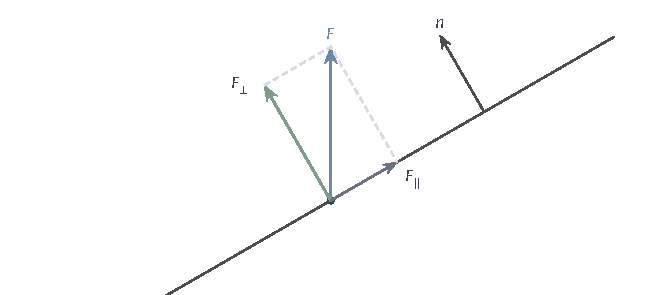
\includegraphics[width=112mm]{figures/01-mathematical-preliminaries-upper/00-shared/tikz/chapter3-concept-processes/normal-projection.pdf}
 \caption{黑斜线表示局部切平面的一个截面，$n$为所选单位法向。向量$F$分为$F_\perp=(F^\top n)n$与切向部分$F_\parallel$；通量使用有符号标量$F^\top n$乘面积，切向部分不贡献。将$n$改为$-n$时标量分量变号，但投影向量$F_\perp$不变，这与直接把场反向不同。}
 \label{fig:analysis-process-normal-projection}
\end{figure}

\paragraph{可积性的要求}

通量只累计法向分量，因此在法向分量可测的前提下，其有限可积性的准确条件是
\[
 \iint_E
 \left|\bm F(\bm r(u,v))^\top(\bm r_u\times\bm r_v)\right|
 \,\mathrm du\,\mathrm dv<\infty.
\]
一个更容易验证的充分条件是$\int_S\lVert\bm F\rVert_2\,\mathrm dS<\infty$：
因为$\lVert\bm n\rVert_2=1$，Cauchy--Schwarz不等式给出
$|\bm F^\top\bm n|\leq\lVert\bm F\rVert_2$，即法向分量不会超过场的大小。
连续向量场在本节的紧致有限分片曲面上有界，因而满足这一充分条件。

反过来，法向分量可积并不要求场的大小可积，因为切向分量再大也不进入通量。

\begin{example}[切向场大小不可积而通量为零]
\label{ex:analysis-tangential-field-zero-flux}
设$S=\{(x,y,0)^\top:x^2+y^2\leq1\}$是平面$z=0$上的单位圆盘，用参数$\bm r(x,y)=(x,y,0)^\top$，则$J_S=1$；取向上法向$\bm n=(0,0,1)^\top$。
令$\bm F(\bm x)=(\lVert\bm x\rVert_2^{-2},0,0)^\top$，原点处任取一值。
由极坐标换元（示例~\ref{ex:analysis-polar-coordinate-jacobian}），
\[
 \int_S\lVert\bm F\rVert_2\,\mathrm dS
 =\int_0^{2\pi}\int_0^1r^{-2}\cdot r\,\mathrm dr\,\mathrm d\theta
 =+\infty,
\]
所以场的大小不可积。
但$\bm F$平行于圆盘，$\bm F^\top\bm n=0$处处成立，法向分量可积，通量为$0$。
\end{example}

这个场的第一个分量在圆盘上不可积，通量却有定义。
所以不能把法向分量可积与向量场各分量都可积视为同一个条件。

\subsubsection{积分的性质}

以下运算都在同一曲面、同一法向约定下进行，并假定各法向分量可积。
它们大多可归结为标量函数$\bm F^\top\bm n$的面积积分，直接沿用第一类积分的性质；与方向有关的法向反转和重参数化则需要单独说明。

\paragraph{加法}

向量场相加以后，其法向分量也相加，因此
\[
 \begin{aligned}
 \int_S(\bm F+\bm G)^\top\bm n\,\mathrm dS
 &=\int_S\bm F^\top\bm n\,\mathrm dS\\
 &\quad{}+\int_S\bm G^\top\bm n\,\mathrm dS.
 \end{aligned}
\]
绝对可积性由两项法向分量的绝对值之和控制，积分等式来自标量面积积分的加法性质。
物理上，两股水流叠加后穿过网的水量，等于两股水流分别穿过的水量之和。

\paragraph{减法}

向量场相减以后，其法向分量也相减，因此
\[
 \begin{aligned}
 \int_S(\bm F-\bm G)^\top\bm n\,\mathrm dS
 &=\int_S\bm F^\top\bm n\,\mathrm dS\\
 &\quad{}-\int_S\bm G^\top\bm n\,\mathrm dS.
 \end{aligned}
\]
两项法向分量绝对可积时，它们的差仍绝对可积，积分等式来自标量面积积分的减法性质。

\paragraph{数乘}

对实数$c$，由$(c\bm F)^\top\bm n=c(\bm F^\top\bm n)$，常数可以提出积分号：
\[
 \int_S(c\bm F)^\top\bm n\,\mathrm dS
 =c\int_S\bm F^\top\bm n\,\mathrm dS.
\]
这里缩放的是场，曲面的法向约定保持固定：流速加倍，穿过的水量也加倍。

\paragraph{曲面分割的可加性}

将$S$分为内部不重叠的有限片$S_1,\ldots,S_N$，并在每片采用原定向的限制，则
\[
 \int_S\bm F^\top\bm n\,\mathrm dS
 =\sum_{j=1}^N\int_{S_j}\bm F^\top\bm n\,\mathrm dS.
\]
零面积接缝不贡献积分。
关键在于每片沿用原来的法向：若某片单独反转法向，这一片计入的是反方向的穿越量，加起来就不再是整张曲面的通量。

\paragraph{法向反转}

在场和曲面不变时，把$\bm n$换成$-\bm n$会使通量变号：
\[
 \int_S\bm F^\top(-\bm n)\,\mathrm dS
 =-\int_S\bm F^\top\bm n\,\mathrm dS.
\]
水流本身没有变，变的只是计数方向：例如原法向朝上时，从下往上的穿越原来记为正，现在记为负。
这与第一类积分不同，后者不使用法向，换定向不改变结果。

\paragraph{重参数化}

更换参数时，所选的几何法向保持不变。
由定理~\ref{thm:analysis-surface-reparameterization}，新参数的叉积等于原叉积乘$\det\bm J_T$，
而二维换元公式使用的是$|\det\bm J_T|$。若$\det\bm J_T>0$，两者相同，式~\eqref{eq:analysis-surface-flux}右端不变；
若$\det\bm J_T<0$，例如交换两个参数，新叉积指向相反一侧，按定义中“方向相反时乘$-1$”的约定校正后，结果仍不变。
因此在固定曲面定向并完成这一校正后，通量只依赖曲面、定向和场，与参数选择无关。

\subsubsection{积分的计算}

计算通量分三步：先确定要用哪一侧的法向，再选一个叉积指向该侧的参数化（若指向相反，就在结果前加负号），最后在参数域上累计$\bm F$与有向面积元的内积。

对于图像曲面$z=\psi(x,y)$，第一类积分的计算中已经求出叉积
\[
 \bm r_x\times\bm r_y=(-\psi_x,-\psi_y,1)^\top,
\]
它的第三分量为正，指向上方。
因此取向上法向时，对$\bm F=(P,Q,R)^\top$有
\[
 \int_S\bm F^\top\bm n\,\mathrm dS
 =\iint_D(-P\psi_x-Q\psi_y+R)(x,y,\psi(x,y))\,\mathrm dx\,\mathrm dy.
\]
取向下法向则在右侧加负号。这一式直接使用有向面积元，叉积的长度已经与单位法向的分母抵消，不能再额外乘一次$\sqrt{1+\psi_x^2+\psi_y^2}$。

斜平面片是$\psi(x,y)=x+y$在单位正方形上的图像，可以用它核对通量与投影面积的关系。

\begin{example}[竖直单位场穿过斜平面片]
\label{ex:analysis-tilted-plane-flux}
取斜平面片$\bm r(u,v)=(u,v,u+v)^\top$、$E=[0,1]^2$和向上单位法向$(-1,-1,1)^\top/\sqrt3$。
对竖直单位场$\bm F=(0,0,1)^\top$，场与参数叉积$(-1,-1,1)^\top$的内积为$1$，故
\[
 \int_S\bm F^\top\bm n\,\mathrm dS
 =\int_0^1\int_0^1 1\,\mathrm du\,\mathrm dv=1.
\]
用面积测度分开看：这块面的面积为$\sqrt3$（示例~\ref{ex:analysis-tilted-plane-area}），场的法向分量为$\bm F^\top\bm n=1/\sqrt3$，两者相乘为$1$，恰好等于它在$xy$平面上的投影面积。
\end{example}

同样地，平面$z=ax+by+c$在单位圆盘$D$上方的部分对该场的向上通量为$\iint_D1\,\mathrm dx\,\mathrm dy=\pi$，
等于水平投影面积；它的实际面积则为$\pi\sqrt{1+a^2+b^2}$。
这与示例~\ref{ex:analysis-tilted-square-flux}中倾斜屋顶接雨的结果一致：竖直的流只“看见”曲面的水平投影。

对半径为$R$的球面，讨论单位法向量时已算出$(\varphi,\theta)$次序的参数叉积为$R\sin\varphi\,\bm r$，它在参数域内部指向外侧。
下面三个例子都取外法向，依次计算径向场、点源场和恒定场的通量。

\begin{example}[径向场穿过球面]
\label{ex:analysis-radial-field-sphere-flux}
令$\bm F(\bm x)=\bm x/R$。在球面上$\bm F$恰等于外单位法向，$\bm F^\top\bm n=1$，由示例~\ref{ex:analysis-sphere-area}，
\[
 \int_S\bm F^\top\bm n\,\mathrm dS
 =\int_S1\,\mathrm dS=4\pi R^2.
\]
取内法向时通量为$-4\pi R^2$。
\end{example}

这次外向通量与面积相等，是因为法向分量处处为$1$。
一般情形下$|\bm F^\top\bm n|\leq\lVert\bm F\rVert_2$，通量的绝对值不超过场的大小对面积的积分；场的方向偏离法向时，只有法向分量计入通量。

接下来的两个例子形成对比：一个场由原点处的点源发出，另一个场在空间中处处相同。

\begin{example}[点源场的通量与半径无关]
\label{ex:analysis-point-source-sphere-flux}
令$\bm F(\bm x)=\bm x/\lVert\bm x\rVert_2^3$（$\bm x\neq\bm0$），$S$是以原点为中心、半径为$R$的球面，外法向为$\bm n=\bm x/R$。
$\bm F$在不含原点的球面上连续，因而法向分量可积。
在$S$上$\lVert\bm x\rVert_2=R$，故
\[
 \bm F^\top\bm n=\frac{\bm x^\top\bm x}{R^3\cdot R}=\frac1{R^2},
\]
外向通量为$(1/R^2)\cdot4\pi R^2=4\pi$。
\end{example}

球面越大，场越弱，但面积增大的倍数恰好抵消场的减弱，所以通量不随$R$改变：
以点源为中心的球面无论多大，测得的点源单位时间放出的总量都一样。

\begin{example}[恒定场穿过球面的净通量为零]
\label{ex:analysis-constant-field-sphere-flux}
令$\bm F=(0,0,1)^\top$。由$\bm r_\varphi\times\bm r_\theta=R\sin\varphi\,\bm r$，被积函数为
$\bm F^\top(\bm r_\varphi\times\bm r_\theta)=R\sin\varphi\cdot R\cos\varphi=R^2\sin\varphi\cos\varphi$，于是
\[
 \int_S\bm F^\top\bm n\,\mathrm dS
 =\int_0^{2\pi}\int_0^\pi R^2\sin\varphi\cos\varphi\,\mathrm d\varphi\,\mathrm d\theta=0.
\]
分开计算，上半球面$0\leq\varphi\leq\pi/2$的外向通量为
\[
 2\pi R^2\int_0^{\pi/2}\sin\varphi\cos\varphi\,\mathrm d\varphi=\pi R^2,
\]
下半球面$\pi/2\leq\varphi\leq\pi$的外向通量为$-\pi R^2$。
\end{example}

在恒定场中，水从下半球面流入球内，又从上半球面等量流出，球内既不产生也不吸收水，所以闭曲面的净通量为零。
包围点源的球面则有正的净通量。
可见闭曲面的净通量反映它所围区域内部的源与汇；
第~\ref{sec:multivariable-boundary-relations}节将用区域内部的散度累计来计算闭曲面的通量，并核对这里的几个结果。

\FloatBarrier

\section{三类积分之间的关系}
\label{sec:multivariable-boundary-relations}

一元微积分基本定理说，若$f$在$[a,b]$上连续可微，则导数$f'$在区间上的积分等于$f(b)-f(a)$：区间内部各点的变化率累计起来，只剩下两个端点上的函数值。
区间的边界就是这两个端点，所以$f(b)-f(a)$也可以读成带符号的边界求和：右端点记正号，左端点记负号。
路径积分基本定理（式~\eqref{eq:analysis-line-integral-gradient}）把同样的关系搬到路径上：梯度场沿路径的积分，等于势函数在终点与起点的值之差。

本节把这种“内部导数的累计等于边界上的累计”的关系推广到平面区域、空间区域和曲面。
三种推广共用一个思路。先把对象切成许多小块；在每个小块上，某个导数乘小块的大小，近似等于向量场沿小块边界的累计。
相邻两块的公共边界被两块各算一次，两次的方向相反，相加后抵消，最后只剩下整个对象的外边界。
按边界的类型，本节回答三个问题：平面区域上的积分何时等于边界路径积分，这是Green公式；空间区域上的积分何时等于边界曲面积分，这是Gauss公式；曲面上的积分何时等于曲面边界的路径积分，这是Stokes公式。

这些公式中的被积对象不能互换。沿边界的环流累计向量场的切向分量，对应的内部量是旋度，它衡量场绕一点旋转的强度；
穿过边界的通量累计向量场的法向分量，对应的内部量是散度，它衡量场从一点向外发散的强度。

为此，本节先定义这两种导数以及Laplace算子，并说明它们的物理含义；再规定边界的方向；最后给出各公式的条件、推导和例子。
所有区域积分以及路径、曲面的参数积分均采用勒贝格积分。经典公式的组织参考向量微积分教材\scite{math-openstax-calculus3}。

\subsection{积分公式中的微分算子}

定义~\ref{def:multivariable-gradient}把标量函数的各个一阶偏导数排成梯度。现在考虑开集$U$上的向量场$\bm F$，不妨把它想成流体的速度场：$\bm F(\bm x)$是流体在位置$\bm x$处的速度。
对这样的场，有两个自然的局部问题：在一点附近，流体是净流出还是净流入；流体是否绕这一点打转。
两个问题的答案都由$\bm F$各分量的一阶偏导数决定，但用到的偏导数组合不同。
回答前一个问题的是散度，回答后一个问题的是旋度，二者都以向量场为输入；随后的Laplace算子以标量函数为输入，比较函数在一点的值与周围平均值的差别。

\subsubsection{散度}

\paragraph{小立方体的净流出}

设$\bm F=(F_1,F_2,F_3)^\top$是三维流体的速度场。第~\ref{sec:analysis-surface-integration}节定义的通量只取速度的法向分量，原因如下。
在很短的时间$\Delta t$内，穿过面积为$\Delta S$、单位法向为$\bm n$的一小片曲面的流体，占据一个底面积为$\Delta S$、高约为$(\bm F^\top\bm n)\Delta t$的斜柱；所以单位时间穿过这一小片的流体体积约为$(\bm F^\top\bm n)\Delta S$，速度的切向分量只让流体沿曲面滑动，不贡献穿过量。
现在以点$\bm a$为中心取边长为$h$的小立方体，各面与坐标平面平行，估计单位时间从它流出的净体积。

先看与$x$轴垂直的两张面。右面$x=a_1+h/2$的外法向是$\bm e_1$，场在这张面上的法向分量是$F_1$；用面中心的值代表整张面，流出量约为$F_1(\bm a+\tfrac h2\bm e_1)h^2$。
左面$x=a_1-h/2$的外法向是$-\bm e_1$，流出量约为$-F_1(\bm a-\tfrac h2\bm e_1)h^2$；$F_1>0$时这个量为负，表示沿$x$正方向的流动在左面是流入。两面合计为
\[
 \Bigl[F_1\bigl(\bm a+\tfrac h2\bm e_1\bigr)-F_1\bigl(\bm a-\tfrac h2\bm e_1\bigr)\Bigr]h^2
 \approx \partial_1F_1(\bm a)\,h\cdot h^2,
\]
这里用偏导数乘距离$h$近似了$F_1$在两张面中心之间的差。
若$F_1$沿$x$方向增大，从右面流出的比从左面流入的多，这对面贡献正的净流出；若$F_1$沿$x$方向不变，流入与流出恰好相等。

另外两对面同样分别给出约$\partial_2F_2(\bm a)h^3$和$\partial_3F_3(\bm a)h^3$。六张面合计后除以体积$h^3$，得到
\[
 \frac{\text{小立方体的净流出}}{\text{小立方体的体积}}
 \approx\partial_1F_1(\bm a)+\partial_2F_2(\bm a)+\partial_3F_3(\bm a).
\]
这里只做了一阶近似。在Gauss公式（定理~\ref{thm:analysis-divergence-theorem}）之后将证明，当$\bm F$连续可微且$h\to0$时，左侧确实收敛到右侧。右侧的偏导数之和称为散度。
\begin{definition}[散度]
\label{def:multivariable-divergence}
设$U\subseteq\mathbb R^d$为开集，$\bm F=(F_1,\ldots,F_d)^\top:U\to\mathbb R^d$的各分量一阶偏导数存在。
$\bm F$的\term{散度}（divergence）是标量函数
\[
 \operatorname{div}\bm F
 =\nabla\mathbin{\cdot}\bm F
 =\sum_{j=1}^d\partial_jF_j.
\]
\end{definition}

\paragraph{源的强度}

按小立方体上的推导，散度是单位体积的净流出率，可以理解为一点处“源”的强度。
$\operatorname{div}\bm F(\bm a)>0$表示$\bm a$附近像有一个源，流体在这里产生并向外流走；$\operatorname{div}\bm F(\bm a)<0$表示这里像一个汇，流入的多于流出的；散度为零表示流入与流出平衡。
若流体不可压缩，内部又没有注入或抽出流体的源和汇，则每个小体积的流入量都等于流出量，速度场的散度处处为零。

下面三个场分别对应均匀膨胀、绕轴转动和整体平移，可以用来检验这一解释。
\begin{example}[径向场、旋转场与常场的散度]
三维径向场$\bm F(x,y,z)=(x,y,z)^\top$满足$\partial_xF_1=\partial_yF_2=\partial_zF_3=1$，所以$\operatorname{div}\bm F=1+1+1=3$：流体从各处均匀地向外膨胀，每单位体积每单位时间多出$3$个单位体积的流体。

旋转场$\bm G(x,y,z)=(-y,x,0)^\top$的第一分量不含$x$，第二分量不含$y$，第三分量为零，所以$\operatorname{div}\bm G=0+0+0=0$：流体绕$z$轴转动，任何小立方体流入多少就流出多少。

常场$\bm H=(1,0,0)^\top$的各分量都是常数，散度同样为$0$：流体整体平移，每个小立方体从左面流入的量都从右面流出。
\end{example}
旋转场和常场都不是零场，散度却都为零。可见散度为零只表示局部净流出率为零，并不表示向量场为零。

二维场$(P,Q)^\top$的散度相应为$P_x+Q_y$，它是小正方形四条边上的净流出除以面积所得的极限；定理~\ref{thm:multivariable-planar-flux}的平面通量公式使用这一标量函数。

\subsubsection{旋度}

\paragraph{小正方形上的环流}

净流出不能描述绕一点旋转的运动。旋转场$\bm G=(-y,x,0)^\top$的散度为零，但在水平平面内沿以$z$轴上一点为圆心的圆周逆时针走一圈，场始终与行进方向相同，环流不为零。
为了度量一点附近的旋转，先在平面上计算小正方形边界的环流。设平面场为$(P,Q)^\top$，以$\bm a$为中心取边长为$h$的正方形，沿逆时针方向走一圈。

下边从左向右，切向分量是$P$，贡献约$P(\bm a-\tfrac h2\bm e_2)h$；上边从右向左，贡献约$-P(\bm a+\tfrac h2\bm e_2)h$；两者合计约$-\partial_yP(\bm a)h^2$。
右边从下向上，贡献约$Q(\bm a+\tfrac h2\bm e_1)h$；左边从上向下，贡献约$-Q(\bm a-\tfrac h2\bm e_1)h$；两者合计约$\partial_xQ(\bm a)h^2$。四边相加后除以面积$h^2$，得到
\[
 \frac{\text{小正方形边界的逆时针环流}}{\text{小正方形的面积}}
 \approx\partial_xQ(\bm a)-\partial_yP(\bm a).
\]
两项的符号可以这样理解。若$Q$沿$x$方向增大，右边向上的流速比左边大，这一对边推动逆时针转动；若$P$沿$y$方向增大，上边向右的流速比下边大，这一对边推动顺时针转动，所以$\partial_yP$带负号。

在三维空间中，小正方形可以放在分别垂直于三个坐标轴的平面里，行进方向都取从相应坐标轴正方向看的逆时针。
垂直于$z$轴时，平面坐标是$(x,y)$，$(F_1,F_2)$相当于$(P,Q)$，同样的计算给出$\partial_xF_2-\partial_yF_1$；
垂直于$x$轴时，平面坐标的次序是$(y,z)$，$(F_2,F_3)$相当于$(P,Q)$，得到$\partial_yF_3-\partial_zF_2$；
垂直于$y$轴时，平面坐标的次序是$(z,x)$，$(F_3,F_1)$相当于$(P,Q)$，得到$\partial_zF_1-\partial_xF_3$。
这样选取坐标次序，是因为$\bm e_2\times\bm e_3=\bm e_1$、$\bm e_3\times\bm e_1=\bm e_2$：从坐标轴正方向看，第一个平面坐标轴逆时针转过直角得到第二个。
把这三个环流率按$x,y,z$轴的次序排成一个向量，就得到旋度。
\begin{definition}[旋度]
\label{def:multivariable-curl}
设$U\subseteq\mathbb R^3$为开集，$\bm F=(F_1,F_2,F_3)^\top:U\to\mathbb R^3$的各分量一阶偏导数存在。
$\bm F$的\term{旋度}（curl）是向量场
\[
 \operatorname{curl}\bm F=\nabla\times\bm F
 =\begin{pmatrix}
   \partial_yF_3-\partial_zF_2\\
   \partial_zF_1-\partial_xF_3\\
   \partial_xF_2-\partial_yF_1
  \end{pmatrix}.
\]
\end{definition}

\paragraph{旋转的轴与强度}

坐标平面上的三个计算可以推广到任意方向。设$\bm F$连续可微，$\bm n$是单位向量；在过点$\bm a$且垂直于$\bm n$的平面内，取以$\bm a$为中心的小正方形或小圆周，从$\bm n$的箭头一侧看按逆时针行进。
尺寸趋于零时，环流除以所围面积的极限等于$(\operatorname{curl}\bm F)(\bm a)^\top\bm n$。$\bm n$为坐标轴方向时，这就是上面的计算；一般方向的证明放在Stokes公式之后。

由Cauchy--Schwarz不等式，$(\operatorname{curl}\bm F)^\top\bm n\leq\lVert\operatorname{curl}\bm F\rVert_2$；旋度不为零时，等号当且仅当$\bm n$与旋度同向时成立。
所以旋度的方向是局部旋转最强的转轴，其长度是旋转的强度；转向由右手定则确定：右手大拇指沿旋度方向，其余四指弯曲的方向就是转向。

一个物理图像是放进流水中的小桨轮。让桨轮的转轴沿$\bm n$，水流沿轮缘推动各个叶片；桨轮是否转动、往哪边转，取决于沿轮缘的环流，也就是$(\operatorname{curl}\bm F)^\top\bm n$的符号；转轴与旋度平行时转得最快。
这一图像帮助理解定义，但不代替上面的计算。

先用整体转动和径向膨胀检验这一图像。
\begin{example}[刚体旋转与径向膨胀的旋度]
\label{ex:analysis-rigid-rotation-curl}
整体以角速度$\omega$绕$z$轴旋转的流体，速度场为$\bm F=\omega(-y,x,0)^\top$。代入定义，前两个分量$\partial_yF_3-\partial_zF_2$与$\partial_zF_1-\partial_xF_3$都为零，第三个分量为$\partial_x(\omega x)-\partial_y(-\omega y)=2\omega$，所以$\nabla\times\bm F=(0,0,2\omega)^\top$。
特别地，$\omega=1/2$时$\bm F=(-y/2,x/2,0)^\top$，旋度为$(0,0,1)^\top$。

径向场$(x,y,z)^\top$的第$i$个分量只依赖第$i$个坐标，旋度定义中的每个交叉偏导数都为零，所以旋度为零：流体只向外膨胀而不打转。
\end{example}
刚体旋转的旋度沿转轴，长度是角速度的两倍，与桨轮图像一致。不过，旋度与流线是否弯曲并不是一回事，下面两个场从相反的方向说明这一点。
\begin{example}[剪切流与涡旋场]
剪切流$\bm F=(y,0,0)^\top$的流线都是水平直线。它的偏导数中只有$\partial_yF_1=1$不为零，所以$\nabla\times\bm F=(0,0,-1)^\top$。
物理上，上方的水比下方的水向右流得快，桨轮的上缘被推得更多，从$z$轴正方向看桨轮顺时针转动，与第三分量为负一致。

再看平面上沿同心圆流动的场。设流体在每个以原点为圆心的圆周上逆时针流动，半径为$r$的圆周上速率为$s(r)>0$，其中$s$可微，即
\[
 (P,Q)^\top=g(r)\,(-y,x)^\top,\qquad g(r)=\frac{s(r)}r,\quad r=\sqrt{x^2+y^2}>0.
\]
由$\partial_xr=x/r$、$\partial_yr=y/r$，有$Q_x=g(r)+g'(r)x^2/r$、$P_y=-g(r)-g'(r)y^2/r$，所以
\[
 Q_x-P_y=2g(r)+rg'(r)=\frac{s(r)}r+s'(r).
\]
第一项$s(r)/r$来自流线的弯曲，第二项$s'(r)$来自不同半径上流速的差别。刚体旋转$s(r)=\omega r$时两项都等于$\omega$，合计$2\omega$，与前例一致。
第~\ref{sec:multivariable-potential-path-independence}节穿孔平面上的涡旋场$(-y,x)^\top/(x^2+y^2)$对应$s(r)=1/r$，两项分别为$1/r^2$与$-1/r^2$，所以在原点以外$Q_x-P_y=0$。
\end{example}
剪切流的流线是直线，旋度却不为零；涡旋场的流线弯曲，在原点以外旋度却为零。后者的原因是：流线弯曲带来的逆时针倾向，恰好被外侧流速较慢带来的顺时针倾向抵消，所以放在原点以外的小桨轮不转。

对二维场$(P,Q)^\top$，平面内需要的是标量$Q_x-P_y$。
把二维场补上为零的第三分量，写成三维场$(P,Q,0)^\top$后，这一标量正是旋度的第三分量，也就是旋度在向上法向$\bm e_3$上的分量。
符号$\nabla\mathbin\cdot$和$\nabla\times$表示这里定义的偏导数组合，不是两个普通数值向量的内积或叉积。


图~\ref{fig:analysis-process-divergence-circulation-fields}在同一个单位圆周上分别观察净流出与切向环流，比较两种微分算子所记录的信息。
\begin{figure*}[!htbp]
 \centering
 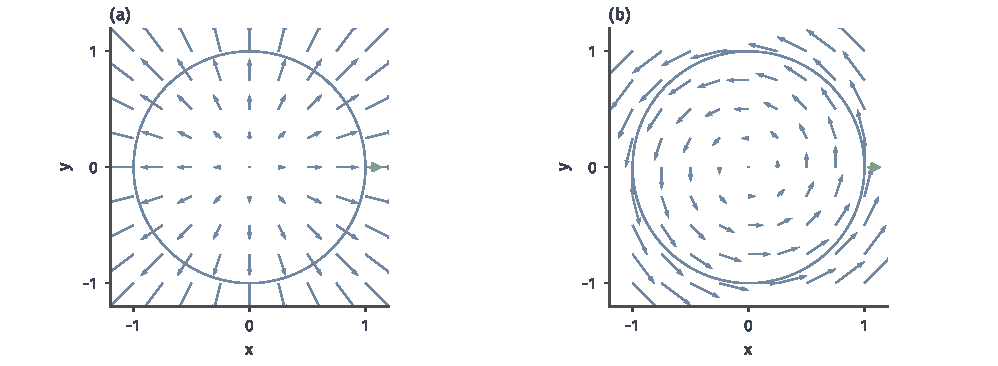
\includegraphics[width=169.0mm]{figures/01-mathematical-preliminaries-upper/00-shared/matplotlib/chapter3-concept-processes/divergence-circulation-fields.pdf}
 \caption{(a) 径向场$(x,y)^\top$的二维散度为$2$、旋转率$Q_x-P_y=0$，圆周外向通量为$2\pi$、环流为零。(b) 旋转场$(-y,x)^\top$的散度为零、旋转率为$2$，通量为零、环流为$2\pi$。绿箭头仅标记外法向；蓝色场箭头按相同常数缩放。零散度不等于零场，也不等于零环流。}
 \label{fig:analysis-process-divergence-circulation-fields}
\end{figure*}

\subsubsection{Laplace算子}

标量函数的梯度是向量场，因此可以对它继续取散度，把各坐标方向的二阶变化相加。
这一复合运算出现在多元分部积分中，也出现在描述热传导和扩散的方程中；它的输入与输出都是标量函数。
\begin{definition}[Laplace算子]
\label{def:multivariable-laplacian}
对开集$U\subseteq\mathbb R^d$上的二阶连续可微标量函数$v$，定义\term{Laplace算子}（Laplacian）为
\[
 \Delta v=\operatorname{div}(\nabla v)
 =\sum_{j=1}^d\partial_j^2v.
\]
\end{definition}
梯度把标量函数变为向量场，散度再把向量场变为标量函数，所以$\Delta v$仍是标量函数；它与输入、输出都是向量场的旋度属于不同类型的运算。

\paragraph{与邻域平均值的差}

一元情形中，$v''(a)>0$表示函数在$a$附近向上弯，$v(a)$低于两侧邻点的平均值。多元情形可以做同样的比较。
在$\bm a$的每个坐标方向上各取前后两个邻点$\bm a\pm h\bm e_j$，沿该坐标作二阶Taylor展开：
\[
 v(\bm a+h\bm e_j)+v(\bm a-h\bm e_j)-2v(\bm a)=h^2\partial_j^2v(\bm a)+o(h^2),
\]
一阶项$\pm h\partial_jv(\bm a)$在两点相加时抵消。对$j=1,\ldots,d$求和，再除以邻点个数$2d$，得到
\[
 \frac1{2d}\sum_{j=1}^d\bigl[v(\bm a+h\bm e_j)+v(\bm a-h\bm e_j)\bigr]-v(\bm a)
 =\frac{h^2}{2d}\Delta v(\bm a)+o(h^2).
\]
因此，$h$足够小时，$\Delta v(\bm a)>0$表示$v(\bm a)$低于周围邻点的平均值，$\Delta v(\bm a)<0$表示高于平均值；$\Delta v(\bm a)=0$表示二者之差是$o(h^2)$，在这一精度下相等。

下面用两个二次函数直接比较邻点平均值与中心值。
\begin{example}[二次函数的邻点平均]
取$v(x,y,z)=x^2+y^2+z^2$，则$\Delta v=2+2+2=6$。在原点，$v(\bm0)=0$；六个邻点$\pm h\bm e_j$上的值都是$h^2$，所以邻点平均值比中心值高$h^2$，恰等于$\frac{h^2}{2d}\Delta v=\frac{h^2}6\cdot6$。二次函数的Taylor展开没有余项，等式精确成立。

再取$v(x,y)=x^2-y^2$，则$\Delta v=2-2=0$。原点的四个邻点$(\pm h,0)$与$(0,\pm h)$上的取值为$h^2,h^2,-h^2,-h^2$，平均值恰为$0=v(\bm0)$。
\end{example}
第二个函数在$x$方向向上弯、在$y$方向向下弯，两种弯曲正好抵消。Laplace算子记录的是各坐标方向弯曲的总和，不能据此判断每个方向各自的弯曲。

\paragraph{热传导中的含义}

设$u(t,\bm x)$是时刻$t$物体内位置$\bm x$处的温度，它对$\bm x$二阶连续可微。热量从高温处流向低温处，Fourier热传导定律把单位时间穿过单位面积的热流写成$\bm q=-k\nabla u$，其中常数$k>0$为导热系数，$\nabla$只作用于空间变量$\bm x$\scite{math-openstax-calculus3}。
由散度的含义，单位体积的热量净流出率为$\operatorname{div}\bm q=-k\Delta u$。没有热源时，单位体积内热量的增加率等于净流入率$-\operatorname{div}\bm q=k\Delta u$；再除以单位体积的热容$c>0$，得到温度的变化率
\[
 \partial_tu=\frac kc\,\Delta u,
\]
这就是热传导方程。

这个方程说明温度怎样随时间变化。比周围平均更冷的点满足$\Delta u>0$，会从周围吸收热量而升温；比周围平均更热的点满足$\Delta u<0$，会降温；温度分布因而逐渐被抹平。
温度不再随时间变化时，处处有$\Delta u=0$；按邻域平均值的公式，每点的温度在上述精度下等于周围的平均。这里的Fourier定律是物理模型，本节只用它说明$\Delta$的含义。

\subsection{边界的定向}

将一个区域分成相邻小块时，公共边或公共面不属于原区域的外边界。
要使这些内部贡献相消，各小块必须采用相容的方向；同时，每个小块的方向还要与小块上局部计算所用的方向一致：环流按逆时针计算，通量按外法向计算。
下面依次规定平面区域边界的行进方向、区域边界的外法向，以及定向曲面边界的行进方向。

\subsubsection{平面区域的正向边界}

平面区域的边界是路径，所以先规定沿边界行进的方向。本节考虑的平面区域，边界由若干条简单闭曲线组成；简单闭曲线指除首尾相合外不自交的闭曲线。
对有界平面区域，取边界方向使沿曲线前进时区域总在左侧，称为正向边界。
沿单位圆逆时针行走，单位圆盘始终在左手边，所以圆盘的正向边界是逆时针方向。

有孔洞时，外边界仍是逆时针；围绕孔洞的内边界要使区域而非孔洞留在左侧，因而是顺时针。
例如圆环$1<x^2+y^2<4$的外圈$r=2$逆时针、内圈$r=1$顺时针，两圈边界方向相反。
这个约定与小块相消的要求一致：把圆环切成许多小块，每块都按逆时针走边界，内部公共边相互抵消后，剩在孔洞边上的那些边恰好被顺时针走过。

边界由多段光滑弧组成时，按这一方向逐段相接，转角处不另加积分项。
一般地，相邻平面小块各自采用正向边界时，共同边被沿相反方向走过，两个有向路径积分恰好抵消。

\subsubsection{区域边界的外法向}

通量需要的是法向，而不是边界的行进方向。空间区域的外单位法向从内部指向外部；有孔洞时，孔洞边界的外法向指向孔洞。
例如球壳$1<\lVert\bm x\rVert_2<2$在外球面上的外法向背离原点，在内球面上的外法向指向原点。
相邻子区域的公共面上，两侧子区域的外法向相反，所以内部通量相消。

平面区域边界上的外单位法向按同样方式规定，只是通量沿边界按弧长累计。
外法向与正向边界的单位切向量$\bm\tau=(\tau_1,\tau_2)^\top$有固定关系：区域在行进方向的左侧，外侧就在右侧，所以把$\bm\tau$顺时针转过直角就得到外法向$\bm n=(\tau_2,-\tau_1)^\top$。
例如在单位圆的点$(1,0)$处，逆时针的切向量是$(0,1)^\top$，按此公式得到$(1,0)^\top$，确实指向圆外。

\subsubsection{定向曲面边界的诱导方向}

曲面取定单位法向$\bm n$后，其边界路径的方向不能再任意选择。
边界的正向按右手约定确定：右手大拇指朝法向，其余手指弯曲的方向为正向，称为由法向诱导的方向，简称诱导方向。
等价地，沿边界前进并把头朝向法向时，曲面留在左侧。面朝前进方向$\bm f$、头顶朝$\bm u$站立时，左手方向是$\bm u\times\bm f$；用这个叉积可以核对具体例子。

下面用这个叉积核对两张以单位圆为边界的曲面，后面检验Stokes公式时会用到它们。
\begin{example}[向上圆盘与外向上半球面的诱导方向]
\label{ex:analysis-hemisphere-induced-orientation}
对取向上法向$\bm e_3$的单位圆盘，在边界点$(1,0,0)$处取前进方向$\bm f=\bm e_2$，左手方向为$\bm e_3\times\bm e_2=-\bm e_1$，指向圆盘内部。所以诱导方向是从上方看逆时针。

对取外法向的上半单位球面，赤道上的点$(1,0,0)$处外法向是$\bm e_1$。同样取前进方向$\bm f=\bm e_2$，左手方向为$\bm e_1\times\bm e_2=\bm e_3$，正指向半球面所在的上方。所以它的诱导方向也是从上方看逆时针，与向上圆盘的边界方向相同。
\end{example}
两张曲面在边界点处的法向不同，曲面伸出的方向也不同；但二者都满足“头朝法向时曲面在左侧”，所以诱导出同一个边界方向。

若翻转曲面法向，边界的诱导方向也随之翻转。分片曲面的定向相容，指相邻曲面片在公共边上诱导出相反的行进方向。
这时公共边上的路径积分相消，只留下整张曲面的真正边界。


图~\ref{fig:analysis-process-boundary-orientation-cancellation}把相容方向的作用画出来：只有内部公共边相消，才会只剩下整个对象的外边界。
\begin{figure}[!htbp]
 \centering
 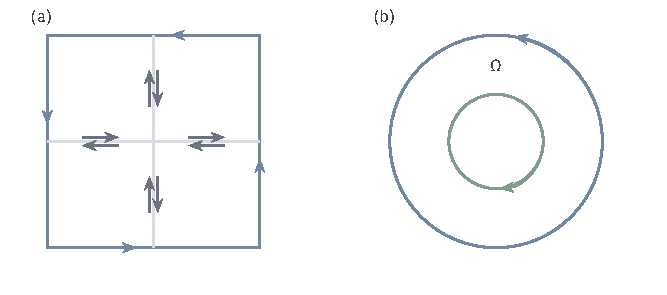
\includegraphics[width=112mm]{figures/01-mathematical-preliminaries-upper/00-shared/tikz/chapter3-concept-processes/boundary-orientation-cancellation.pdf}
 \caption{(a) 四个小正方形各取逆时针正向，共同边被沿相反方向走过；灰箭头略错开以便辨认，实际是同一条边。相加后只留下蓝色外边界。(b) 圆环的外边界逆时针、孔洞边界顺时针，沿任一边界前进时区域均在左侧。曲面拼片时也按公共边相反方向保证Stokes边界项相消。}
 \label{fig:analysis-process-boundary-orientation-cancellation}
\end{figure}

\subsection{平面区域积分与边界路径积分}

在平面上，区域的边界是一维路径。对同一个二维向量场，可以沿边界累计切向分量，得到环流；也可以累计外法向分量，得到通量。
两种边界积分分别对应区域内部的$Q_x-P_y$和散度$P_x+Q_y$。

\subsubsection{Green公式的环流形式}

旋度一节在小正方形上算出：逆时针环流约等于$Q_x-P_y$乘正方形面积。
把区域$\Omega$划分成许多小正方形（靠近弯曲边界处是不规则的小块），对每块写出这一近似再相加。
相邻两块的公共边在两块中方向相反，贡献抵消，剩下的只有沿$\Omega$正向边界的环流；另一侧各块“$Q_x-P_y$乘面积”之和，则是区域积分的近似和。
Green公式说明，在适当条件下这一近似在加细后成为精确等式：区域内各处微小旋转的累计，等于沿边界走一圈的总环流。
\begin{theorem}[Green公式]
\label{thm:multivariable-green}
设$\Omega\subseteq\mathbb R^2$为有界开区域，边界由有限条分段$C^1$简单闭曲线组成，
且区域在每段光滑边界附近位于边界的一侧。边界取正向，即外边界逆时针、孔洞边界顺时针。
若二维向量场$\bm F=(P,Q)^\top$在$\overline\Omega$的开邻域内连续可微，则\term{Green公式}（Green's theorem）给出
\begin{equation}
 \oint_{\partial\Omega}P\,\mathrm dx+Q\,\mathrm dy
 =\iint_\Omega\left(\frac{\partial Q}{\partial x}-\frac{\partial P}{\partial y}\right)\,\mathrm dx\,\mathrm dy.
 \label{eq:multivariable-green}
\end{equation}
\end{theorem}
左侧是向量场的切向路径积分；右侧是标量函数$Q_x-P_y$的区域积分。
在矩形上，二者的等式可以直接由一元基本定理和Fubini定理推出。
\begin{proof}[矩形情形的证明]
取$\Omega=(a,b)\times(c,d)$，先写出左侧沿四条边的贡献。下边$(t,c)$、$a\leq t\leq b$从左向右，$\mathrm dy=0$，贡献$\int_a^bP(x,c)\,\mathrm dx$；
上边从$(b,d)$走到$(a,d)$，贡献$-\int_a^bP(x,d)\,\mathrm dx$；右边从下向上，贡献$\int_c^dQ(b,y)\,\mathrm dy$；左边从上向下，贡献$-\int_c^dQ(a,y)\,\mathrm dy$。
水平边上$\mathrm dy=0$，竖直边上$\mathrm dx=0$，所以$Q$只在竖直边出现，$P$只在水平边出现。

再看右侧。场在闭矩形附近连续可微，以下被积函数均可积。固定$x$，对$y$用一元基本定理得$\int_c^d\partial_yP(x,y)\,\mathrm dy=P(x,d)-P(x,c)$；再对$x$积分，并由Fubini定理换成区域积分。对$Q$则先固定$y$、对$x$积分。于是
\[
 \begin{aligned}
 -\iint_\Omega\partial_yP\,\mathrm dx\,\mathrm dy
 &=\int_a^b[P(x,c)-P(x,d)]\,\mathrm dx,\\
 \iint_\Omega\partial_xQ\,\mathrm dx\,\mathrm dy
 &=\int_c^d[Q(b,y)-Q(a,y)]\,\mathrm dy.
 \end{aligned}
\]
第一行恰是下边与上边的两项，第二行恰是右边与左边的两项。
四项合起来，正是沿下、右、上、左四条边逆时针行进得到的路径积分。
\end{proof}
有限个矩形拼接时，公共边上的积分因方向相反而抵消。
一般规则区域的证明还需处理区域分片及边界逼近误差，不能仅凭小矩形上的等式完成；这里引用一般形式，完整论证可参考向量微积分教材\scite{math-strang1991calculus}。

先用旋转场在单位圆盘上核对公式两侧，并观察边界方向的作用。
\begin{example}[旋转场在单位圆盘上的Green公式]
\label{ex:analysis-rotation-field-green-disk}
取$\bm F=(P,Q)^\top=(-y,x)^\top$，$\Omega$为单位圆盘。$\bm F$在整个平面上连续可微，定理条件满足。
右侧被积函数为$Q_x-P_y=1-(-1)=2$，区域积分为$2\cdot\pi=2\pi$。
左侧取逆时针边界$\gamma(t)=(\cos t,\sin t)^\top$，$0\leq t\leq2\pi$，则$\bm F(\gamma(t))^\top\gamma'(t)=\sin^2t+\cos^2t=1$，积分同样为$2\pi$。
若把圆周改为顺时针，左侧变为$-2\pi$，右侧仍为$2\pi$，等式不再成立。
\end{example}
区域积分不含方向信息，边界积分却随方向反转而变号；Green公式的符号由正向边界的约定决定。

Green公式也可以反过来使用：选一个满足$Q_x-P_y\equiv1$的场，右侧就是区域的面积，于是面积可以由边界环流算出。
\begin{example}[用边界计算面积]
\label{ex:analysis-green-area-formula}
设$\Omega$满足定理~\ref{thm:multivariable-green}的条件。取$P=-y/2$、$Q=x/2$，则$Q_x-P_y=1$，Green公式给出
\[
 \operatorname{area}(\Omega)=\frac12\oint_{\partial\Omega}x\,\mathrm dy-y\,\mathrm dx.
\]
对半轴为$\alpha,\beta>0$的椭圆区域，正向边界取$\gamma(t)=(\alpha\cos t,\beta\sin t)^\top$、$0\leq t\leq2\pi$。这时$\mathrm dx=-\alpha\sin t\,\mathrm dt$、$\mathrm dy=\beta\cos t\,\mathrm dt$，
\[
 x\,\mathrm dy-y\,\mathrm dx=(\alpha\beta\cos^2t+\alpha\beta\sin^2t)\,\mathrm dt=\alpha\beta\,\mathrm dt,
\]
所以面积为$\frac12\cdot2\pi\alpha\beta=\pi\alpha\beta$。
\end{example}
这个公式只需要沿边界走一圈、记录坐标与位移，就能得到所围面积；机械求积仪正是按这一原理工作的。

定理要求场在$\overline\Omega$的开邻域内连续可微。区域包含场的奇点时，这一条件不再满足，下面的例子说明它不能省略。
\begin{example}[有孔区域上的涡旋场]
\label{ex:analysis-annulus-vortex-green}
第~\ref{sec:multivariable-potential-path-independence}节的穿孔平面反例中，$\bm F=(-y,x)^\top/(x^2+y^2)$在原点以外满足$Q_x-P_y=0$，但沿单位圆逆时针一周的环流为$2\pi$。

取圆环$\Omega=\{1<x^2+y^2<4\}$。它的闭包不含原点，$\bm F$在$\overline\Omega$的一个开邻域内连续可微，Green公式适用，右侧为$0$。
左侧由两圈组成。外圈$r=2$逆时针，参数化为$(2\cos t,2\sin t)^\top$，此时$\bm F=(-\sin t,\cos t)^\top/2$，与速度$(-2\sin t,2\cos t)^\top$的内积为$1$，环流为$2\pi$；内圈$r=1$按正向取顺时针，环流为$-2\pi$。两者相加为零，与右侧一致。
\end{example}
外圈逆时针为$2\pi$、内圈顺时针为$-2\pi$，也就是说，两条圆周按同一逆时针方向走时环流都是$2\pi$。环流来自场在原点处的奇异，而不是来自圆环内部。
单位圆盘含有原点，$\bm F$在那里无定义，不满足Green公式的条件，所以不能由$Q_x-P_y=0$推出单位圆上的环流为零。

\subsubsection{Green公式的通量形式}

现在把平面向量场想成薄层流体的速度场，问单位时间有多少流体穿过区域边界流出。
每个小正方形的净流出约等于散度乘面积；相邻两块的公共边上外法向相反，一块的流出就是另一块的流入，相加后抵消。
因此可以预期：区域内部源强度的总和，等于穿过边界的净流出。

计算通量需要把场投影到外法向上。正向边界的有向位移是$\bm\tau\,\mathrm ds=(\mathrm dx,\mathrm dy)^\top$，而外法向由$\bm\tau$顺时针转过直角得到，因此
\[
 \bm n\,\mathrm ds=(\mathrm dy,-\mathrm dx)^\top.
\]
这一关系把法向通量写成切向路径积分，从而可以使用Green公式。
\begin{theorem}[平面区域的通量公式]
\label{thm:multivariable-planar-flux}
在与Green公式相同的区域条件下，若$\bm F=(F_1,F_2)^\top$在$\overline\Omega$的开邻域内连续可微，
$\bm n$是边界的外单位法向，则
\[
 \int_{\partial\Omega}\bm F^\top\bm n\,\mathrm ds
 =\iint_\Omega\operatorname{div}\bm F\,\mathrm dx\,\mathrm dy.
\]
\end{theorem}
\begin{proof}
利用外法向与正向边界的关系，$\bm F^\top\bm n\,\mathrm ds=F_1\,\mathrm dy-F_2\,\mathrm dx$，所以左侧等于
$\oint_{\partial\Omega}(-F_2)\,\mathrm dx+F_1\,\mathrm dy$。
在Green公式中取$(P,Q)=(-F_2,F_1)$，右侧被积函数为$Q_x-P_y=\partial_xF_1+\partial_yF_2=\operatorname{div}\bm F$。
\end{proof}
这也是二维的散度公式。它与环流形式使用相同的区域条件，但累计的边界分量和内部导数不同。

下面在单位圆盘上比较两个场的通量：一个从各处均匀发散，一个只绕原点打转。
\begin{example}[单位圆盘上径向场与旋转场的通量]
取$\bm F(x,y)=(x,y)^\top$，$\Omega$为单位圆盘。散度为$1+1=2$，区域积分为$2\pi$。
边界参数化为$\gamma(t)=(\cos t,\sin t)^\top$，$0\leq t\leq2\pi$，外法向$\bm n=\gamma(t)$，$\mathrm ds=\mathrm dt$，且$\bm F^\top\bm n=\cos^2t+\sin^2t=1$，所以边界通量也为$2\pi$。若改取内法向，通量变为$-2\pi$。

再取旋转场$\bm G=(-y,x)^\top$。它的散度为$0+0=0$；在单位圆上$\bm G^\top\bm n=-y\cdot x+x\cdot y=0$，通量为零，两侧一致。它的环流却是示例~\ref{ex:analysis-rotation-field-green-disk}算出的$2\pi$。
\end{example}
径向场好比流体在圆盘内各处均匀产生，产生的总量全部从圆周流出。旋转场则像杯中被搅动的水：水在杯中打转，却没有流出杯壁。通量与环流记录的是边界上两个不同的分量。

\subsection{空间区域积分与边界曲面积分}

将平面区域换成三维空间区域后，边界从曲线变成闭曲面。
对应关系仍然是内部散度的积分等于边界净通量；由这一关系还可以推出多元函数的分部积分公式。

\subsubsection{Gauss公式}

仍把$\bm F$看作流体的速度场。区域$\Omega$内各处的散度给出单位体积的产生率，其体积积分是单位时间在$\Omega$内产生的流体总量。
流体总量守恒时，新产生的流体只能穿过边界离开，所以这个总量应等于穿过$\partial\Omega$的外向净通量。
从计算上看，把$\Omega$切成小立方体，每块的净流出约等于散度乘体积；相邻两块的公共面上外法向相反，流出与流入相消，只留下外边界上的通量。
静电学中有同样的关系：电场穿过闭曲面的通量，由闭曲面内的总电荷决定\scite{math-openstax-calculus3}。
Gauss散度定理给出这一平衡精确成立的条件。
\begin{theorem}[Gauss散度定理]
\label{thm:analysis-divergence-theorem}
设$\Omega\subseteq\mathbb R^3$为有界开区域，其边界是由有限个正则$C^1$曲面片组成的闭曲面。
各片内部互不相交，接缝为有限条分段$C^1$曲线及有限个点；在每个光滑边界点附近，区域位于边界的一侧。
若向量场$\bm F$在$\overline\Omega$的一个开邻域内连续可微，则\term{散度定理}（divergence theorem）给出
\begin{equation}
  \int_{\Omega}\nabla\mathbin{\cdot}\bm F\,\mathrm d\bm x
  =\int_{\partial\Omega}\bm F^\top\bm n\,\mathrm dS,
 \label{eq:analysis-divergence-theorem}
\end{equation}
其中$\bm n$是光滑边界片上的外单位法向，$\mathrm dS$为面积元素。
\end{theorem}
光滑有界区域和通常的多面体满足这些条件。接缝的曲面面积为零，不影响通量积分；$\bm F$及其偏导数在紧集$\overline\Omega$上连续因而有界，所以两侧积分都有限。
左侧累计向量场的局部净流出率，右侧累计穿过整个外边界的净通量。

对长方体，这一等式不需要借助一般曲面逼近，可以逐坐标证明；证明正是把散度一节中小立方体上的近似计算改写成精确等式。
\begin{proof}[长方体情形的证明]
取$\Omega=(a,b)\times(c,d)\times(e,f)$。
固定$(y,z)$，对$x$用一元基本定理，再由Fubini定理对$(y,z)$积分，得到
\[
 \int_\Omega\partial_xF_1\,\mathrm d\bm x
 =\int_c^d\int_e^f
   [F_1(b,y,z)-F_1(a,y,z)]\,\mathrm dz\,\mathrm dy.
\]
在$x=b$面上外法向为$(1,0,0)^\top$，$\bm F^\top\bm n=F_1$；在$x=a$面上外法向为$(-1,0,0)^\top$，$\bm F^\top\bm n=-F_1$。所以右侧正是这两张面的外向通量之和。
同样，$\partial_yF_2$的体积积分等于$y=d$与$y=c$两面的通量之和，
$\partial_zF_3$的体积积分等于$z=f$与$z=e$两面的通量之和。在其余各面上，相应分量与法向垂直，不贡献这一项。
三式相加，左侧为散度的体积积分，右侧为六张面的全部外向通量。
\end{proof}
拼接长方体时，公共面上的外法向相反，内部通量恰好抵消。
从长方体推广到定理中的一般规则区域，还需对边界分片和逼近作严格处理；一般形式在这里引用，证明可参考向量微积分教材\scite{math-strang1991calculus}。
无界区域、弱导数或更不规则的边界，需要另用相应版本，不能由长方体情形直接推出。


图~\ref{fig:analysis-process-gauss-shared-face}显示体积小块相加时，共同面上的两份通量为什么消失。
\begin{figure}[!htbp]
 \centering
 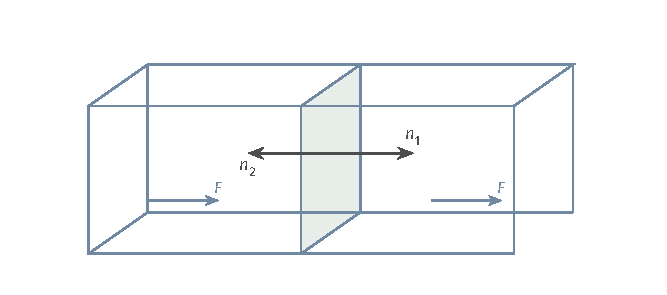
\includegraphics[width=112mm]{figures/01-mathematical-preliminaries-upper/00-shared/tikz/chapter3-concept-processes/gauss-shared-face.pdf}
 \caption{两个相邻单位立方体共用绿色面，图用斜投影表示三维几何。取常场$F=(1,0,0)^\top$，共同面上两侧外法向为$n_1=(1,0,0)^\top$与$n_2=-n_1$，对应通量为$1,-1$，相加抵消。整体外向净通量也为零，与散度为零一致；一般区域的散度定理仍需要前述条件与证明。}
 \label{fig:analysis-process-gauss-shared-face}
\end{figure}

先用一个答案已知的计算核对散度定理。
\begin{example}[用散度定理核对球面面积]
设$B_R$是以原点为中心、半径$R>0$的球，边界球面取外法向。令$\bm F(\bm x)=\bm x/R$，它在整个$\mathbb R^3$上连续可微。
球面上$\bm n=\bm x/R=\bm F$，所以$\bm F^\top\bm n=1$，外向通量等于球面面积。
另一方面，$\operatorname{div}\bm F=3/R$，散度定理给出
\[
 \int_{\partial B_R}\bm F^\top\bm n\,\mathrm dS
 =\frac3R\operatorname{vol}(B_R)
 =\frac3R\cdot\frac{4\pi R^3}3=4\pi R^2.
\]
\end{example}
这里的球体积已在第~\ref{sec:multivariable-change-variables}节用球坐标算出；所得结果与第~\ref{sec:analysis-surface-integration}节直接参数化球面求得的面积一致。

定理要求$\bm F$在$\overline\Omega$的一个开邻域内连续可微。点源场在原点无定义，下面用它检查这一条件的作用。
\begin{example}[点源的通量]
\label{ex:analysis-point-source-flux}
在$\mathbb R^3\setminus\{\bm0\}$上取$\bm F(\bm x)=\bm x/\lVert\bm x\rVert_2^3$，记$r=\lVert\bm x\rVert_2$。由$\partial_jr=x_j/r$，
\[
 \partial_j\Bigl(\frac{x_j}{r^3}\Bigr)=\frac1{r^3}-\frac{3x_j^2}{r^5},
 \qquad
 \operatorname{div}\bm F=\frac3{r^3}-\frac{3r^2}{r^5}=0.
\]
但在半径为$R$的球面上，外法向为$\bm x/R$，$\bm F^\top\bm n=1/R^2$，外向通量为$4\pi R^2/R^2=4\pi$。
这并不与散度定理矛盾：球体含有原点，而$\bm F$在原点无定义，定理的条件不满足。

对不含原点的球壳$R_1<r<R_2$，定理适用，左侧为零。外球面的外向通量为$4\pi$；内球面的外法向指向原点，通量为$-4\pi$；两者相加确为零。
\end{example}
所以以原点为中心的球面上的通量都是$4\pi$，与半径无关：场在原点以外处处无源，全部通量都来自原点处的点源。
静电学中，位于原点的点电荷$q$产生的电场是$\frac{q}{4\pi\varepsilon_0}\bm F$，其中$\varepsilon_0$为真空介电常数；它穿过以原点为中心的球面的通量为$q/\varepsilon_0$，这就是Gauss定律在点电荷上的形式。

\paragraph{散度是通量密度}

已证明的长方体情形，足以把散度一节的近似推导变成精确结论。
设$\bm F$在开集$U$上连续可微，$\bm a\in U$，$Q_h$是以$\bm a$为中心、边长为$h$的立方体；$h$足够小时$\overline{Q_h}\subseteq U$。由长方体上的Gauss公式，
\[
 \frac1{h^3}\int_{\partial Q_h}\bm F^\top\bm n\,\mathrm dS
 =\frac1{h^3}\int_{Q_h}\operatorname{div}\bm F\,\mathrm d\bm x.
\]
右侧是散度在$Q_h$上的平均值，它与$\operatorname{div}\bm F(\bm a)$的差不超过$\sup_{Q_h}|\operatorname{div}\bm F-\operatorname{div}\bm F(\bm a)|$。散度连续，所以$h\to0$时这个上界趋于零，平均值趋于$\operatorname{div}\bm F(\bm a)$。

这说明散度确实是“单位体积的净流出”的极限。把立方体换成以$\bm a$为中心的小球，用一般的Gauss公式可以得到同样的极限。小球的取法不依赖坐标轴，所以散度描述的是场本身的性质，不依赖坐标系的方向。

\subsubsection{多元分部积分}

一元分部积分（式~\eqref{eq:analysis-integration-by-parts}）把一个因子的导数转给另一个因子，并留下端点项。设$u$在$[a,b]$上连续可微、$v$二阶连续可微，把式中的$v$换成$v'$，得到
\[
 \int_a^bu\,v''\,\mathrm dx
 =u(b)v'(b)\cdot(+1)+u(a)v'(a)\cdot(-1)-\int_a^bu'v'\,\mathrm dx.
\]
这里把端点项$[uv']_a^b$拆开写：区间在右端点的外法向是$+1$，在左端点是$-1$。

推广到多元情形时，各项依次对应：二阶导数$v''$换成$\Delta v$，一阶导数的乘积$u'v'$换成梯度的内积$\nabla u^\top\nabla v$，两个端点换成边界曲面，“$v'$乘外法向$\pm1$”换成$\nabla v^\top\bm n$，即$v$沿外法向的方向导数。
对乘积向量场$u\nabla v$使用散度定理，就得到这一推广。
\begin{theorem}[多元分部积分]
\label{thm:multivariable-integration-by-parts}
设$\Omega\subseteq\mathbb R^3$满足上述Gauss公式的区域条件。
若标量函数$u$在$\overline\Omega$的开邻域内连续可微，$v$在同一邻域内二阶连续可微，则
\[
 \int_\Omega u\Delta v\,\mathrm d\bm x
 =\int_{\partial\Omega}u\nabla v^\top\bm n\,\mathrm dS
  -\int_\Omega\nabla u^\top\nabla v\,\mathrm d\bm x.
\]
\end{theorem}
\begin{proof}
向量场$\bm F=u\nabla v$的第$j$个分量是$u\,\partial_jv$，它连续可微。由一元乘积法则，
$\partial_j(u\,\partial_jv)=\partial_ju\,\partial_jv+u\,\partial_j^2v$，对$j$求和得到
\[
 \operatorname{div}(u\nabla v)
 =\nabla u^\top\nabla v+u\Delta v.
\]
将它代入Gauss公式，再把$\nabla u^\top\nabla v$的区域积分移到等式另一侧，即得结论。
\end{proof}
对满足Green公式条件的平面区域，同样的证明改用平面通量公式（定理~\ref{thm:multivariable-planar-flux}）即可，边界面积元素相应换成弧长元素。
这一公式把$v$的二阶导数转移为$u$与$v$的一阶导数，同时保留法向边界项；该项是否为零，必须由具体边界条件决定。

取$u=1$，公式化为$\int_\Omega\Delta v\,\mathrm d\bm x=\int_{\partial\Omega}\nabla v^\top\bm n\,\mathrm dS$，也就是对梯度场$\nabla v$使用散度定理。下面在球上核对这一特例。
\begin{example}[球上平方范数的Laplace积分]
取以原点为中心、半径为$R$的球$B_R$和$v(\bm x)=\lVert\bm x\rVert_2^2$。
左侧：$\Delta v=6$，所以$\int_{B_R}\Delta v\,\mathrm d\bm x=6\operatorname{vol}(B_R)=6\cdot\frac{4\pi R^3}3=8\pi R^3$。
右侧：球面上$\nabla v=2\bm x$，外法向$\bm n=\bm x/R$，故$\nabla v^\top\bm n=2\lVert\bm x\rVert_2^2/R=2R$，积分为$2R\cdot4\pi R^2=8\pi R^3$。两侧相等。
\end{example}

边界项为零时，公式可以给出结构性的结论。下面用它说明Laplace方程的解由边界值唯一确定。
\begin{example}[Laplace方程的解由边界值决定]
设$\Omega$满足Gauss公式的区域条件，$w$在$\overline\Omega$的开邻域内二阶连续可微，在$\Omega$内$\Delta w=0$，在$\partial\Omega$上$w=0$。
在定理~\ref{thm:multivariable-integration-by-parts}中取$u=v=w$。左侧被积函数$w\Delta w$为零；边界项的被积函数含因子$w$，也为零。于是
\[
 \int_\Omega\lVert\nabla w\rVert_2^2\,\mathrm d\bm x=0.
\]
被积函数连续且非负；若它在某点为正，则在该点的一个邻域内为正，积分也为正。所以在开集$\Omega$上$\nabla w$恒为零。
$\Omega$是连通的开区域，所以$w$在$\Omega$上为常数；再由$w$在$\overline\Omega$上连续且在边界上为零，得$w\equiv0$。

现在设$v_1,v_2$都在$\overline\Omega$的开邻域内二阶连续可微，在$\Omega$内满足$\Delta v_1=\Delta v_2=0$，在$\partial\Omega$上取值相同。差$w=v_1-v_2$满足上面的全部条件，所以$v_1=v_2$。
\end{example}
按热传导的解释，稳定的温度分布由边界温度唯一决定。

\subsection{曲面积分与边界路径积分}

Gauss公式要求闭曲面围成空间区域。另一类问题只给一张有边界的定向曲面，要求比较曲面上的旋转累计与边界环流。
这时使用旋度在曲面法向上的分量，不需要先把曲面补成闭曲面。

\subsubsection{Stokes公式}

在$z=0$平面上取向上法向时，旋度的法向分量$(\nabla\times\bm F)^\top\bm e_3$就是Green公式中的$Q_x-P_y$。
对空间中的弯曲曲面，可以把它切成许多很小的曲面片，每片近似是一小块平面。在法向为$\bm n$的小平面片上，边界环流约等于$(\nabla\times\bm F)^\top\bm n$乘面积。
各片采用相容定向时，相邻两片的公共边被沿相反方向走过，环流相消，只剩整张曲面的边界。
用桨轮的图像说：在曲面上各处放置转轴沿法向的小桨轮，它们感受到的旋转强度按面积累加，总和等于沿曲面边缘走一圈的环流。
Stokes公式把这一关系写成精确等式，同时要求法向与边界方向相容。
\begin{theorem}[Stokes定理]
\label{thm:multivariable-stokes}
设$S\subseteq\mathbb R^3$为紧致、可定向的分片$C^2$曲面，边界由有限条分段$C^1$简单闭曲线组成。
各光滑曲面片选取连续且片间定向相容的单位法向$\bm n$，边界采用其诱导方向。
若向量场$\bm F$在$S$的开邻域内连续可微，则\term{Stokes公式}（Stokes' theorem）给出
\begin{equation}
 \oint_{\partial S}\bm F^\top\,\mathrm d\bm r
 =\int_S(\nabla\times\bm F)^\top\bm n\,\mathrm dS.
 \label{eq:multivariable-stokes}
\end{equation}
\end{theorem}
这里的“可定向”要求各曲面片能相容地选择法向，使公共边上的诱导方向相反；有折角的接缝处不要求存在唯一法向。
两侧都为标量：左侧是原向量场的边界环流，右侧是其旋度穿过曲面的通量。

在一张参数曲面片上，可以把公式归结为参数平面上的Green公式。
设参数域$D$满足Green公式的区域条件，$\bm r(u,v)$在$D$的邻域内二阶连续可微、在内部正则且一一对应，并采用$\bm r_u\times\bm r_v$确定的定向。
还要求$\partial D$的正向经$\bm r$对应曲面片边界的诱导方向，从而可以把边界路径积分放到$\partial D$上计算。
这里的$u,v$是参数，与多元分部积分中的函数$u,v$无关。记
\[
 \begin{aligned}
 A(u,v)&=\bm F(\bm r(u,v))^\top\bm r_u(u,v),\\
 B(u,v)&=\bm F(\bm r(u,v))^\top\bm r_v(u,v).
 \end{aligned}
\]

先处理左侧。若$(u(t),v(t))$沿$\partial D$行进，曲面边界上对应的点是$\bm r(u(t),v(t))$，由链式法则，其速度为$\bm r_uu'(t)+\bm r_vv'(t)$。
与$\bm F$取内积，得$\bm F^\top\mathrm d\bm r=A\,\mathrm du+B\,\mathrm dv$，所以左侧等于参数平面上的路径积分$\oint_{\partial D}A\,\mathrm du+B\,\mathrm dv$。

再计算参数平面上Green公式右侧的被积函数$\partial_uB-\partial_vA$。记$\bm J_{\bm F}$为$\bm F$的Jacobian矩阵，其元素为$(\bm J_{\bm F})_{i,j}=\partial_jF_i$。由链式法则和乘积法则，
\[
 \begin{aligned}
 \partial_uB&=(\bm J_{\bm F}\bm r_u)^\top\bm r_v+\bm F^\top\bm r_{vu},\\
 \partial_vA&=(\bm J_{\bm F}\bm r_v)^\top\bm r_u+\bm F^\top\bm r_{uv},
 \end{aligned}
\]
其中$\bm J_{\bm F}$与$\bm F$在$\bm r(u,v)$处取值。$\bm r$二阶连续可微，混合偏导相等，$\bm r_{uv}=\bm r_{vu}$，所以两式相减时含二阶导数的项抵消。
又$(\bm J_{\bm F}\bm r_u)^\top\bm r_v=\bm r_v^\top\bm J_{\bm F}\bm r_u$、$(\bm J_{\bm F}\bm r_v)^\top\bm r_u=\bm r_v^\top\bm J_{\bm F}^\top\bm r_u$，于是
\[
 \partial_uB-\partial_vA=\bm r_v^\top(\bm J_{\bm F}-\bm J_{\bm F}^\top)\bm r_u.
\]

接下来把右端写成旋度。反对称矩阵$\bm W=\bm J_{\bm F}-\bm J_{\bm F}^\top$的元素为$\bm W_{i,j}=\partial_jF_i-\partial_iF_j$；逐个分量对照旋度的定义可以验证，对任意$\bm a\in\mathbb R^3$都有$\bm W\bm a=(\nabla\times\bm F)\times\bm a$。
再用混合积的轮换关系$\bm b^\top(\bm c\times\bm a)=\bm c^\top(\bm a\times\bm b)$（两边都等于以$\bm a,\bm b,\bm c$为列的行列式），取$\bm a=\bm r_u$、$\bm b=\bm r_v$、$\bm c=\nabla\times\bm F$，得到
\[
 \partial_uB-\partial_vA
 =\bigl(\operatorname{curl}\bm F\bigr)(\bm r(u,v))^\top
   (\bm r_u\times\bm r_v).
\]
右端乘$\mathrm du\,\mathrm dv$，正是曲面通量积分（式~\eqref{eq:analysis-surface-flux}）中的被积项。

$A,B$由连续可微的$\bm F$与二阶连续可微的$\bm r$及其一阶导数复合、相乘而成，在$D$的邻域内连续可微，所以参数平面上的Green公式适用；它给出该曲面片上的Stokes公式。
对有限张相容定向的曲面片，公共边的路径积分相消，只剩整张曲面的边界。
一般分片曲面的完整论证还需核对曲面覆盖及接缝条件；以上推导只说明参数片上的机制，一般定理可参考向量微积分教材\scite{math-strang1991calculus}。

\paragraph{旋度分量是环流密度}

Stokes公式也给出旋度含义的精确形式。设$\bm F$在$\bm a$附近连续可微，$\bm n$是单位向量，$D_\rho$是以$\bm a$为圆心、半径为$\rho$、垂直于$\bm n$并取法向$\bm n$的平面圆盘。由Stokes公式，
\[
 \frac1{\pi\rho^2}\oint_{\partial D_\rho}\bm F^\top\,\mathrm d\bm r
 =\frac1{\pi\rho^2}\int_{D_\rho}(\nabla\times\bm F)^\top\bm n\,\mathrm dS,
\]
右侧是$(\nabla\times\bm F)^\top\bm n$在圆盘上的平均值。旋度连续，所以$\rho\to0$时它趋于$(\nabla\times\bm F)(\bm a)^\top\bm n$。
因此，旋度沿$\bm n$的分量就是垂直于$\bm n$的微小圆周上的环流除以所围面积的极限。这正是桨轮图像所描述的量；圆盘的取法不依赖坐标轴，所以这一含义也不依赖坐标轴的选取。

\subsubsection{跨接曲面的选择}

Stokes公式的左侧只由有向边界和边界上的向量场决定。因此，若两张满足定理条件的定向曲面具有同一有向边界，
且$\bm F$在两张曲面附近都连续可微，则两张曲面上的旋度通量相等。
计算时可以选较简单的跨接曲面，但必须核对向量场定义域，不能让替换曲面穿过场的奇点。

这一结论也可以从Gauss公式得到印证。若$\bm F$二阶连续可微，则
\[
 \operatorname{div}(\nabla\times\bm F)
 =\partial_x(\partial_yF_3-\partial_zF_2)
 +\partial_y(\partial_zF_1-\partial_xF_3)
 +\partial_z(\partial_xF_2-\partial_yF_1)=0,
\]
最后的等号成立，是因为混合偏导相等，六项两两抵消。设两张跨接曲面恰好围成一个满足Gauss公式条件的区域，且$\bm F$在该区域闭包的开邻域内二阶连续可微。
区域的外法向在一张曲面上与所选法向相同，在另一张上相反；旋度场的散度为零，所以散度定理说明两张曲面上的旋度通量之差为零。

下面用同一个场在单位圆上比较两张跨接曲面。
\begin{example}[单位圆上的圆盘与半球面]
取$\bm F=(-y/2,x/2,0)^\top$，它在整个$\mathbb R^3$上连续可微，示例~\ref{ex:analysis-rigid-rotation-curl}已算出$\nabla\times\bm F=(0,0,1)^\top$。单位圆$\{x^2+y^2=1,\ z=0\}$采用从上方看逆时针的方向。

先取向上单位圆盘$S_1$。由示例~\ref{ex:analysis-hemisphere-induced-orientation}，它的诱导方向正是这一方向；旋度的法向分量为$1$，所以
\[
 \oint_{\partial S_1}\bm F^\top\,\mathrm d\bm r
 =\iint_{S_1}1\,\mathrm dS=\pi.
\]
直接计算左侧也得到同一结果：取$\gamma(t)=(\cos t,\sin t,0)^\top$，$0\leq t\leq2\pi$，则$\bm F(\gamma(t))^\top\gamma'(t)=\tfrac12(\sin^2t+\cos^2t)=\tfrac12$，积分为$\pi$。

再取外向上半单位球面$S_2$，同一例子说明它的诱导方向与$S_1$相同。用第~\ref{sec:analysis-surface-integration}节的球面参数$(\varphi,\theta)$，$0\leq\varphi\leq\pi/2$，外法向为$\bm n=\bm x$，旋度的法向分量为$z=\cos\varphi$，面积元为$\sin\varphi\,\mathrm d\varphi\,\mathrm d\theta$，所以
\[
 \int_{S_2}(\nabla\times\bm F)^\top\bm n\,\mathrm dS
 =\int_0^{2\pi}\int_0^{\pi/2}\cos\varphi\sin\varphi\,\mathrm d\varphi\,\mathrm d\theta
 =2\pi\cdot\frac12=\pi,
\]
与圆盘上的结果相同。
\end{example}
若改用向下定向的圆盘，边界方向也必须反转，两个积分同时变号。


图~\ref{fig:analysis-process-stokes-spanning-surfaces}比较同一有向圆周的两张跨接曲面。替换曲面时，边界方向与场的定义域都要同时保留。
\begin{figure*}[!htbp]
 \centering
 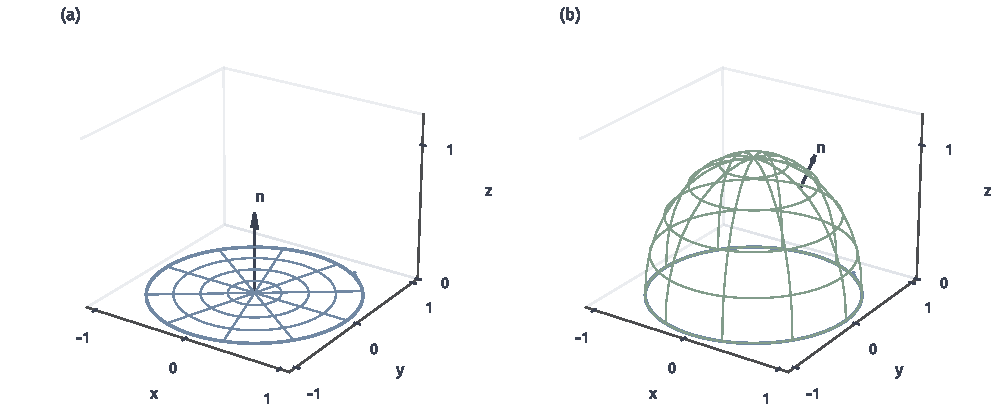
\includegraphics[width=169.0mm]{figures/01-mathematical-preliminaries-upper/00-shared/matplotlib/chapter3-concept-processes/stokes-spanning-surfaces.pdf}
 \caption{(a) 向上单位圆盘；(b) 外向上半单位球面。蓝色边界均从上方看逆时针，黑箭头标记各自法向。对$F=(-y/2,x/2,0)^\top$，旋度恒为$(0,0,1)^\top$，两面上的旋度通量都为$\pi$。右面面积为$2\pi$而非$\pi$；相等的是法向分量的累计，不能把通量当成面积。}
 \label{fig:analysis-process-stokes-spanning-surfaces}
\end{figure*}

\subsection{积分公式的比较}

本节各公式回答的都是同一类问题：导数在内部的积分与边界积分之间的关系。推导方式也相同：在小块上建立局部关系，再利用相容方向让内部边界相消。
它们的内部对象、边界对象和方向条件则各不相同。下表把一元基本定理与路径积分基本定理也列在一起，二者以区间或路径的两个端点为边界。
\begin{center}
\begin{tabular}{lll}
\toprule
公式 & 内部积分 & 边界积分\\
\midrule
一元基本定理 & 区间上的$f'$ & 端点值之差$f(b)-f(a)$\\
路径积分基本定理 & 路径上$\nabla\phi$的切向积分 & 端点值之差\\
Green环流形式 & 平面区域的$Q_x-P_y$ & 正向路径的切向积分\\
Gauss & 空间区域的散度 & 闭曲面的外向通量\\
Stokes & 定向曲面的旋度通量 & 诱导方向的路径环流\\
\bottomrule
\end{tabular}
\end{center}
对向上定向的平面曲面，Stokes公式还原为Green公式的环流形式；Green公式的通量形式则是二维的散度公式。
普通标量函数的区域积分不自动具有边界表达：要使用这些公式，须先找到满足条件的向量场，使其散度或旋度的相应分量等于被积函数。示例~\ref{ex:analysis-green-area-formula}的面积公式就是先选出满足$Q_x-P_y\equiv1$的场。

Stokes公式还解释了第~\ref{sec:multivariable-potential-path-independence}节中势函数的存在为何与定义域有关。设$\bm F$在开集$U\subseteq\mathbb R^3$上连续可微且$\nabla\times\bm F=\bm0$。若一条闭路径是$U$内某张满足定理条件的定向曲面的有向边界，则该闭路径上的环流等于旋度的通量，也就是零。
在星形域中，闭路径上各点与中心点之间的线段扫出一张锥面，它整个落在定义域内，不会碰到场的奇点；这与那里在星形域上构造势函数的结论一致。
穿孔平面上绕原点的单位圆则不同：在平面内，以它为边界的区域只能是单位圆盘，必然包含原点，而场在原点无定义；所以局部条件$Q_x-P_y=0$并不排除$2\pi$的环流（示例~\ref{ex:analysis-annulus-vortex-green}）。

各公式均使用勒贝格积分。连续可微性、分片规则边界与定向是这里的经典公式所需的条件，并不是另换一种积分定义。
尤其要核对向量场是否在整个积分对象附近都有定义：穿孔平面上的涡旋场在原点无定义，不能把包含原点的圆盘直接代入Green公式；点源场也不能直接用于包含原点的球体（示例~\ref{ex:analysis-point-source-flux}）。
区域积分不能区分只在零测集上不同的函数，而本节区域的边界由有限条曲线或有限个曲面片组成，在相应的面积或体积测度下正是零测集；所以仅知道两个函数在区域上几乎处处相等，不足以确定它们的边界积分。
如果要降低导数或边界的规则性，还须另外建立弱导数、边界迹及相应的积分公式；不能沿用当前公式而省去这些条件。

\FloatBarrier


\FloatBarrier
\section{本章小结}
\label{sec:multivariable-summary}

多元函数的极限要求所有趋近方式给出同一结果，只检查坐标轴或直线还不够。可微要求所有小扰动共用同一个线性映射：梯度给出最快上升的方向，Jacobian矩阵描述小方格怎样被拉伸成小平行四边形，Hessian矩阵描述函数沿各方向的弯曲，并据此区分极小点、极大点和鞍点。
偏导数存在、方向导数存在、可微与连续可微是逐步加强的条件，各级之间都有反例。凸区域上，梯度长度的上界就是Lipschitz常数。

区域积分把密度累计成总量；Tonelli与Fubini定理说明何时可以逐个坐标切片计算，Jacobian行列式的绝对值给出坐标变换下的体积缩放。
第一类路径积分与曲面积分按弧长和面积累计，不依赖方向；第二类路径积分计算做功，第二类曲面积分计算通量，二者都随方向反转而变号。
保守场的功只取决于端点，交叉偏导相等在星形区域上保证势函数存在，在有孔的区域上则不够。

散度是单位体积的净流出，旋度是单位面积的环流。Green、Gauss和Stokes公式把内部的散度或旋度累计等同于边界上的通量或环流，是一元微积分基本定理在多维中的推广；使用时要逐一核对光滑性、可积性和边界定向条件。
